% =====================================================================
% PART I REBUILD — SIX-PAGE OPENING
% The machine is not presented in advance. Each component appears only
% after a physical failure makes it necessary.
% Build from the repository root: python3 thesis/code/build.py thesis
% =====================================================================
\documentclass[11pt]{article}
\usepackage[letterpaper,margin=0.82in]{geometry}
\usepackage{amsmath,amssymb,mathtools}
\usepackage{graphicx}
\usepackage{xcolor}
\usepackage{tikz}
\usepackage[colorlinks=true,linkcolor=blue,urlcolor=blue]{hyperref}
\setlength{\parindent}{0pt}
\setlength{\parskip}{5pt}
\setlength{\fboxsep}{8pt}
\newcommand{\designconsequence}[1]{%
  \begin{center}\fcolorbox{black!50}{black!3}{\parbox{0.90\textwidth}{%
  \textbf{Design consequence.} #1}}\end{center}}
\newcommand{\model}[1]{\textit{Model and limits.} #1}
\newcommand{\auditnote}[1]{%
  \begin{center}\fcolorbox{red!60!black}{red!4}{\parbox{0.90\textwidth}{%
  \textbf{Audit note.} #1}}\end{center}}
\newcommand{\supportingquantity}[2]{%
  \noindent\textit{Supporting quantity --- #1.} #2\par}
\newcommand{\friedbergvariable}[2]{%
  \begin{center}\fcolorbox{blue!60!black}{blue!5}{\parbox{0.90\textwidth}{%
  \textbf{Primary Friedberg parameter --- #1.} #2}}\end{center}}
\newcommand{\imagebrief}[2]{%
  \begin{center}\fcolorbox{orange!80!black}{yellow!12}{\parbox{0.90\textwidth}{%
  \textbf{PLACE IMAGE HERE --- #1.} {\footnotesize #2}}}\end{center}}

\title{Part I --- Let the Machine Reveal Itself\\
\large A first-principles route to the tokamak}
\author{Jony (TUNEM)}
\date{Rebuilt opening, August 2026}

\newcommand{\schematicnote}{\emph{Idealized schematic; not a fabrication drawing.}}
\begin{document}

% ============================== PAGE 1 ==============================
\maketitle
\vspace{-1.5em}

\textbf{Promise to the reader.} We will not begin by displaying a tokamak and asking
you to accept its parts. We will begin with a desired physical event---controlled
deuterium--tritium fusion---and let each failure of the simplest attempted design force
the next component into existence. Every load-bearing equation will either be derived
where it appears or tied to an accessible source. An approximation will be named before
it is used.

\section*{1. The first requirement: make nuclei approach}

The reaction chosen by nearly every near-term fusion-power design is
\begin{equation}
 {}^{2}\mathrm H+{}^{3}\mathrm H\longrightarrow{}^{4}\mathrm{He}\;(3.5\,\mathrm{MeV})
 +n\;(14.1\,\mathrm{MeV}), \qquad Q=17.6\,\mathrm{MeV}.\label{eq:dt}
\end{equation}
The released energy is the decrease in rest mass multiplied by $c^2$. The products
share it in inverse proportion to their masses because momentum is conserved: the
lighter neutron carries about four fifths and the alpha particle about one fifth. These
numbers will later decide which energy remains in the plasma and which must be caught by
a blanket. For now, the obstacle comes before the reward.

A deuteron and triton both carry charge $+e$. At separation $r$ their electrostatic
potential energy is
\begin{equation}
 U(r)=\frac{e^2}{4\pi\epsilon_0 r}.\label{eq:coulomb}
\end{equation}
At $r=2\,\mathrm{fm}$, a nuclear length scale, Eq.~\eqref{eq:coulomb} is about
$0.72\,\mathrm{MeV}$.
A classical particle would need a comparable collision energy to reach that distance.
Fusion plasmas operate at much lower thermal energies, typically $T\sim10$--$20\,\mathrm{keV}$,
because quantum tunnelling gives some collisions a finite probability of crossing the
remaining barrier. Temperature is being measured in energy units: $T$ means $k_BT$.
Thus
\[
10\,\mathrm{keV}=10^4\,\mathrm{eV}
\quad\Longleftrightarrow\quad
T_K=\frac{10^4\,\mathrm{eV}}{k_B}=1.16\times10^8\,\mathrm K.
\]
This does not mean every ion has the same energy. It means the distribution has a hot
tail; fusion occurs disproportionately in that tail. A later section will derive the
Gamow peak and the reaction rate. Here we need only the first unavoidable conclusion.

\designconsequence{Useful D--T fusion requires matter at roughly one hundred million
kelvin. Sustained contact with a material surface would cool and contaminate the plasma,
while reactor heat flux would erode and damage the surface. The fuel must therefore be
kept in vacuum and away from material walls.}

\vfill
{\footnotesize Reaction data and the reactor-design context are reproduced in
J.~P. Freidberg, F.~J. Mangiarotti, and J.~Minervini, ``Designing a Tokamak Fusion
Reactor---How Does Plasma Physics Fit In?'' (2015), open manuscript:
\url{https://library.psfc.mit.edu/catalog/reports/2010/15ja/15ja021/15ja021_full.pdf}.}
\newpage

% ============================== PAGE 2 ==============================
\section*{2. The handle nature gives us: charged particles}

At $10\,\mathrm{keV}$, the thermal energy is hundreds of times larger than the
$13.6\,\mathrm{eV}$ binding energy of ground-state hydrogen. Deuterium and tritium do
not remain neutral atoms: electrons are stripped from their nuclei. The result is a
\emph{plasma}, containing positive ions and negative electrons.

The plasma is not, as a whole, a charged ball. On length scales large compared with a
small electrostatic screening length, its positive and negative charge densities nearly
cancel: it is \emph{quasineutral}. The useful fact is subtler. Its constituent particles
carry charge, so electromagnetic fields can redirect them without a material surface.

For a particle of mass $m$, charge $q$, and velocity $\mathbf v$, the Lorentz equation is
\begin{equation}
 m\frac{d\mathbf v}{dt}=q\big(\mathbf E+\mathbf v\times\mathbf B\big).\label{eq:lorentz}
\end{equation}
Set $\mathbf E=0$ temporarily and take a uniform field
$\mathbf B=B\hat{\mathbf z}$. Dotting Eq.~\eqref{eq:lorentz} with $\mathbf v$ gives
\[
\frac{d}{dt}\left(\frac12m|\mathbf v|^2\right)
=q\,\mathbf v\cdot(\mathbf v\times\mathbf B)=0.
\]
The magnetic force changes direction but not kinetic energy. It is therefore a steering
force, not a refrigerator and not a source of free plant power.

Write $w=v_x+i v_y$. The perpendicular components of Eq.~\eqref{eq:lorentz} become
\[
\dot v_x=\frac{qB}{m}v_y,\qquad
\dot v_y=-\frac{qB}{m}v_x,
\qquad\Longrightarrow\qquad
\dot w=-i\frac{qB}{m}w.
\]
Hence $w(t)=w(0)e^{-iqBt/m}$: the perpendicular velocity rotates. Integrating once,
the particle follows a circle of radius
\begin{equation}
 \omega_c=\frac{|q|B}{m},\qquad
 r_L=\frac{v_\perp}{\omega_c}=\frac{m v_\perp}{|q|B}.\label{eq:gyro}
\end{equation}
Meanwhile the parallel component obeys $\dot v_z=0$. The full orbit is a helix: a
small circle across the field combined with free streaming along it.

For a $10\,\mathrm{keV}$ deuteron in $3\,\mathrm T$,
$v_\perp=\sqrt{2T/m_D}=9.8\times10^5\,\mathrm{m/s}$ and
$r_L=6.8\,\mathrm{mm}$. A magnetic field can therefore keep transverse excursions
small compared with a metre-scale chamber. Equation~\eqref{eq:gyro}, however, exposes the failure:
it does nothing to stop motion along the field.

\designconsequence{The ``invisible wall'' cannot be a wall in the ordinary sense. It
must be a set of magnetic field lines that guide charged particles, and those lines
must eventually have no open ends.}

\newpage

% ============================== PAGE 3 ==============================
\section*{3. First attempted machine: a straight magnetic corridor}

Before closing the ends, we must make a field. Electric current is its source. In a
static situation Amp\`ere's law is
\begin{equation}
 \oint_C\mathbf B\cdot d\boldsymbol\ell=\mu_0 I_{\rm linked}.\label{eq:ampere}
\end{equation}
Wind wire into many circular turns around a long cylinder. If there are $n$ turns per
unit length, take a rectangular Amp\`ere loop with one long side of length $L$ inside
the winding and the other far outside. For an ideal long solenoid, the exterior field
is negligible and the two short sides are perpendicular to $\mathbf B$.
Equation~\eqref{eq:ampere}
then gives
\begin{equation}
 BL=\mu_0(nL)I,\qquad\text{so}\qquad B\simeq\mu_0 nI.
\label{eq:solenoid}\end{equation}
This is our first actual component: a current-carrying coil. Its job is not yet to heat
or shape the fuel. Its job is to create the field that makes the gyro-orbits of
Eq.~\eqref{eq:gyro}.

\begin{center}
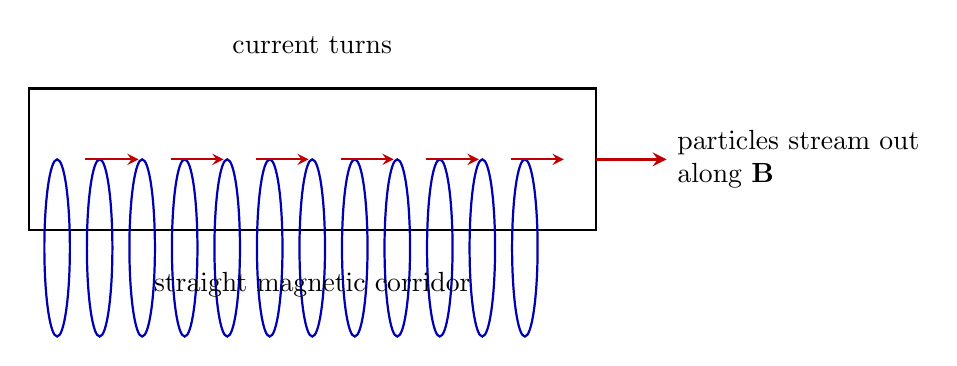
\begin{tikzpicture}[scale=0.90,>=stealth]
  \draw[thick] (-4,-1.0) rectangle (4,1.0);
  \foreach \x in {-3.6,-3.0,...,3.6}{
    \draw[blue!70!black,thick] (\x,-1.25) ellipse (0.18 and 1.25);
  }
  \foreach \x in {-3.2,-2.0,...,3.2}{
    \draw[red!75!black,->,thick] (\x,0) -- ++(0.75,0);
  }
  \draw[red!75!black,->,very thick] (4.0,0) -- (5.0,0)
    node[right,black,align=left]{particles stream out\\along $\mathbf B$};
  \node[above] at (0,1.35) {current turns};
  \node[below] at (0,-1.45) {straight magnetic corridor};
\end{tikzpicture}
\end{center}

The corridor controls cross-field motion, but Eq.~\eqref{eq:lorentz} already told us that
$v_\parallel$ remains free. At the deuteron speed above, a particle crosses a
$10\,\mathrm m$ device in roughly
\[
 t_{\rm end}\sim\frac{L}{v_\parallel}\sim
 \frac{10\,\mathrm m}{10^6\,\mathrm{m/s}}=10\,\mu\mathrm s.
\]
Making the straight corridor stronger reduces $r_L$ but does not change this end-loss
time. Magnetic mirrors can reflect some pitch angles, but particles within their loss
cone still escape. We have learned something more valuable than a failed design: the
problem is topological, not merely quantitative.

\designconsequence{Do not try to plug the ends of the magnetic corridor. Remove the
ends by joining them. The simplest closed version of a tube is a torus.}

\model{Equation~\eqref{eq:solenoid} assumes a solenoid long compared with its radius. End fields and
finite-coil corrections are deliberately omitted because the calculation is being used
to expose, not conceal, end loss.}

\newpage


\begin{figure}[htbp]\centering
  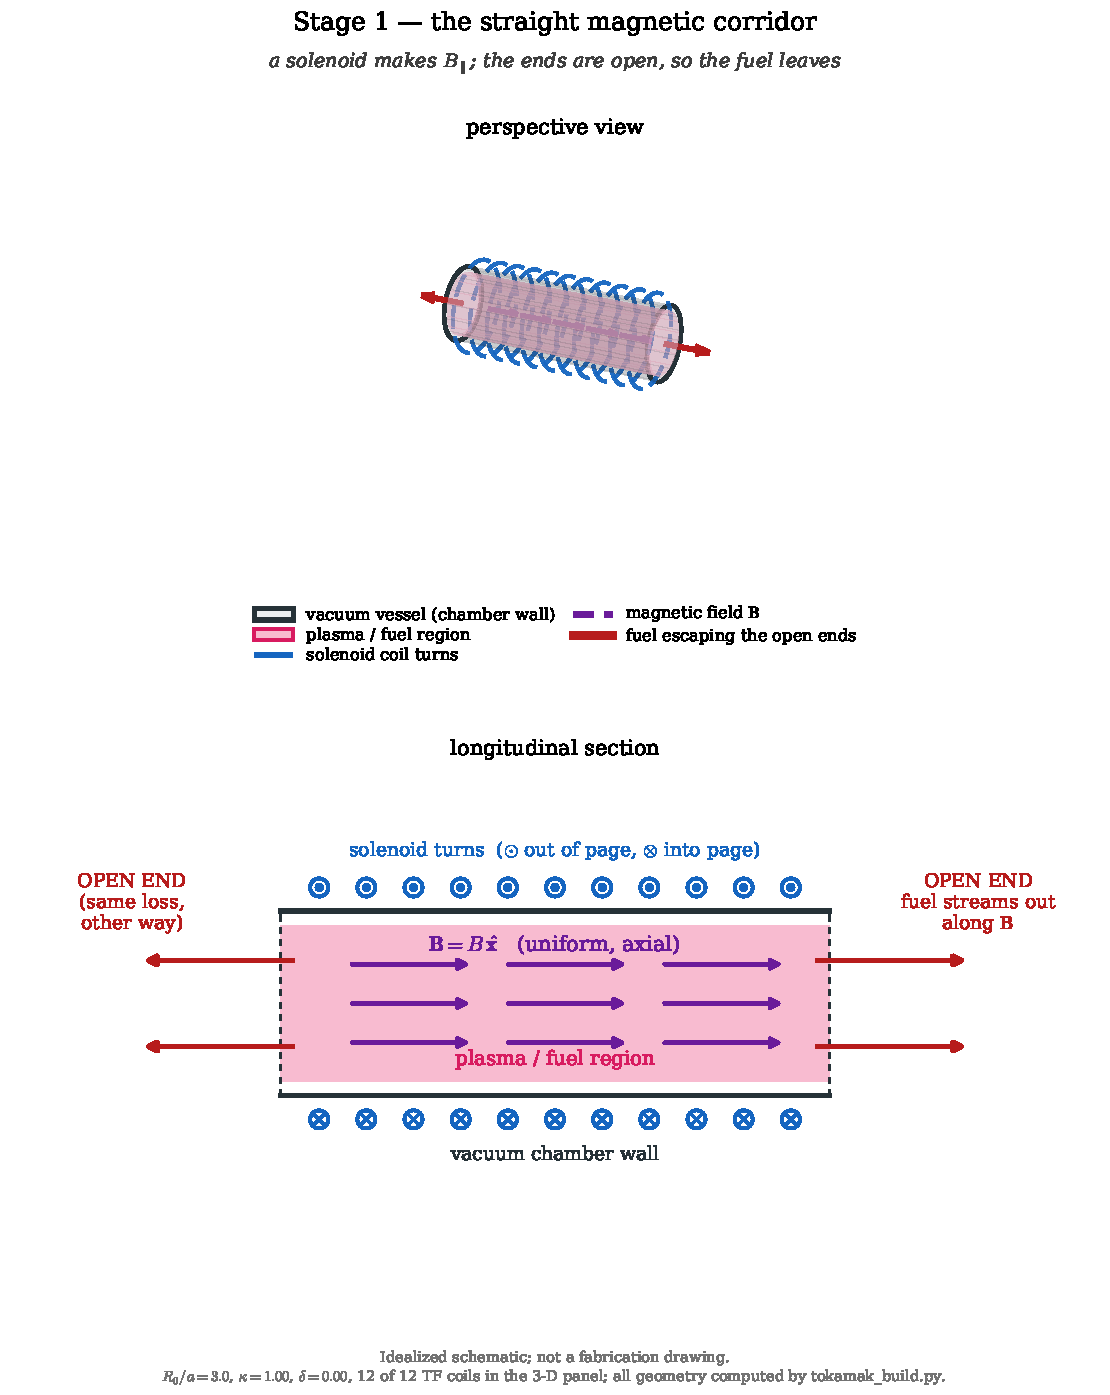
\includegraphics[width=1.0\textwidth]{figures/final/figM1_stage1_tall.pdf}
  \caption{The first machine state. A solenoid makes the field; the corridor has open ends, which is the failure the next section names.}
  \label{fig:figM1_stage1_tall}
\end{figure}

% ============================== PAGE 4 ==============================
\section*{4. Closing the corridor creates the torus}

Bend the straight magnetic corridor until its two ends meet. The field now runs the
long way around a torus; this direction is called \emph{toroidal}. A cross-section of
the tube has radius $a$, while the distance from the symmetry axis to the centre of that
cross-section is the major radius $R_0$:
\begin{equation}
 A\equiv\frac{R_0}{a}\qquad\text{(aspect ratio).}
\label{eq:aspect}
\end{equation}
These parameters have appeared because the design has acquired two geometrically
different lengths, not because a tokamak diagram handed them to us.

\friedbergvariable{$a$ (minor radius) and $R_0$ (major radius)}{Closing the
straight corridor makes these two dimensions unavoidable: $a$ measures the
cross-sectional reach available to the plasma, while $R_0$ measures the radius of
the closed path that removes end loss. Their ratio $A=R_0/a$ is useful, but is a
derived supporting quantity rather than an additional primary parameter.}

How do coils make a toroidal field? Arrange current-carrying loops around the torus so
that, in the ideal limit of continuously distributed coils, the system is axisymmetric.
Apply Amp\`ere's law to a circle of radius $R$ centred on the symmetry axis. The field is
tangent to the circle and constant along it, while the loop links total current $NI_c$:
\begin{equation}
 2\pi R B_\varphi(R)=\mu_0NI_c,
 \qquad
 \boxed{B_\varphi(R)=\frac{\mu_0NI_c}{2\pi R}}.
\label{eq:btor}
\end{equation}
Thus the toroidal field is intrinsically stronger on the inboard side and weaker on the
outboard side. Across a circular plasma,
\begin{equation}
 \frac{B_{\rm in}}{B_{\rm out}}
 =\frac{R_0+a}{R_0-a}=\frac{A+1}{A-1}.
\label{eq:fieldratio}
\end{equation}

\begin{center}
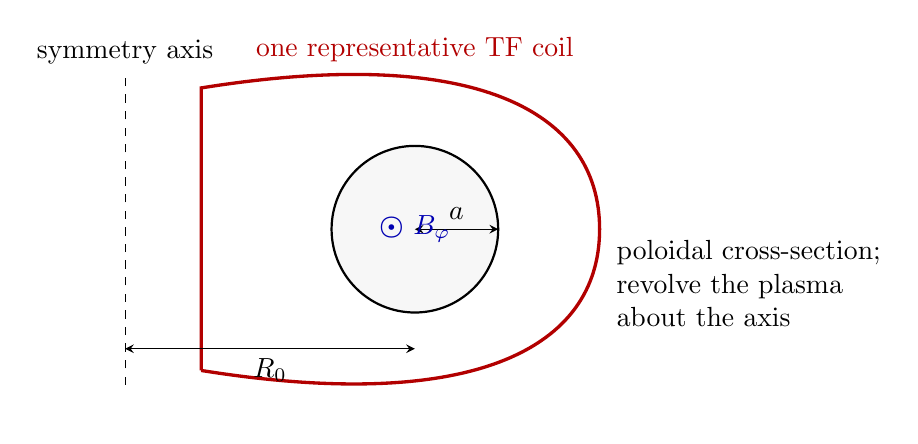
\begin{tikzpicture}[scale=0.92,>=stealth]
  \draw[dashed] (0,-2.15) -- (0,2.15) node[above]{symmetry axis};
  \draw[red!70!black,very thick]
    (1.05,-1.95) -- (1.05,1.95)
    .. controls (4.8,2.55) and (6.55,1.65) .. (6.55,0)
    .. controls (6.55,-1.65) and (4.8,-2.55) .. (1.05,-1.95);
  \node[red!70!black,above] at (4.0,2.18) {one representative TF coil};
  \draw[thick,fill=black!3] (4,0) circle (1.15);
  \draw[<->] (0,-1.65) -- node[below]{$R_0$} (4,-1.65);
  \draw[<->] (4,0) -- node[above]{$a$} (5.15,0);
  \node[blue!70!black] at (4,0) {$\boldsymbol\odot\ B_\varphi$};
  \node[right,align=left] at (6.65,-0.75) {poloidal cross-section;\\revolve the plasma\\about the axis};
\end{tikzpicture}
\end{center}

We have now removed the ends. We have not yet built a tokamak. The object presently on
the page is only a toroidal magnetic bottle, and Eq.~\eqref{eq:btor} has introduced a new asymmetry:
the field strength varies across the tube. The next question is whether this closed
field actually confines a particle.

\model{Equation~\eqref{eq:btor} is exact for the axisymmetric continuous-coil idealization. A finite
number of real toroidal-field coils produces ripple and a small external stray field;
those are later engineering corrections, not erased facts.}

\newpage


\begin{figure}[htbp]\centering
  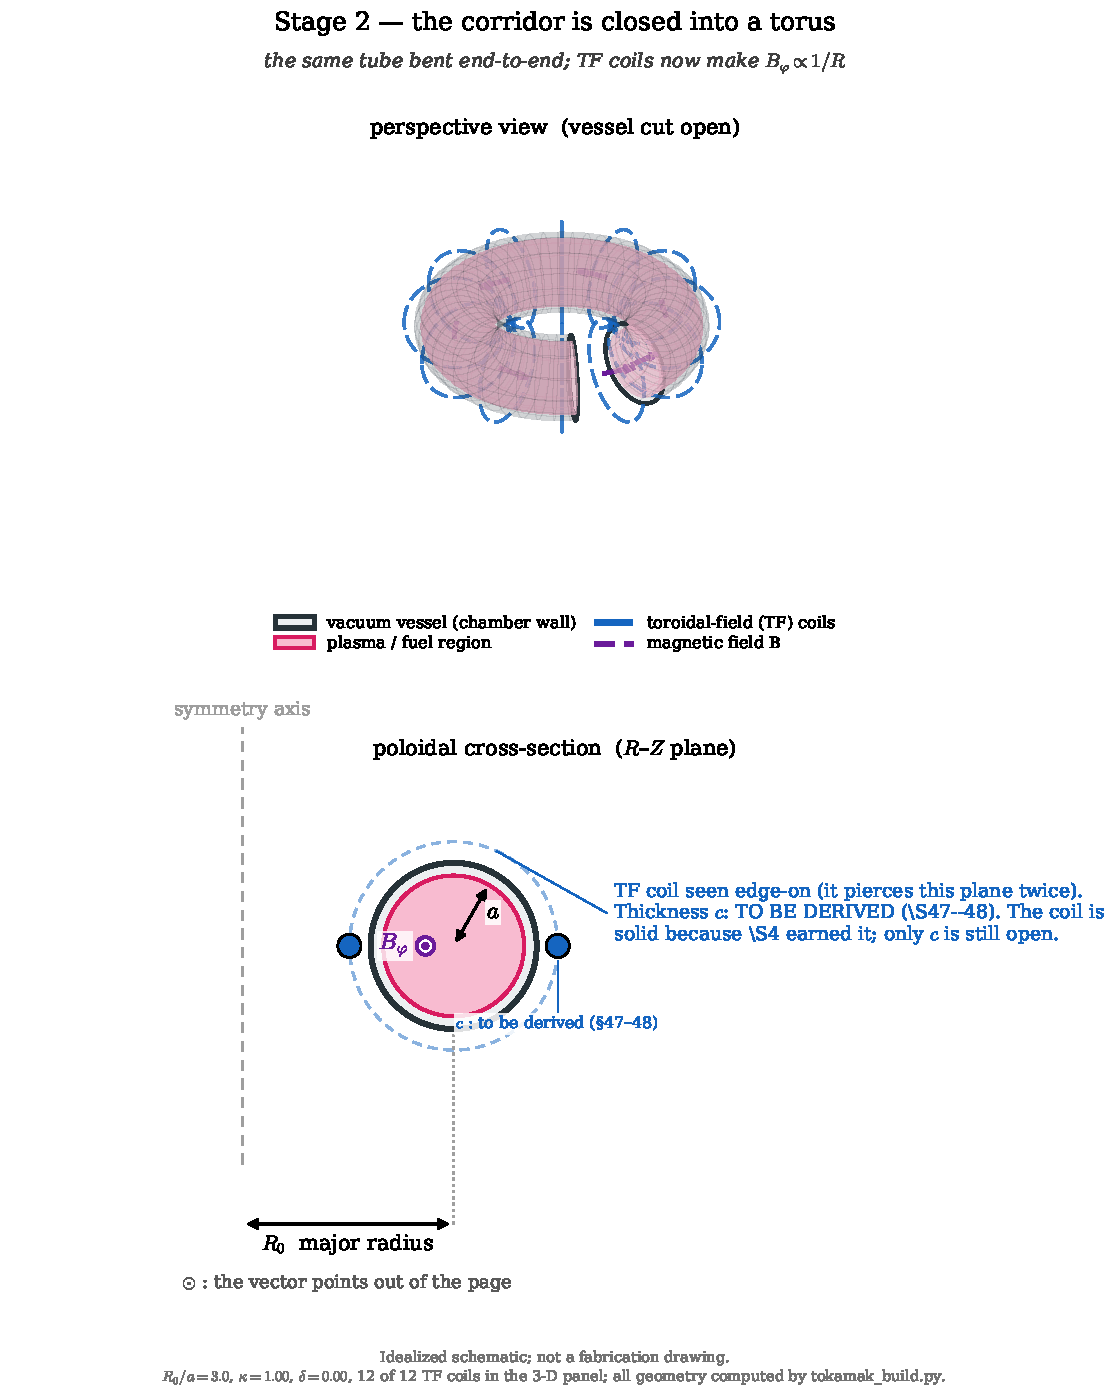
\includegraphics[width=1.0\textwidth]{figures/final/figM2_stage2_tall.pdf}
  \caption{The corridor closed into a torus. The straight solenoid turns have become toroidal-field coils around the same tube; $R_0$, $a$ and $B_\varphi$ now exist because the geometry acquired two lengths.}
  \label{fig:figM2_stage2_tall}
\end{figure}

% ============================== PAGE 5 ==============================
\section*{5. The closed bottle still leaks: toroidal drifts}

The gyro-orbit derivation assumed uniform $\mathbf B$. Equation~\eqref{eq:btor} makes the field
stronger on one side of every orbit than the other, and the field line itself is curved.
We now calculate the leading effect, assuming $r_L/R_0\ll1$ so the field changes little
during one gyro-orbit.

First derive a useful general result. Add a constant force $\mathbf F\perp\mathbf B$ to
Eq.~\eqref{eq:lorentz}, with $\mathbf E=0$. Seek a solution consisting of gyromotion plus a constant
velocity $\mathbf v_F$. Requiring the constant terms to cancel gives
\begin{equation}
 q\mathbf v_F\times\mathbf B+\mathbf F=0
 \quad\Longrightarrow\quad
 \boxed{\mathbf v_F=\frac{\mathbf F\times\mathbf B}{qB^2}}.
\label{eq:forcedrift}
\end{equation}
The torus supplies two effective forces. Conservation of the magnetic moment
$\mu=m v_\perp^2/(2B)$ is not merely asserted: a gyro-orbit is a current loop, so
\[
 \mu=\left(\frac{q\omega_c}{2\pi}\right)(\pi r_L^2)
 =\frac{m v_\perp^2}{2B}.
\]
When $B$ changes little during one orbit, gyro-averaging makes $\mu$ an adiabatic
invariant; the orbit therefore has potential energy $\mu B$ and gradient force
$\mathbf F_{\nabla B}=-\mu\nabla B$.\footnote{A systematic open derivation of
guiding-centre motion and its ordering assumptions is A. J. Brizard and T. S. Hahm,
``Foundations of nonlinear gyrokinetic theory,'' \url{https://arxiv.org/abs/physics/0409119}.}
Following a field line curved with radius $R$
also requires centripetal acceleration; in the frame of the guiding centre this enters
as the outward curvature force
$\mathbf F_c=(m v_\parallel^2/R)\hat{\mathbf R}$.

For Eq.~\eqref{eq:btor}, $\nabla B=-(B/R)\hat{\mathbf R}$. Therefore both effective forces point
radially outward. With $\mathbf B=B\hat{\boldsymbol\varphi}$ and
$\hat{\mathbf R}\times\hat{\boldsymbol\varphi}=\hat{\mathbf Z}$, Eq.~\eqref{eq:forcedrift} gives
\begin{equation}
\begin{aligned}
 \mathbf v_{\nabla B}
 &=\frac{m v_\perp^2}{2qBR}\,\hat{\mathbf Z},\\
 \mathbf v_c
 &=\frac{m v_\parallel^2}{qBR}\,\hat{\mathbf Z},\\[-2pt]
 \therefore\qquad
 \boxed{\mathbf v_d
 =\frac{m}{qBR}\left(v_\parallel^2+\frac12v_\perp^2\right)
 \hat{\mathbf Z}}.
\end{aligned}
\label{eq:toroidaldrift}
\end{equation}

Equation~\eqref{eq:toroidaldrift} is fatal to the design in its present form. Positive and negative charges
drift in opposite vertical directions because the sign is set by $q$. The resulting
charge separation creates a vertical electric field. Returning to Eq.~\eqref{eq:lorentz}, an electric
force $q\mathbf E$ inserted into Eq.~\eqref{eq:forcedrift} gives
\begin{equation}
 \mathbf v_E=\frac{\mathbf E\times\mathbf B}{B^2},
\label{eq:exb}
\end{equation}
which is independent of charge and mass. Ions and electrons now move together. For the
vertical charge-separation field produced here, that common drift is radially outward,
toward the vessel wall.

\designconsequence{Closing the straight field into a torus removes end loss but creates
systematic toroidal drifts. A purely toroidal magnetic field cannot confine the plasma.
The field line must be made to visit both the top and bottom of the torus so that the
same vertical drift alternates between outward and inward displacement.}

\newpage

% ============================== PAGE 6 ==============================
\section*{6. A second field is forced upon us}

A field line confined to one horizontal plane experiences the drift of Eq.~\eqref{eq:toroidaldrift} with the
same radial consequence throughout its journey. Make the line wind the short way around
the tube as well as the long way around the torus. It then passes successively through
the top and bottom of the cross-section; a vertical displacement is outward on one half
and inward on the other. The unbounded drift is replaced, to leading order, by a bounded
orbit excursion.

The required short-way field is called \emph{poloidal}. There are two broad ways to make
it. External helical windings can do so, producing a stellarator. The tokamak makes the
main poloidal field with a toroidal electric current carried by the plasma itself. On a
circular cross-section, apply Amp\`ere's law to a poloidal circle of radius $r$ enclosing
plasma current $I_{\rm enc}(r)$:
\begin{equation}
 2\pi r B_\theta(r)=\mu_0I_{\rm enc}(r),
 \qquad
 \boxed{B_\theta(r)=\frac{\mu_0I_{\rm enc}(r)}{2\pi r}}.
\label{eq:bpol}
\end{equation}
The combined field
\[
 \mathbf B=B_\varphi\hat{\boldsymbol\varphi}+B_\theta\hat{\boldsymbol\theta}
\]
is helical. A field line no longer remains at one height. The toroidal drift problem has
dictated a plasma current, and the plasma current has dictated a helical field.

Where does that current come from? Place a solenoid through the central hole and vary
its magnetic flux. Faraday's law,
\begin{equation}
 \oint\mathbf E\cdot d\boldsymbol\ell=-\frac{d\Phi}{dt},
\label{eq:faraday}
\end{equation}
creates a toroidal electric field. The plasma acts as the one-turn secondary winding of
a transformer; the induced electric field drives $I_p$. The central solenoid has therefore
not been added because tokamaks traditionally possess one. It has been demanded by the
decision to obtain the poloidal field through plasma current.

\begin{center}
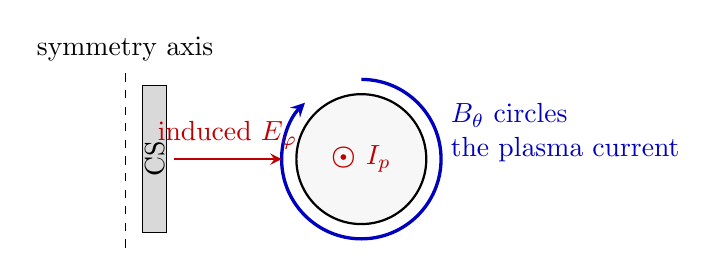
\begin{tikzpicture}[scale=0.75,>=stealth]
  \draw[dashed] (0,-1.5) -- (0,1.5) node[above]{symmetry axis};
  \draw[fill=black!15] (0.30,-1.25) rectangle (0.70,1.25);
  \node[rotate=90] at (0.50,0) {CS};
  \draw[thick,fill=black!3] (4,0) circle (1.10);
  \node[red!75!black] at (4,0) {$\boldsymbol\odot\ I_p$};
  \draw[blue!75!black,->,very thick] (4,1.35) arc[start angle=90,end angle=-225,
    radius=1.35];
  \node[right,blue!75!black,align=left] at (5.35,0.45) {$B_\theta$ circles\\the plasma current};
  \draw[red!75!black,->,thick] (0.82,0) -- (2.65,0)
    node[midway,above] {induced $E_\varphi$};
\end{tikzpicture}
\end{center}

\designconsequence{The machine revealed so far contains a vacuum vessel, toroidal-field
coils, a toroidal plasma, and a means of driving plasma current. This is the minimal
physical chain that creates the tokamak field. It is not yet a reactor: we have not shown
pressure equilibrium, stability, adequate confinement time, heating, exhaust, breeding,
magnet survival, or net electricity. Each of those failures will demand its own component.}

One distinction will matter later. The plasma current produces the principal poloidal
field that makes field lines helical. Separate external poloidal-field coils will be
introduced only when radial force balance, position control, and shaping require them.
The next derived parameter will be the pitch of the helix---the safety factor $q$---because
the current that repairs drift also creates the machine's first major stability limit.

\newpage


\begin{figure}[htbp]\centering
  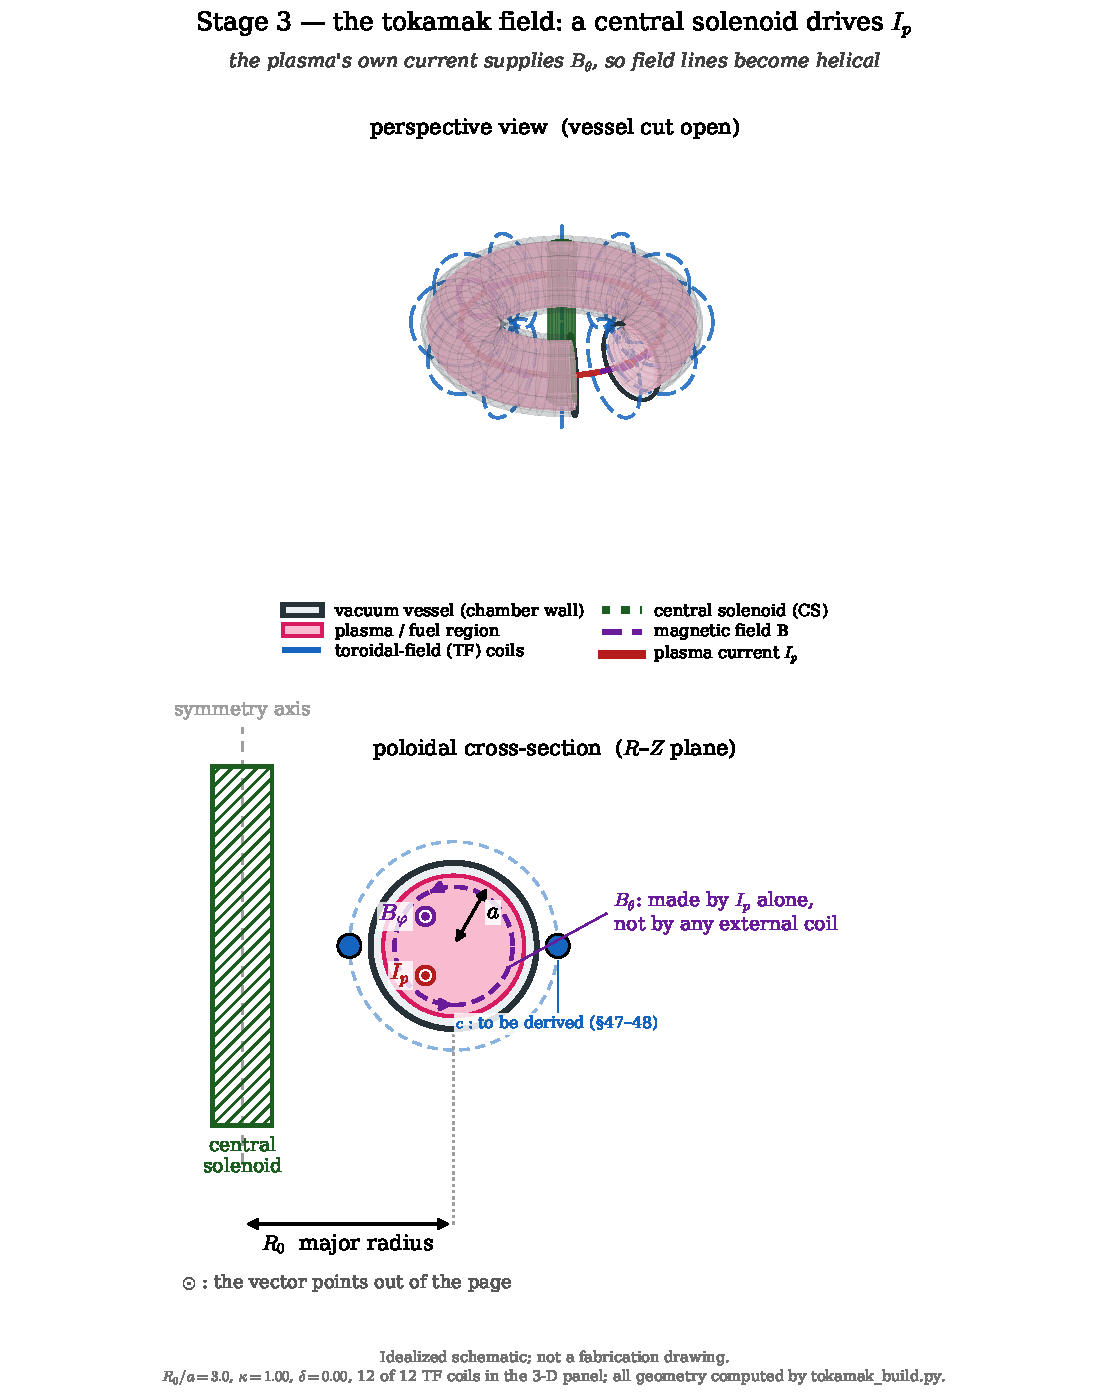
\includegraphics[width=1.0\textwidth]{figures/final/figM3_stage3_tall.pdf}
  \caption{The tokamak field. A central solenoid drives $I_p$, and $I_p$ alone supplies $B_\theta$ --- no external coil does this. Every component of the previous state is retained.}
  \label{fig:figM3_stage3_tall}
\end{figure}

% ============================== PAGE 7 ==============================
\section*{7. The helix has a pitch: the safety factor $q$}

The combined field has two components, so a field line advances two ways at once. On a
nearly circular magnetic surface of minor radius $r$, a short displacement has toroidal
length $R\,d\varphi$ and poloidal length $r\,d\theta$. Because the displacement is
parallel to $\mathbf B$, their ratio must equal the corresponding ratio of field
components:
\begin{equation}
 \frac{R\,d\varphi}{r\,d\theta}=\frac{B_\varphi}{B_\theta}.
\label{eq:pitch}
\end{equation}
At large aspect ratio the variation of $R$ and $B_\varphi$ around one cross-section is
small enough that $R\simeq R_0$ and $B_\varphi\simeq B_0$. One poloidal circuit,
$\Delta\theta=2\pi$, then advances the field line toroidally by $2\pi q$, where
\begin{equation}
 q(r)\equiv\frac{\Delta\varphi}{2\pi}
 \simeq \frac{rB_0}{R_0B_\theta(r)}.
\label{eq:qdef}
\end{equation}
Thus $q$ is simply the number of long-way circuits made per one short-way circuit. The
word \emph{safety} is historical; the stability reason for that name comes later.

\begin{center}
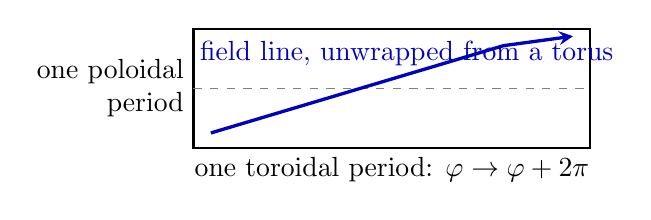
\begin{tikzpicture}[scale=0.63,>=stealth]
  \draw[thick] (0,0) rectangle (8,2.4);
  \draw[gray,dashed] (0,1.20)--(8,1.20);
  \draw[blue!75!black,very thick,->] (0.35,0.30) -- (3.30,1.18)
    -- (6.25,2.06) -- (7.65,2.25);
  \node[below] at (4,0) {one toroidal period: $\varphi\to\varphi+2\pi$};
  \node[left,align=right] at (0,1.20) {one poloidal\\period};
  \node[blue!75!black,above] at (4.3,1.45) {field line, unwrapped from a torus};
\end{tikzpicture}
\end{center}

Substitute the poloidal field already derived in Eq.~\eqref{eq:bpol}:
\begin{equation}
 q(r)\simeq\frac{2\pi r^2B_0}{\mu_0R_0I_{\rm enc}(r)},
 \qquad
 q_a\simeq\frac{2\pi a^2B_0}{\mu_0R_0I_p}.
\label{eq:qedge}
\end{equation}
The edge value $q_a$ has not been chosen by a convention. It has emerged from geometry,
Amp\`ere's law, and the decision to use plasma current for the poloidal field. Reading
the same relation backwards gives the equally important current relation
\begin{equation}
 I_p\simeq\frac{2\pi a^2B_0}{\mu_0R_0q_a}.
\label{eq:ipq}
\end{equation}
Any later lower bound on $q_a$ is therefore an upper bound on plasma current. This
connection is one of the load-bearing constraints in the later reactor audit.

A rational value $q=m/n$, for integers $m,n$, closes after $n$ poloidal and $m$
toroidal turns. An irrational value never exactly closes and instead samples its surface.

\designconsequence{The toroidal field, the plasma current, the size of the torus, and
the helix pitch are not independent knobs. Equation~\eqref{eq:ipq} ties them together.
The current that makes confinement possible has already spent part of the machine's
future stability budget.}

{\footnotesize The shaped generalization and later stability use are given by
Freidberg, Mangiarotti, and Minervini (2015), Eq.~(30):
\url{https://library.psfc.mit.edu/catalog/reports/2010/15ja/15ja021/15ja021_full.pdf}.}

\newpage

% ============================== PAGE 8 ==============================
\section*{8. A hot plasma is not a passenger: it has pressure}

Until now we have followed one particle in fields prescribed from outside. A fusion
plasma contains enough particles that its collective push matters. For one ideal gas
species, random impacts transfer momentum to a surface and give $p=nk_BT$. We are
using energy units for temperature, so this is simply $p=nT$. Electrons and ions each
contribute; quasineutrality gives $n_e\simeq n_i\equiv n$, hence
\begin{equation}
 p=n_eT_e+n_iT_i\simeq 2nT
 \quad\text{when }T_e\simeq T_i\equiv T.
\label{eq:pressure}
\end{equation}
For orientation, $n=10^{20}\,\mathrm{m^{-3}}$ and $T=10\,\mathrm{keV}$ give
$p\simeq3.2\times10^5\,\mathrm{Pa}$, about three atmospheres. This pressure is
inside a near-vacuum vessel, so it tries to expand the plasma.

At scales large compared with a gyro-orbit, it is useful to average the particles into
one conducting fluid. Its momentum equation is
\begin{equation}
 \rho\frac{d\mathbf v}{dt}=-\nabla p+\mathbf J\times\mathbf B.
\label{eq:mhdmomentum}
\end{equation}
Here $-\nabla p$ is the force due to pressure and $\mathbf J\times\mathbf B$ is the
magnetic force density. A static equilibrium requires
\begin{equation}
 \boxed{\mathbf J\times\mathbf B=\nabla p.}
\label{eq:forcebalance}
\end{equation}
This is a model declaration, not a universal law: it assumes slow evolution, negligible
bulk flow, small gyro-orbits compared with the plasma size, and an approximately scalar
pressure. Those assumptions will be checked rather than silently inherited when we use
the equation quantitatively.

One consequence follows without solving anything. Dot Eq.~\eqref{eq:forcebalance}
with $\mathbf B$:
\begin{equation}
 \mathbf B\cdot\nabla p
 =\mathbf B\cdot(\mathbf J\times\mathbf B)=0.
\label{eq:pressurefieldline}
\end{equation}
Pressure is constant along a field line. The invisible wall is therefore not a loose
collection of lines: a static confined plasma requires nested magnetic surfaces on
which pressure can live.

There is a natural way to compare plasma push with magnetic capability. Build the field
of a solenoid slowly. With $N$ turns, length $L$, area $A$, and flux linkage $NBA$,
the source supplies $dW=I\,d(NBA)$. Since $B=\mu_0NI/L$, integration gives
\begin{equation}
 W=\frac{B^2}{2\mu_0}AL.
\label{eq:fieldenergy}
\end{equation}
Thus $B^2/(2\mu_0)$ is the magnetic energy per unit volume and has the same units as
pressure. Define
\begin{equation}
 \boxed{\beta\equiv\frac{p}{B^2/(2\mu_0)}.}
\label{eq:beta}
\end{equation}
It is the fraction of magnetic pressure-scale that the plasma is asking the field to
hold. Raising $B$ makes a given pressure easier to support; raising $p$ makes the same
magnet work harder.

\designconsequence{A tokamak cannot be designed by field-line geometry alone. Its
magnetic surfaces must also balance pressure. This forces a second task on the coil
system: hold the plasma at a chosen radial position while its own pressure and current
try to move it.}

\vfill
{\footnotesize The static-MHD model and the use of $\beta$ in reactor design are treated
in the open Freidberg--Mangiarotti--Minervini manuscript cited on page~1. The field
energy relation above is derived from the work needed to establish a solenoidal field.}

\newpage

% ============================== PAGE 9 ==============================
\section*{9. Holding position forces external poloidal-field coils}

The plasma current is a toroidal current loop. A current loop in a vertical magnetic
field feels a radial force. This is not a slogan; apply the elementary force law
$d\mathbf F=I\,d\boldsymbol\ell\times\mathbf B$ to a circular loop. For
$d\boldsymbol\ell=R_0d\varphi\,\hat{\boldsymbol\varphi}$ and
$\mathbf B_v=B_v\hat{\mathbf Z}$,
\begin{equation}
 d\mathbf F=I_pR_0B_vd\varphi\,\hat{\mathbf R},
 \qquad
 \mathbf F_R=2\pi R_0I_pB_v\,\hat{\mathbf R}.
\label{eq:ringforce}
\end{equation}
Changing the sign of $B_v$ changes the force from outward to inward.

\begin{center}
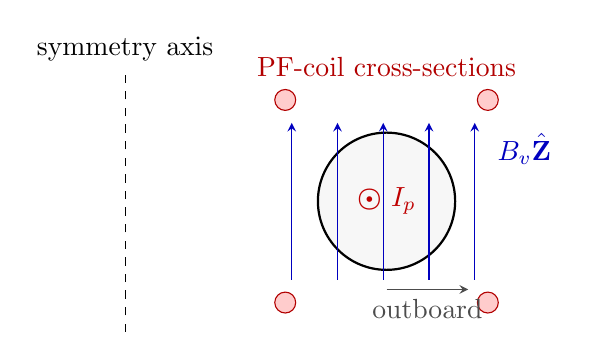
\begin{tikzpicture}[scale=0.83,>=stealth]
  \draw[dashed] (0,-2.0)--(0,2.0) node[above]{symmetry axis};
  \foreach \x/\y in {2.45/1.55,5.55/1.55,2.45/-1.55,5.55/-1.55}{
    \draw[red!70!black,fill=red!20] (\x,\y) circle (0.16);
  }
  \node[red!70!black] at (4.0,2.05) {PF-coil cross-sections};
  \draw[thick,fill=black!3] (4,0) circle (1.05);
  \node[red!75!black] at (4,0) {$\boldsymbol\odot\ I_p$};
  \foreach \x in {2.55,3.25,...,5.45}{
    \draw[blue!75!black,->] (\x,-1.20)--(\x,1.20);
  }
  \node[blue!75!black,right] at (5.55,0.80) {$B_v\hat{\mathbf Z}$};
  \draw[->,black!70] (4,-1.35)--(5.25,-1.35) node[midway,below] {outboard};
\end{tikzpicture}
\end{center}

The plasma has several sources of radial imbalance: its pressure is higher in the
interior; its own poloidal field has a curved, toroidal geometry; and the applied
toroidal field varies as $1/R$. Equation~\eqref{eq:forcebalance} says that the sum
must cancel, but it does \emph{not} say that a free current ring automatically sits
at the desired $R_0$. Equation~\eqref{eq:ringforce} gives the actuator that can
correct the residual force.

This finally distinguishes two uses of a poloidal field. The field generated by
$I_p$ is the principal field that makes field lines helical and repairs drift. The
external vertical component shown here is part of an applied \emph{poloidal-field}
(PF) system. Its first job is equilibrium and radial position. The same system will
later acquire separate coils for shaping and fast feedback.

We deliberately do not yet quote one ``required vertical field'' formula. Its exact
coefficient depends on the pressure profile, current profile, cross-section, and the
plasma's self-inductance. Giving a single number before those objects have been derived
would conceal those assumptions. At this stage physics has rigorously forced the
existence and the direction of the control field; the full equilibrium calculation will
set its magnitude.

\designconsequence{The first coils around the torus made $B_\varphi$. The central
solenoid drove $I_p$. Pressure balance now forces a separate external PF-coil system:
it must hold the plasma's position rather than merely create field lines.}

\newpage


\begin{figure}[htbp]\centering
  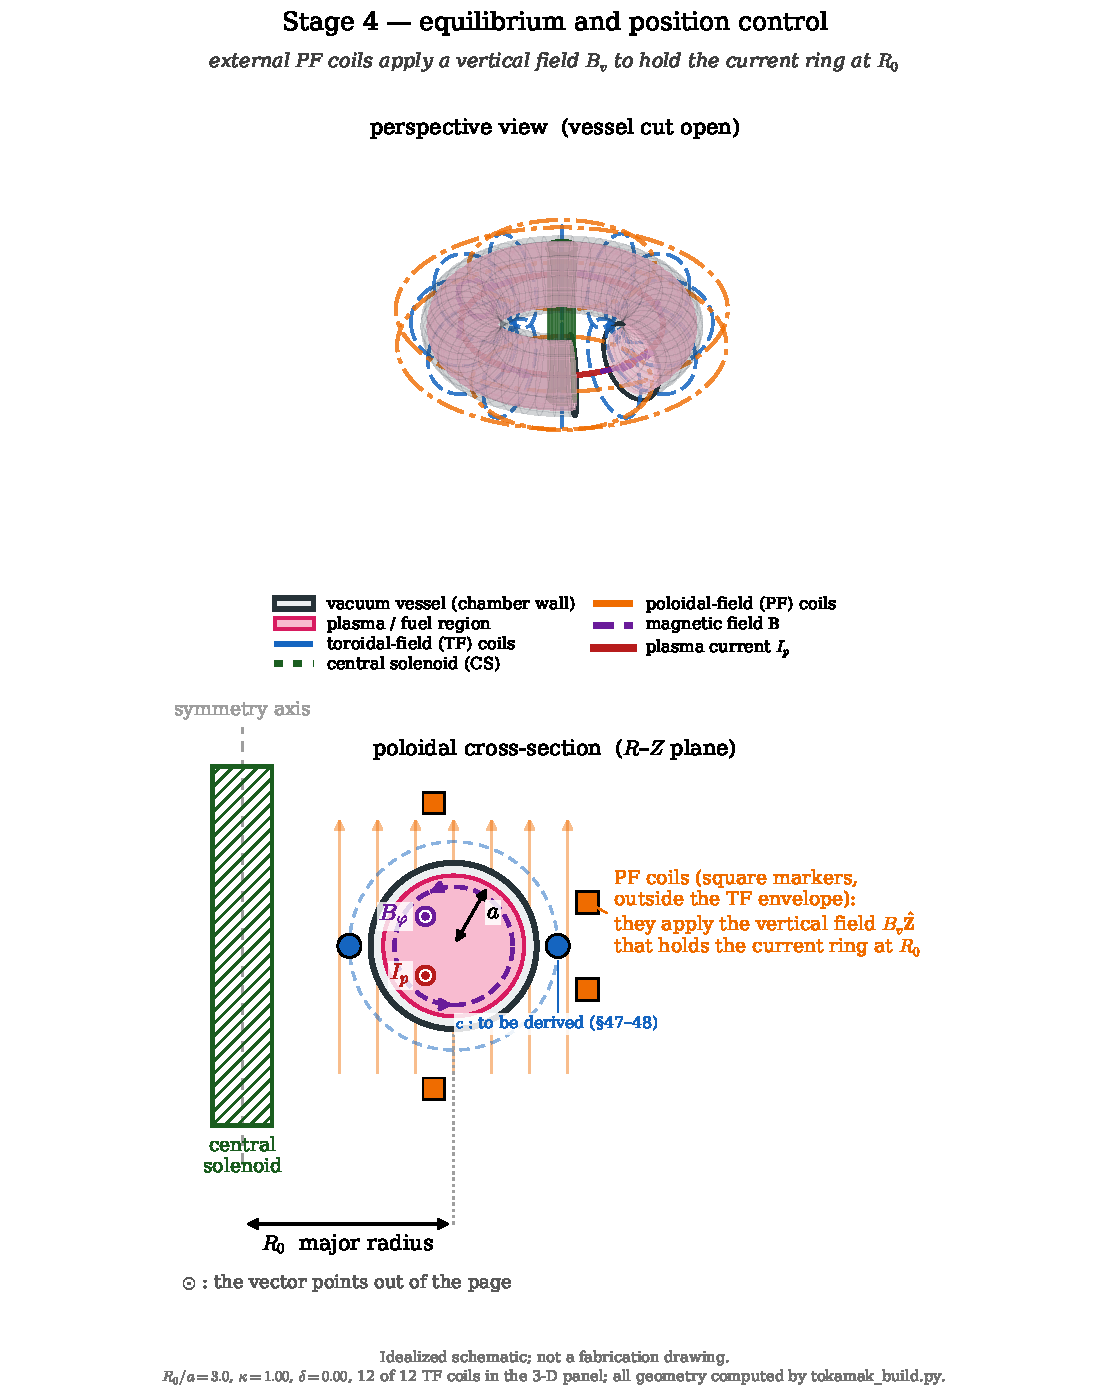
\includegraphics[width=1.0\textwidth]{figures/final/figM4_stage4_tall.pdf}
  \caption{Equilibrium and position control. External PF coils, drawn as square markers strictly outside the toroidal-field envelope, apply the vertical field that holds the current ring at $R_0$.}
  \label{fig:figM4_stage4_tall}
\end{figure}

% ============================== PAGE 10 ==============================
\section*{10. Flux surfaces turn coil currents into a plasma boundary}

To say that coils ``hold position'' is still too vague. Axisymmetry lets us name the
geometric object they control. In cylindrical coordinates $(R,\varphi,Z)$, with no
$\varphi$ dependence, $\nabla\cdot\mathbf B=0$ becomes
\begin{equation}
 \frac{\partial(RB_R)}{\partial R}+\frac{\partial(RB_Z)}{\partial Z}=0.
\label{eq:divfree}
\end{equation}
This is the two-dimensional statement that a flow has no sources or sinks. Therefore
there is a scalar function $\psi(R,Z)$ whose derivatives generate the poloidal field:
\begin{equation}
 B_R=-\frac1R\frac{\partial\psi}{\partial Z},\qquad
 B_Z=\frac1R\frac{\partial\psi}{\partial R},\qquad
 \mathbf B_p=\frac{\nabla\psi\times\hat{\boldsymbol\varphi}}{R}.
\label{eq:psidef}
\end{equation}
Substituting these two derivatives into Eq.~\eqref{eq:divfree} verifies the claim in
one line. More importantly,
\begin{equation}
 \mathbf B\cdot\nabla\psi=0.
\label{eq:psiconstant}
\end{equation}
The toroidal part is also perpendicular to $\nabla\psi$ because $\psi$ does not
depend on $\varphi$. Thus a field line stays on a surface $\psi=\text{constant}$.
The quantity $2\pi\psi$ is the poloidal magnetic flux enclosed by the toroidal loop
at $(R,Z)$.

\begin{center}
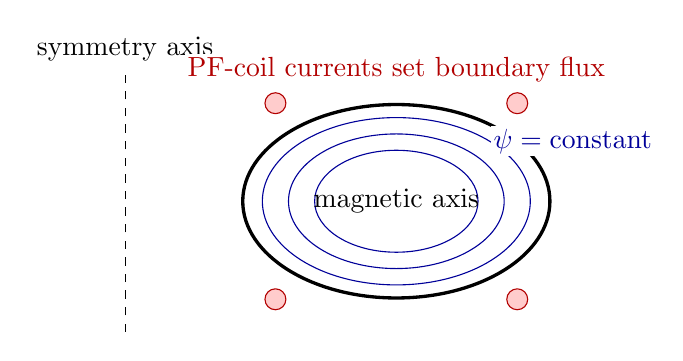
\begin{tikzpicture}[scale=0.83,>=stealth]
  \draw[dashed] (0,-2.0)--(0,2.0) node[above]{symmetry axis};
  \foreach \rx/\ry in {1.25/0.78,1.65/1.03,2.05/1.28}{
    \draw[blue!60!black] (4.15,0) ellipse [x radius=\rx,y radius=\ry];
  }
  \draw[very thick] (4.15,0) ellipse (2.35 and 1.48);
  \node at (4.15,0) {magnetic axis};
  \node[blue!60!black,fill=white,inner sep=1pt] at (6.85,0.92) {$\psi=\mathrm{constant}$};
  \foreach \x/\y in {2.30/1.50,6.00/1.50,2.30/-1.50,6.00/-1.50}{
    \draw[red!70!black,fill=red!20] (\x,\y) circle (0.16);
  }
  \node[red!70!black,fill=white,inner sep=1pt] at (4.15,2.02) {PF-coil currents set boundary flux};
\end{tikzpicture}
\end{center}

The outer closed contour is not just the vessel wall. It is the last closed magnetic
surface selected by the plasma current together with the PF-coil currents. The vessel
must contain and protect this arrangement, but it cannot replace the magnetic boundary:
a conducting wall cannot hold a $10\,\mathrm{keV}$ plasma in steady contact.

This is also why shape will matter. Moving PF-coil currents changes the boundary value
of $\psi$, and therefore changes the cross-section of the nested surfaces. A circle is
only the first solvable shape, not a physical law. Elongation and triangularity will be
introduced only when a specific performance or stability problem demands them.

\designconsequence{PF coils control flux, and flux contours are the plasma boundary.
The emerging machine therefore needs a vacuum vessel outside a deliberately shaped,
magnetically defined plasma---not a metal container that touches the fuel.}

\vfill
{\footnotesize This axisymmetric flux representation is derived from
$\nabla\cdot\mathbf B=0$ above. For an openly available full equilibrium treatment,
see Cerfon and Freidberg, ``One size fits all'' analytic solutions to the
Grad--Shafranov equation (2010), \href{https://www.researchgate.net/publication/234959741_One_size_fits_all_analytic_solutions_to_the_Grad-Shafranov_equation}{open public manuscript}.}

\newpage

% ============================== PAGE 11 ==============================
\section*{Eleven. The transformer has a clock}

The central solenoid was introduced to drive the toroidal current. Faraday's law now
reveals a price. Around a toroidal loop,
\begin{equation}
 V_{\rm loop}\equiv\oint\mathbf E\cdot d\boldsymbol\ell
 =-\frac{d\Phi_{\rm link}}{dt}.
\label{eq:loopvoltage}
\end{equation}
Integrating through a discharge gives
\begin{equation}
 \int V_{\rm loop}\,dt=-\Delta\Phi_{\rm link}.
\label{eq:voltseconds}
\end{equation}
The available linked-flux change has units of volt-seconds. A central solenoid can
only swing through a finite magnetic flux before its current, field, and mechanical
limits are reached. It can start and sustain a pulse, but it cannot supply a steady
DC loop voltage forever. A volt-second is exactly a weber:
$1\,\mathrm{V\,s}=1\,\mathrm{Wb}$. It is therefore a unit of linked magnetic
flux---the transformer's finite magnetic-flux budget---not a unit of stored energy.

The induced current initially supplies useful heat. The local electrical power density
is $\mathbf J\cdot\mathbf E$; integrating over the plasma gives
\begin{equation}
 P_{\rm ohm}=\int\mathbf J\cdot\mathbf E\,dV
 \simeq I_pV_{\rm loop}=I_p^2R_p.
\label{eq:ohmic}
\end{equation}
The final form is the lumped-circuit approximation, with plasma resistance $R_p$.
It is useful for the design argument, not a claim that the current density is uniform.

There is a second limit. In a fully ionized, collisional plasma the classical Spitzer
resistivity falls approximately as
\begin{equation}
 \eta\equiv\frac{E_\parallel}{J_\parallel}\propto T_e^{-3/2}.
\label{eq:spitzer}
\end{equation}
Hot electrons collide less effectively, so at comparable current density the plasma
becomes a better conductor and ohmic heating weakens. This is a pleasant fact for
current flow and an inconvenient fact for trying to heat a reactor plasma by resistance.

\begin{center}
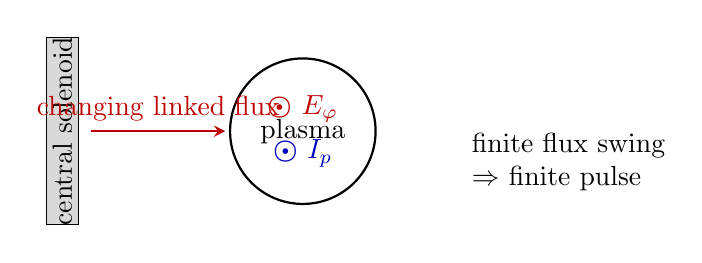
\begin{tikzpicture}[scale=0.88,>=stealth]
  \draw[fill=black!15] (0.0,-1.35) rectangle (0.46,1.35);
  \node[rotate=90] at (0.23,0) {central solenoid};
  \draw[thick] (3.7,0) circle (1.05);
  \node at (3.7,0) {plasma};
  \draw[red!75!black,->,thick] (0.65,0)--(2.58,0)
    node[midway,above] {changing linked flux};
  \node[red!75!black] at (3.7,0.32) {$\boldsymbol\odot\ E_\varphi$};
  \node[blue!75!black] at (3.7,-0.32) {$\boldsymbol\odot\ I_p$};
  \node[right,align=left] at (6.0,-0.45) {finite flux swing\\$\Rightarrow$ finite pulse};
\end{tikzpicture}
\end{center}

\designconsequence{The central solenoid has two jobs---start the plasma current and
provide early ohmic heat---but neither is an indefinitely scalable heat source. The
machine must acquire auxiliary heating, and eventually non-inductive current drive, if
it is to operate beyond a transformer pulse.}

\vfill
{\footnotesize The $T_e^{-3/2}$ Spitzer scaling and the power-density form
$\eta J^2$ are available openly in the NRL Plasma Formulary:
\url{https://www.nrl.navy.mil/Portals/38/PDF%20Files/NRL_Plasma_Formulary_2019.pdf}.}

\newpage

% ============================== PAGE 12 ==============================
\section*{12. Reaching fusion temperature forces a heating system}

The statement ``make the fuel hot'' on page~1 can now be made into an energy balance.
Each Maxwellian species has thermal energy density $3n_sT_s/2$. For an approximately
uniform D--T plasma with equal ion and electron temperatures,
\begin{equation}
 W\simeq 3nTV,
 \qquad
 P_{\rm loss}\equiv\frac{W}{\tau_E}.
\label{eq:taue}
\end{equation}
The first relation is energy stored in the plasma. The second \emph{defines} the
energy-confinement time $\tau_E$: if all heating were removed, it is the time scale on
which the stored energy would be lost at the present loss rate.

The bookkeeping law is therefore
\begin{equation}
 \frac{dW}{dt}=P_{\rm aux}+P_\alpha-P_{\rm loss}-P_{\rm rad}.
\label{eq:powerbalance}
\end{equation}
At startup $P_\alpha$ is small because fusion is small. Auxiliary power must raise
$W$ faster than transport and radiation remove it. Later, the $3.5\,\mathrm{MeV}$
alpha particles from Eq.~\eqref{eq:dt} are charged and can be magnetically confined;
their deposited energy is the desired self-heating term $P_\alpha$. The $14.1\,\mathrm{MeV}$
neutrons are neutral and escape, eventually to be captured in a blanket.

Why not simply fire charged particles into the plasma? The same magnetic field that
confines the fuel bends an incoming charged beam before it reaches the core. A neutral
beam solves that entry problem: neutral atoms cross the field, ionize in the plasma,
and then transfer their energy and momentum by collisions. Radio-frequency systems use
another handle already present in Eq.~\eqref{eq:lorentz}: an oscillating electric field
can transfer energy resonantly to selected charged-particle orbits. These are not
ornaments on a completed tokamak. They are responses to the transformer and power-balance
limits just derived.

\begin{center}
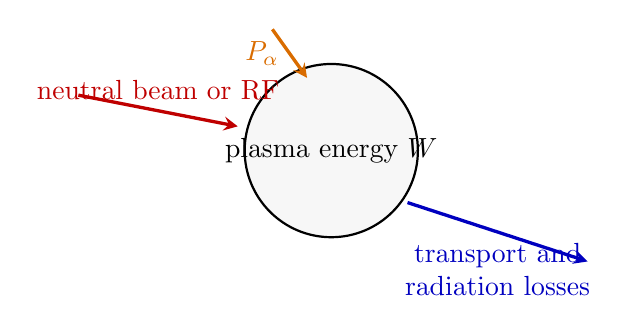
\begin{tikzpicture}[scale=0.88,>=stealth]
  \draw[thick,fill=black!3] (4,0) circle (1.25);
  \node at (4,0) {plasma energy $W$};
  \draw[red!75!black,->,very thick] (0.35,0.8)--(2.65,0.35)
    node[midway,above,align=center] {neutral beam or RF};
  \draw[orange!85!black,->,very thick] (3.15,1.75)--(3.65,1.05)
    node[midway,left] {$P_\alpha$};
  \draw[blue!75!black,->,very thick] (5.1,-0.75)--(7.7,-1.6)
    node[midway,below,align=center] {transport and\\radiation losses};
\end{tikzpicture}
\end{center}

The next question is not yet whether the machine makes net electricity. It is more
basic: how much pressure can a magnetic equilibrium and a stable plasma sustain, and
how should the boundary be shaped to improve that answer? Those questions will force
elongation, triangularity, feedback, and the first genuine stability limits. Only after
the ordinary tokamak has been derived on those terms will it make sense to ask whether
a spherical tokamak changes the bargain.

\designconsequence{Twelve pages in, the machine has emerged component by component:
a vacuum environment, toroidal-field coils, a plasma current and central solenoid,
external PF coils, and auxiliary heating. What remains absent is just as important:
the shaped boundary, exhaust, blanket, shielding, superconducting magnets, and the
reactor's energy ledger must each earn their place through the next physical failure.}


\begin{figure}[htbp]\centering
  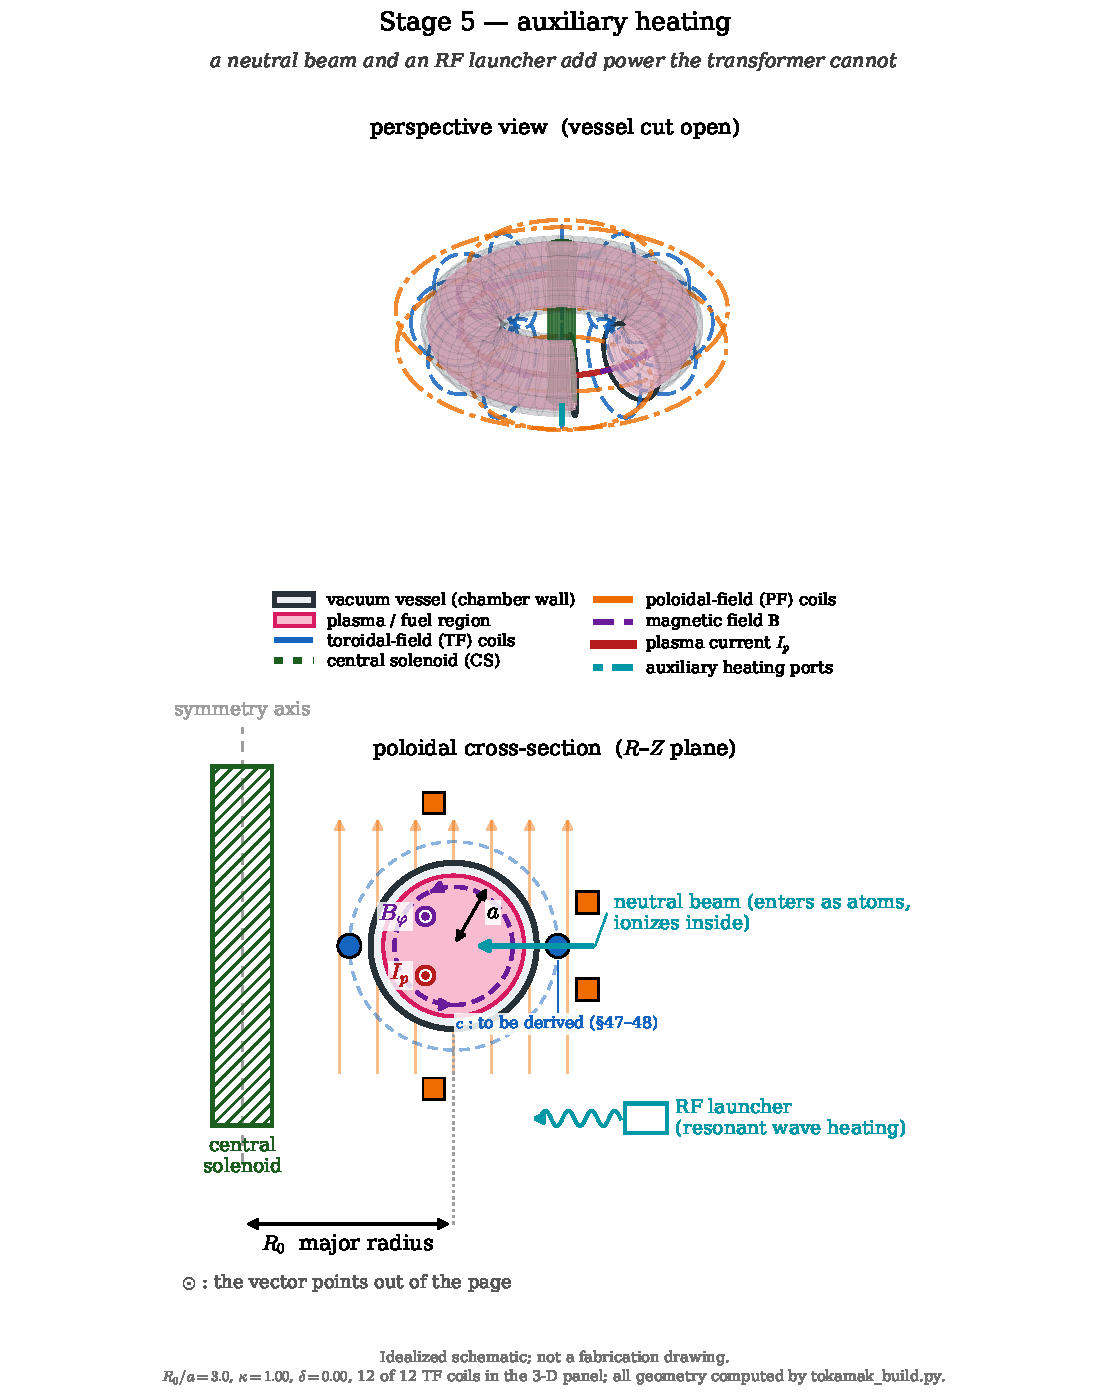
\includegraphics[width=1.0\textwidth]{figures/final/figM5_stage5_tall.pdf}
  \caption{Auxiliary heating. A tangential neutral beam and a radial RF launcher add the power the transformer cannot. No blanket, divertor or shield appears: none has been derived.}
  \label{fig:figM5_stage5_tall}
\end{figure}

% ============================= PAGE 13 ==============================
\newpage
\section*{13. More room is useful; a taller cross-section supplies it}

The circular cross-section used so far was deliberately austere. It makes the geometry
easy to see, but it is not the only allowed shape. Suppose the plasma boundary is an
ellipse with horizontal semi-axis $a$ and vertical semi-axis $\kappa a$. The dimensionless
number
\begin{equation}
 \kappa\equiv\frac{\hbox{vertical semi-axis}}{\hbox{horizontal semi-axis}}
 \label{eq:kappa}
\end{equation}
is called \emph{elongation}. A circle has $\kappa=1$; a vertically stretched plasma has
$\kappa>1$. Parameterize the boundary by
\[
 R(\theta)=R_0+a\cos\theta,\qquad Z(\theta)=\kappa a\sin\theta.
\]
The cross-sectional area is $\pi(\kappa a)a=\pi\kappa a^2$. Rotating that area once
around the major radius $R_0$ gives, to leading order in $a/R_0$,
\begin{equation}
 V=2\pi R_0\,(\pi\kappa a^2)=2\pi^2R_0a^2\kappa.
 \label{eq:elongated-volume}
\end{equation}
Thus, at fixed $R_0$ and $a$, elongation buys volume linearly. More volume can hold more
fuel and more fusion power; later we will state exactly which other quantities must be
held fixed before making that comparison.

\friedbergvariable{$\kappa$ (elongation)}{Equation~\eqref{eq:kappa} changes the plasma
volume in Eq.~\eqref{eq:elongated-volume} and enters the shaped safety-factor and current
limits derived below. It is not decorative geometry: it is a design lever with a
stability cost.}

The price is immediate. A round set of poloidal-field coils naturally supports a round
boundary. An elliptical boundary needs an intentionally nonuniform external field: some
coils pull or push more strongly above and below the midplane than at the outboard side.
The PF-coil system derived on page 9 therefore acquires a second job. It does not merely
keep the plasma centered; it helps choose the boundary shape. This is the first time an
earlier component has been asked to do more than solve the failure that first called it
into existence.

\imagebrief{Cumulative construction state 5: elongated conventional tokamak}{Use the
existing toroidal vacuum vessel, TF coils, central solenoid, plasma-current arrow, and
external PF coils. Change only the plasma cross-section from circular to vertically
elongated, label its semi-axes $a$ and $\kappa a$, and show that the upper/lower shaping
coils are part of the same PF system. This is a construction-state image, not a reset
physics sketch. Generate it reproducibly with the project figure workflow.}

\begin{figure}[htbp]\centering
  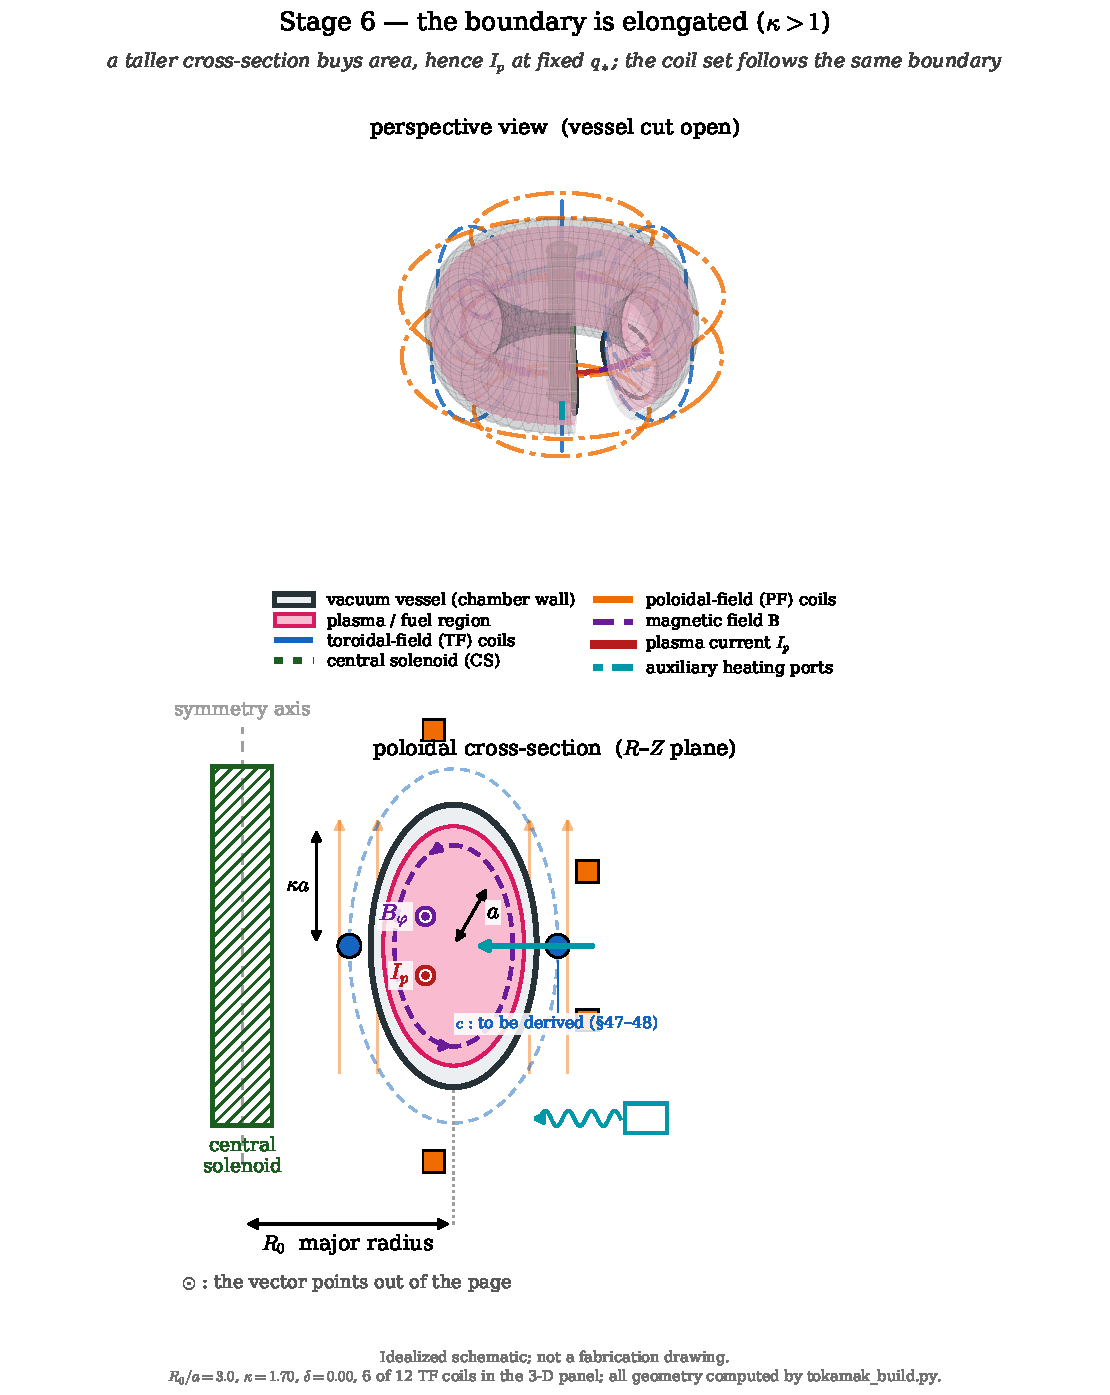
\includegraphics[width=1.0\textwidth]{figures/final/figM6_stage6_tall.pdf}
  \caption{Machine state: elongation. A taller cross-section supplies volume without growing every linear dimension, and the coil set follows the same boundary. Every component of the previous state is retained.}
  \label{fig:figM6_stage6_tall}
\end{figure}


\model{Equation~\eqref{eq:elongated-volume} treats the cross-section as an ellipse and
the torus as thin enough that its circumference is $2\pi R_0$. Real equilibria also use
triangularity and have shifted magnetic surfaces. Those refinements come only after the
basic geometric benefit and cost of $\kappa$ are clear.}

\designconsequence{If a reactor needs more plasma volume without simply increasing every
linear dimension, it has a reason to elongate the cross-section. That choice requires
shaping PF coils and raises a new question: is the taller plasma passively stable?}

% ============================= PAGE 14 ==============================
\newpage
\section*{14. A taller plasma can tip: shaping requires feedback}

Imagine displacing an elongated plasma a small distance $z$ upward. The magnetic forces
from the surrounding coils change. Near a chosen equilibrium height, any smooth vertical
force can be expanded as
\begin{equation}
 F_Z(z)=F_Z(0)+\left.\frac{\partial F_Z}{\partial z}\right|_0z+\cdots .
 \label{eq:vertical-linearization}
\end{equation}
At equilibrium $F_Z(0)=0$. Newton's law then becomes
\begin{equation}
 M\ddot z=K_z z,\qquad
 K_z\equiv\left.\frac{\partial F_Z}{\partial z}\right|_0 .
 \label{eq:vertical-mode}
\end{equation}
If $K_z<0$, Eq.~\eqref{eq:vertical-mode} is an oscillator: a displacement creates a
restoring force. If $K_z>0$, its solutions include $z\propto e^{\sqrt{K_z/M}t}$: a small
upward displacement grows instead of returning. This elementary sign test is the core
of a vertical instability. Elongation generally makes this control problem harder,
because a tall current-carrying column has a stronger tendency to move as a whole.

This does \emph{not} make elongation forbidden. It says that its equilibrium cannot be
trusted to remain in place by itself. A real machine measures its position with magnetic
sensors, compares it with a requested position, and changes currents in selected PF
coils. The control system must act before the growing displacement reaches the wall.
The causal chain is therefore precise: more useful shape $\rightarrow$ weaker passive
vertical stability $\rightarrow$ sensors, power supplies, and fast controlled coils.

\imagebrief{Cumulative construction state 5B: add the control loop}{Start with state 5.
Add small magnetic-position sensors outside the vessel, arrows from them to a controller
box, and arrows from the controller to two fast vertical-control PF coils. Draw a faint
displaced plasma outline and label it $+z$; keep all previously derived components
visible. The purpose is to show an engineering system forced by Eq.~\eqref{eq:vertical-mode},
not to imply that the controller itself is a magnetic component.}

\begin{figure}[htbp]\centering
  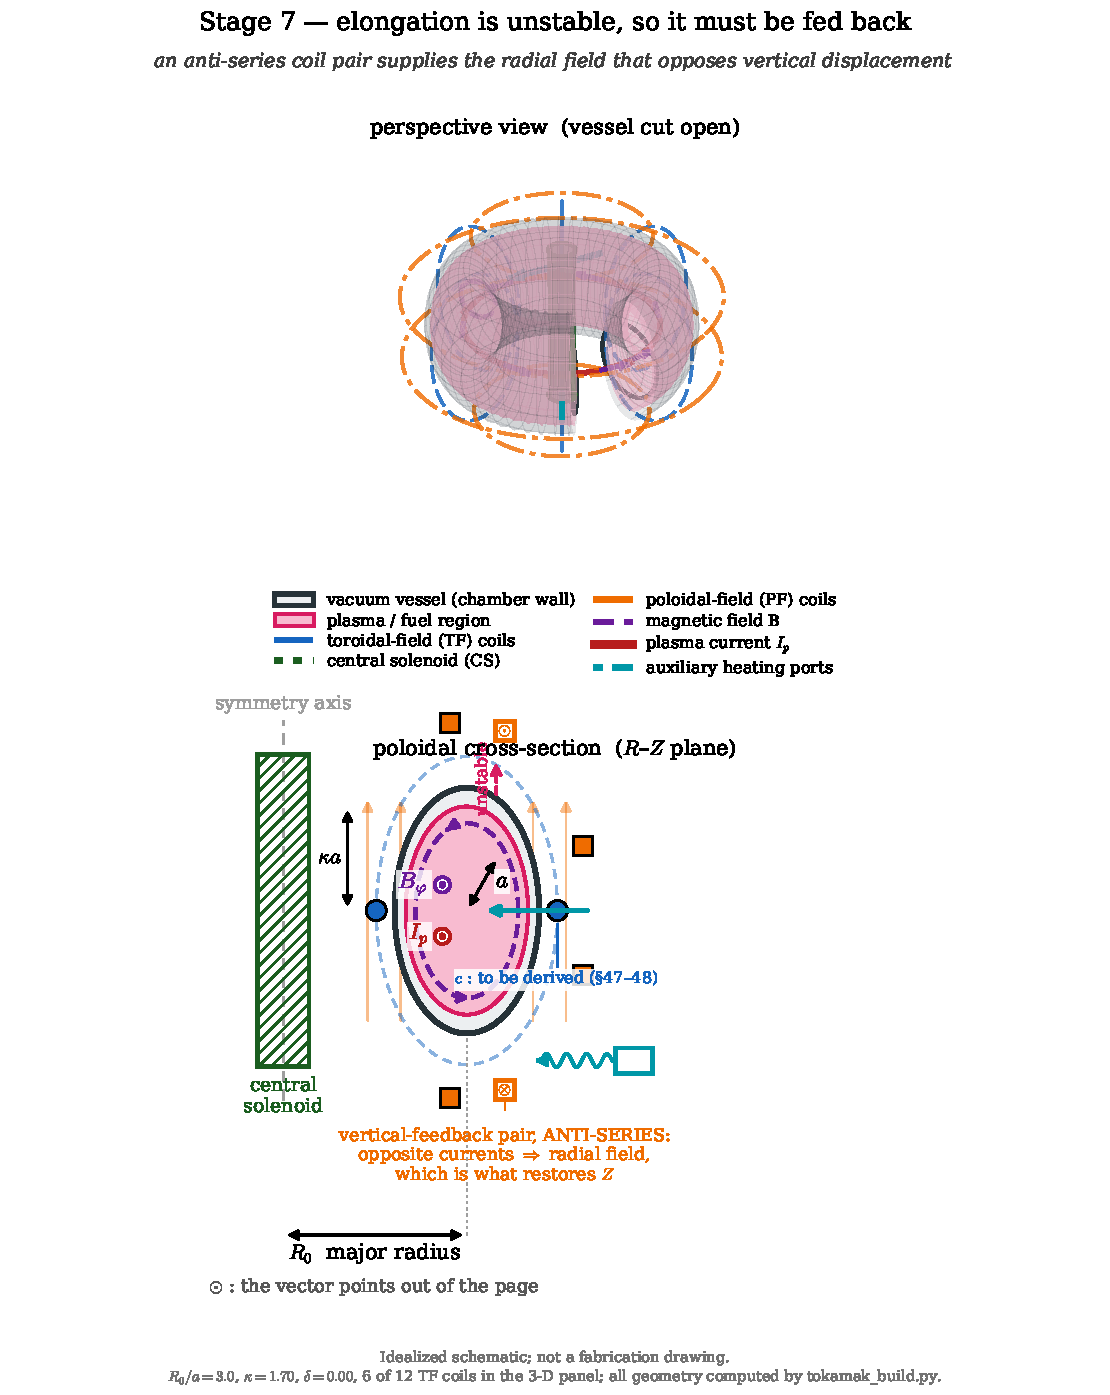
\includegraphics[width=1.0\textwidth]{figures/final/figM7_stage7_tall.pdf}
  \caption{Machine state: vertical control. The pair is wired \emph{anti-series} ($\odot$ above, $\otimes$ below): opposite currents make the combined field radial on the midplane, which is what restores $Z$. A same-sign pair would only move the plasma in $R$.}
  \label{fig:figM7_stage7_tall}
\end{figure}


\model{Equation~\eqref{eq:vertical-mode} is a one-coordinate linear model. Actual
vertical control couples plasma shape, conducting structures, coil circuits, and sensor
delays. It is used here only to establish the sign logic that makes feedback necessary.
For an openly available treatment of elongation and vertical stability, see E.~Cerfon,
J.~P.~Freidberg, and J.~P.~Vesey, ``Tokamak elongation: how much is too much? Part 1,''
\url{https://www.cambridge.org/core/services/aop-cambridge-core/content/view/1ABC7975053E19C0A93D9952CBB53102/S0022377815001270a.pdf}.}

\designconsequence{A shaped tokamak is not merely coils plus plasma. It includes a
closed feedback system. The allowed elongation is set jointly by the gain in volume,
the available PF-coil authority, nearby conducting structures, and the speed and
reliability of active control.}

% ============================= PAGE 15 ==============================
\newpage
\section*{15. The same geometry changes how much plasma current is allowed}

We already derived a safety factor for a simple circular plasma. It counted, in effect,
how far a field line moves toroidally while making one poloidal circuit. The local
version at minor radius $r$ is
\begin{equation}
 q(r)=\frac{2\pi r^2B_0}{\mu_0R_0 I_{\rm enc}(r)},
 \qquad
 I_{\rm enc}(r)=2\pi\int_0^r j_\varphi(r')r'\,dr'.
 \label{eq:qprofile}
\end{equation}
Here $j_\varphi$ is the toroidal current density and $I_{\rm enc}$ is the current inside
the selected magnetic surface. The first relation follows from the same field-line ratio
used before, $q\simeq rB_\varphi/(R_0B_\theta)$; the second is the area integral of
current density, and Amp\`ere's law gives $B_\theta\simeq\mu_0I_{\rm enc}/(2\pi r)$.

An elongated boundary alters this simple geometry. A widely used large-aspect-ratio,
elongated-plasma estimate is
\begin{equation}
 q_* = \frac{2\pi a^2B_0}{\mu_0R_0I_p}\,
       \frac{1+\kappa^2}{2}.
 \label{eq:qstar}
\end{equation}
The first fraction is the circular edge estimate. The factor $(1+\kappa^2)/2$ records
that one poloidal circuit is no longer circular. Equation~\eqref{eq:qstar} is not being
introduced as a mysterious correction: it is the next-order geometry that becomes
necessary once we deliberately choose $\kappa\ne1$.

For the simple global kink constraint used in the reactor-design model, require
$q_*>q_K$, where $q_K\simeq2$. Solving Eq.~\eqref{eq:qstar} for $I_p$ gives a current
ceiling,
\begin{equation}
 I_p < \frac{2\pi a^2B_0}{\mu_0R_0q_K}\,
        \frac{1+\kappa^2}{2}.
 \label{eq:ip-kink-limit}
\end{equation}
The direction of the result is instructive. More toroidal field $B_0$, more minor
cross-section, or more elongation permits more current under this particular limit;
larger major radius $R_0$ lowers the permitted current when the other variables are held
fixed.

\friedbergvariable{$q_*$ and $I_p$}{Equation~\eqref{eq:qstar} is the shaped global
safety factor used by Freidberg's reactor model. Equation~\eqref{eq:ip-kink-limit}
turns its stability requirement into a quantitative current constraint. Together they
couple geometry ($R_0,a,\kappa$), field ($B_0$), and the plasma current ($I_p$).}

\model{The estimate in Eq.~\eqref{eq:qstar}, and the $q_K\simeq2$ limit, are the
large-aspect-ratio design closure adopted in Freidberg, Mangiarotti, and Minervini
(2015), Eqs.~(30) and (39), open manuscript cited on page 1. A full stability boundary
depends on profiles, wall response, and feedback. We use the explicit model before
asking it to carry any design conclusion.}

\designconsequence{Elongation is valuable twice in this reduced model: it increases
volume and relaxes a particular current limit. But it also created the feedback demand
on the preceding page. A good parameter cannot be optimized one equation at a time.}

% ============================= PAGE 16 ==============================
\newpage
\section*{16. A single safety factor is not enough: the current profile matters}

Equation~\eqref{eq:qprofile} contains more information than the edge number $q_*$. If
two plasmas have the same total $I_p$ but different functions $j_\varphi(r)$, then
$I_{\rm enc}(r)$ and therefore $q(r)$ differ throughout the interior. The machine
cannot treat its current as a single knob when the plasma's magnetic geometry depends on
where that current flows.

The reason is already visible in the field-line picture. When $q=m/n$ for integers $m$
and $n$, a field line closes after $m$ poloidal and $n$ toroidal circuits in the idealized
description. Such rational surfaces are not automatically harmful, but perturbations
can accumulate coherently there. That is why later stability discussions specify a
\emph{profile} such as $q(0)$ and $q(a)$, rather than only a total current.

There is also a practical lesson. The transformer acts on current induction, while
auxiliary systems can add or reshape current through other mechanisms. The sources of
current and the resulting profile must both be accounted for in any steady-state claim.
At this stage we need not choose a detailed profile. We need to preserve the variable
that the later stability and bootstrap-current arguments will require.

Here bootstrap current means a pressure-gradient-driven share of the toroidal plasma
current. Its orbit-and-collision mechanism is derived on pages 36--37, before any
numerical bootstrap fraction is used.

\supportingquantity{$q(r)$ and $j_\varphi(r)$}{The radial safety-factor profile in
Eq.~\eqref{eq:qprofile} carries the current-distribution information that a single
$q_*$ loses. Later closure arguments will need it to distinguish total current from
the fraction supplied by the plasma itself or by external drive.}

\imagebrief{Cumulative construction state 6: shape and profile-control hardware}{Start
with the elongated, feedback-controlled machine. Add only a clear callout that the
central solenoid and auxiliary current-drive/heating ports influence the toroidal-current
profile $j_\varphi(r)$, alongside a small inset of nested flux surfaces labelled
$q(r)$. Do not draw a spherical tokamak or a finished power plant. This image should
make the distinction between total $I_p$ and profile $j_\varphi(r)$ legible.}

\begin{figure}[htbp]\centering
  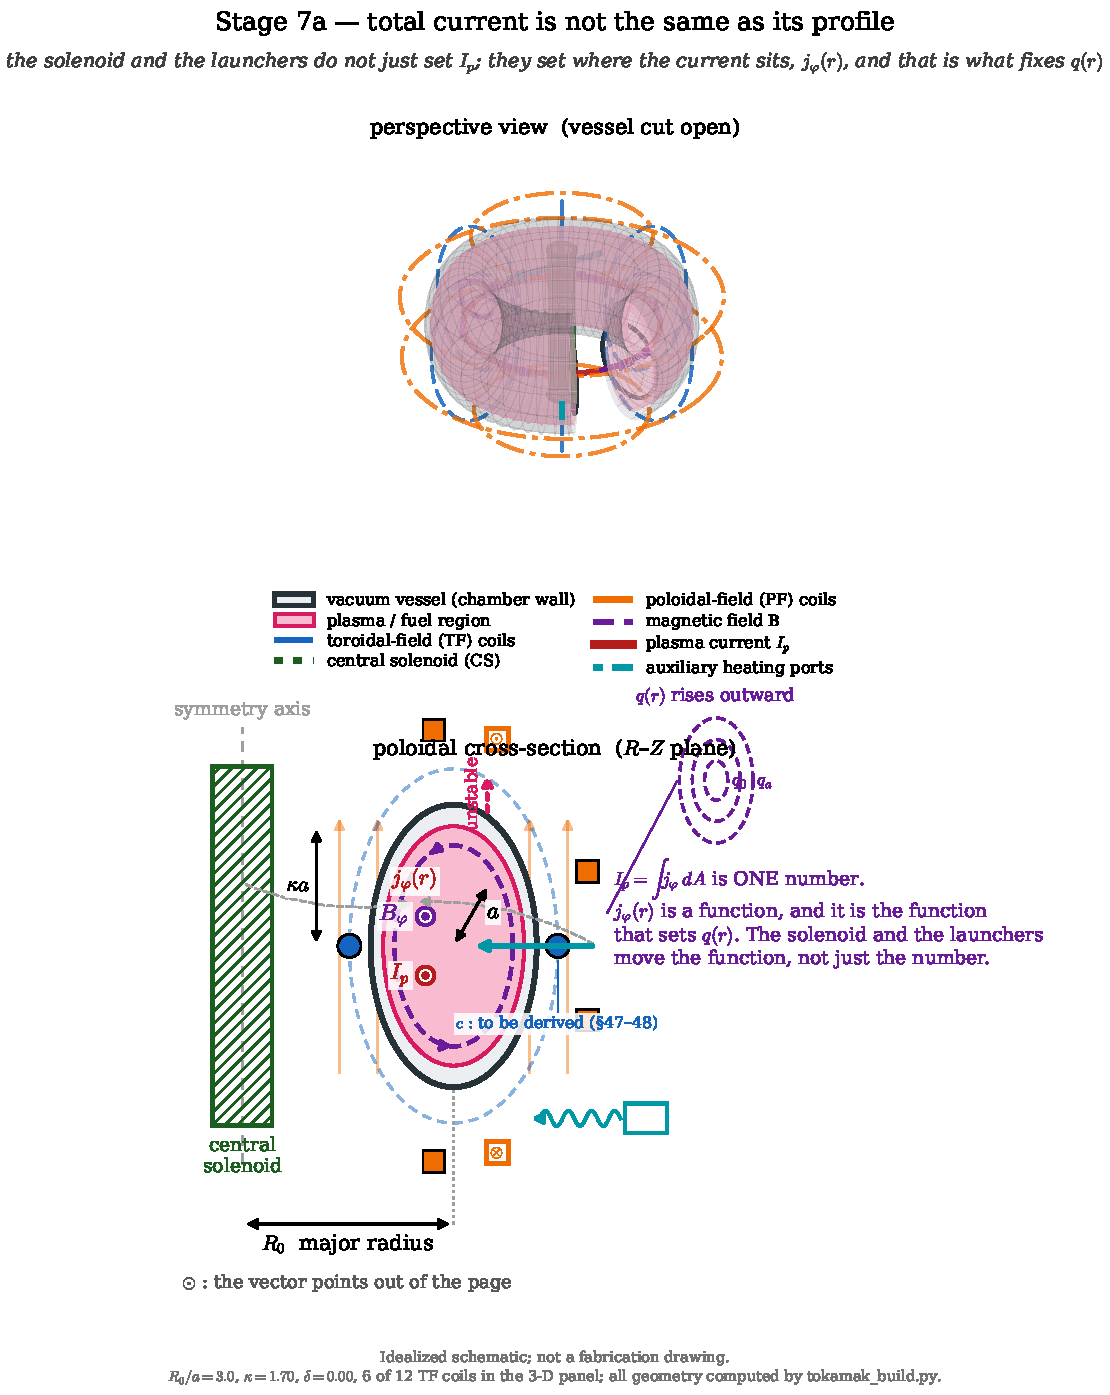
\includegraphics[width=1.0\textwidth]{figures/final/figM7a_profile_tall.pdf}
  \caption{Machine state: the current profile. Total current and its distribution $j_\varphi(r)$ are different quantities, and it is the profile that fixes $q(r)$. No new hardware appears --- this is an annotation layer.}
  \label{fig:figM7a_profile_tall}
\end{figure}


\designconsequence{The next design calculations must carry both a global current $I_p$
and a profile $q(r)$. That added bookkeeping is not mathematical fussiness: it records
which field lines and which stability limits the plasma actually contains.}
% ============================= PAGE 17 ==============================
\newpage
\section*{17. Why field strength and volume dominate the first performance estimate}

A fusion reaction needs one deuterium ion and one tritium ion. In a roughly equal D--T
mixture, the number of reaction opportunities per unit volume is proportional to $n^2$,
where $n$ is a representative fuel density. At a fixed useful temperature, the
reactivity $\langle\sigma v\rangle$ is also fixed, so
\begin{equation}
 P_{\rm fus}\propto n^2 V.
 \label{eq:pfus-density}
\end{equation}
This is a scaling statement, not yet a reactor-power calculation: the missing
proportionality constant contains the reaction energy and $\langle\sigma v\rangle(T)$.

For a fully ionized, equal-temperature D--T plasma, ions and electrons both contribute
to pressure, so $p\simeq 2nT$. The beta definition from page 8 gives
$p=\beta B_0^2/(2\mu_0)$ in this reduced scaling model. Therefore, at fixed $T$,
\begin{equation}
 n\propto\beta B_0^2,\qquad
 P_{\rm fus}\propto\beta^2B_0^4 V
 \propto\beta^2B_0^4R_0a^2\kappa.
 \label{eq:pfus-scaling}
\end{equation}
The fourth power of field is the memorable point. If all the stated assumptions hold,
raising $B_0$ slightly has a much larger effect on this estimate than raising it by the
same percentage appears to have at first glance. That is a motivation, not permission,
to choose an arbitrarily large field: coils, stresses, superconductors, plasma limits,
and the central stack will later impose the corresponding prices.

\friedbergvariable{$B_0$ and $\beta$}{Equation~\eqref{eq:pfus-scaling}
is the first bridge from plasma equilibrium to reactor output. It explains why the
toroidal field $B_0$, normalized pressure $\beta$, and shaped volume
$2\pi^2R_0a^2\kappa$ recur throughout Friedberg's design closure. The equation is a
conditional scaling law; temperature, confinement, and stability have not been
eliminated.}

\model{This page holds $T$, fuel mix, and $\langle\sigma v\rangle$ fixed, identifies
the confining field with $B_0$, and ignores profile factors. The actual D--T reactivity
varies strongly with temperature. The purpose is to derive the dependence that remains
once a target operating temperature has been chosen, not to replace a reactivity model.}

\imagebrief{Cumulative construction state 7: performance quantities attached to the
partly revealed machine}{Use the stage-6 conventional tokamak. Add unobtrusive labels
for $R_0$, $a$, $\kappa$, $B_0$, and $I_p$ on the actual machine components, plus a
small side panel showing the derived chain
$P_{\rm fus}\propto n^2V\propto\beta^2B_0^4R_0a^2\kappa$.
The figure must retain all previously introduced components and make clear that this is
a scaling law, not a claim of net electrical power.}

\begin{figure}[htbp]\centering
  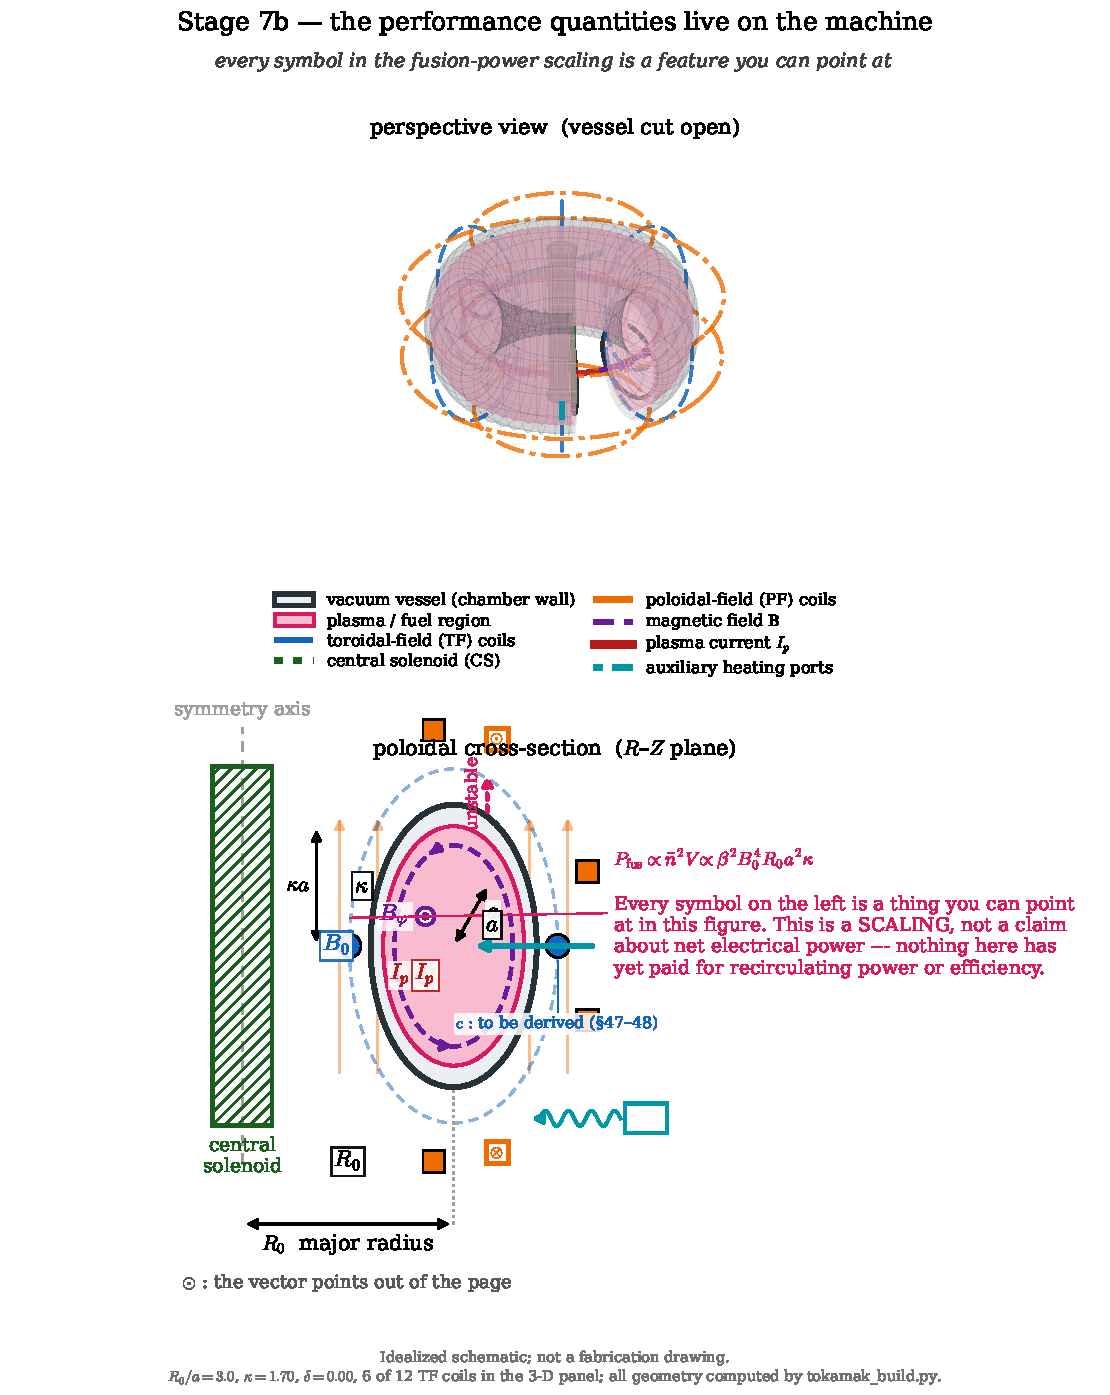
\includegraphics[width=1.0\textwidth]{figures/final/figM7b_performance_tall.pdf}
  \caption{Machine state: the performance quantities, attached to the machine. Every symbol in the fusion-power scaling is a feature that can be pointed at.}
  \label{fig:figM7b_performance_tall}
\end{figure}


\designconsequence{The machine now has a reason to seek strong field, high allowed
pressure, and useful volume. The remainder of the thesis must show whether these desires
can coexist with current limits, confinement, materials, coil technology, and power
balance.}

% ============================= PAGE 18 ==============================
\newpage
\section*{18. A ledger before optimization: what has actually been derived?}

These pages have built a ledger of demands rather than selected a tokamak by
declaration. It prevents improving one formula while silently violating another.

\begin{center}
\renewcommand{\arraystretch}{1.12}
\begin{tabular}{p{0.23\textwidth}p{0.31\textwidth}p{0.34\textwidth}}
\textbf{Quantity} & \textbf{What it measures} & \textbf{Why it cannot be chosen alone}\\
\hline
$R_0,\ a,\ A=R_0/a$ & Overall and cross-sectional size & Set geometry, volume, and aspect ratio.\\
$B_0$ & Toroidal confining field & Shrinks gyro-orbits; appears as $B_0^4$ in the conditional power scaling.\\
$I_p$ & Toroidal plasma current & Creates poloidal field, but is bounded by the safety-factor constraint.\\
$q(r),\ q_*$ & Field-line pitch and its shaped global measure & Depend on current distribution as well as total current.\\
$\kappa$ & Vertical elongation & Increases volume and the reduced $I_p$ allowance; requires shaping and feedback.\\
$n,\ T,\ p,\ \beta$ & Fuel state and magnetic-pressure fraction & Set reaction opportunity and challenge confinement and stability.\\
$\tau_E$ & Energy-confinement time & Decides whether heating can outrun losses; it remains to be derived and modeled.\\
\end{tabular}
\end{center}

The drawing now has earned components: vacuum and magnetic field for hot fuel; a torus
to remove open ends; a solenoid and plasma current for the poloidal field; PF coils for
position and shape; feedback for vertical stability; and heating/current-drive ports
because the transformer has a finite clock.

\imagebrief{Construction-atlas checkpoint}{Make a one-page cumulative annotated
cross-section and toroidal cutaway of the conventional tokamak derived so far: vacuum
vessel; plasma; TF coils and $B_\varphi$; central solenoid and induced $I_p$; PF/shaping
coils; elongated boundary with $a$, $\kappa a$, and $R_0$; magnetic sensors and feedback;
heating/current-drive port. Number each component by the page where its physical need
was derived. Leave out divertor, blanket, shielding, superconducting magnets, and all
spherical-tokamak geometry: those have not yet earned their place.}

\begin{figure}[htbp]\centering
  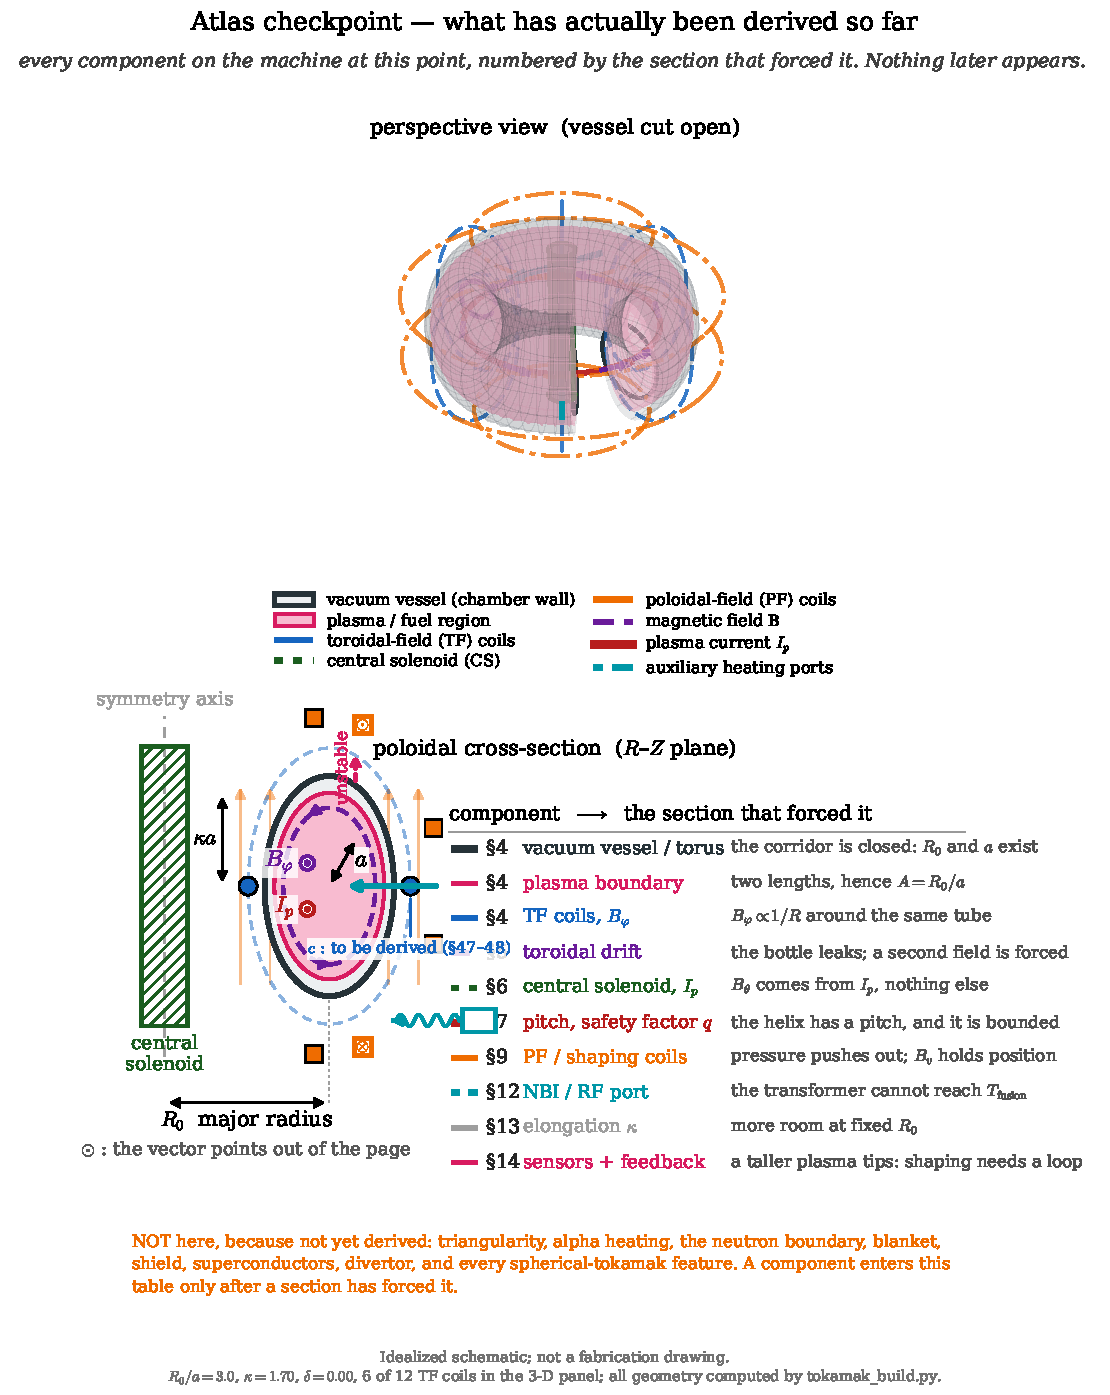
\includegraphics[width=1.0\textwidth]{figures/final/figM7c_atlas1_tall.pdf}
  \caption{Atlas checkpoint. Every component derived so far, numbered by the section that forced it. Nothing later than \S18 appears: a part enters this table only after a section has made it necessary.}
  \label{fig:figM7c_atlas1_tall}
\end{figure}


\supportingquantity{first coupled ledger}{The variables in this ledger are the
minimum state carried forward into the Friedberg-style closure problem. A proposed
parameter set is acceptable only when the equations that constrain \emph{all} of them
are checked together.}

\designconsequence{The ordinary tokamak is now visible, but only as the accumulated
answer to specific physical failures. The next section can add the remaining reactor
subsystems in the same discipline: name the failure, derive the demand, then add the
component and its variables to the ledger.}

% ============================= PAGE 19 ==============================
\newpage
\section*{19. The next shape parameter: a D rather than an ellipse}

Elongation says how tall the cross-section is. It does not say whether its upper point
lies above the geometric centreline or leans toward the central hole. To name that
second feature without drawing a machine first, take the boundary
\begin{equation}
 R(\theta)=R_0+a\cos(\theta+x\sin\theta),\qquad
 Z(\theta)=\kappa a\sin\theta,\qquad x=\arcsin\delta .
 \label{eq:miller-boundary}
\end{equation}
This is a useful \emph{coordinate chart} for a family of closed curves, not a law of
nature. At the top, $\theta=\pi/2$, Eq.~\eqref{eq:miller-boundary} gives
\[
 R_{\rm top}=R_0+a\cos(\pi/2+x)=R_0-a\sin x=R_0-\delta a.
\]
Thus
\begin{equation}
 \delta=\frac{R_0-R_{\rm top}}{a}
 \label{eq:triangularity}
\end{equation}
is the normalized inward displacement of the top point. Positive $\delta$ makes the
familiar D-like cross-section; $\delta=0$ returns the ellipse of page 13.

For small $\delta$, we can see exactly which new geometric pattern it adds. Use
$\cos(\theta+x\sin\theta)=\cos\theta-x\sin^2\theta+O(x^2)$ and
$\sin^2\theta=(1-\cos2\theta)/2$. Since $x=\delta+O(\delta^3)$,
\begin{equation}
 R(\theta)=R_0-\frac{a\delta}{2}+a\cos\theta+
            \frac{a\delta}{2}\cos2\theta+O(\delta^2).
 \label{eq:triangular-harmonic}
\end{equation}
The first cosine describes the ordinary left-right radius. Triangularity is, to
leading order, a second angular harmonic plus a small centering shift. That is why it
needs more than the simple shaping action which made the ellipse.

\supportingquantity{$\delta$ (triangularity)}{Equation~\eqref{eq:triangularity}
defines the D-shape parameter carried in reactor equilibria. Equation~\eqref{eq:triangular-harmonic}
shows that it is an independently adjustable geometric feature, not another name for
elongation. Its stability benefit, when present, must be established separately from
this definition.}

\imagebrief{Cumulative construction state 8: add triangularity}{Start with the elongated,
feedback-controlled conventional tokamak. Replace the ellipse in the cross-sectional
inset with two labelled boundaries, $\delta=0$ and $\delta>0$, keeping the same $a$,
$\kappa a$, PF coils, and central solenoid. Mark the inward shift $\delta a$ of the
top point. The image must make clear that triangularity changes plasma shape, not the
shape of the toroidal-field coils.}

\begin{figure}[htbp]\centering
  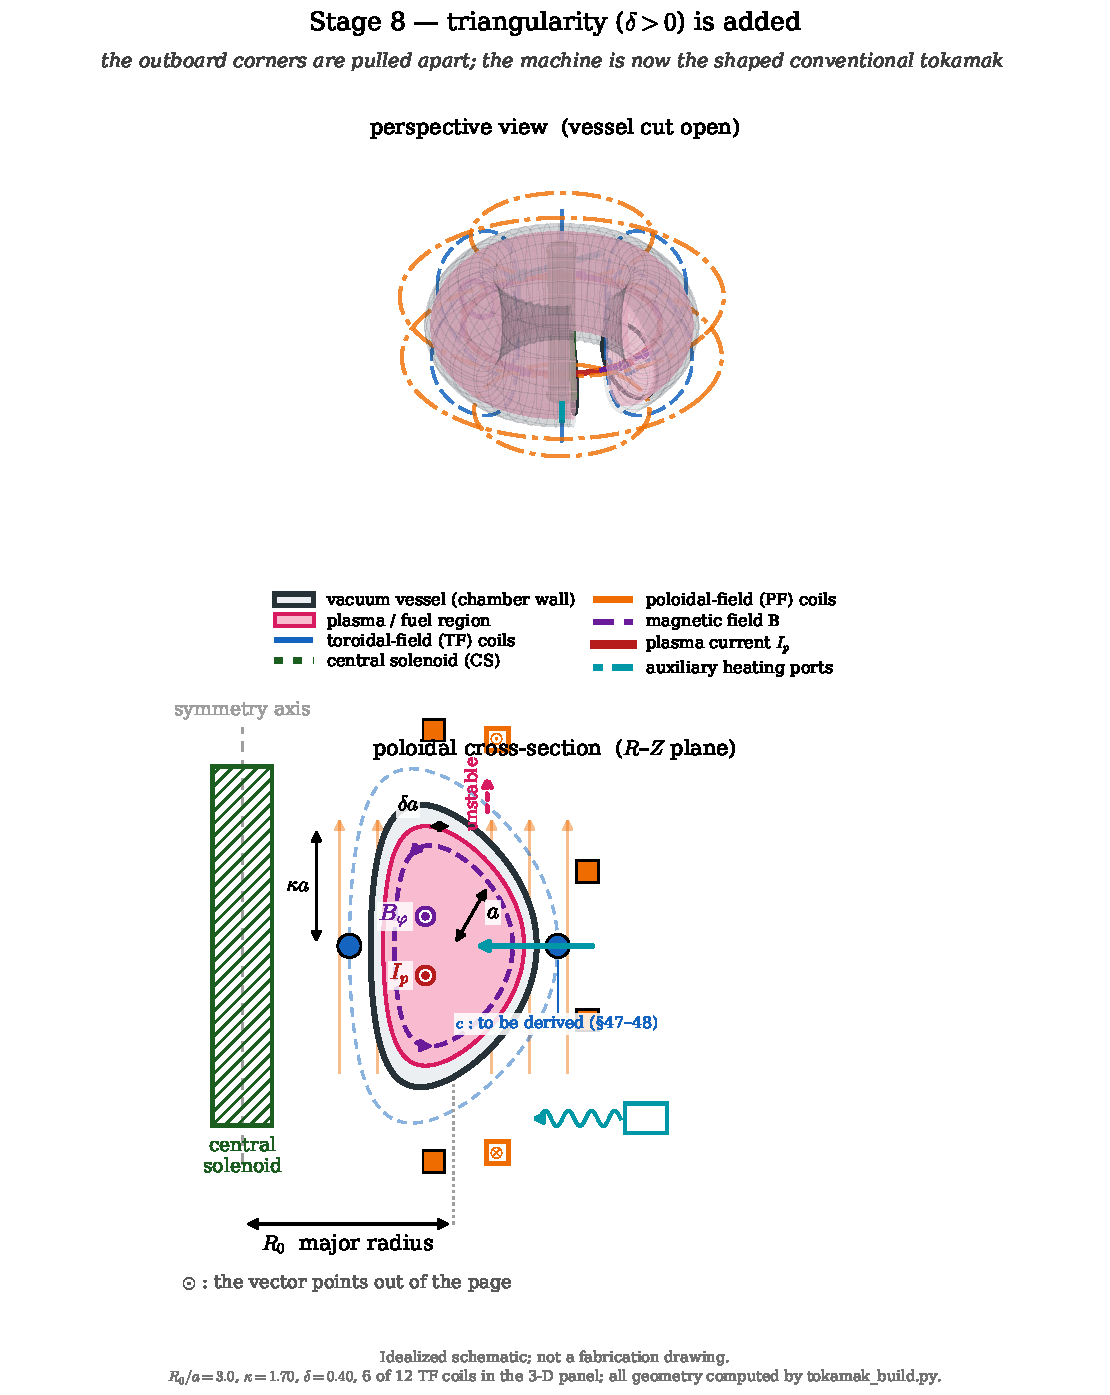
\includegraphics[width=1.0\textwidth]{figures/final/figM8_stage8_tall.pdf}
  \caption{Machine state: triangularity. A D rather than an ellipse. No new species of coil appears --- consistent with the text, the existing PF set has simply gained another job.}
  \label{fig:figM8_stage8_tall}
\end{figure}


\model{Equation~\eqref{eq:miller-boundary} is the Miller local-equilibrium shape
parameterization. Its role here is definitional and geometric; it is not derived from
Maxwell's equations. A freely available analytic-equilibrium treatment by Cerfon and
Freidberg is cited on page 10.}

\designconsequence{A D-shaped boundary creates a new demand on the PF system: it must
produce another independently controllable field pattern. The machine has not gained a
new species of coil, but the coil set has gained another job.}
% ============================= PAGE 20 ==============================
\newpage
\section*{20. Why more shape means more carefully placed PF coils}

Outside the plasma there is no plasma current density. In that region, magnetic field
lines from PF coils satisfy the source-free magnetostatic equations
\[
 \nabla\times\mathbf B=0,\qquad \nabla\cdot\mathbf B=0.
\]
The first equation permits a scalar magnetic potential, $\mathbf B=-\nabla\Phi$;
inserting it into the second gives $\nabla^2\Phi=0$. This is Laplace's equation.
Near the plasma centre, its smooth solutions can be organized by angular pattern.

The first three patterns have an immediate physical reading. A nearly uniform vertical
field translates the plasma radially. A field whose horizontal component grows with
height and whose vertical component grows with radius is a quadrupole: it stretches or
squeezes the boundary into an ellipse. The next pattern, a hexapole, has the angular
structure needed for the leading $\cos2\theta$ term in Eq.~\eqref{eq:triangular-harmonic}.
These are not three unrelated inventions. They are the first terms in one local
expansion of the externally applied field.

A simple two-dimensional example makes the hierarchy visible. The harmonic functions
\[
 \Phi_1=C_1r\sin\theta,\qquad
 \Phi_2=C_2r^2\sin2\theta,\qquad
 \Phi_3=C_3r^3\sin3\theta
\]
all solve $\nabla^2\Phi=0$ in polar coordinates. Taking $-\nabla\Phi$ turns their
successive angular structures into the uniform, quadrupole, and hexapole-like field
patterns just described. A coil system chooses the coefficients $C_1,C_2,C_3$ by its
locations and currents. The exact tokamak geometry is toroidal rather than this flat
example, but the local lesson survives: more detailed boundary shape requires more
independent field moments.

\imagebrief{Physics sketch: the external-field harmonic ladder}{Make a separate
three-panel line drawing, not a cumulative machine view. Panel 1: uniform vertical
field translating a circular plasma. Panel 2: quadrupole field stretching it into an
ellipse. Panel 3: hexapole-like shaping field producing a D-like boundary. Label the
patterns $C_1,C_2,C_3$ and state that real PF-coil geometry is toroidal. Generate from
a reproducible script.}

\begin{figure}[htbp]\centering
  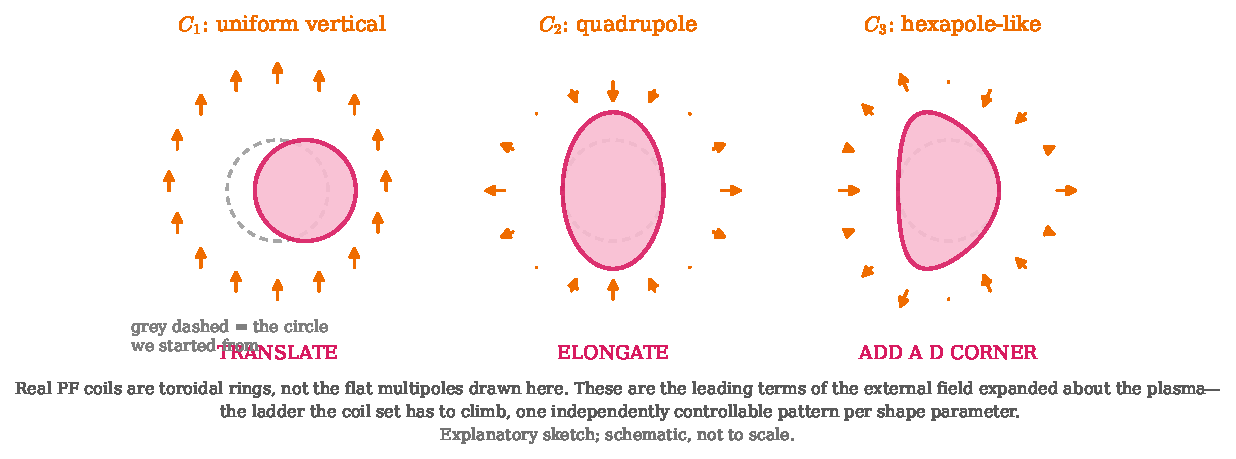
\includegraphics[width=1.0\textwidth]{figures/final/figS_harmonic_ladder.pdf}
  \caption{Physics sketch: the external-field harmonic ladder. \schematicnote}
  \label{fig:figS_harmonic_ladder}
\end{figure}


\designconsequence{The phrase shape control hides a finite-dimensional control
problem. A reactor needs enough independently powered PF circuits, appropriately
located, to control position, elongation, and triangularity while the plasma current
and pressure change.}

% ============================= PAGE 21 ==============================
\newpage
\section*{21. The plasma as a fluid: the equilibrium equation}

The single-particle Lorentz force was enough to explain gyro-orbits and field-guided
motion. To decide the shape of a plasma containing an enormous number of particles, we
add their forces per unit volume. Let $\rho_m$ be mass density, $\mathbf u$ the bulk
velocity, $p$ the scalar pressure, and $\mathbf j$ the current density. Momentum
conservation for a small fluid element is
\begin{equation}
 \rho_m\frac{d\mathbf u}{dt}=\mathbf j\times\mathbf B-\nabla p.
 \label{eq:mhd-momentum}
\end{equation}
The magnetic term is simply the Lorentz force $q\mathbf v\times\mathbf B$ summed
over charged particles per unit volume. The pressure term points from high pressure
toward low pressure: a small box has slightly greater inward force on its high-pressure
face than on its low-pressure face.

For the slowly changing equilibrium that defines the intended plasma boundary, set the
bulk acceleration to zero. Equation~\eqref{eq:mhd-momentum} becomes
\begin{equation}
 \boxed{\nabla p=\mathbf j\times\mathbf B.}
 \label{eq:force-balance-local}
\end{equation}
This one equation has an exceptionally concrete reading. At every location, magnetic
force density must exactly push back against the local pressure gradient. If it does
not, the plasma moves; the supposed boundary is not an equilibrium.

Dot Eq.~\eqref{eq:force-balance-local} with $\mathbf B$. Since
$\mathbf B\cdot(\mathbf j\times\mathbf B)=0$, we obtain
\[
 \mathbf B\cdot\nabla p=0.
\]
Pressure is therefore constant along each magnetic field line in this equilibrium
model. When field lines densely cover a nested magnetic surface, pressure is constant
on that surface too. This is the precise reason flux surfaces became more than a
drawing convention on page 10: they are also surfaces of constant pressure.

\supportingquantity{$p(\psi)$}{In an axisymmetric equilibrium, pressure becomes a
function of the flux-surface label $\psi$. This is one of the inputs to the
Grad--Shafranov equation and later controls $\beta$, fusion power density, and
pressure-driven stability.}

\model{Equation~\eqref{eq:mhd-momentum} assumes a single fluid with isotropic
pressure and neglects viscosity, kinetic orbit effects, and rapid flows. Those effects
matter in detailed equilibrium reconstruction; this model is the minimum one needed to
derive the ordinary tokamak equilibrium equation.}

\designconsequence{A plasma boundary is not a material container. It is a
self-consistent solution of pressure, plasma current, and externally produced field.
The next pages derive the equation that tests that consistency.}

% ============================= PAGE 22 ==============================
\newpage
\section*{22. A flux function compresses the axisymmetric geometry}

Use cylindrical coordinates $(R,\varphi,Z)$ and assume axisymmetry:
$\partial/\partial\varphi=0$. The toroidal component of the magnetic field is written
as $B_\varphi=F(R,Z)/R$. For the poloidal part, define a scalar $\psi(R,Z)$ by
\begin{equation}
 \mathbf B_p=\frac{1}{R}\nabla\psi\times\hat{\boldsymbol\varphi}.
 \label{eq:flux-representation}
\end{equation}
Writing out the cross product gives
\[
 B_R=-\frac1R\frac{\partial\psi}{\partial Z},\qquad
 B_Z=\frac1R\frac{\partial\psi}{\partial R}.
\]
Substitution into
$\nabla\cdot\mathbf B_p=R^{-1}\partial_R(RB_R)+\partial_ZB_Z$
shows the two mixed derivatives cancel. Thus Eq.~\eqref{eq:flux-representation}
automatically satisfies $\nabla\cdot\mathbf B_p=0$.

A curve of constant $\psi$ has tangent displacement $d\boldsymbol\ell$ satisfying
$\nabla\psi\cdot d\boldsymbol\ell=0$. Equation~\eqref{eq:flux-representation}
also gives $\mathbf B_p\cdot\nabla\psi=0$. Hence the poloidal field is tangent to
the curves $\psi=\text{constant}$; rotating such a curve around the symmetry axis
creates one magnetic surface. The symbol $\psi$ is therefore a surface label. Up
to a conventional factor of $2\pi$, it is also the poloidal magnetic flux enclosed
by that surface.

Putting the pieces together,
\begin{equation}
 \mathbf B=\frac{1}{R}\nabla\psi\times\hat{\boldsymbol\varphi}
            +\frac{F}{R}\hat{\boldsymbol\varphi}.
 \label{eq:axisymmetric-B}
\end{equation}
This is not an approximation. It is a representation of any sufficiently smooth,
axisymmetric, divergence-free magnetic field away from the coordinate axis.

\imagebrief{Physics sketch: reading $\psi$}{Draw an axisymmetric poloidal cross-section
with nested curves labelled $\psi_1,\psi_2,\psi_3$, arrows tangent to the curves for
$\mathbf B_p$, and a curled toroidal arrow for $B_\varphi$. Include a small arrow
for $\nabla\psi$ perpendicular to the surfaces. Do not show hardware; this is the
mathematical map that makes flux surfaces intelligible.}

\begin{figure}[htbp]\centering
  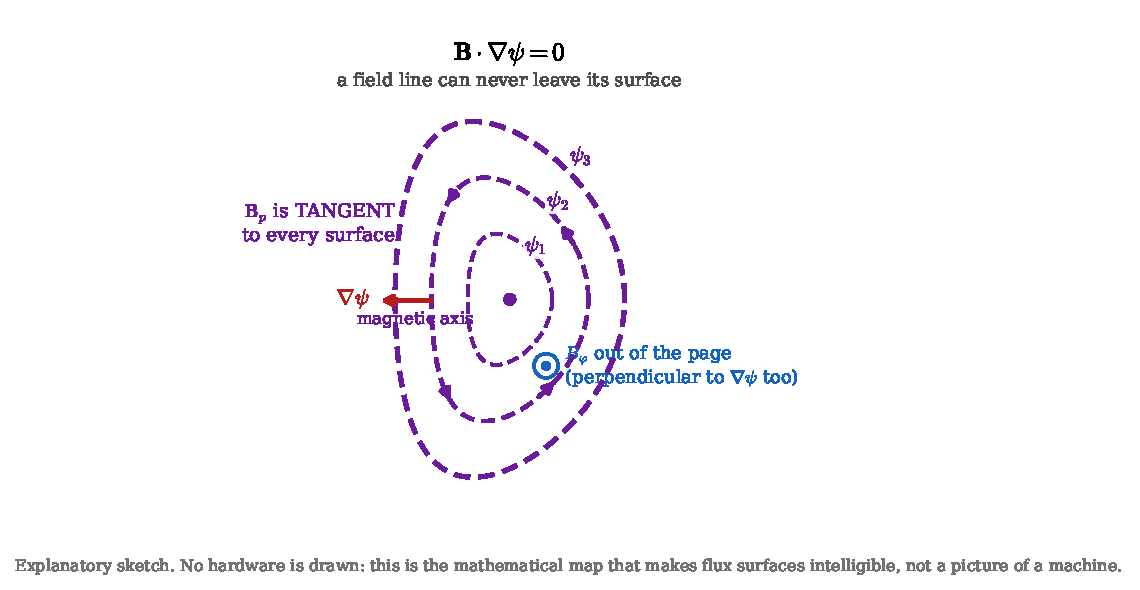
\includegraphics[width=1.0\textwidth]{figures/final/figS_reading_psi.pdf}
  \caption{Physics sketch: reading $\psi$. \schematicnote}
  \label{fig:figS_reading_psi}
\end{figure}


\designconsequence{The entire two-dimensional equilibrium can now be described by
two scalar functions, $\psi(R,Z)$ and $F(R,Z)$. This is the compression that makes
a calculable plasma boundary possible.}

% ============================= PAGE 23 ==============================
\newpage
\section*{23. Deriving the Grad--Shafranov equation, one force at a time}

Ampere's law without displacement current is
$\mu_0\mathbf j=\nabla\times\mathbf B$. Insert Eq.~\eqref{eq:axisymmetric-B}.
The toroidal component comes only from the curl of $\mathbf B_p$:
\begin{equation}
 j_\varphi=-\frac{1}{\mu_0R}\Delta^*\psi,\qquad
 \Delta^*\psi\equiv R\frac{\partial}{\partial R}
 \left(\frac1R\frac{\partial\psi}{\partial R}\right)
 +\frac{\partial^2\psi}{\partial Z^2}.
 \label{eq:gradstar}
\end{equation}
This follows directly by differentiating $B_R$ and $B_Z$ written on page 22:
$(\nabla\times\mathbf B_p)_\varphi=\partial_ZB_R-\partial_RB_Z$.

The toroidal component of the equilibrium force in Eq.~\eqref{eq:force-balance-local}
must vanish because $p$ is axisymmetric. It gives
$\mathbf B_p\cdot\nabla F=0$, so $F$ is constant along the poloidal field and may
be written $F=F(\psi)$. The same argument on page 21 gave $p=p(\psi)$. With those
two results, direct cross products reduce the force balance to a single direction,
normal to the surfaces:
\[
 \mathbf j\times\mathbf B=
 -\frac{1}{\mu_0R^2}\left(\Delta^*\psi+F\frac{dF}{d\psi}\right)\nabla\psi,
 \qquad
 \nabla p=\frac{dp}{d\psi}\nabla\psi .
\]
The common vector $\nabla\psi$ can be cancelled wherever it is nonzero. The result is
\begin{equation}
 \boxed{\Delta^*\psi=-\mu_0R^2\frac{dp}{d\psi}
                    -F\frac{dF}{d\psi}.}
 \label{eq:grad-shafranov}
\end{equation}
This is the Grad--Shafranov equation. It has no hidden tokamak magic: the first term
is the pressure-gradient demand and the second represents toroidal-field/current
effects. A boundary shape and the two functions $p(\psi)$ and $F(\psi)$ determine
the equilibrium problem; external coils supply the boundary conditions.

\supportingquantity{$\psi$, $p(\psi)$, and $F(\psi)$}{These are the minimal
axisymmetric-equilibrium data beneath the reactor variables. They determine whether a
proposed $I_p$, shape, and pressure can share nested magnetic surfaces.}

\model{The cancellation leading to Eq.~\eqref{eq:grad-shafranov} fails at magnetic
nulls such as an X-point, where $\nabla\psi=0$; the equation itself remains the
standard equilibrium equation but the local geometric argument must be treated with
care there.}

% ============================= PAGE 24 ==============================
\newpage
\section*{24. What the equilibrium equation says before it is solved}

Equation~\eqref{eq:grad-shafranov} is a differential equation, not a ready-made
shape. To solve it, one specifies a vacuum-vessel or plasma-boundary condition for
$\psi$, the external-coil currents that contribute to that condition, and profiles
for $p(\psi)$ and $F(\psi)$. The solution then reports the nested surfaces, the
plasma current, and the position of the magnetic axis. This is why a tokamak needs
both a physics model and a coil-control model.

The equation also explains an effect visible in real cross-sections: the magnetic
axis usually shifts outward from the geometric centre. Pressure gradients and the
plasma's own poloidal field produce an outward hoop tendency; the poloidal-field
system counters it. The shift is called the Shafranov shift. Its exact size depends
on the profiles, so it must not be inserted as a universal number. The robust
conclusion is only the causal one: increasing pressure or current changes the
equilibrium shape, and fixed coil currents will no longer hold the intended boundary.

This is also the cleanest place to separate two kinds of D. A D-shaped \emph{plasma}
boundary is selected through $\delta$ and the equilibrium/stability tradeoffs. A
D-shaped \emph{toroidal-field coil}, when used, is a mechanical solution for reducing
bending stress in a conductor exposed to a field that varies approximately as $1/R$.
They can appear in the same machine, but they solve different equations and neither
should be used to explain the other.

\imagebrief{Cumulative construction state 9: equilibrium is a moving target}{Use the
stage-8 conventional tokamak cross-section with shaped PF coils. Draw two nested
sets of flux surfaces: a low-pressure reference centered near the geometric axis and
a higher-pressure/current case shifted slightly outward. Label $\psi$, $p(\psi)$,
and the PF-coil currents. Show the same hardware in both cases; the message is that
operating state changes the demanded coil settings.}

\begin{figure}[htbp]\centering
  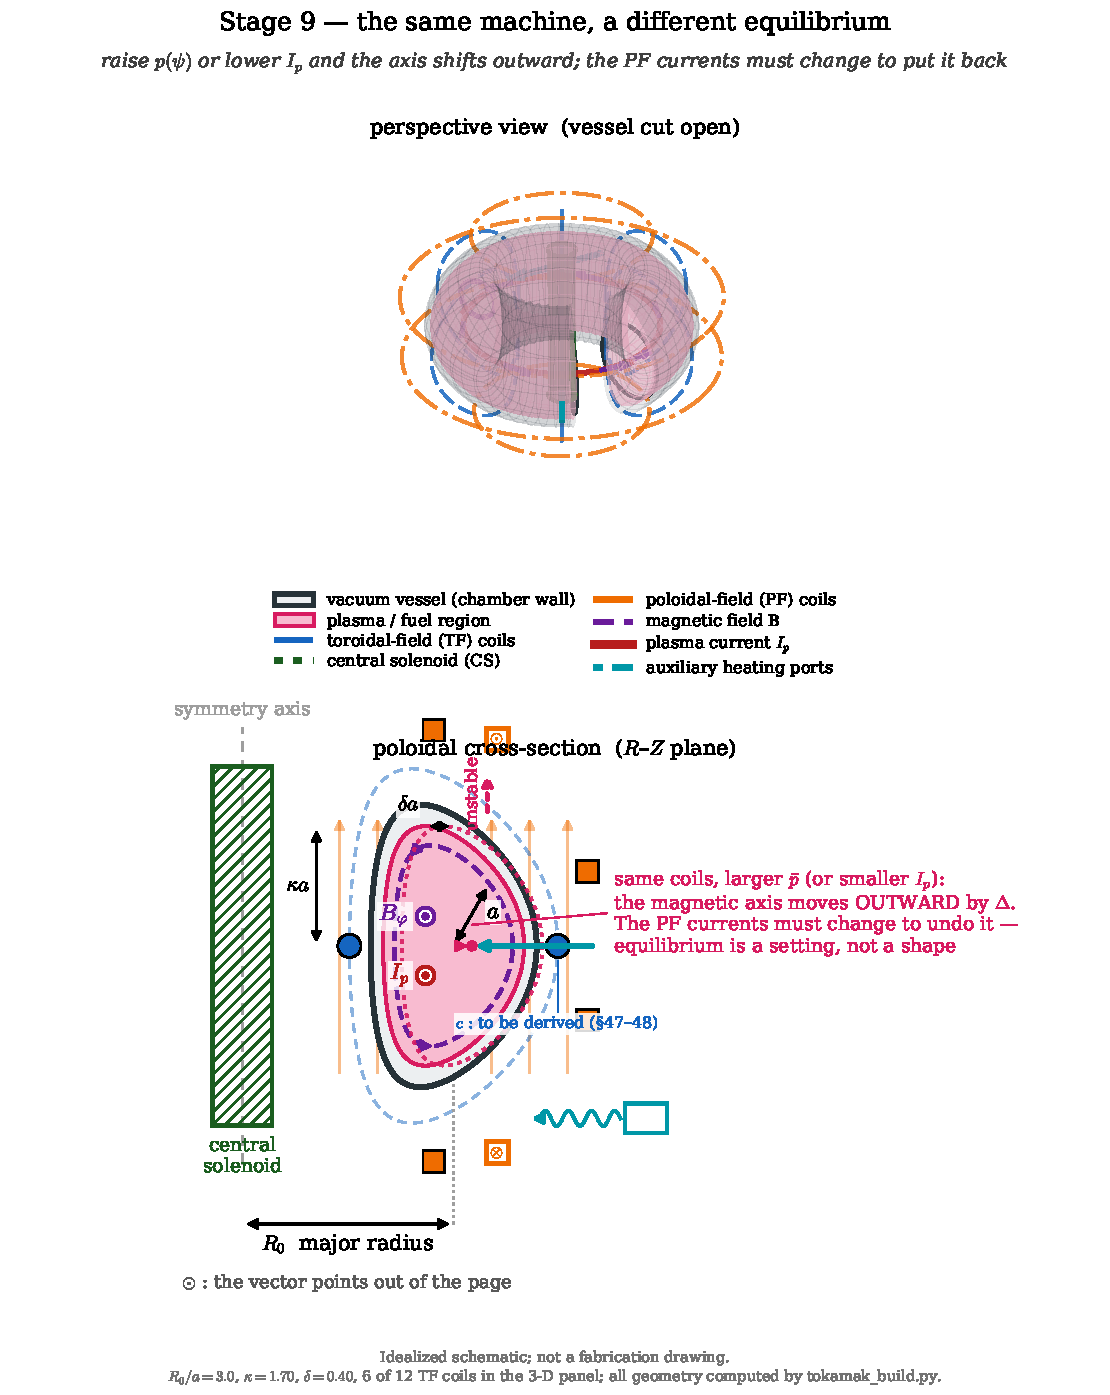
\includegraphics[width=1.0\textwidth]{figures/final/figM9_stage9_tall.pdf}
  \caption{Machine state: the same machine, a different equilibrium. Raise $\bar p$ or lower $I_p$ and the magnetic axis shifts outward; the PF currents must change to undo it. The shift drawn is illustrative --- its size follows from Grad--Shafranov.}
  \label{fig:figM9_stage9_tall}
\end{figure}


\designconsequence{The physical boundary cannot be designed once and forgotten.
Every planned operating point requires an equilibrium and a control solution. This is
why later performance calculations must report profiles and margins, not merely a list
of nominal dimensions.}
% ============================= PAGE 25 ==============================
\newpage
\section*{25. From individual collisions to a fusion-power density}

Consider a small volume $dV$ containing $n_DdV$ deuterons and $n_TdV$ tritons.
Choose one deuteron. During a short time $dt$, tritons with relative speed $v$
sweep through the effective collision tube of area $\sigma(v)$ and length $vdt$.
The expected number of its reactions is
\[
 n_T\,\sigma(v)\,v\,dt.
\]
Particles in a thermal plasma do not all have the same relative speed. Average this
expression over the normalized relative-speed distribution and multiply by the
number $n_DdV$ of deuterons. Dividing by $dVdt$ gives the reaction rate per unit
volume:
\begin{equation}
 {\cal R}_{DT}=n_Dn_T\langle\sigma v\rangle,\qquad
 \langle\sigma v\rangle=\int_0^\infty \sigma(v)v\,f_{\rm rel}(v)\,dv .
 \label{eq:reaction-rate}
\end{equation}
The brackets are an average, not a new force law. All difficult nuclear physics is
contained in the measured cross section $\sigma(v)$; all thermal statistics is
contained in $f_{\rm rel}(v)$.

If each reaction releases total energy $E_f=17.6\,\mathrm{MeV}$, then
\begin{equation}
 p_{\rm fus}=E_f{\cal R}_{DT}
 =E_f n_Dn_T\langle\sigma v\rangle,\qquad
 P_{\rm fus}=p_{\rm fus}V.
 \label{eq:pfus-exact}
\end{equation}
This is the exact starting point behind the proportional sign on page 17. It says
why a fusion plant cannot be discussed using temperature alone: density, volume, and
the sharply temperature-dependent reactivity all matter.

\supportingquantity{$\langle\sigma v\rangle(T)$}{The D--T reactivity turns a chosen
temperature into a fusion-rate coefficient in Eq.~\eqref{eq:reaction-rate}. It is
a measured nuclear input, not a free reactor-design variable and not something this
thesis should replace with an unsupported universal formula.}

\model{Equation~\eqref{eq:reaction-rate} assumes independent binary collisions and
a thermal distribution. At reactor density, D--T fusion remains dilute enough for that
description; collective plasma physics controls confinement, not the short-range
nuclear reaction once two ions meet.}

\designconsequence{Fusion output grows with a product of densities. The next question
is therefore a design question: for a fixed amount of fuel, which mixture makes that
product largest?}

% ============================= PAGE 26 ==============================
\newpage
\section*{26. Why the fuel mixture is nearly fifty--fifty}

Let the total fuel-ion density be fixed:
\[
 n_i=n_D+n_T.
\]
Write $n_D=xn_i$. Then $n_T=(1-x)n_i$, and the density product in
Eq.~\eqref{eq:pfus-exact} is
\begin{equation}
 n_Dn_T=x(1-x)n_i^2.
 \label{eq:mixture-product}
\end{equation}
Complete the square:
\[
 x(1-x)=x-x^2=\frac14-\left(x-\frac12\right)^2.
\]
The squared term is nonnegative, so the largest possible value is $1/4$, achieved
at $x=1/2$. Thus
\begin{equation}
 n_D=n_T=\frac{n_i}{2}
 \quad\Longrightarrow\quad
 p_{\rm fus}=\frac14n_i^2\langle\sigma v\rangle E_f.
 \label{eq:pfus-5050}
\end{equation}
This is an unusually clean design conclusion: equal fuel fractions maximize fusion
opportunities at fixed total ion density and temperature.

The pressure used in magnetic confinement also includes electrons. A quasi-neutral
50--50 D--T mixture has electron density $n_e=n_i$. If the ions and electrons share
a temperature $T$ measured in energy units, their ideal-gas pressures add:
\begin{equation}
 p=(n_i+n_e)T=2n_iT.
 \label{eq:plasma-pressure}
\end{equation}
Combining Eqs.~\eqref{eq:pfus-5050} and \eqref{eq:plasma-pressure} explains the
scaling chain on page 17, but with its factors visible: at fixed $T$,
$n_i=p/(2T)$ and hence $p_{\rm fus}\propto p^2$.

\friedbergvariable{$T$, $n$, and $p$}{For the equal 50--50 mixture used here,
$n_i$ is the primary fuel-density variable $n$, and $p=2nT$. A claimed gain in
density at fixed magnetic field must therefore be checked against the pressure and
density limits separately.}

\imagebrief{Physics sketch: counting fusion pairs}{Make a small conceptual graphic
with two boxes containing the same total number of fuel ions: one unequal D--T mixture,
one equal mixture. Show the pair count proportional to $n_Dn_T$ and the completed-square
maximum at $n_D=n_T$. This is a reset explanatory sketch, not a machine drawing.}

\begin{figure}[htbp]\centering
  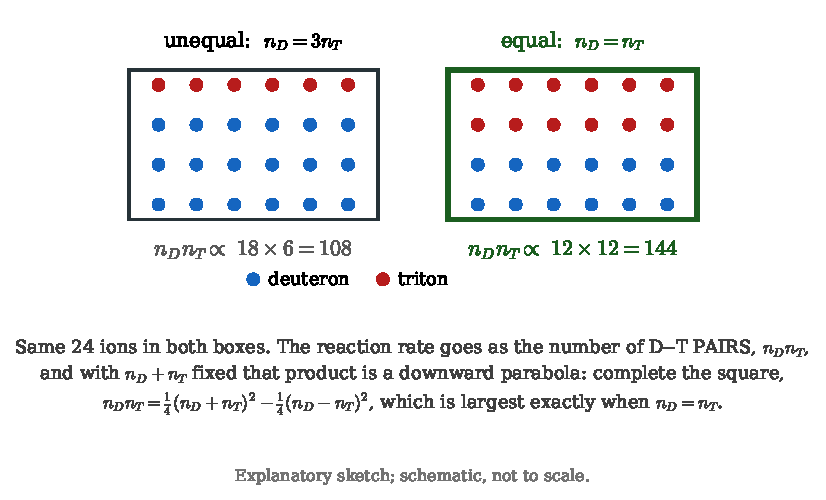
\includegraphics[width=1.0\textwidth]{figures/final/figS_fusion_pairs.pdf}
  \caption{Physics sketch: counting fusion pairs. \schematicnote}
  \label{fig:figS_fusion_pairs}
\end{figure}


\designconsequence{The density needed for power also creates pressure. The magnetic
field must therefore confine not only charged particles one at a time, but the
collective pressure of the mixture.}

% ============================= PAGE 27 ==============================
\newpage
\section*{27. Where the fusion energy goes decides what the machine must add}

The D--T products are an alpha particle and a neutron. In the center-of-mass frame
they leave with equal and opposite momentum, so their momentum magnitudes are equal:
$m_\alpha v_\alpha=m_nv_n$. Their kinetic energies are
$E_\alpha=p^2/(2m_\alpha)$ and $E_n=p^2/(2m_n)$. Therefore
\[
 \frac{E_n}{E_\alpha}=\frac{m_\alpha}{m_n}\simeq4,\qquad
 E_\alpha=\frac15E_f\simeq3.5\,\mathrm{MeV},\quad
 E_n=\frac45E_f\simeq14.1\,\mathrm{MeV}.
\]
The alpha is charged. It remains magnetically confined long enough to slow down by
collisions and can heat the plasma. The neutron has no electric charge, so magnetic
fields do not bend it; it escapes the plasma and deposits its energy only after
meeting material outside the vacuum region.

Define alpha heating by $P_\alpha=(E_\alpha/E_f)P_{\rm fus}$ before loss channels.
Similarly, $P_n=(E_n/E_f)P_{\rm fus}$ is neutron power. This is not a minor accounting
choice. A burning plasma needs the alpha fraction to replace energy
lost from the plasma. A power plant needs the neutron fraction to be captured in a
future blanket, which will earn its place later by this physical necessity.

\supportingquantity{$P_\alpha$ and $P_n$}{The split $P_\alpha=P_{\rm fus}/5$ and
$P_n=4P_{\rm fus}/5$ separates plasma self-heating from energy that leaves the
magnetic bottle. It is the bridge between the plasma power balance and the later
reactor-around-the-plasma discussion.}

\imagebrief{Cumulative construction state 10: alpha heating and neutron escape}{Use
the existing conventional tokamak cross-section, without adding a blanket. Inside the
plasma, show a short spiral alpha trajectory and label $3.5$ MeV self-heating. Draw
straight neutral-neutron arrows crossing the vacuum region and stopping at a clearly
labelled future boundary outside the current derived machine. State explicitly that
the blanket is not yet drawn because it has not yet been derived.}

\begin{figure}[htbp]\centering
  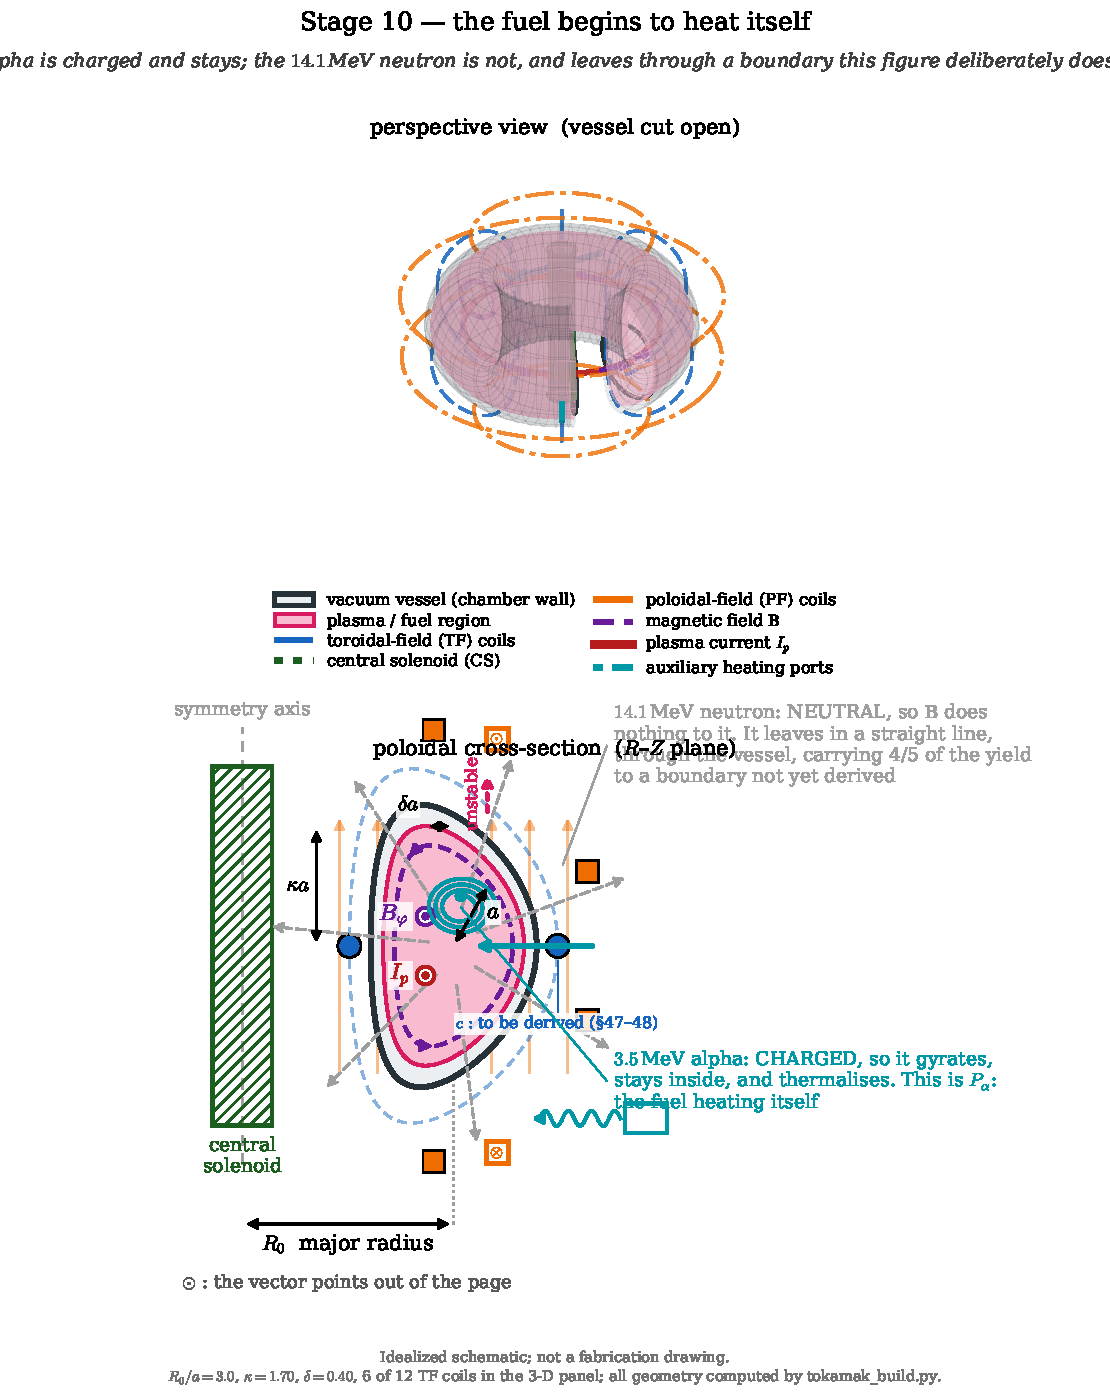
\includegraphics[width=1.0\textwidth]{figures/final/figM10_stage10_tall.pdf}
  \caption{Machine state: one charge difference. The alpha is charged, so it gyrates and stays. The neutron is not, so $\mathbf{B}$ does nothing to it and it leaves in a straight line --- toward a boundary this figure deliberately does not yet draw.}
  \label{fig:figM10_stage10_tall}
\end{figure}


\designconsequence{A magnetic field can confine the alpha energy that helps sustain
the plasma, but it cannot confine neutron energy. That one charge difference will
later force the first wall, blanket, shielding, and coolant into the machine.}

% ============================= PAGE 28 ==============================
\newpage
\section*{28. Stored energy and the meaning of confinement time}

Before asking whether alpha heating is enough, we need a careful measure of loss.
For an ideal gas with three translational degrees of freedom, the internal energy
density is $3nT/2$. In the equal-temperature D--T plasma there are $n_i$ ions and
$n_e=n_i$ electrons, so the total thermal energy is
\begin{equation}
 W=\left(\frac32n_iT+\frac32n_eT\right)V
  =3n_iTV.
 \label{eq:stored-energy}
\end{equation}
The energy-confinement time is defined, rather than guessed, by
\begin{equation}
 \tau_E\equiv\frac{W}{P_{\rm loss}},
 \qquad P_{\rm loss}=\frac{W}{\tau_E}.
 \label{eq:taue-def}
\end{equation}
It answers a plain question: if all heating stopped and the loss rate stayed at its
instantaneous value, how long would the present thermal energy take to leave?

This definition does not say that plasma energy literally decays as one perfect
exponential. It packages all conduction, turbulent transport, radiation, and other
losses into a measured or modelled net rate. That is exactly why it is useful in a
design equation: the detailed mechanisms may be complicated, but the power balance
must still know their sum.

Using Eq.~\eqref{eq:plasma-pressure}, Eq.~\eqref{eq:stored-energy} can also be
written $W=(3/2)pV$. Thus a high-pressure plasma stores more energy at a given
volume, but it also demands proportionally more heating power if $\tau_E$ is fixed.

\friedbergvariable{$\tau_E$}{Energy-confinement time is the variable that converts
the plasma state $(n,T,V)$ into an energy-loss power. It is a core Friedberg input,
but unlike geometry it is not obtained from equilibrium alone.}

\designconsequence{The reactor must satisfy two equations simultaneously: fusion
must create enough alpha heating, and transport must make $P_{\rm loss}=W/\tau_E$
small enough. The next page combines them without skipping the cancellation.}

% ============================= PAGE 29 ==============================
\newpage
\section*{29. The Lawson condition follows from one inequality}

Ignition means that alpha heating alone can replace the plasma losses:
\begin{equation}
 P_\alpha\ge P_{\rm loss}.
 \label{eq:ignition-start}
\end{equation}
Use the equal-mixture fusion result, Eq.~\eqref{eq:pfus-5050}, but retain only the
alpha energy $E_\alpha$:
\[
 P_\alpha=\frac14n_i^2\langle\sigma v\rangle E_\alpha V.
\]
Use Eq.~\eqref{eq:stored-energy} and Eq.~\eqref{eq:taue-def} for the loss:
\[
 P_{\rm loss}=\frac{3n_iTV}{\tau_E}.
\]
Substitution into Eq.~\eqref{eq:ignition-start} gives
\[
 \frac14n_i^2\langle\sigma v\rangle E_\alpha V
 \ge \frac{3n_iTV}{\tau_E}.
\]
Cancel the positive common factor $n_iV$, then multiply by $4\tau_E$:
\begin{equation}
 \boxed{n_i\tau_E\ge
 \frac{12T}{\langle\sigma v\rangle E_\alpha}.}
 \label{eq:lawson}
\end{equation}
Every factor has a visible origin: $1/4$ from the equal fuel mix, $3$ from ions plus
electrons and three translational degrees of freedom, and $E_\alpha$ rather than
$E_f$ because neutrons do not heat the confined plasma.

Multiplying Eq.~\eqref{eq:lawson} by $T$ produces the common triple product
$n_iT\tau_E$. Its numerical threshold cannot be chosen without an openly stated
reactivity curve and temperature. The expression above is more fundamental than a
single memorized number because it keeps that dependence visible.

\supportingquantity{$nT\tau_E$}{The triple product is not a third independent
quantity. It condenses the density, temperature, and confinement requirement for
self-heating. Equation~\eqref{eq:lawson} is the version used when the temperature
dependence of D--T reactivity matters.}

\imagebrief{Physics sketch: the ignition balance}{Draw a two-pan balance. On the
left, alpha heating $P_\alpha$ enters the plasma-energy box. On the right,
$P_{\rm loss}=W/\tau_E$ leaves it. Under the balance, show the three algebra steps
from Eq.~\eqref{eq:ignition-start} to Eq.~\eqref{eq:lawson}. This is a reset
explanatory sketch, not a machine view.}

\begin{figure}[htbp]\centering
  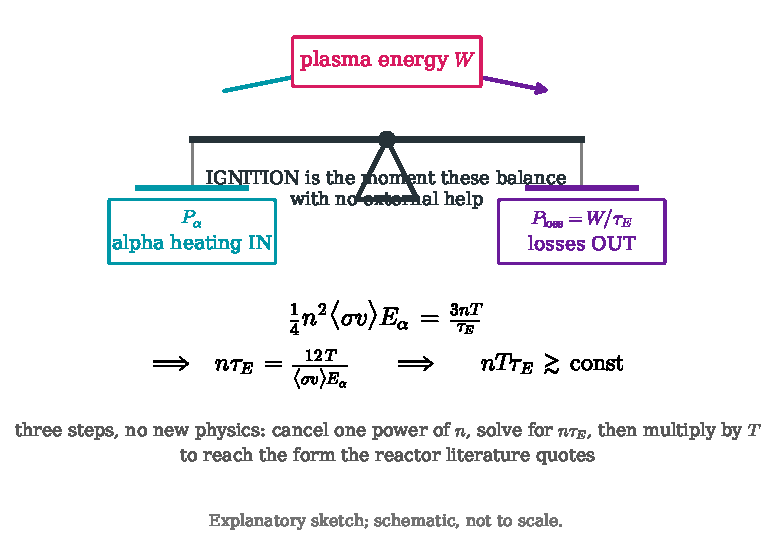
\includegraphics[width=1.0\textwidth]{figures/final/figS_ignition_balance.pdf}
  \caption{Physics sketch: the ignition balance. \schematicnote}
  \label{fig:figS_ignition_balance}
\end{figure}


\designconsequence{Ignition does not mean high temperature alone. A reactor needs a
particular combination of density, temperature, and confinement. Improving any one
of them can relax the burden on the other two, but only within their own limits.}

% ============================= PAGE 30 ==============================
\newpage
\section*{30. Gain is a ratio, not a synonym for ignition}

A plasma can make useful fusion power without being ignited if external heating
supplies the missing energy. Define the plasma gain
\begin{equation}
 Q_{\rm plasma}\equiv\frac{P_{\rm fus}}{P_{\rm aux}},
 \label{eq:qplasma}
\end{equation}
where $P_{\rm aux}$ is the heating delivered to the plasma by neutral beams, radio
frequency systems, or other actuators. In steady state, a stripped-down energy
balance is
\begin{equation}
 P_\alpha+P_{\rm aux}=P_{\rm loss}.
 \label{eq:power-balance}
\end{equation}
As $P_{\rm aux}$ tends to zero while the equality remains possible, $Q_{\rm plasma}$
tends to infinity: that limiting case is ignition. At finite $Q_{\rm plasma}$, the
plant must supply auxiliary power and also pay the inefficiency of producing and
delivering it.

The distinction protects the argument from a common mistake. A large
$Q_{\rm plasma}$ is a plasma metric. Net electric power is a plant metric that also
depends on neutron-energy capture, thermal conversion, magnet refrigeration,
pumps, controls, and all other recirculating loads. We will not declare a plant
successful from Eq.~\eqref{eq:qplasma}; we have not yet derived the components that
would make that claim meaningful.

\supportingquantity{$Q_{\rm plasma}$}{This ratio records how much fusion power is
obtained per unit of auxiliary power delivered to the plasma. It enters the later
Friedberg power ledger but cannot by itself establish net electricity.}

\designconsequence{The current ordinary-tokamak drawing has now earned auxiliary
heating but not yet a power plant. The next physical obstacle is that $\tau_E$ is
not supplied by the equilibrium equations: it is set by transport.}
% ============================= PAGE 31 ==============================
\newpage
\section*{31. Why transport is the unresolved clock}

A particle in a uniform magnetic field circles with a characteristic gyroradius
$\rho$. A collision changes the direction of its velocity; the center of the next
gyro-orbit is displaced by an amount of order $\rho$. If collisions occur at rate
$\nu$, then in time $t$ there are approximately $N=\nu t$ independent steps.
Random-walk addition gives
\[
 \langle\Delta r^2\rangle\sim N\rho^2=\nu t\rho^2.
\]
By the definition $\langle\Delta r^2\rangle\sim2Dt$ in one radial direction, the
classical cross-field diffusion estimate is
\begin{equation}
 D_{\rm cl}\sim\frac{\rho^2\nu}{2}.
 \label{eq:classical-diffusion}
\end{equation}
A container of minor radius $a$ would then have a diffusion time of order
\begin{equation}
 \tau_{\rm diff}\sim\frac{a^2}{D_{\rm cl}}.
 \label{eq:diffusion-time}
\end{equation}
This is a transparent reason strong field helps: $\rho\propto1/B$, so the classical
diffusion coefficient falls roughly as $1/B^2$ if the collision rate is held fixed.

Unfortunately, measured tokamak energy transport is frequently much faster than this
naive collisional estimate. Fluctuations and collective turbulence create correlated
motions across flux surfaces. The derivation above is therefore not a promised
confinement law. It is the baseline that tells us why the problem is surprising and
why an empirical confinement time must later enter the reactor calculation.

\imagebrief{Physics sketch: random-walk transport across flux surfaces}{Draw nested
flux surfaces with a guiding center taking many small, collision-induced radial steps
of size about $\rho$. Beside it, show the derivation
$N=\nu t$, $\langle\Delta r^2\rangle\sim N\rho^2$, and
$D_{\rm cl}\sim\rho^2\nu/2$. Label turbulence as an additional, not-yet-modelled
transport channel.}

\begin{figure}[htbp]\centering
  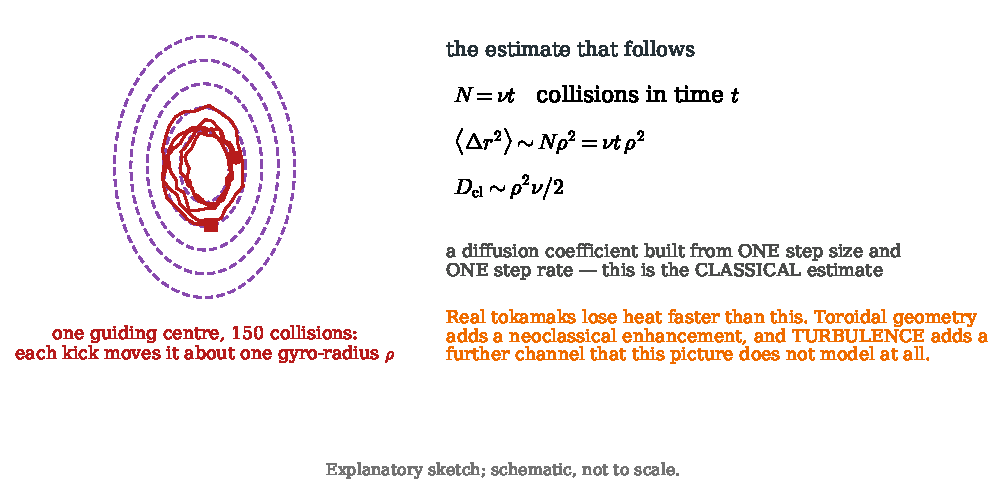
\includegraphics[width=1.0\textwidth]{figures/final/figS_random_walk.pdf}
  \caption{Physics sketch: random-walk transport across flux surfaces. \schematicnote}
  \label{fig:figS_random_walk}
\end{figure}


\designconsequence{Magnetic geometry suppresses simple cross-field diffusion, but it
does not guarantee the required $\tau_E$. A reactor design must carry a confinement
model and its uncertainty as explicitly as it carries $B_0$ or $a$.}

% ============================= PAGE 32 ==============================
\newpage
\section*{32. An empirical confinement law must be treated as data, not destiny}

For reactor studies, the working confinement time is often represented as
\begin{equation}
 \tau_E=H\,\tau_{E,\rm ref}(I_p,B_0,n,P_{\rm loss},R_0,a,\kappa,\ldots).
 \label{eq:Hfactor}
\end{equation}
Here $\tau_{E,\rm ref}$ is a regression fitted to a specified database of
experiments, and $H$ is the ratio of the observed confinement to that reference.
This equation is deliberately written without pretending that the exponents in a
particular regression are fundamental constants. The role of the formula is to make
an extrapolation auditable: which database, operating regime, units, heating mode,
and shape range were used?

The distinction between a derived equation and a fit matters especially here.
Equation~\eqref{eq:classical-diffusion} followed from a stated random-walk model.
Equation~\eqref{eq:Hfactor} is a bookkeeping identity once a reference scaling is
chosen; its predictive content lives in the data and the applicability range of
$\tau_{E,\rm ref}$. Neither should be disguised as the other.

A practical design calculation must therefore report at least three things: the
selected reference law, the assumed $H$, and a sensitivity range. If the operating
point requires $H$ well above what comparable experiments have obtained, that is not
a proof of impossibility, but it is an explicit research risk rather than hidden
optimism.

\supportingquantity{$H$}{The confinement multiplier $H$ makes the
assumption behind an empirical $\tau_E$ explicit. Friedberg-style closure cannot
treat it as a harmless fitted detail, because Eq.~\eqref{eq:lawson} makes
confinement directly load-bearing.}

\model{No universal first-principles turbulence calculation is used in this thesis
opening. When a particular confinement regression is introduced in the Friedberg
reconstruction, its published coefficient, units, database, and fit range will be
quoted alongside the calculation.}

\designconsequence{A high-field, well-shaped plasma may still fail the energy balance
if its actual transport is too fast. Confinement is not an optional correction added
after geometry; it closes the same power balance.}

% ============================= PAGE 33 ==============================
\newpage
\section*{33. Pressure cannot rise freely: the origin of a beta limit}

Before the next two named constraints appear, keep their evidence status separate.
The pressure-versus-line-bending argument below is a derived scaling. The practical
normalized-beta boundary introduced on page 34 is an empirical/model closure. The
Greenwald relation on page 35 is an empirical operating boundary. Their physical
motivation is useful; none of their numerical coefficients follows from this local
force-balance estimate alone.

The beta on page 8 compares plasma pressure with magnetic pressure:
\[
 \beta=\frac{p}{B_0^2/(2\mu_0)}.
\]
Why should there be an upper limit? Imagine a bulge of a pressure-carrying flux tube.
The pressure force trying to enlarge it scales as $p$ times its cross-sectional area.
Bending the field lines that surround it costs magnetic energy; the restoring scale is
set by $B_\theta^2/\mu_0$, where $B_\theta$ is the poloidal field that ties the
plasma current to the geometry.

Ampere's-law scale at the edge is
\[
 B_\theta\sim\frac{\mu_0I_p}{2\pi a}.
\]
Equating pressure and bending \emph{scales}, rather than claiming an exact stability
threshold, gives
\[
 p_{\max}\sim\frac{B_\theta^2}{\mu_0}
 \sim\frac{\mu_0I_p^2}{4\pi^2a^2}.
\]
Divide by $B_0^2/(2\mu_0)$ to obtain the dimensionless structural form
\begin{equation}
 \beta_{\max}\propto\left(\frac{I_p}{aB_0}\right)^2
 \quad\hbox{in this crude local balance.}
 \label{eq:beta-scale-crude}
\end{equation}
A full ideal-MHD stability calculation changes this simplified power and introduces
shape and profile dependence. The important accessible result is the mechanism:
pressure pushes outward, and magnetic line bending supplies the restoring budget.

\imagebrief{Physics sketch: pressure drive versus line bending}{Draw a small bulged
segment of a flux tube. Use outward arrows labelled pressure drive $p$ and inward
tension arrows labelled poloidal-field bending $B_\theta^2/\mu_0$. Include the
edge-field estimate $B_\theta\sim\mu_0I_p/(2\pi a)$, and state that this is a
scaling argument rather than the final MHD stability calculation.}

\begin{figure}[htbp]\centering
  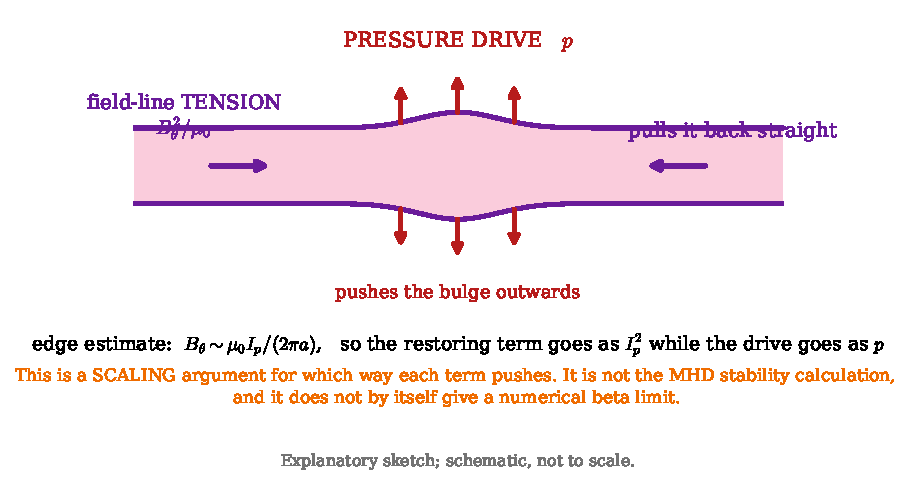
\includegraphics[width=1.0\textwidth]{figures/final/figS_pressure_vs_bending.pdf}
  \caption{Physics sketch: pressure drive versus line bending. \schematicnote}
  \label{fig:figS_pressure_vs_bending}
\end{figure}


\designconsequence{The variables desired for fusion power, $p$ and $B_0$, cannot be
optimized separately from $I_p$, shape, and stability. The next page records the
standard practical normalization of this coupled limit.}

% ============================= PAGE 34 ==============================
\newpage
\section*{34. The normalized beta used in reactor design}

Detailed ideal-MHD calculations and experiments are commonly summarized by a
normalized beta. With $\beta$ written as a fraction rather than a percentage, define
\begin{equation}
 \beta_N\equiv
 \frac{\beta\,a(\mathrm m)\,B_0(\mathrm T)}{I_p(\mathrm{MA})}.
 \label{eq:betaN}
\end{equation}
This is a convention with stated units, not a dimensionless number formed from pure
SI variables. It is useful because comparable tokamak equilibria show an approximate
operating boundary of the form
\begin{equation}
 \beta\lesssim\beta_{N,\max}
 \frac{I_p(\mathrm{MA})}{a(\mathrm m)B_0(\mathrm T)}.
 \label{eq:troyon-form}
\end{equation}
The coefficient $\beta_{N,\max}$ is empirical/model-dependent; it must be imported
from a specified stability study or design paper, never derived by dimensional
analysis alone.

Equation~\eqref{eq:troyon-form} is nevertheless more than a fit-shaped ornament.
It preserves the direction demanded by the pressure-versus-bending argument:
larger allowable current raises allowable pressure, while a larger $aB_0$ at fixed
current lowers this particular normalized beta. Combining it with the current ceiling
on page 15 makes the coupling visible: the kink limit restricts $I_p$, which then
restricts the pressure that can be claimed for fusion power.

\supportingquantity{$\beta_N$}{Normalized beta is the portable stability-performance
variable used to turn an MHD pressure limit into a reactor constraint. Its numerical
limit is a sourced assumption; its coupling to $I_p$, $a$, and $B_0$ is explicit in
Eq.~\eqref{eq:troyon-form}.}

\designconsequence{The safe operating pressure is bounded twice: directly by
pressure-driven stability and indirectly by the current that kink stability permits.
A credible design must check both bounds at the same point.}

% ============================= PAGE 35 ==============================
\newpage
\section*{35. Density has a separate experimental limit}

It would be tempting to use Eq.~\eqref{eq:plasma-pressure} and conclude that a chosen
pressure can always be obtained by trading density against temperature. Tokamak
operation does not permit an unlimited trade. A widely used experimental reference is
the Greenwald density
\begin{equation}
 n_G=
 \frac{I_p(\mathrm{MA})}{\pi a^2(\mathrm m^2)}
 \times10^{20}\ \mathrm{m^{-3}}.
 \label{eq:greenwald}
\end{equation}
Operational scenarios usually report the fraction $f_G=n_e/n_G$, rather than merely
a raw density.

There is an important methodological point here. Equation~\eqref{eq:greenwald} is
not derived from the preceding equilibrium equations. It summarizes observations
across tokamak discharges, and the physical mechanism behind its most general form is
not settled well enough to pretend otherwise. The equation belongs in the thesis
because it constrains designs; it belongs under an empirical label because its
coefficient is not a theorem.

The formula still carries useful transparent geometry. At fixed current, a smaller
cross-section raises the reference density as $1/a^2$. At fixed $a$, more current
raises it. But that same current is limited by $q_*$ and the same density contributes
to pressure and radiation. The quantity $f_G$ makes this web testable without
claiming that one line of algebra has solved the underlying edge physics.

\supportingquantity{$n_G$ and $f_G$}{The Greenwald density and its operating fraction
are empirical constraints on $n_e$. They are load-bearing whenever the fusion-power
calculation seeks higher density, and their extrapolation must be treated as an
assumption with a range.}

\imagebrief{Constraint sketch: pressure is not one knob}{Draw a three-axis conceptual
plot or linked sliders for density $n$, temperature $T$, and pressure $p=2nT$.
Overlay separate labels for the Greenwald reference $n_G$, the beta limit, and the
Lawson requirement. The point is to show that increasing $n$ affects several
constraints at once; do not imply a precise universal operating boundary.}

\begin{figure}[htbp]\centering
  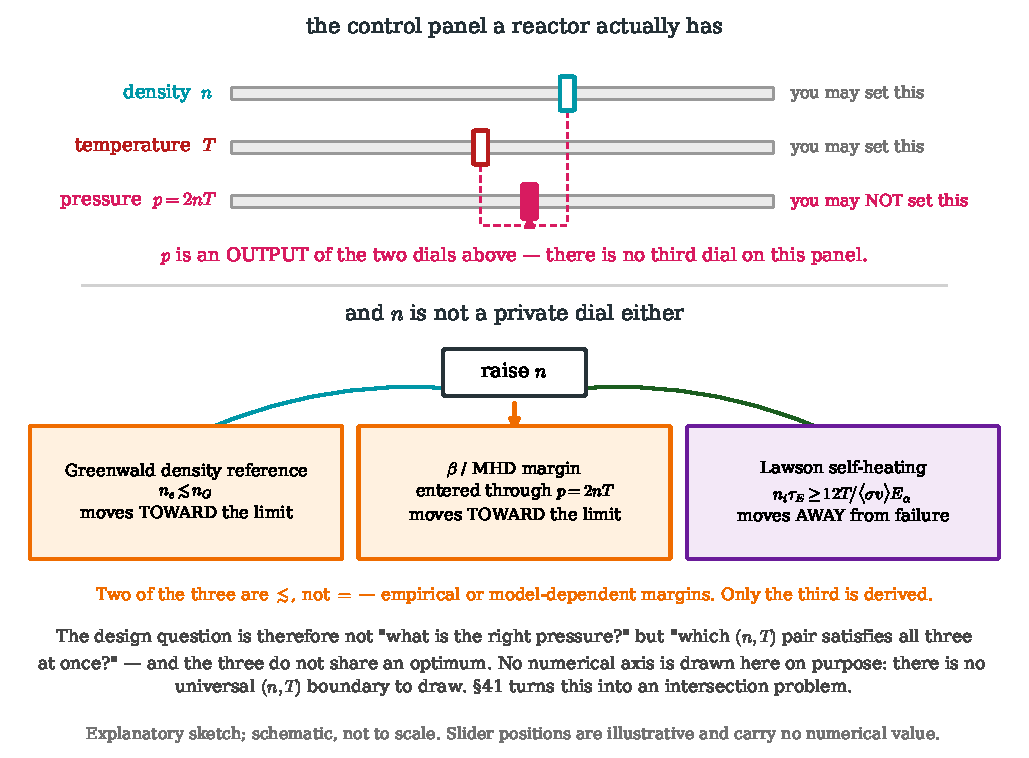
\includegraphics[width=1.0\textwidth]{figures/final/figS_pressure_not_one_knob.pdf}
  \caption{Constraint sketch: pressure is not one knob. \schematicnote}
  \label{fig:figS_pressure_not_one_knob}
\end{figure}


\designconsequence{The density needed by the fusion rate has its own operational
ceiling. A reactor must find a region that satisfies density, pressure, current, and
confinement constraints simultaneously.}

% ============================= PAGE 36 ==============================
\newpage
\section*{36. Toroidal geometry traps some particles}

The toroidal field is stronger on the inboard side because approximately
$B_\varphi\propto1/R$. A particle moving into stronger field converts parallel
motion into perpendicular motion while conserving, to lowest adiabatic order,
\[
 \mu=\frac{mv_\perp^2}{2B}
 \quad\hbox{and}\quad
 \frac12m(v_\parallel^2+v_\perp^2).
\]
Let the particle start where the field is $B_{\min}$ and let $\alpha$ be its pitch
angle there, so $v_\perp=v\sin\alpha$. At the turning point $v_\parallel=0$.
Conservation of $\mu$ gives
\[
 \frac{v^2\sin^2\alpha}{B_{\min}}=\frac{v^2}{B_{\max}},
 \qquad
 \sin^2\alpha=\frac{B_{\min}}{B_{\max}}.
\]
Particles with larger perpendicular fraction reach this condition before the high-field
side and bounce back. For isotropically distributed velocity directions, the trapped
fraction is therefore
\begin{equation}
 f_t=\sqrt{1-\frac{B_{\min}}{B_{\max}}}.
 \label{eq:trapped-fraction}
\end{equation}
This is a geometric consequence of the same $1/R$ toroidal field that was introduced
to close the open magnetic corridor. It is neither uniformly good nor uniformly bad:
trapping changes transport, and a pressure gradient acting on trapped orbits can also
produce useful self-generated current.

\supportingquantity{$f_t$}{The trapped-particle fraction in Eq.~\eqref{eq:trapped-fraction}
is a geometry-dependent input to neoclassical transport and bootstrap-current
reasoning. Here neoclassical means transport calculated from Coulomb collisions
together with the torus-specific guiding-center orbits; it is more than the
cylindrical classical-collision estimate, but it is still a stated kinetic model.
This prepares the final missing current variable without invoking any
spherical-tokamak comparison.}

\imagebrief{Physics sketch: a trapped orbit}{Show a poloidal cross-section with
stronger field on the inboard side. Draw one passing orbit and one trapped
guiding-center path, called a banana orbit because its poloidal projection has that
shape, marking two turning points where $v_\parallel=0$. Include a small inset
deriving the mirror condition from conservation of $\mu$ and energy.}

\begin{figure}[htbp]\centering
  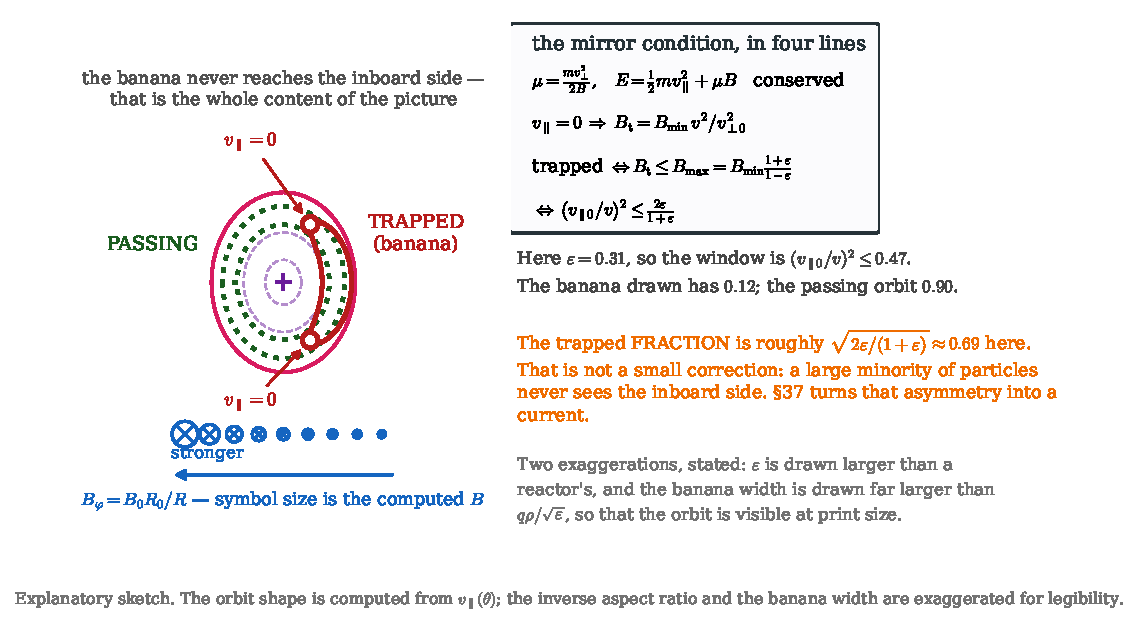
\includegraphics[width=1.0\textwidth]{figures/final/figS_trapped_orbit.pdf}
  \caption{Physics sketch: a trapped orbit. \schematicnote}
  \label{fig:figS_trapped_orbit}
\end{figure}


\designconsequence{The torus creates more than a closed corridor. Its unavoidable
field variation creates an orbit population whose asymmetry can help supply plasma
current, but only through a kinetic mechanism that must be introduced honestly.}
% ============================= PAGE 37 ==============================
\newpage
\section*{37. A pressure gradient can generate some of the required current}

A trapped particle does not sample the two sides of the torus symmetrically. Its
guiding-center drifts and collisions depend on energy and pitch angle. When pressure
falls outward, there are more energetic particles on the inner side of a local radial
interval than on the outer side. The resulting imbalance in trapped-particle motion is
communicated by collisions to passing electrons. The outcome is a net toroidal current
called the \emph{bootstrap current}.

The direction and detailed coefficient require kinetic theory, because they depend on
collisions, geometry, temperature gradients, and the current profile. What can be
stated before importing such a coefficient is the structure:
\begin{equation}
 j_{\rm bs}\propto-\frac{dp}{dr}
 \quad\hbox{and}\quad
 I_{\rm bs}=\int j_{\rm bs}\,dA.
 \label{eq:bootstrap-structure}
\end{equation}
No pressure gradient means no bootstrap drive in this simplified statement. A steeper
gradient can produce more self-driven current, but it also moves the plasma closer to
pressure-driven stability limits. The word bootstrap should therefore not be heard as
free current. It is a coupling between the profile needed for confinement and the
current needed for magnetic geometry.

Define the bootstrap fraction
\begin{equation}
 f_{\rm bs}\equiv\frac{I_{\rm bs}}{I_p}.
 \label{eq:bootstrap-fraction}
\end{equation}
A later kinetic model can supply a coefficient and a profile-dependent prediction for
$f_{\rm bs}$. At this stage, the variable is already essential because it reduces the
current that must be supplied by a transformer or external current drive.

\friedbergvariable{$f_B$ (bootstrap fraction)}{Here $f_B$ is written
$f_{\rm bs}=I_{\rm bs}/I_p$ in Eq.~\eqref{eq:bootstrap-fraction}. It is the
self-generated share of the required plasma current. Its numerical value must come
from a cited kinetic model or experiment, not from the proportionality sign alone.}

\model{Equation~\eqref{eq:bootstrap-structure} is a mechanism and sign statement,
not a complete bootstrap-current formula. The later Friedberg reconstruction will
identify exactly which neoclassical coefficient it uses and will keep its profile
assumptions visible.}

\designconsequence{The pressure profile can help sustain the magnetic geometry, but
it cannot be assigned independently of the stability and confinement requirements
that created the profile in the first place.}

% ============================= PAGE 38 ==============================
\newpage
\section*{38. The full current ledger}

The toroidal plasma current can have several sources. Write the accounting identity
\begin{equation}
 I_p=I_{\rm ohm}+I_{\rm CD}+I_{\rm bs}.
 \label{eq:current-ledger}
\end{equation}
The first term is transformer-induced ohmic current; it is available while the
central solenoid changes linked flux. The second is externally driven non-inductive
current, for example from waves or beams transferring directed momentum. The third
is the pressure-gradient-driven bootstrap current from page 37.

This equation is not a performance claim. It is a definition of what must be
accounted for. For a long pulse after transformer action has faded,
$I_{\rm ohm}\simeq0$, and Eq.~\eqref{eq:current-ledger} reduces to
\begin{equation}
 I_{\rm CD}=(1-f_{\rm bs})I_p.
 \label{eq:current-drive-need}
\end{equation}
The larger the bootstrap fraction, the smaller the externally driven current
requirement. But current drive consumes power and its efficiency depends on density,
temperature, magnetic field, launch geometry, and the actuator itself. A design may
not set $f_{\rm bs}$ near one merely to make the accounting easy.

\supportingquantity{$I_{\rm CD}$}{Equation~\eqref{eq:current-drive-need} makes the
unself-driven current explicit. It is the quantity later translated into heating and
recirculating-power demand; it links plasma profiles to plant power balance.}

\imagebrief{Cumulative construction state 11: the current ledger on the machine}{Start
with the shaped conventional tokamak. Keep the central solenoid, heating/current-drive
ports, and profile inset. Add a compact ledger beside the plasma:
$I_p=I_{\rm ohm}+I_{\rm CD}+I_{\rm bs}$. Use arrows from the solenoid, an auxiliary
port, and the pressure-gradient/profile inset to the three terms. Do not draw
engineering components that have not yet been derived.}

\begin{figure}[htbp]\centering
  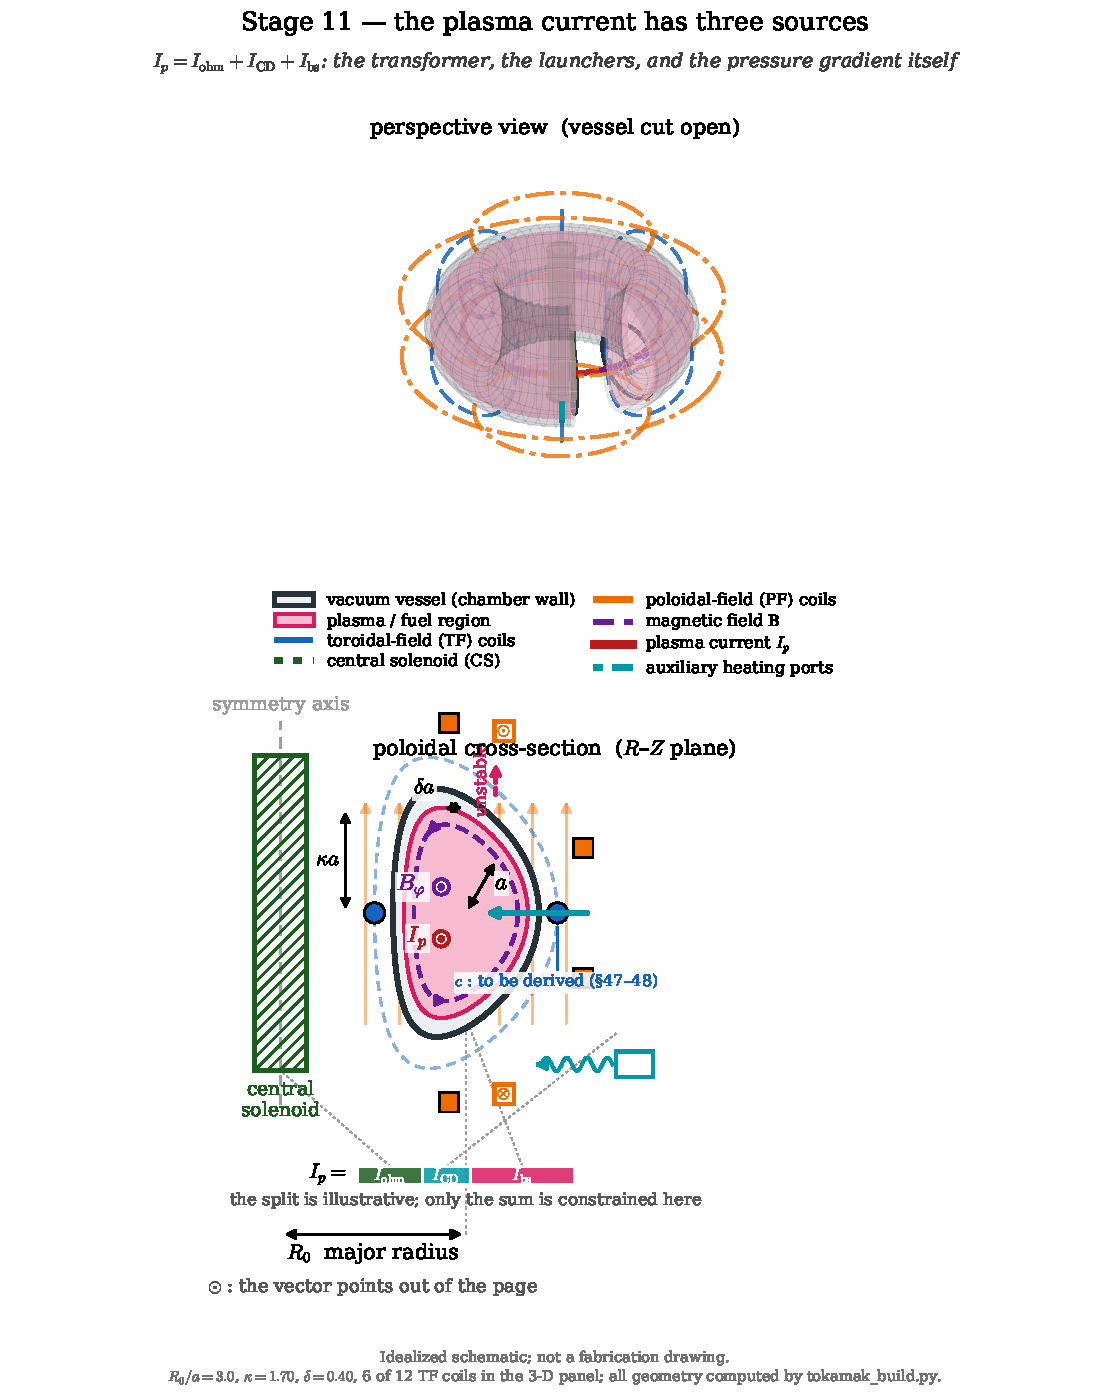
\includegraphics[width=1.0\textwidth]{figures/final/figM11_stage11_tall.pdf}
  \caption{Machine state: the full current ledger, $I_p=I_{\rm ohm}+I_{\rm CD}+I_{\rm bs}$, drawn as a stacked bar because the three terms add. The split shown is illustrative; only the sum is constrained at this point.}
  \label{fig:figM11_stage11_tall}
\end{figure}


\designconsequence{Steady operation is a three-way closure: the current required by
$q_*$ must be consistent with the bootstrap current predicted by profiles and the
external current-drive power the plant can afford.}

% ============================= PAGE 39 ==============================
\newpage
\section*{39. Pulsed operation is also a legitimate design choice}

The central solenoid is a transformer primary. Faraday's law gives the loop voltage
around the torus:
\[
 \oint\mathbf E\cdot d\boldsymbol\ell=-\frac{d\Phi_{\rm link}}{dt}.
\]
For a torus of major radius $R_0$, a representative toroidal electric field satisfies
$2\pi R_0E_\varphi=-d\Phi_{\rm link}/dt$. The solenoid has a finite usable flux swing
$\Delta\Phi_{\rm link}$, so it can induce current only for a finite time. This is the
physical origin of the transformer clock introduced on page 11.

There are two coherent responses. One is a pulsed plant: use transformer current
during a burn, then recharge the solenoid between pulses. The other is a long-pulse
or steady-state plant: replace the lost ohmic contribution with the current-drive and
bootstrap terms in Eq.~\eqref{eq:current-ledger}. Neither option is free. Pulsing
creates thermal cycling and dwell-time questions; non-inductive operation creates
actuator power and accessibility questions. The correct choice belongs to an
integrated design, not to a slogan about steady state.

\supportingquantity{$\Delta\Phi_{\rm link}$}{The available linked-flux swing is the
pulsed-operation resource. It sets how much transformer action the central solenoid
can provide before the current ledger must rely on non-inductive sources.}

\imagebrief{Physics sketch: two ways to close the current ledger}{Make a two-panel
conceptual diagram. Left: a pulsed timeline with solenoid flux decreasing during a
burn and recharging during dwell. Right: a long-pulse balance with
$I_{\rm CD}+I_{\rm bs}$ replacing $I_{\rm ohm}$. Keep it a clean accounting sketch,
not a claim that either architecture is automatically preferable.}

\begin{figure}[htbp]\centering
  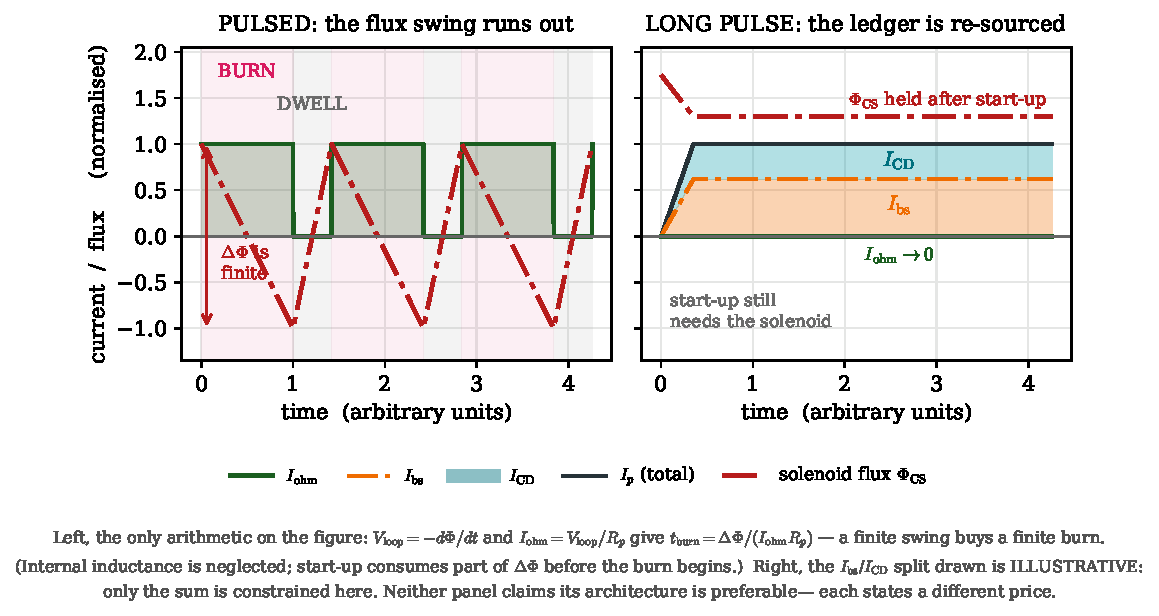
\includegraphics[width=1.0\textwidth]{figures/final/figS_close_the_ledger.pdf}
  \caption{Physics sketch: two ways to close the current ledger. \schematicnote}
  \label{fig:figS_close_the_ledger}
\end{figure}


\designconsequence{The central solenoid has earned a place in the ordinary tokamak,
but it also creates a choice between pulse duration, stored flux, and non-inductive
current-drive burden. That choice will become an explicit Friedberg assumption.}

% ============================= PAGE 40 ==============================
\newpage
\section*{40. The kink limit returns as a constraint on every current source}

The current ledger does not allow arbitrary total current. A helical disturbance can
be labelled by integers $(m,n)$ through a displacement pattern
$\xi\propto\cos(m\theta-n\varphi)$. Along an unperturbed field line, a poloidal turn
changes $\theta$ by $2\pi$ while the toroidal angle changes by $2\pi q$. The phase
change is therefore $2\pi(m-nq)$. When $q=m/n$, the disturbance remains in phase
after a circuit; field-line bending has the least geometric leverage to average it
away.

This is the accessible reason safety factor is a stability variable rather than only
a geometric ratio. The full ideal-MHD energy principle determines the precise
stability boundary. Reactor studies commonly use a specified global constraint
\begin{equation}
 q_*>q_K,
 \label{eq:kink-constraint-repeat}
\end{equation}
with $q_K$ supplied by the chosen stability model. Substituting the shaped
safety-factor formula, Eq.~\eqref{eq:qstar}, reproduces the current ceiling already
derived in Eq.~\eqref{eq:ip-kink-limit}. Every term in the current ledger must fit
under that same ceiling; bootstrap current helps meet a required $I_p$ but does not
abolish the stability constraint on $I_p$ itself.

\supportingquantity{$q_K$}{The kink threshold is a stability-model input applied to
the shaped safety factor. It converts an otherwise desirable current into an upper
bound and must be stated whenever a reactor calculation quotes $I_p$.}

\model{This page derives the resonance logic, not the full numerical value of $q_K$.
The later reconstruction will distinguish the analytical Kruskal--Shafranov
criterion from the practical design threshold used in the 2015 paper.}

\designconsequence{Current-drive accounting and kink stability are the same problem
viewed from two directions: one asks where $I_p$ comes from; the other asks how much
total $I_p$ the plasma can safely carry.}

% ============================= PAGE 41 ==============================
\newpage
\section*{41. The operating point is an intersection, not a target number}

We can now state the first coupled operating-space problem without claiming to have
solved it. A candidate state must satisfy, at minimum,
\begin{align}
 q_*&>q_K &&\text{current and kink margin},\label{eq:wall-q}\\
 \beta&\lesssim\beta_{N,\max}\frac{I_p}{aB_0}
 &&\text{pressure and MHD margin},\label{eq:wall-beta}\\
 n_e&\lesssim n_G &&\text{density reference},\label{eq:wall-density}\\
 n_i\tau_E&\ge\frac{12T}{\langle\sigma v\rangle E_\alpha}
 &&\text{self-heating requirement},\label{eq:wall-lawson}\\
 I_p&=I_{\rm ohm}+I_{\rm CD}+I_{\rm bs}
 &&\text{current accounting}.\label{eq:wall-current}
\end{align}
The notation $\lesssim$ in the second and third lines is deliberate. Those limits
are modelled or empirical margins, not exact equalities. The last line is an
identity, but its terms depend on operating mode and profiles. The first and fourth
lines are inequalities derived from explicit physical balances, with a stability
threshold or reactivity curve still to be specified.

This set is why the thesis refuses to present a tokamak as a collection of parts.
Increasing density might help Eq.~\eqref{eq:wall-lawson} but challenge
Eq.~\eqref{eq:wall-density}; increasing current can improve one normalized beta
bound but challenge Eq.~\eqref{eq:wall-q}; improving confinement changes needed
heating and current drive. The correct question is whether the inequalities overlap
with usable margin.

\imagebrief{Constraint-map sketch: the ordinary tokamak operating window}{Create a
schematic, clearly labelled overlap diagram rather than a numerically calibrated plot.
Show five boundaries corresponding to Eqs.~\eqref{eq:wall-q}--\eqref{eq:wall-current}
and one small shaded feasible region. Include a warning that the plot is conceptual
until a named confinement scaling, stability model, and profile model are supplied.}

\begin{figure}[htbp]\centering
  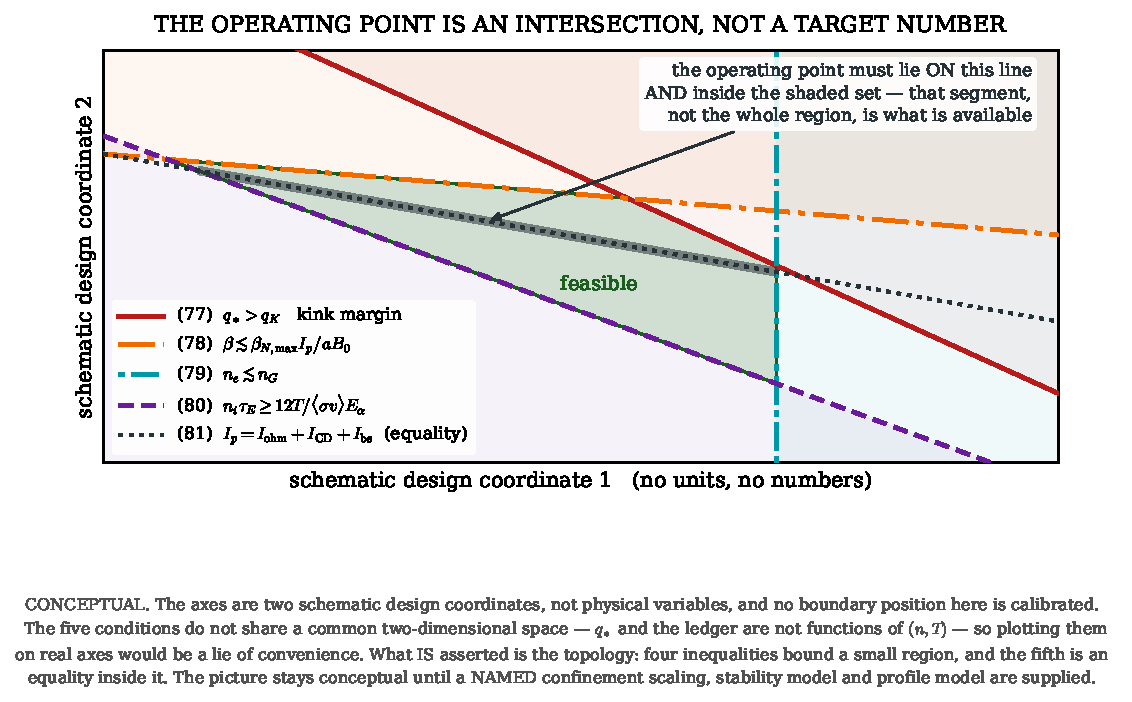
\includegraphics[width=1.0\textwidth]{figures/final/figS_operating_window.pdf}
  \caption{Constraint-map sketch: the ordinary tokamak operating window. \schematicnote}
  \label{fig:figS_operating_window}
\end{figure}


\designconsequence{The next stage is not to add more variables randomly. It is to
take the exact set just derived and reconstruct, line by line, how Friedberg's 2015
reference design attempts to close it.}

% ============================= PAGE 42 ==============================
\newpage
\section*{42. The primary parameter set is not complete yet}

The conventional tokamak has appeared in a causal order. Fusion temperature required a nonmaterial
container. Charged particles made magnetic steering possible. Open field lines forced
the torus and TF coils; drifts and pressure forced the plasma current, central solenoid,
PF coils, and shaped equilibrium; transformer limits and power balance forced heating,
current drive, and the distinction between pulsed and non-inductive operation. Shape
was added only after its geometric and control price was visible.

The canonical target is Friedberg's Table-1 set,
\[
 a,\ R_0,\ \kappa,\ b,\ c,\ T,\ n,\ p,\ \tau_E,\ B_0,\ \beta,\ I,\ q_*,\ f_B.
\]
This draft has derived the physical role of $a,R_0,\kappa,T,n,p,\tau_E,B_0,\beta$,
$I$, $q_*$, and $f_B$. It has deliberately also introduced supporting quantities---
for example $A,\delta,q(r),\beta_N,H,I_{\rm CD}$, and $Q_{\rm plasma}$---because
they make the causal argument intelligible. They are not additional primary
Friedberg parameters or automatically independent design knobs. The two missing
Table-1 hardware parameters are $b$ (blanket-region thickness) and $c$
(TF-magnet thickness). They must earn their place before numerical Friedberg closure
begins.

\supportingquantity{remaining Part-I task}{The next physical chain is neutron escape
to first wall, blanket, shielding, and then the TF magnet. It must explain why the
blanket-region thickness $b$ and TF-magnet thickness $c$ are indispensable primary
parameters before the 2015 numerical reactor argument is reconstructed.}

\imagebrief{Construction-atlas checkpoint: before the nuclear island}{Update
the cumulative conventional-tokamak atlas through state 11. Add a margin legend
linking each physical component to its derived variable: TF coils to $B_0$; solenoid
to $\Delta\Phi_{\rm link}$ and $I_{\rm ohm}$; PF coils to $\kappa,\delta,\psi$;
plasma to $p,n,T,I_p,q$; heating/current-drive ports to $P_{\rm aux},I_{\rm CD}$;
and feedback to vertical control. Leave a labelled future radial-space budget for
first wall, blanket region $b$, shield, and TF-magnet thickness $c$; do not draw
them as completed components yet. Exclude spherical-tokamak geometry.}

\begin{figure}[htbp]\centering
  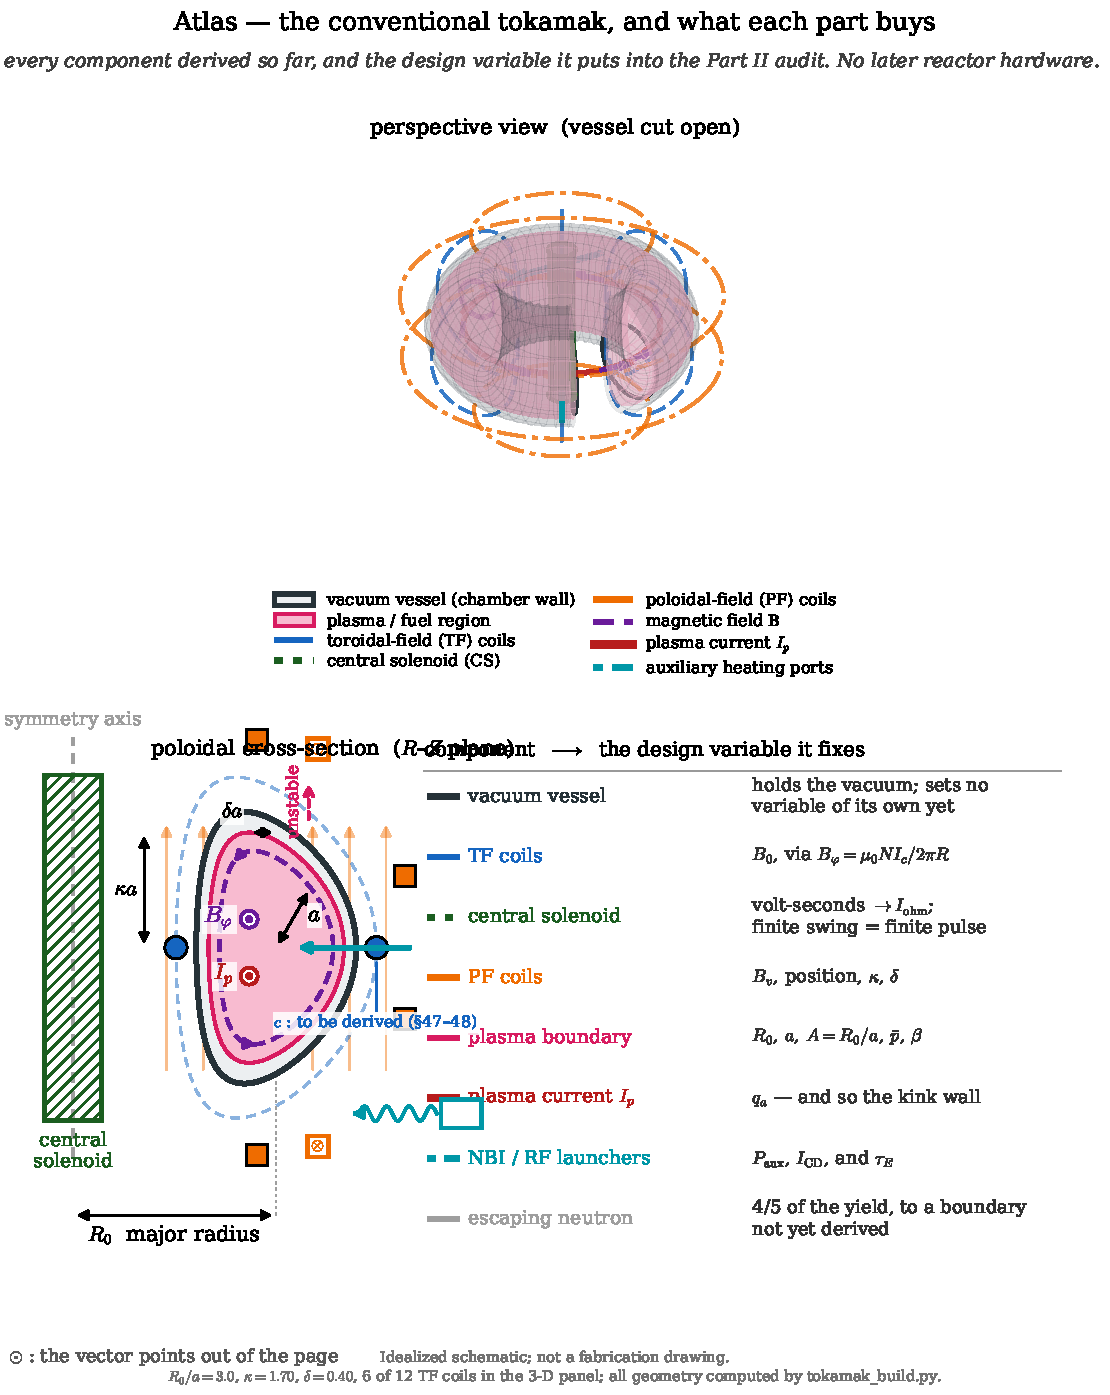
\includegraphics[width=1.0\textwidth]{figures/final/figM12_stage12_tall.pdf}
  \caption{Atlas. Every component derived so far, and the design variable each one puts into the audit that follows. No later reactor hardware appears.}
  \label{fig:figM12_stage12_tall}
\end{figure}


\designconsequence{Before calculating a reactor, the next pages must derive the
nuclear island and the toroidal-field-magnet thickness. Only after $b$ and $c$ have
joined the same causal parameter set can the thesis begin Friedberg's numerical
engineering-and-nuclear-physics closure.}
% ============================= PAGE 43 ==============================
\newpage
\section*{43. A magnetic bottle does not catch the neutron}

The D--T reaction in Eq.~\eqref{eq:dt} has two products with very different fates.
The charged alpha particle remains magnetically guided and can transfer energy back to
the plasma. The neutron has no electric charge. Its Lorentz force is exactly zero:
\[
 \mathbf F_n=0\cdot(\mathbf E+\mathbf v_n\times\mathbf B)=0.
\]
It leaves the magnetic surfaces in a nearly straight line and reaches the first
material it encounters. This is not an engineering inconvenience added after the
plasma is designed. It is an unavoidable consequence of choosing the D--T reaction.

The neutron carries $14.1\,\mathrm{MeV}$, approximately four fifths of the fusion
energy. A power-producing machine must therefore do four jobs outside the plasma:
survive the first impact, slow and capture neutrons, breed replacement tritium, and
protect the magnets and vacuum boundary from the remaining radiation. These jobs
force a radial region between plasma and TF coil. We call its total inboard/outboard
thickness $b$.

\friedbergvariable{$b$ (blanket-region thickness)}{The D--T neutron is neutral, so
magnetic confinement cannot retain it. A reactor must reserve radial space for a first
wall, neutron multiplier or moderator where used, tritium-breeding material, shielding,
and a vacuum boundary. The parameter $b$ records the total required radial build of
this nuclear island. It is not an arbitrary clearance and it is not, by itself, a
complete blanket design.}

\imagebrief{Reset physics sketch: charged alpha versus neutral neutron}{At manuscript
state 12, show the same D--T reaction at the plasma edge. The $3.5\,\mathrm{MeV}$
alpha follows a curved magnetic guiding path back into the plasma; the
$14.1\,\mathrm{MeV}$ neutron travels straight across magnetic field lines toward a
not-yet-detailed radial material stack. Label "magnetic field does not act on a
neutral." Keep all previously earned conventional-tokamak components visible only
where needed for orientation.}

\begin{center}\small\itshape
This brief asks for the same D--T reaction that cumulative state~10 already shows in Figure~\ref{fig:figM10_stage10_tall} --- charged alpha retained, neutral neutron leaving toward a boundary not yet drawn. Under the standing rule that redundancy is fixed rather than expanded, no second figure is drawn; the two quantities this brief would add (the mass-ratio energy split and the alpha gyro-radius) belong in the prose or in that figure's caption.
\end{center}


\designconsequence{A fusion reactor is not merely a plasma plus magnets. The neutron
forces a nuclear island, and that island consumes radial space precisely where a
toroidal-field coil would prefer to be close to the plasma.}

\model{We use an intentionally simple, one-dimensional neutron model to derive the
meaning and scale of $b$. Real blanket design requires material-specific transport,
heat removal, structural design, activation analysis, and tritium-accounting margins.
Those are later engineering calculations, not facts we may silently hide in one number.}

% ============================= PAGE 44 ==============================
\newpage
\section*{44. Why the nuclear island has a thickness}

First consider the slowing-down part of the problem. In a homogeneous material with
target number density $N$ and an effective interaction cross section $\sigma_s$, the
mean distance between relevant collisions is
\begin{equation}
 \lambda_s=\frac{1}{N\sigma_s}.
 \label{eq:mean-free-path}
\end{equation}
This follows directly from probability. In a thin distance $dx$, a neutron has
collision probability $N\sigma_sdx=dx/\lambda_s$. Thus the chance of no collision
decreases exponentially with distance.

For a transparent first model, suppose each collision removes a fixed fraction $\xi$
of the neutron energy on average. Over many collisions, the average energy loss per
distance can be represented by
\begin{equation}
 \frac{dE}{dx}=-\frac{\xi E}{\lambda_s}.
 \label{eq:slowing-down}
\end{equation}
Separating variables gives
\[
 \frac{dE}{E}=-\frac{\xi\,dx}{\lambda_s}
 \quad\Longrightarrow\quad
 E(x)=E_0\exp\!\left(-\frac{\xi x}{\lambda_s}\right).
\]
To reduce a $14.1\,\mathrm{MeV}$ neutron from $E_0$ to a chosen capture-friendly
energy $E_c$, the associated slowing-down distance is therefore
\begin{equation}
 b_{\rm slow}=\frac{\lambda_s}{\xi}\ln\!\left(\frac{E_0}{E_c}\right).
 \label{eq:bslow}
\end{equation}
The logarithm matters: a large energy ratio does not require a proportional thickness,
but it does require several interaction lengths. Equation~\eqref{eq:bslow} already
shows why a thin wall cannot be a reactor solution.

Now consider breeding. One useful reaction is
\[
 n+{}^6\mathrm{Li}\longrightarrow{}^4\mathrm{He}+{}^3\mathrm{H}
 +4.8\,\mathrm{MeV}.
\]
The emitted tritium replaces fuel consumed by D--T fusion. If slow neutrons are
absorbed with macroscopic probability per length $\Sigma_B=N_6\sigma_B$, their
surviving flux $\Gamma$ obeys
\[
 \frac{d\Gamma}{dx}=-\Sigma_B\Gamma,
 \qquad
 \Gamma(x)=\Gamma(0)e^{-x/\lambda_B},
 \qquad
 \lambda_B=\frac1{\Sigma_B}.
\]
Capturing a chosen fraction $f_{\rm cap}$ then requires
\begin{equation}
 b_{\rm breed}=-\lambda_B\ln(1-f_{\rm cap}).
 \label{eq:bbreed}
\end{equation}
Both $\lambda_s$ and $\lambda_B$ depend on material and neutron energy. Thus
Eqs.~\eqref{eq:bslow}--\eqref{eq:bbreed} derive a physical requirement, not a
material-independent numerical answer.

\supportingquantity{neutron mean free path}{The quantities $\lambda_s$ and
$\lambda_B$ are supporting transport lengths, not Primary Friedberg parameters. They
explain why the primary radial-build parameter $b$ cannot be taken arbitrarily small.}

% ============================= PAGE 45 ==============================
\newpage
\section*{45. From microscopic collisions to the reactor dimension $b$}

The nuclear island is a sequence of functions, not a single substance. At the level
needed for a first reactor layout, write
\begin{equation}
 b=b_{\rm FW}+b_{\rm mult}+b_{\rm slow}+b_{\rm breed}
   +b_{\rm shield}+b_{\rm vac}.
 \label{eq:blanket-build}
\end{equation}
Here $b_{\rm FW}$ is the first-wall allowance; $b_{\rm mult}$ represents any
neutron-multiplying region; $b_{\rm slow}$ and $b_{\rm breed}$ are motivated by the
preceding transport calculation; $b_{\rm shield}$ protects coils and surrounding
structures; and $b_{\rm vac}$ is the vacuum-boundary allowance. Some concepts combine
or reorder these functions. Equation~\eqref{eq:blanket-build} is deliberately a
functional ledger, not a claim that every reactor has six sharply separated layers.

The first wall also sees a power-density demand. In the large-aspect-ratio circular
approximation, a torus with major radius $R_0$ and minor radius $a$ has surface area
\[
 S_{\rm wall}\simeq (2\pi R_0)(2\pi a)=4\pi^2R_0a.
\]
If $P_n$ is the neutron power and $W_n$ is an allowed average neutron wall loading,
\begin{equation}
 \frac{P_n}{4\pi^2R_0a}\le W_n
 \qquad\Longrightarrow\qquad
 R_0a\ge\frac{P_n}{4\pi^2W_n}.
 \label{eq:wall-loading-geometry}
\end{equation}
Elongation and detailed surface shape modify this estimate; they do not remove its
message. At fixed fusion-neutron power, a smaller first-wall area means a harsher wall
loading. Nuclear performance therefore couples the two plasma dimensions $R_0$ and
$a$ even before we make a plasma-transport calculation.

The more immediate geometric consequence of $b$ is radial crowding. On the inboard
side, the blanket lies between the plasma edge and the TF coil. It displaces the coil
toward the symmetry axis, where a toroidal field is stronger. The next section turns
that qualitative statement into an equation.

\imagebrief{Cumulative construction state 12: the earned nuclear island}{Update the
atlas with the plasma, vacuum region, first wall, blanket/breeding region, shield, and
vacuum boundary as a radial stack. Use a bracket labelled $b$ for the complete
first-wall-to-vacuum-boundary build; do not label a single inner layer as $b$. Show
one neutral-neutron path depositing energy and one tritium-breeding reaction. Retain
the already-earned TF coil as a solid component, but annotate its radial bracket as
$c$: thickness derived next, rather than assigning it a thickness. Exclude
spherical-tokamak geometry and a divertor.}

\begin{figure}[htbp]\centering
  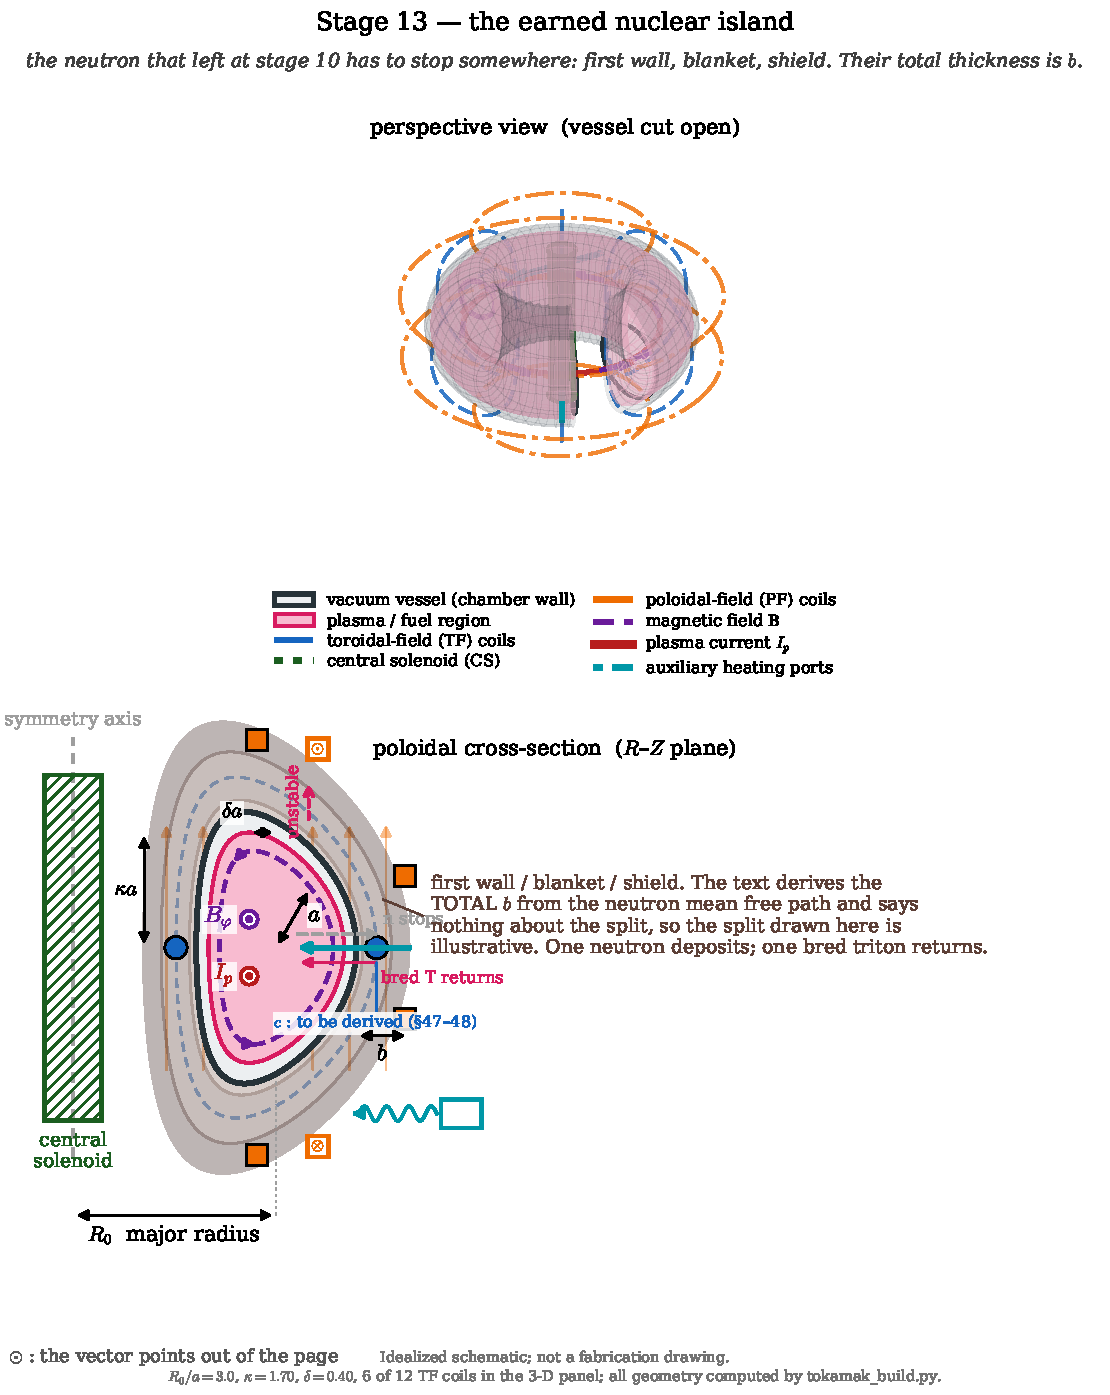
\includegraphics[width=1.0\textwidth]{figures/final/figM13_stage13_tall.pdf}
  \caption{Machine state: the earned nuclear island. The neutron that left has to stop somewhere --- first wall, blanket, shield. Their total thickness is $b$. No layer split is asserted beyond what the text derives.}
  \label{fig:figM13_stage13_tall}
\end{figure}


\designconsequence{The blanket thickness $b$ has become a geometric actor. It sets a
minimum separation between the fusion plasma and the field-producing magnet; it cannot
be optimized independently of $R_0$, $a$, $B_0$, and the eventual coil thickness $c$.}

% ============================= PAGE 46 ==============================
\newpage
\section*{46. The field gets stronger as the coil moves inward}

The continuous-coil model already gave
\[
 B_\varphi(R)=\frac{\mu_0NI_c}{2\pi R}.
\]
At the plasma centre $R=R_0$, write this as $B_0$. The inboard edge of the
plasma is at $R_0-a$. After the nuclear island and an inboard TF-coil build have been
added, the innermost high-field location lies approximately at
\begin{equation}
 R_{\rm in}=R_0-a-b-c.
 \label{eq:rin}
\end{equation}
The sign is important: moving inward means decreasing $R$, which increases the
toroidal field for fixed coil current.

Using $B_\varphi(R)R=B_0R_0$, the maximum field in this simplified radial build is
\begin{equation}
 B_{\max}=\frac{B_0R_0}{R_0-a-b-c}.
 \label{eq:bmax}
\end{equation}
Equivalently,
\begin{equation}
 B_0=B_{\max}\left(1-\frac{a+b+c}{R_0}\right).
 \label{eq:b0radialbuild}
\end{equation}
This is the first compact expression of the radial-build problem. A larger plasma
minor radius, a thicker nuclear island, or a thicker TF coil leaves less inboard
radius. At fixed material limit $B_{\max}$, each reduces the attainable central field
$B_0$.

\supportingquantity{inboard radial-build fraction}{It is often convenient to define
$\epsilon_{\rm build}=(a+b+c)/R_0$. It is a derived bookkeeping ratio, not another
primary parameter. Equation~\eqref{eq:b0radialbuild} says simply
$B_0=B_{\max}(1-\epsilon_{\rm build})$.}

The equation also explains why a tokamak cannot be designed by choosing a desirable
$B_0$ and adding the blanket and magnets afterwards. Those supposedly external
components feed back directly into the field available to the plasma.

\imagebrief{Reset geometry sketch: why inboard build limits central field}{Draw a
horizontal midplane cut through a conventional tokamak. Mark, from the plasma centre
inward: $a$, the full nuclear-island bracket $b$, the TF-coil bracket $c$, and
$R_{\rm in}=R_0-a-b-c$. Show toroidal-field arrows with increasing density inward.
Place Eqs.~\eqref{eq:bmax} and \eqref{eq:b0radialbuild} beside the sketch.}

\begin{figure}[htbp]\centering
  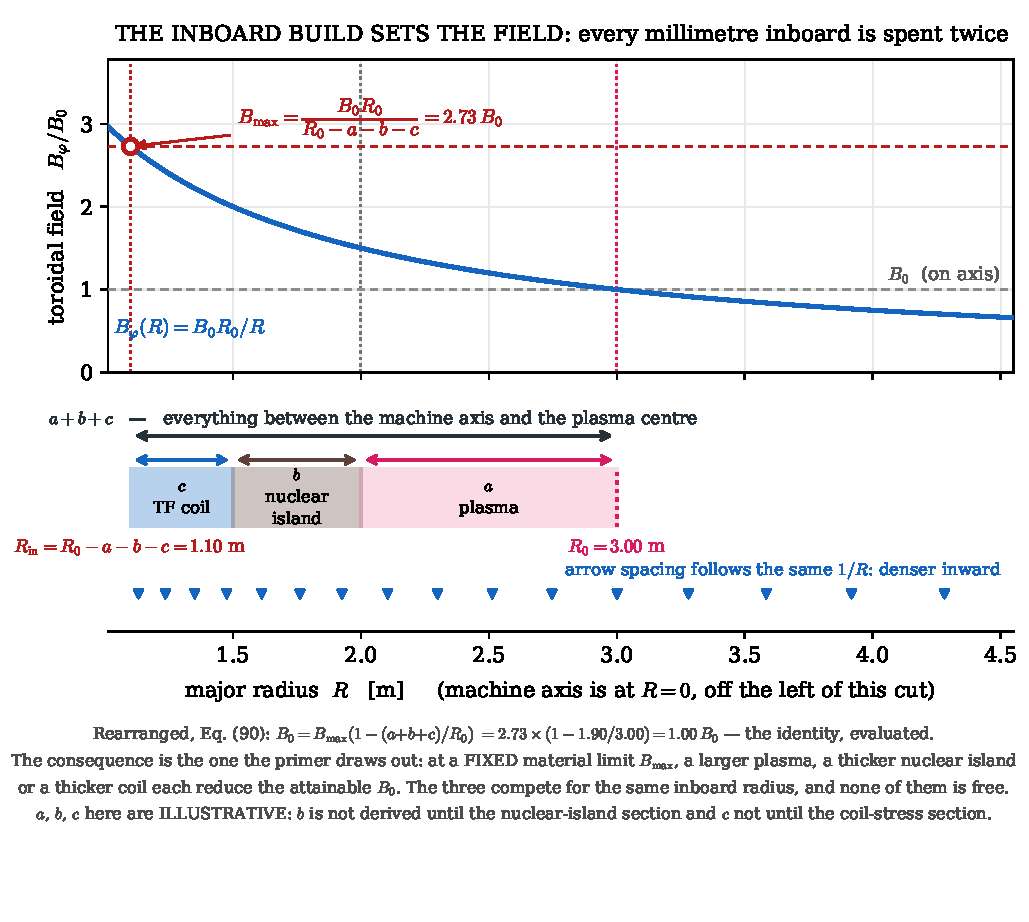
\includegraphics[width=1.0\textwidth]{figures/final/figS_inboard_build.pdf}
  \caption{Reset geometry sketch: why inboard build limits central field. \schematicnote}
  \label{fig:figS_inboard_build}
\end{figure}


% ============================= PAGE 47 ==============================
\newpage
\section*{47. A field coil must carry current and survive its own force}

A magnetic field stores energy. In vacuum its energy density is
\begin{equation}
 u_B=\frac{B^2}{2\mu_0}.
 \label{eq:magnetic-energy-density}
\end{equation}
One way to obtain this expression is to build a solenoid gradually. Its magnetic
energy is $U=\tfrac12LI^2$; dividing by volume and substituting the ideal-solenoid
relations $L=\mu_0N^2A/\ell$ and $B=\mu_0NI/\ell$ gives
$U/(A\ell)=B^2/(2\mu_0)$.

The same scale appears as a magnetic pressure. If a field-filled region expands by a
small volume $dV$ at fixed flux, the released magnetic energy supplies mechanical
work $p_BdV$. The resulting stress scale is
\begin{equation}
 p_B=\frac{B^2}{2\mu_0}.
 \label{eq:magnetic-pressure}
\end{equation}
At high field this is enormous: the dependence is quadratic, so doubling field
quadruples this stress scale. A TF coil is therefore not just superconducting cable.
It needs a structural load path that prevents the winding pack from being crushed,
pulled apart, or driven beyond allowable strain.

For a transparent thickness estimate, let a representative magnetic force be
$F\sim p_BA_{\rm load}$ and let structural material of cross-sectional area
$A_{\rm str}$ be limited to stress $\sigma_{\rm allow}$. Force balance requires
\[
 \sigma_{\rm allow}A_{\rm str}\gtrsim p_BA_{\rm load}.
\]
If the geometry converts these areas into a representative support length $\ell_s$,
then the structural contribution obeys the scaling
\begin{equation}
 c_{\rm str}\sim
 \frac{B_{\max}^2}{2\mu_0\sigma_{\rm allow}}\,\ell_s
 \times(\hbox{geometry factor}).
 \label{eq:cstructure-scaling}
\end{equation}
The geometry factor is not a nuisance to be discarded: detailed TF-coil engineering
calculates it from tensile, centering, bending, and wedging loads. Equation
\eqref{eq:cstructure-scaling} is the load-bearing physical reason that the parameter
$c$ exists at all.

\model{This section establishes the stress scaling, not a certified coil design.
Real designs use three-dimensional force analysis, material allowables at operating
temperature and fluence, insulation and cooling channels, joints where applicable,
fatigue limits, and safety margins.}

% ============================= PAGE 48 ==============================
\newpage
\section*{48. The other part of coil thickness: enough current-carrying area}

Stress is not the only reason a coil occupies space. Amp\`ere's law requires a total
enclosed current approximately
\begin{equation}
 NI\simeq\frac{2\pi R_{\rm in}B_{\max}}{\mu_0}.
 \label{eq:tf-ampere-turns}
\end{equation}
The product $NI$, called ampere-turns, cannot be carried through zero area. If
$J_{\rm wp}$ is the allowed current density averaged over the complete winding pack
(conductor, stabilizer, insulation, cooling paths, and structural allocation), the
required current-carrying area scales as
\begin{equation}
 A_{\rm wp}\gtrsim\frac{NI}{J_{\rm wp}}.
 \label{eq:winding-area}
\end{equation}
For a representative coil height $h_{\rm wp}$, this yields a winding-pack thickness
scale
\begin{equation}
 c_{\rm wp}\sim\frac{2\pi R_{\rm in}B_{\max}}
 {\mu_0J_{\rm wp}h_{\rm wp}}.
 \label{eq:winding-thickness}
\end{equation}
This is a scaling estimate, not a prescription for the cross-sectional shape of a
real coil. Its purpose is to expose the independent current-density reason that coil
thickness cannot be wished away.

The full primary parameter is therefore a radial ledger:
\begin{equation}
 c=c_{\rm str}+c_{\rm wp}+c_{\rm ins}+c_{\rm cool}+c_{\rm margin}.
 \label{eq:coil-build}
\end{equation}
The final three terms acknowledge insulation, cooling, manufacturing tolerances, and
design margin. Their values must come from an explicit technology model. The first two
terms, Eqs.~\eqref{eq:cstructure-scaling} and \eqref{eq:winding-thickness}, are the
two irreducible physical demands: survive the field and produce the field.

\friedbergvariable{$c$ (TF-magnet thickness)}{The toroidal-field magnet needs radial
space both for structure that carries magnetic stress and for a winding pack that
carries the ampere-turns required by Amp\`ere's law. Its total radial build $c$
therefore couples mechanical strength and current density to $B_{\max}$, $B_0$,
$R_0$, $a$, and the nuclear-island thickness $b$.}

\imagebrief{Cumulative construction state 13: the complete radial build}{Keep the
already-earned TF coil solid. In a labelled inboard midplane cut, retain plasma
radius $a$ and nuclear-island bracket $b$; replace the open $c$ annotation with a
derived split into "winding pack" and "structure/support." Add the field labels
$B_0$ at $R_0$ and $B_{\max}$ at $R_{\rm in}$. Use a small force arrow or stress
arrows on the inboard coil. This is still a conventional tokamak, not an ST.}

\begin{figure}[htbp]\centering
  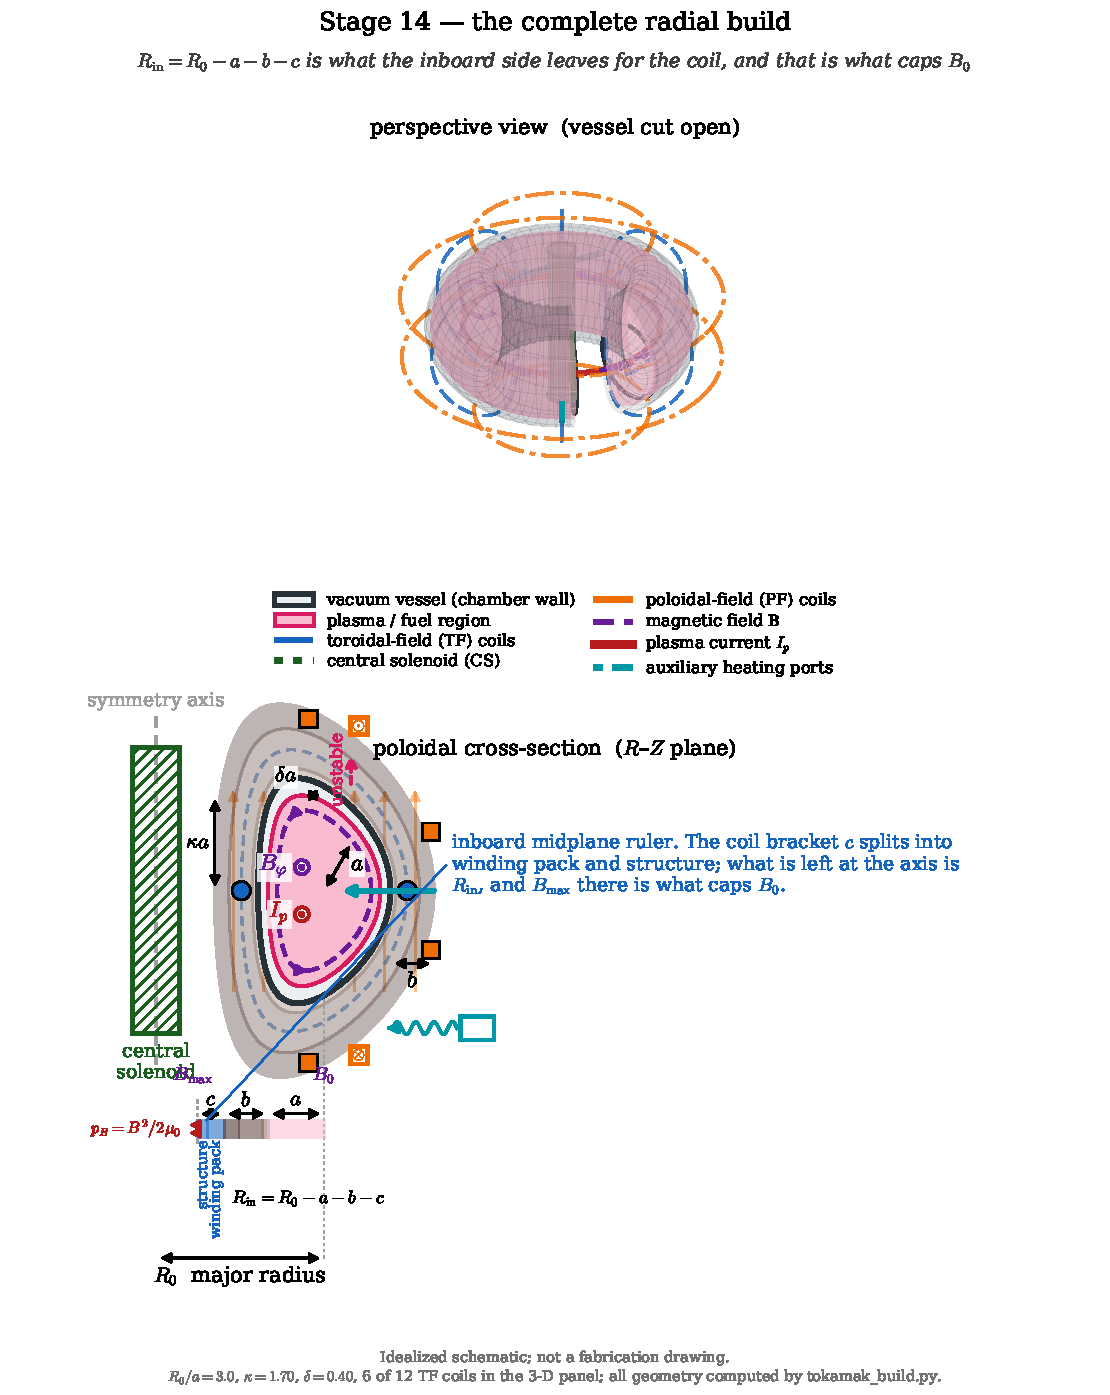
\includegraphics[width=1.0\textwidth]{figures/final/figM14_stage14_tall.pdf}
  \caption{Machine state: the complete radial build. $R_{\rm in}=R_0-a-b-c$ is what the inboard side leaves for the coil, and that is what caps $B_0$.}
  \label{fig:figM14_stage14_tall}
\end{figure}


% ============================= PAGE 49 ==============================
\newpage
\section*{49. The high-field door is now visible, but not yet opened}

We can now say precisely what a higher-field magnet changes. At fixed radial geometry,
Eq.~\eqref{eq:b0radialbuild} makes a higher allowable $B_{\max}$ available as a higher
central field $B_0$. But Eqs.~\eqref{eq:cstructure-scaling} and
\eqref{eq:winding-thickness} also show the price: field increases magnetic stress
quadratically and imposes a technology-dependent current-density requirement. "Use a
stronger magnet" is not a solution until both sides of this trade are analysed.

This is the correct logical location for high-temperature superconductors (HTS).
They are not needed to explain why a tokamak has TF coils, and they should not appear
as an unexplained early feature. They matter later if the baseline, conventional
field limit makes the plasma-current closure fail. At that point a conductor able to
operate at the required field and current density can raise $B_{\max}$; the rest of
the thesis must test whether the resulting improvement in current, stability, and
current drive outweighs the extra magnet build and cost.

\designconsequence{HTS is an enabling option for a specified high-field reactor
strategy, not a universal first-principles requirement for every conceivable tokamak.
The thesis will earn the stronger design claim only after the classical baseline has
been reconstructed and shown to require a field beyond its assumed conventional-magnet
limit.}

\supportingquantity{material field limit $B_{\max}$}{The maximum inboard coil field
is an engineering constraint rather than a Table-1 reactor parameter. It governs the
primary parameters $B_0$ and $c$ through the radial build. Later, a technology model
will compare a conventional superconducting limit with an HTS-enabled high-field
limit, including stress, protection, joints, neutron tolerance, and maintenance.}

\imagebrief{Reset trade-off sketch: field is performance and burden}{Create a
two-sided causal diagram, not a sales graphic. Left: higher $B_{\max}$ permits higher
$B_0$ at fixed radial build. Right: $p_B=B^2/(2\mu_0)$ raises structural demand and
can increase $c$. Add a dashed arrow labelled "test only after baseline closure" to
the later plasma-current/stability analysis. Do not yet draw an HTS brand, a
spherical tokamak, or a numerical performance claim.}

\begin{figure}[htbp]\centering
  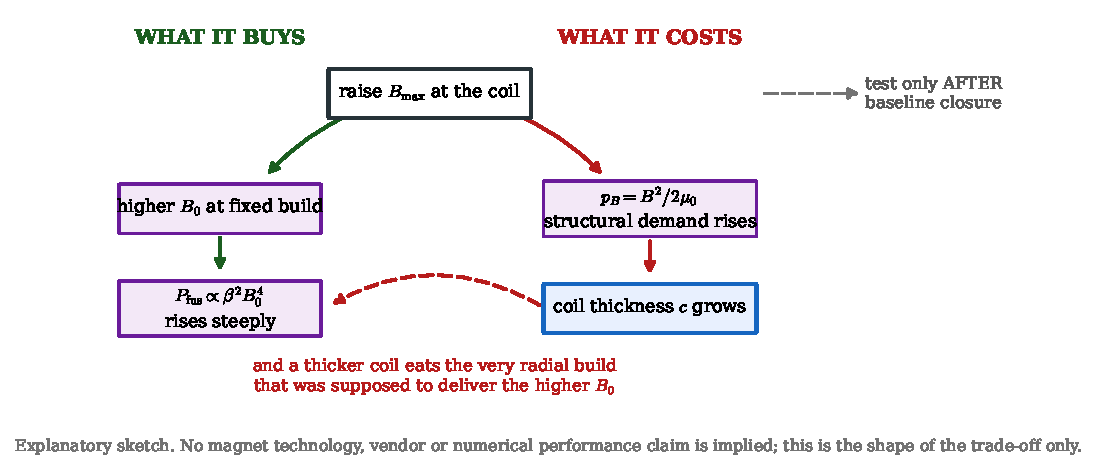
\includegraphics[width=1.0\textwidth]{figures/final/figS_field_two_sided.pdf}
  \caption{Reset trade-off sketch: field is performance and burden. \schematicnote}
  \label{fig:figS_field_two_sided}
\end{figure}


% ============================= PAGE 50 ==============================
\newpage
\section*{50. The primary design vocabulary is complete}

The tokamak has now revealed every member of the primary parameter set:
\[
 \boxed{a,\ R_0,\ \kappa,\ b,\ c,\ T,\ n,\ p,\ \tau_E,\ B_0,\ \beta,\ I,\ q_*,\ f_B.}
\]
They do not have the same logical status. Some describe geometry; some are plasma
state variables; some record magnetic/current balance; and $b,c$ are radial builds
forced by nuclear transport and magnet engineering. Nor are they independent. For
example, the causal relations already derived include
\[
 p=2nT,\qquad
 q_*\propto\frac{a^2B_0}{R_0I},\qquad
 B_0=B_{\max}\left(1-\frac{a+b+c}{R_0}\right).
\]
The purpose of writing them together is not to solve the reactor yet. It is to make
clear that a proposed change in one component propagates through the whole machine.

The next part of the thesis can therefore enter Freidberg's 2015 argument on honest
terms. It will select explicit engineering and nuclear assumptions, express the
primary parameters as coupled functions rather than isolated knobs, and then compare
the demanded plasma state with four operational tests: Greenwald density, Troyon beta,
kink safety factor, and achievable bootstrap fraction. The core question will be
whether all four inequalities can hold simultaneously for a conventional baseline.

\designconsequence{Only now is it legitimate to begin the numerical closure. If the
baseline fails, the later high-field/HTS discussion will be an earned response to a
specific contradiction, not an imported preference.}

\model{The open manuscript by J.~P.~Freidberg, F.~J.~Mangiarotti, and
J.~Minervini (2015), especially its Sections~3--6, is used here as a freely available
reference design. Its one-dimensional blanket and analytic TF-coil models motivate
the present derivation; the thesis will state their assumptions before reproducing any
numerical result.}

% ============================= PAGE 51 ==============================
\newpage
\section*{51. Entering the 2015 argument: a model, not a verdict}

We now change tasks. The first fifty pages asked, "Why must the machine contain these
parts?" The next task is, "If a particular conventional-reactor model is required to
make a specified amount of power, what plasma state does that model demand?" This is
the calculation made analytically by Freidberg, Mangiarotti, and Minervini in 2015.

Their reference design is intentionally simplified. It specifies an electric output,
an allowed neutron wall loading, a thermal conversion efficiency, a maximum inboard
coil field, magnet stress and winding-pack limits, and a cap on recirculating power.
It then asks whether a conventional plasma can simultaneously meet the resulting
density, beta, kink-safety-factor, and bootstrap-current requirements.

\designconsequence{The following conclusion, if reproduced, will be conditional:
there is no self-consistent reactor within the stated baseline assumptions. It will not
say that no tokamak can ever work. That distinction is where honest engineering begins.}

\model{Every numerical input in this reconstruction will be visibly tagged as either
an economic choice, an engineering limit, a nuclear-data/model choice, or an empirical
plasma-physics fit. Changing one of them defines a different reactor case; it is not a
mathematical error.}

% ============================= PAGE 52 ==============================
\newpage
\section*{52. The reference design asks the machine to do a specific job}

For the 2015 baseline, the primary imposed mission choices are
\[
 P_E=1000\,\mathrm{MW_e},\qquad
 W_n=4\,\mathrm{MW\,m^{-2}},\qquad
 \eta_T=0.40.
\]
$P_E$ is desired electric output, $W_n$ is the chosen upper bound on average neutron
wall loading, and $\eta_T$ converts fusion heat into electric power:
\begin{equation}
 P_E=\eta_TP_F.
 \label{eq:thermal-conversion}
\end{equation}
The subscript $F$ denotes the total thermal power credited to fusion and blanket
reactions in the paper's accounting model. The point of displaying these numbers is
not to bless them. A $1000\,\mathrm{MW_e}$ plant, a $4\,\mathrm{MW\,m^{-2}}$ wall
limit, and $40\%$ conversion efficiency are assumptions to be audited.

The reference magnet model also takes
\[
 B_{\max}=13\,\mathrm T,\qquad
 \sigma_{\rm allow}=600\,\mathrm{MPa},\qquad
 J_{\rm wp}=20\,\mathrm{MA\,m^{-2}}.
\]
These are a baseline conventional-superconductor and structural model, not claims
about the best magnets available today. They are precisely the assumptions later
challenged by the high-field option.

\supportingquantity{reference inputs}{The quantities $P_E,W_n,\eta_T,B_{\max},
\sigma_{\rm allow}$, and $J_{\rm wp}$ are inputs to a chosen design case. They guide
the determination of the primary parameter set; they are not additional Table-1
parameters.}

% ============================= PAGE 53 ==============================
\newpage
\section*{53. Power and wall loading turn two dimensions into one family}

For the shaped boundary, the source uses the standard mean-square ellipse-perimeter
approximation. Revolving it around the major radius gives the first-wall area
\begin{equation}
 S_{\rm wall}\simeq4\pi^2R_0a
 \left(\frac{1+\kappa^2}{2}\right)^{1/2}.
 \label{eq:shaped-wall-area}
\end{equation}
This agrees with the circular result $4\pi^2R_0a$ when $\kappa=1$. It is an
analytic shape approximation, not a replacement for an actual first-wall surface.

The D--T neutron carries $E_n=14.1\,\mathrm{MeV}$ of the fusion energy
$E_{\rm DT}=17.6\,\mathrm{MeV}$. In the reference energy accounting,
\[
 P_n=\frac{E_n}{E_F}P_F
 =\frac{E_n}{E_F}\frac{P_E}{\eta_T}.
\]
Equating neutron power to the allowed wall loading times the wall area,
$P_n=W_nS_{\rm wall}$, gives
\begin{equation}
 R_0a=
 \frac{E_nP_E}
 {4\pi^2E_FW_n\eta_T}
 \left(\frac{2}{1+\kappa^2}\right)^{1/2}.
 \label{eq:r0a-wall-loading}
\end{equation}
All quantities on the right are chosen inputs or previously earned parameters.
Thus the design does not choose $R_0$ and $a$ independently:
\begin{equation}
 R_0(a)=\frac{C_{\rm wall}}{a},
 \qquad
 C_{\rm wall}\equiv
 \frac{E_nP_E}{4\pi^2E_FW_n\eta_T}
 \left(\frac{2}{1+\kappa^2}\right)^{1/2}.
 \label{eq:r0-of-a}
\end{equation}
This is why Freidberg can make a one-parameter scan. After fixing the mission and
the blanket/magnet model, each trial minor radius implies a corresponding major radius.

\model{Equation~\eqref{eq:shaped-wall-area} uses a simple perimeter approximation and
an average wall loading. A final reactor analysis needs local neutron transport and
the actual first-wall surface. The one-parameter logic survives those refinements.}

% ============================= PAGE 54 ==============================
\newpage
\section*{54. The radial build makes the field a coupled result}

The preceding page makes $R_0$ a function of $a$. For its particular analytic
TF-coil calculation, Freidberg defines the inboard field-build fraction
\[
 \epsilon_B=\frac{a+b}{R_0}
\]
and writes
\[
 B_0=B_{\max}(1-\epsilon_B).
\]
This is the source model's field convention: $c$ is then found from its stress and
winding-pack equations, rather than inserted into $\epsilon_B$. The physical radial
ledger on pages 46--48 remains useful for understanding why $c$ exists; reproducing
the source's numerical scan requires us not to mix that fuller ledger with its
analytic convention. Its logical structure is more important than its algebra:
\[
\begin{array}{c}
\text{mission and wall loading}\ \Longrightarrow\ R_0(a),\\[2pt]
\text{neutron transport}\ \Longrightarrow\ b,\\[2pt]
\text{field, stress, and ampere-turns}\ \Longrightarrow\ c(a,B_0),\\[2pt]
\text{inboard radial build}\ \Longrightarrow\ B_0(a).
\end{array}
\]
The central field is therefore neither a free wish nor merely a property of the
superconductor. It is the outcome of a coupled geometric and mechanical problem.

This is also the first place to be alert to a future HTS comparison. If a different
conductor technology changes the credible $B_{\max}$ or $J_{\rm wp}$, it changes the
solution for $c$ and therefore the accessible $B_0$. We will not assume that this
improves the reactor until the baseline plasma constraints have been tested.

\imagebrief{Causal ledger diagram: how the reference design reduces to a scan in $a$}
{Make a compact flow diagram of the four arrows displayed above. Use a distinct style
for chosen inputs, primary parameters, and derived supporting quantities. End at
"test plasma constraints," not at a success claim. This is a reset explanatory figure,
not a cumulative machine image.}

\begin{figure}[htbp]\centering
  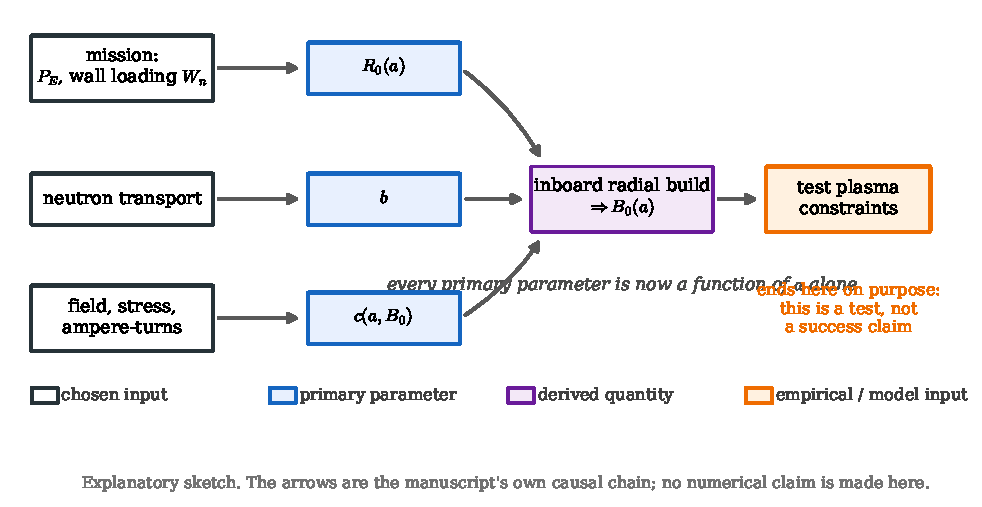
\includegraphics[width=1.0\textwidth]{figures/final/figS_causal_scan_in_a.pdf}
  \caption{Causal ledger diagram: how the reference design reduces to a scan in $a$. \schematicnote}
  \label{fig:figS_causal_scan_in_a}
\end{figure}


% ============================= PAGE 55 ==============================
\newpage
\section*{55. Fusion power fixes the required pressure}

The D--T reaction rate in an equal fuel mixture is
\[
 \mathcal R=\frac{n^2}{4}\langle\sigma v\rangle(T),
\]
because $n_D=n_T=n/2$. Multiplying by the energy released per reaction and integrating
over plasma volume gives
\begin{equation}
 P_{\rm fus}=
 \frac{\langle\sigma v\rangle(T)E_{\rm DT}}{4}
 \int n^2\,dV.
 \label{eq:baseline-fusion-power}
\end{equation}
For a first transparent estimate, use volume-averaged $n$ and $T$:
\[
 P_{\rm fus}\simeq
 \frac{\langle\sigma v\rangle(T)E_{\rm DT}}{4}\,n^2V.
\]
The equal-temperature quasineutral model gave $p=2nT$, hence
\begin{equation}
 P_{\rm fus}\simeq
 \frac{\langle\sigma v\rangle(T)E_{\rm DT}}{16T^2}\,p^2V.
 \label{eq:baseline-power-pressure}
\end{equation}
Power balance therefore determines a required pressure:
\begin{equation}
 p_{\rm req}\simeq
 \left[
 \frac{16T^2P_{\rm fus,req}}
 {\langle\sigma v\rangle(T)E_{\rm DT}V}
 \right]^{1/2}.
 \label{eq:preq}
\end{equation}
This is a crucial conceptual reversal. The plasma physicist does not simply choose a
pleasantly low pressure; the requested electric output and available volume demand one.

The 2015 reference model selects $T\simeq14\,\mathrm{keV}$ because the ratio
$\langle\sigma v\rangle/T^2$ is near its favorable broad maximum for D--T fuel. Later
we will reproduce that statement from a cited reactivity fit and replace the uniform
approximation with the paper's declared density and temperature profiles.

% ============================= PAGE 56 ==============================
\newpage
\section*{56. Ignition turns pressure into a required confinement time}

Fusion power does not remain as useful plasma heat. The neutron escapes; for D--T,
the alpha fraction is
\[
 \frac{E_\alpha}{E_{\rm DT}}=\frac{3.5}{17.6}\simeq\frac15.
\]
For an ignited plasma, alpha heating must replace the energy conducted and transported
out of the core. Let $W$ be thermal energy stored in the plasma and define
\[
 \tau_E=\frac{W}{P_{\rm loss}}.
\]
The ignition balance is $P_\alpha=P_{\rm loss}=W/\tau_E$, or
\begin{equation}
 \tau_{E,\rm req}=\frac{W}{P_\alpha}.
 \label{eq:taue-required}
\end{equation}

In the equal-temperature model, the thermal energy density is
$w=\tfrac32(n_e+n_i)T=3nT=\tfrac32p$. Thus $W\simeq\tfrac32pV$. With
$P_\alpha\simeq P_{\rm fus}/5$,
\begin{equation}
 \tau_{E,\rm req}\simeq
 \frac{15pV}{2P_{\rm fus}}.
 \label{eq:taue-pressure}
\end{equation}
Substituting the pressure demanded by Eq.~\eqref{eq:preq} gives the next causal
chain:
\[
 P_E,\ W_n,\ \eta_T,\ a
 \ \Longrightarrow\ R_0,\ V,\ p
 \ \Longrightarrow\ \tau_{E,\rm req}.
\]
The remaining, decisive question is whether an empirical tokamak confinement law can
deliver this $\tau_E$ without demanding an unacceptable plasma current. That is where
the one indispensable plasma-physics input enters the 2015 design.

% ============================= PAGE 57 ==============================
\newpage
\section*{57. Before testing a limit: what kind of statement is it?}

The four tests ahead do not all have the same epistemic status. It would be a serious
error to place them in one box labelled "first principles." We will use three labels.

\begin{center}
\begin{tabular}{p{0.22\textwidth}p{0.66\textwidth}}
\textbf{Derived relation} & follows from stated equations and stated approximations;
for example, $p=2nT$ and $q_*\propto a^2B_0/(R_0I)$.\\[3pt]
\textbf{Physics model} & follows after adopting a specified equilibrium, profile, or
kinetic model; it may be calculated but is not universal.\\[3pt]
\textbf{Empirical boundary} & summarizes experimental operation or a regression; its
coefficient and range are evidence, not a theorem.
\end{tabular}
\end{center}

Greenwald density is an empirical boundary. The practical Troyon beta coefficient is
an experiment- and model-informed stability boundary. The kink threshold is a result
of a specified MHD stability model, with profile and wall dependence. The bootstrap
fraction requires a neoclassical kinetic model plus a current profile. Their physical
motivation can be derived; their reactor-grade numerical coefficients cannot honestly
be manufactured from the motivation alone.

The test itself is nevertheless elementary. For every constraint define a demand-to-
allowance ratio,
\begin{equation}
 \mathcal R\equiv\frac{\hbox{quantity demanded by the reference design}}
 {\hbox{quantity allowed by the stated constraint}}.
 \label{eq:constraint-ratio}
\end{equation}
A baseline is admissible only if each relevant $\mathcal R\le1$. This notation forces
us to name both numerator and denominator before announcing pass or failure.

\designconsequence{The goal is not to make empirical plasma physics look more certain
than it is. The goal is to expose exactly which evidence a conventional reactor would
need to satisfy, and whether the same design point can satisfy all of it at once.}

% ============================= PAGE 58 ==============================
\newpage
\section*{58. The one empirical input that determines the required current}

The 2015 reference case uses an ELMy H-mode confinement regression. H-mode is a
high-confinement tokamak regime with a strong edge transport barrier. ELMy means that
the edge undergoes recurring edge-localized-mode (ELM) relaxations: short bursts that
expel a small amount of edge energy and particles. The word identifies the experiment
class behind the regression; it does not add an independently derived law.\footnote{A
freely accessible ITER explanation describes H-mode's steep edge pressure region and
the associated edge-localized modes: \url{https://www.iter.org/node/20687/progress-elm-physics-and-elm-control}.}
In the declared units, the regression is
\begin{equation}
\tau_E =
0.145H\,
\frac{I^{0.93}R_0^{1.39}a^{0.58}\kappa^{0.78}
\bar n^{0.41}B_0^{0.15}A^{0.19}}
{P_\alpha^{0.69}}
\quad\mathrm{s}.
\label{eq:freidberg-confinement}
\end{equation}
Here $I$ is in MA, $R_0$ and $a$ in m, $\bar n$ in
$10^{20}\,\mathrm{m^{-3}}$, $B_0$ in T, $P_\alpha$ in MW, $A=2.5$ is the
mean ion mass used by the fit, and $H$ is the confinement multiplier. The coefficient
is meaningless if these units or the database/regime are changed.

Equation~\eqref{eq:freidberg-confinement} is not deduced from the Lorentz force. It
is the particular empirical closure selected by the paper. Its physical direction is
intelligible: larger current and machine size correlate with better confinement;
greater heating power correlates with more difficult power exhaust. But the exponents
are measured regression exponents, not universal laws of nature.

\supportingquantity{reference confinement fit}{Equation~\eqref{eq:freidberg-confinement}
is the explicit version of $\tau_E=H\tau_{E,\rm ref}$ used in this reconstruction.
It is the one direct plasma-performance input that turns the ignition requirement
into a required current. The freely available source is Freidberg, Mangiarotti, and
Minervini (2015), Eq.~(28), linked on page 1 of this thesis.}

\model{The reference paper assumes $H=1$ for its conventional baseline. We will retain
that assumption only while reproducing that baseline, then vary it openly when testing
the advanced-confinement option.}

% ============================= PAGE 59 ==============================
\newpage
\section*{59. Solving the confinement fit for the current}

The ignition calculation has already supplied $\tau_{E,\rm req}$. Set it equal to the
right side of Eq.~\eqref{eq:freidberg-confinement} and isolate the only unknown in
this step, $I$:
\[
 I^{0.93}=
\frac{\tau_{E,\rm req}P_\alpha^{0.69}}
{0.145H R_0^{1.39}a^{0.58}\kappa^{0.78}
\bar n^{0.41}B_0^{0.15}A^{0.19}}.
\]
Raising both sides to the power $1/0.93$ gives
\begin{equation}
 I_{\rm req}=
\left[
\frac{\tau_{E,\rm req}P_\alpha^{0.69}}
{0.145H R_0^{1.39}a^{0.58}\kappa^{0.78}
\bar n^{0.41}B_0^{0.15}A^{0.19}}
\right]^{1/0.93}\mathrm{MA}.
\label{eq:ireq-from-confinement}
\end{equation}
There is no mystery step here: the current is whatever value makes the selected
empirical confinement law equal the confinement time required by ignition.

After substituting the reference design's previously determined relations, Freidberg
obtains the compact scaling
\begin{equation}
 I_{\rm req}\simeq
 12.1\,\frac{a^{1.63}}{B_0^{0.16}}\ \mathrm{MA},
\label{eq:ireq-compact}
\end{equation}
where the remaining fixed baseline assumptions and the stated units are absorbed into
the coefficient. The striking feature is not the exact decimal exponents. It is the
strong approximately $a^{5/3}$ current demand and the weak $B_0^{-0.16}$ dependence.

For the reference point $a=1.34\,\mathrm m$ and $B_0=6.83\,\mathrm T$, the paper
finds $I_{\rm req}=14.3\,\mathrm{MA}$. This is a demanded current, not a performance
target selected because it is easy to sustain.

\imagebrief{Reset derivation sketch: confinement requirement becomes current demand}
{Show a left-to-right chain: ignition power balance gives $\tau_{E,\rm req}$; the
explicit empirical fit gives $\tau_E(I)$; equating them produces $I_{\rm req}$. Put
the words "fit, not theorem" directly beneath the confinement-law block. Include the
weak $B_0^{-0.16}$ and strong $a^{1.63}$ reference scaling.}

\begin{figure}[htbp]\centering
  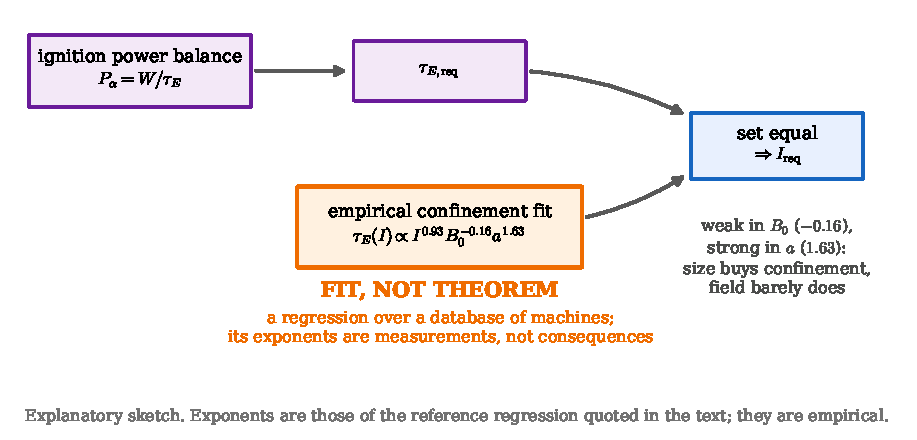
\includegraphics[width=1.0\textwidth]{figures/final/figS_confinement_to_current.pdf}
  \caption{Reset derivation sketch: confinement requirement becomes current demand. \schematicnote}
  \label{fig:figS_confinement_to_current}
\end{figure}


% ============================= PAGE 60 ==============================
\newpage
\section*{60. High required current immediately tests field-line twist}

The safety factor was introduced as the number of toroidal circuits made by a field
line per poloidal circuit. At the plasma edge, more plasma current produces more
poloidal field, so it reduces this twist count. For the elongated reference geometry,
the paper uses
\begin{equation}
 q_*=
\frac{2\pi a^2B_0}{\mu_0R_0I}
\left(\frac{1+\kappa^2}{2}\right).
\label{eq:freidberg-qstar}
\end{equation}
The first factor is the Amp\`ere-law estimate already derived from
$B_\theta\sim\mu_0I/(2\pi a)$; the shape factor records the paper's chosen elongation
correction. Thus substituting $I_{\rm req}$, not an independently chosen current,
produces the required $q_*$.

Why does a lower $q_*$ matter? A current-carrying plasma column contains free energy.
A helical displacement can bend and reconnect the field in a way that releases some
of that current-associated magnetic energy. The exact stability boundary depends on
current profile, pressure profile, wall response, rotation, and mode number. The
reference model uses the practical external-kink/disruption condition
\begin{equation}
 q_*\ge q_K,\qquad q_K\simeq2.
\label{eq:kink-boundary}
\end{equation}
Here a disruption means an abrupt loss of controlled plasma equilibrium and
confinement, commonly accompanied by a rapid current termination and large transient
loads. The mechanism is MHD current-driven instability; the numerical threshold is a
stated model boundary, not a number obtained by setting two elementary equations
equal.

\supportingquantity{kink ratio}{The transparent test is
$\mathcal R_K=q_K/q_*$. It is below one only when the demanded current leaves enough
field-line twist to meet the adopted kink-safety criterion.}

% ============================= PAGE 61 ==============================
\newpage
\section*{61. The four tests are now motivated, not imported}

At the same reference design point, evaluate four distinct ratios:
\begin{align}
 \mathcal R_G&=\frac{n}{n_G},
 &n_G&=\frac{I}{\pi a^2}\times10^{20}\,\mathrm{m^{-3}},
 \label{eq:ratio-greenwald}\\
 \mathcal R_T&=\frac{\beta}{\beta_T},
 &\beta_T&=\beta_N\frac{I}{aB_0},
 \label{eq:ratio-troyon}\\
 \mathcal R_K&=\frac{q_K}{q_*},
 &q_K&\simeq2,
 \label{eq:ratio-kink}\\
 \mathcal R_B&=\frac{f_B}{f_{\rm NC}}.
 &&
 \label{eq:ratio-bootstrap}
\end{align}
Units in the Greenwald and normalized-beta forms are the conventional MA--m--T units
stated earlier. Each ratio has a different physical origin:

\begin{itemize}
\item $\mathcal R_G$ checks the experimentally observed density boundary introduced
on page 35;
\item $\mathcal R_T$ checks pressure against the practical MHD beta allowance
motivated on pages 33--34;
\item $\mathcal R_K$ checks the current-driven kink boundary just explained;
\item $\mathcal R_B$ checks whether non-inductive current sources can replace the
required current in steady state.
\end{itemize}

The notation makes the decision rule uniform but does not erase the different kinds
of evidence behind the four denominators. A claim that the reactor "passes plasma
physics" will be permitted only after every one of these ratios is shown, with its
assumptions, at the same design point.

\designconsequence{The current required by confinement appears in every test: directly
in $n_G$, $\beta_T$, and $q_*$, and indirectly in the current balance. This is why
the conventional-tokamak difficulty has a common root rather than four unrelated
problems.}

% ============================= PAGE 62 ==============================
\newpage
\section*{62. First audit: the density requirement}

The fusion-power calculation demands the reference average density
\[
 n=1.43\times10^{20}\,\mathrm{m^{-3}}.
\]
The Greenwald reference density, using the confinement-demanded
$I=14.3\,\mathrm{MA}$ and $a=1.34\,\mathrm m$, is
\[
 n_G=
\frac{14.3}{\pi(1.34)^2}\times10^{20}\,\mathrm{m^{-3}}
=2.54\times10^{20}\,\mathrm{m^{-3}}.
\]
Therefore
\begin{equation}
 \mathcal R_G=\frac{1.43}{2.54}=0.56<1.
\label{eq:greenwald-reference}
\end{equation}
The baseline passes this particular test with margin. That result is valuable: it
shows the later failure is not created by declaring every well-known limit violated.

\model{The use of the Greenwald relation at reactor scale remains an extrapolation.
The conclusion here is only that the 2015 baseline lies below the boundary assumed by
that model. It is not a first-principles proof that such a density is attainable in a
burning reactor.}

% ============================= PAGE 63 ==============================
\newpage
\section*{63. Second audit: pressure is barely allowed}

The same reference design requires
\[
 \beta=4.13\%.
\]
Its adopted normalized-beta coefficient is $\beta_N=2.8$. With
$I=14.3\,\mathrm{MA}$, $a=1.34\,\mathrm m$, and $B_0=6.83\,\mathrm T$,
\[
 \beta_T=
 2.8\,\frac{14.3}{(1.34)(6.83)}\%=4.39\%.
\]
Thus
\begin{equation}
 \mathcal R_T=\frac{4.13}{4.39}=0.94<1.
\label{eq:troyon-reference}
\end{equation}
The comparison passes, but only narrowly. It is not a reserve that can be spent
silently on profile changes, control margin, or modelling error.

\model{The $2.8$ coefficient is the reference model's Troyon-normalized-beta
assumption. A different equilibrium, wall, profile, or stability-control model can
change it. The algebra above is exact once that assumption and its conventional units
are stated; the coefficient itself is not derived from the algebra.}

% ============================= PAGE 64 ==============================
\newpage
\section*{64. Third audit: the confinement-driven current fails the kink test}

Insert the same demanded current into Eq.~\eqref{eq:freidberg-qstar}. The reference
calculation gives
\[
 q_*=1.56.
\]
The adopted disruption-avoidance threshold is $q_K\simeq2$, so
\begin{equation}
 \mathcal R_K=\frac{2}{1.56}=1.28>1.
\label{eq:kink-reference}
\end{equation}
This is a failure of the stated baseline. The required current produces insufficient
edge field-line twist for the adopted kink-safety margin.

Notice the causal chain. The kink problem was not inserted after the reactor was
chosen. Electric output and wall loading demanded pressure and volume; ignition
demanded $\tau_E$; the confinement fit demanded $I$; that $I$ forced $q_*$ below the
adopted stability boundary. Reducing current would improve $q_*$, but would then fail
to provide the empirical confinement time used in the baseline.

\imagebrief{Causal failure sketch: why the kink ratio exceeds one}{Draw the chain
$P_E,W_n\rightarrow p,V\rightarrow\tau_{E,\rm req}\rightarrow I_{\rm req}
\rightarrow q_*\rightarrow\mathcal R_K$. Mark the last comparison
$1.28>1$ as a reference-model failure. Include a note that $q_K\simeq2$ is a
profile/wall-dependent stability-model input.}

\begin{figure}[htbp]\centering
  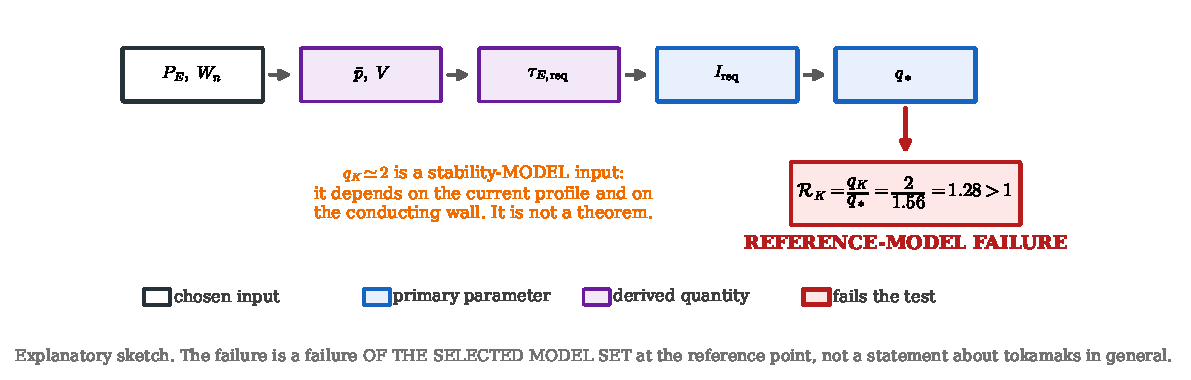
\includegraphics[width=1.0\textwidth]{figures/final/figS_kink_failure_chain.pdf}
  \caption{Causal failure sketch: why the kink ratio exceeds one. \schematicnote}
  \label{fig:figS_kink_failure_chain}
\end{figure}


% ============================= PAGE 65 ==============================
\newpage
\section*{65. Fourth audit begins with a current ledger, not a magic bootstrap number}

A steady-state tokamak cannot rely on a transformer indefinitely. Its current ledger
must be
\[
 I=I_{\rm CD}+I_{\rm bs},
\]
where $I_{\rm CD}$ is externally driven current and $I_{\rm bs}$ is bootstrap current.
Divide by the required total current:
\begin{equation}
 1=\frac{I_{\rm CD}}{I}+f_B,
 \qquad
 f_B=1-\frac{I_{\rm CD}}{I}.
\label{eq:required-bootstrap}
\end{equation}
This equation is only charge accounting. It does not claim that the plasma can supply
the required $f_B$.

For the reference recirculating-power and lower-hybrid current-drive model, the paper
obtains $I_{\rm CD}=2.25\,\mathrm{MA}$. With $I=14.3\,\mathrm{MA}$,
\begin{equation}
 f_B=1-\frac{2.25}{14.3}=0.84.
\label{eq:required-bootstrap-reference}
\end{equation}
The required bootstrap fraction is therefore very large because the demanded current
is large while economically permitted external drive is limited.

The next task is not to announce a bootstrap limit from nowhere. We must derive the
physical source of bootstrap current from trapped-particle collisional asymmetry, state
the selected neoclassical current-density model, and integrate it over the declared
profiles to obtain the achievable fraction $f_{\rm NC}$. Only then can we evaluate
$\mathcal R_B=f_B/f_{\rm NC}$.

\designconsequence{Three audited comparisons now exist: density passes, beta is
marginal, and kink safety fails. The remaining steady-state test will ask whether the
pressure gradients that help make fusion power can naturally supply enough current to
replace what the transformer cannot.}

% ============================= PAGE 66 ==============================
\newpage
\section*{66. Where bootstrap current actually comes from}

Page 36 established the first ingredient: a torus has trapped as well as passing
particles. Page 37 stated the second: the pressure falls from the hot, dense core
toward the edge. Put those facts together, but do not yet call the result a formula.

In a uniform straight field, particles moving parallel to $\mathbf B$ in the two
directions can cancel one another's current. In a torus, trapped particles bounce
between mirror points and do not complete a full parallel circuit. A pressure gradient
means that the population arriving from the core side of a narrow radial shell is not
identical to the population arriving from the edge side. Grad-$B$ and curvature drifts
then separate the two populations slightly. Collisions transfer part of that imbalance
between trapped and passing particles. The cancellation of parallel electron motion is
therefore incomplete: a toroidal current remains.

The energy source is not mysterious. It is the pressure profile itself. Flatten the
profile so that $dp/dr=0$, and the drive disappears. Make the profile steeper, and the
available drive grows, while the pressure-gradient stability burden grows with it.
This is precisely why bootstrap current belongs in the same closure problem as beta
and kink safety.

\imagebrief{Physics sketch: from trapped particles to bootstrap current}{Draw a
small annular plasma shell. On the inboard side show stronger field and trapped
electron bounce points; on the outboard side show passing electrons. Add an outward
pressure-gradient arrow and a collision arrow transferring the trapped-particle
asymmetry to passing electrons. End with a modest toroidal-current arrow labelled
``incomplete cancellation,'' not ``free current.''}

\begin{figure}[htbp]\centering
  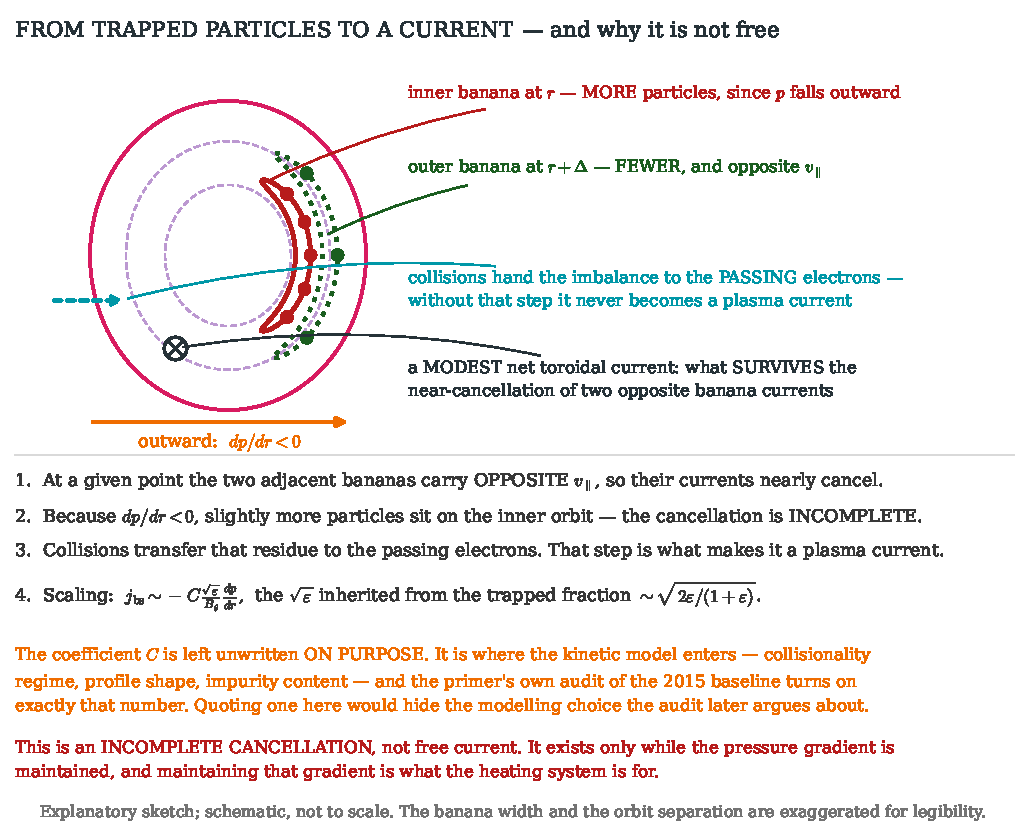
\includegraphics[width=1.0\textwidth]{figures/final/figS_bootstrap_from_trapped.pdf}
  \caption{Physics sketch: from trapped particles to bootstrap current. \schematicnote}
  \label{fig:figS_bootstrap_from_trapped}
\end{figure}


\designconsequence{The pressure gradient that is required to make fusion power also
creates a possible self-current. Whether it is large enough is not an independent
choice: it must be calculated from a kinetic model, the same profiles, and the
magnetic geometry already demanded by the reactor.}

% ============================= PAGE 67 ==============================
\newpage
\section*{67. The first irreducibly kinetic input is declared, not smuggled in}

The mathematical object behind the preceding paragraph is a drift-kinetic equation.
In schematic form for a distribution function $f(\mathbf x,\mathbf v)$ it is
\begin{equation}
 \left(v_\parallel\mathbf b+\mathbf v_d\right)\!\cdot\!\nabla f
 +\frac{qE_\parallel}{m}\frac{\partial f}{\partial v_\parallel}
 =C[f].
 \label{eq:drift-kinetic-schematic}
\end{equation}
Here $\mathbf b=\mathbf B/B$, $\mathbf v_d$ represents the guiding-center drifts,
and $C[f]$ is the Coulomb collision operator. Solving Eq.~\eqref{eq:drift-kinetic-schematic}
with trapped orbits is beyond a first course in differential equations; writing a
number for it without acknowledgement would be worse than leaving a difficult step
visible.

Freidberg, Mangiarotti, and Minervini therefore choose a particular large-aspect-ratio,
low-collisionality neoclassical closure. They assume equal ion and electron
temperatures, $T_i=T_e=T$, one effective ion charge, $Z=1$, and a circular
area-equivalent radius
\begin{equation}
 \hat a=\kappa^{1/2}a,\qquad \rho=\frac r{\hat a}.
 \label{eq:ahat-rho}
\end{equation}
Their local bootstrap-current model is their Eq.~(41):
\begin{equation}
 J_B(\rho)=-2.44\left(\frac r{R_0}\right)^{1/2}\frac p{B_\theta}
 \left(\frac1n\frac{dn}{dr}+0.055\,\frac1T\frac{dT}{dr}\right).
 \label{eq:freidberg-local-bootstrap}
\end{equation}
The coefficient $2.44$ and the relative temperature-gradient weight $0.055$ are the
kinetic closure, expressed in the paper's conventional working units; they are not
deducible from Maxwell's equations and elementary calculus alone. Everything from
this point onward---the gradients, the poloidal field, the area integral, and the
comparison with the required fraction---can and will be shown explicitly.

\model{Equation~\eqref{eq:freidberg-local-bootstrap} is a declared neoclassical
model, not a universal bootstrap law. Its regime assumptions, effective charge,
collisionality treatment, and chosen profiles are part of the result. The accessible
source is Freidberg, Mangiarotti, and Minervini (2015), Eq.~(41).}

% ============================= PAGE 68 ==============================
\newpage
\section*{68. The selected profiles make the pressure-gradient term calculable}

The same paper does not leave $n(r)$ and $T(r)$ implicit. Its standard-profile choice
(its Eq.~(20)) is
\begin{equation}
 T=2\bar T(1-\rho^2),\qquad
 p=2.5\bar p(1-\rho^2)^{3/2},\qquad
 n=1.5\bar n(1-\rho^2)^{1/2}.
 \label{eq:freidberg-profiles}
\end{equation}
The numerical factors make the bars cross-sectional averages. For example,
$\int_0^1 2\rho\,[2\bar T(1-\rho^2)]\,d\rho=\bar T$.

Because $d\rho/dr=1/\hat a$, ordinary differentiation gives
\begin{align}
 \frac1n\frac{dn}{dr}
 &=\frac{1}{1.5\bar n(1-\rho^2)^{1/2}}
 \left[1.5\bar n\,\frac12(1-\rho^2)^{-1/2}
       \left(-2\rho\right)\frac1{\hat a}\right]
 =-\frac{\rho}{\hat a(1-\rho^2)},\\
 \frac1T\frac{dT}{dr}
 &=\frac{1}{2\bar T(1-\rho^2)}
 \left[2\bar T\left(-2\rho\right)\frac1{\hat a}\right]
 =-\frac{2\rho}{\hat a(1-\rho^2)}.
 \label{eq:profile-log-gradients}
\end{align}
Thus the bracket in Eq.~\eqref{eq:freidberg-local-bootstrap} is
\begin{equation}
 \frac1n\frac{dn}{dr}+0.055\frac1T\frac{dT}{dr}
 =-\frac{(1+0.110)\rho}{\hat a(1-\rho^2)}.
 \label{eq:bootstrap-gradient-combination}
\end{equation}
Substitution of Eqs.~\eqref{eq:freidberg-profiles} and
\eqref{eq:bootstrap-gradient-combination} into Eq.~\eqref{eq:freidberg-local-bootstrap}
then gives, with $2.44(1.110)(2.5)=6.77\simeq6.8$,
\begin{equation}
 J_B(\rho)=6.8\,\frac{\bar p}{\hat a^{1/2}R_0^{1/2}}
 \frac{\rho^{3/2}(1-\rho^2)^{1/2}}{B_\theta(\rho)}.
 \label{eq:bootstrap-profiled-current}
\end{equation}
The sign convention is now carried by the direction chosen for $B_\theta$ and plasma
current. The useful content is transparent: this model predicts a current density
which vanishes at the axis and edge and is driven in the finite-gradient interior.

% ============================= PAGE 69 ==============================
\newpage
\section*{69. The poloidal field is obtained from the assumed total-current profile}

Equation~\eqref{eq:bootstrap-profiled-current} still contains $B_\theta(\rho)$.
It cannot be chosen after seeing the desired answer: it is produced by the total
plasma-current profile. The paper selects
\begin{equation}
 J_T(\rho)=\frac{I}{\pi\hat a^2}\frac{9\rho^{1/4}}8
 \frac{\alpha^2(1-x)e^{\alpha x}}{e^\alpha-1-\alpha},
 \qquad x=\rho^{9/4},\quad\alpha=2.53.
 \label{eq:freidberg-total-current-profile}
\end{equation}
This is another profile assumption, chosen to put appreciable current away from the
axis. It is normalized correctly: using $\rho=x^{4/9}$ gives
\begin{equation}
 \rho^{1/4}\rho\,d\rho=\frac49\,dx,
 \qquad
 \frac{I_{\rm enc}}I
 =\int_0^x\frac{\alpha^2(1-u)e^{\alpha u}}{e^\alpha-1-\alpha}\,du.
 \label{eq:enclosed-current-step}
\end{equation}
The antiderivative is
\begin{equation}
 \int\alpha^2(1-u)e^{\alpha u}\,du
 =\left(1+\alpha-\alpha u\right)e^{\alpha u},
 \label{eq:current-profile-antiderivative}
\end{equation}
so evaluation between $0$ and $x$ yields
\begin{equation}
 \frac{I_{\rm enc}}I=
 \frac{(1+\alpha-\alpha x)e^{\alpha x}-1-\alpha}{e^\alpha-1-\alpha}.
 \label{eq:enclosed-current}
\end{equation}
Ampere's law $2\pi rB_\theta=\mu_0I_{\rm enc}$ now gives
\begin{equation}
 b_\theta(\rho)\equiv\frac{B_\theta}{\mu_0I/(2\pi\hat a)}
 =\frac1\rho\left[
 \frac{(1+\alpha-\alpha x)e^{\alpha x}-1-\alpha}{e^\alpha-1-\alpha}
 \right].
 \label{eq:freidberg-btheta}
\end{equation}
This is the missing magnetic denominator in the bootstrap calculation. No additional
machine component has appeared; we have only made the previously required current
profile explicit.

% ============================= PAGE 70 ==============================
\newpage
\section*{70. Integrate the local current, then test the steady-state requirement}

In the area-equivalent circular cross-section, $dA=2\pi\hat a^2\rho\,d\rho$ after
integrating over the polar angle. Thus
\begin{align}
 I_B&=2\pi\hat a^2\int_0^1J_B(\rho)\rho\,d\rho\\
 &=2\pi\hat a^2\int_0^1
 \left[6.8\frac{\bar p}{\hat a^{1/2}R_0^{1/2}}
 \frac{\rho^{3/2}(1-\rho^2)^{1/2}}{B_\theta}\right]\rho\,d\rho.
 \label{eq:bootstrap-area-integral}
\end{align}
Replace $B_\theta$ using Eq.~\eqref{eq:freidberg-btheta}, divide by $I$, and collect
constants. Since $4\pi^2(6.8)=268.5$, the result is the paper's Eq.~(44):
\begin{equation}
 f_{\rm NC}\equiv\frac{I_B}{I}
 =268\frac{\hat a^{5/2}\bar p}{\mu_0R_0^{1/2}I^2}
 \int_0^1\frac{\rho^{5/2}(1-\rho^2)^{1/2}}{b_\theta(\rho)}\,d\rho.
 \label{eq:freidberg-bootstrap-fraction}
\end{equation}
This integral has no elementary antiderivative. That is not a gap in the argument: it
is a fully specified one-dimensional numerical quadrature. With $\alpha=2.53$, its
dimensionless value is $0.318$ (three significant figures). For the reference point,
\begin{equation}
 \kappa=1.70,\quad \hat a=\sqrt{1.70}(1.34\,\mathrm m)=1.747\,\mathrm m,
 \quad \bar p=7.57\,\mathrm{atm},\quad R_0=5.34\,\mathrm m,\quad
 I=14.3\,\mathrm{MA},
 \label{eq:bootstrap-reference-inputs}
\end{equation}
where $1\,\mathrm{atm}=101325\,\mathrm{Pa}$ and $1\,\mathrm{MA}=10^6\,\mathrm A$.
Equation~\eqref{eq:freidberg-bootstrap-fraction} then gives
\begin{equation}
 f_{\rm NC}=0.44.
 \label{eq:bootstrap-reference-result}
\end{equation}
The required value from Eq.~\eqref{eq:required-bootstrap-reference} was $f_B=0.84$.
The audited comparison is therefore
\begin{equation}
 \mathcal R_B=\frac{f_B}{f_{\rm NC}}=\frac{0.84}{0.44}=1.91>1.
 \label{eq:bootstrap-reference-ratio}
\end{equation}
This is a failure of the selected standard-profile neoclassical model: its calculated
self-current is about half the required self-current. It is not a proof that no
tokamak can ever operate steadily.

% ============================= PAGE 71 ==============================
\newpage
\section*{71. What the four tests have, and have not, established}

The baseline can now be read as one causal argument rather than a bag of named limits:
\begin{center}
\begin{tabular}{l c c l}
\textbf{Test} & \textbf{ratio} & \textbf{status} & \quad\textbf{meaning}\\
\hline
Greenwald density & $\mathcal R_G=0.56$ & passes & density is below the adopted empirical boundary\\
Troyon beta & $\mathcal R_T=0.94$ & marginal & pressure is near the adopted MHD boundary\\
Kink safety & $\mathcal R_K=1.28$ & fails & required current gives too little $q_*$ margin\\
Bootstrap closure & $\mathcal R_B=1.91$ & fails & calculated self-current is below required current share
\end{tabular}
\end{center}
The first two boundaries are empirical or model-dependent operating margins. The last
two failures are coupled: fusion mission and wall loading demand $p$ and volume;
ignition and the confinement fit demand $I$; that current lowers $q_*$, while the
same pressure profile can supply only a limited bootstrap share under the declared
kinetic model.

\imagebrief{Reset sketch: the conventional baseline's two coupled closure failures}{
Draw one concise logic map. Mission and wall loading lead to $p,V$; ignition and the
confinement fit lead to $I$. Split into two branches: $I\rightarrow q_*\rightarrow
\mathcal R_K=1.28>1$, and pressure profile plus trapped-particle kinetic model
$\rightarrow f_{\rm NC}=0.44$ compared with $f_B=0.84$, hence
$\mathcal R_B=1.91>1$. Keep density and beta as side checks marked pass and marginal.
Label every threshold or regression as model/empirical rather than first principle.}

\begin{figure}[htbp]\centering
  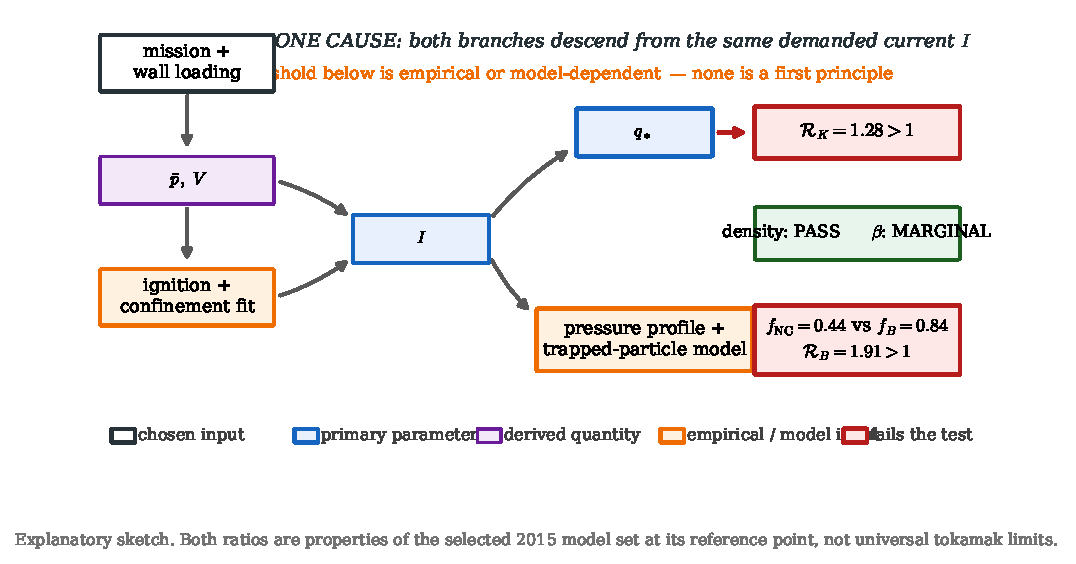
\includegraphics[width=1.0\textwidth]{figures/final/figS_two_closure_failures.pdf}
  \caption{Reset sketch: the conventional baseline's two coupled closure failures. \schematicnote}
  \label{fig:figS_two_closure_failures}
\end{figure}


\designconsequence{The conventional reference point is not rejected because a named
limit appeared from the left field. It fails two explicit closure tests after their
physical origin, profile assumptions, and calculation have been exposed. The next
question is which previously declared demands can be changed together without simply
moving the failure elsewhere.}

% ============================= PAGE 72 ==============================
\newpage
\section*{72. A reference point is not a design-space conclusion}

The reference point $a=1.34\,\mathrm m$ was chosen in the source by imposing
$R_0/a=4$. It is a useful check, but it cannot establish that the conventional
baseline fails at every size. The wall-loading calculation fixes instead
\begin{equation}
 R_0(a)=\frac{7.16}{a}\ \mathrm m
 \qquad (\kappa=1.70,\ \text{2015 baseline inputs}),
 \label{eq:freidberg-r0-scan}
\end{equation}
so $a$ is the remaining geometric trial variable.

For every trial $a$, the source's analytic radial-build convention supplies
\begin{equation}
 \epsilon_B(a)=\frac{a+b}{R_0(a)},\qquad
 B_0(a)=B_{\max}[1-\epsilon_B(a)],
 \quad b=1.20\,\mathrm m,\quad B_{\max}=13\,\mathrm T.
 \label{eq:freidberg-b0-scan}
\end{equation}
Its TF-coil stress and winding-pack model then determines $c(a)$; the plasma
calculation does not get to prescribe $c$ afterward. This is an important bookkeeping
point. The physical build developed earlier explains why the magnet has finite radial
thickness. Equation~\eqref{eq:freidberg-b0-scan} is the particular reduced
convention required to reproduce this paper's numerical scan.

The already-derived power and ignition relations become compact functions of $a$:
\begin{equation}
 \bar p(a)=\frac{8.76}{a^{1/2}}\ \mathrm{atm},\qquad
 \bar n(a)=\frac{1.66}{a^{1/2}}\times10^{20}\,\mathrm{m^{-3}},\qquad
 \tau_E(a)=0.81a^{1/2}\ \mathrm s.
 \label{eq:freidberg-state-scan}
\end{equation}
These are not new laws of nature. They are the stated mission, profile, and
wall-loading model expressed as a one-parameter family.

% ============================= PAGE 73 ==============================
\newpage
\section*{73. The current-drive allowance must move with the trial design}

In the reference case, $I_{\rm CD}=2.25\,\mathrm{MA}$ was obtained from a fixed
recirculating-power allowance. A scan must not hold that number fixed when density,
field, and size change. The power allocated to waves is
\begin{equation}
 P_{\rm CD}=\eta_{\rm RF}\eta_{\rm kly}f_{\rm RP}P_E
 =(0.80)(0.50)(0.10)P_E=40\,\mathrm{MW}.
 \label{eq:current-drive-power-scan}
\end{equation}
The source's lower-hybrid model writes the local efficiency in its conventional
units as
\begin{equation}
 \eta_{\rm CD}\equiv\frac{R_0\bar n I_{\rm CD}}{P_{\rm CD}}
 \simeq\frac{1.2}{n_\parallel^2}.
 \label{eq:freidberg-current-drive-efficiency}
\end{equation}
Here $\bar n$ is measured in $10^{20}\,\mathrm{m^{-3}}$, $I_{\rm CD}$ in MA, and
$P_{\rm CD}$ in MW. The refractive index is calculated at the intended deposition
surface, $\rho_m\simeq0.8$, from
\begin{equation}
 n_\parallel\simeq\frac{\omega_{pe}}{\Omega_e}
 +\left(1+\frac{\omega_{pe}^2}{\Omega_e^2}\right)^{1/2}
 \left(1-\frac{\omega_{LH}^2}{\omega^2}\right)^{1/2},
 \qquad \omega\simeq2\omega_{LH}(\rho_m).
 \label{eq:freidberg-nparallel}
\end{equation}
The frequencies follow from the local density and field:
\begin{equation}
 \omega_{pe}^2=\frac{ne^2}{\epsilon_0m_e},\qquad
 \Omega_e=\frac{eB}{m_e},\qquad
 \omega_{LH}^2=\frac{\omega_{pi}^2}{1+\omega_{pe}^2/\Omega_e^2}.
 \label{eq:lower-hybrid-frequencies}
\end{equation}
Thus each trial design gives $n_\parallel(a)$, then $\eta_{\rm CD}(a)$, then
$I_{\rm CD}(a)=P_{\rm CD}\eta_{\rm CD}/[R_0(a)\bar n(a)]$, and finally
\begin{equation}
 f_B(a)=1-\frac{I_{\rm CD}(a)}{I(a)}.
 \label{eq:bootstrap-demand-scan}
\end{equation}
This is why the bootstrap-demand curve cannot be drawn from the single reference
fraction alone.

\model{Equations~\eqref{eq:freidberg-current-drive-efficiency}--
\eqref{eq:lower-hybrid-frequencies} are a specified lower-hybrid current-drive model,
not a universal efficiency theorem. They are included because the scan needs its
assumptions exposed as clearly as the bootstrap model did.}

% ============================= PAGE 74 ==============================
\newpage
\section*{74. Four ratio functions, one admissibility question}

For each permitted $a$, use the confinement regression and the relations above to
obtain $I(a)$, then calculate
\begin{align}
 \mathcal R_G(a)&=\frac{\bar n(a)}{I(a)/[\pi a^2]},\\
 \mathcal R_T(a)&=\frac{\beta(a)}{2.8\,I(a)/[aB_0(a)]},\\
 \mathcal R_K(a)&=\frac{2}{q_*(a)},\\
 \mathcal R_B(a)&=\frac{f_B(a)}{f_{\rm NC}(a)}.
 \label{eq:four-scan-ratios}
\end{align}
The denominator in the first line is in the usual Greenwald units. The $2.8$ in the
second line is the stated Troyon-normalized-beta model input, in percent convention.
The $2$ in the third line is the adopted kink-safety threshold. The final denominator
is the profile-integrated neoclassical result derived on pages 66--70.

The calculation has a clean pass rule:
\begin{equation}
 \mathcal R_{\max}(a)=\max\{\mathcal R_G,\mathcal R_T,\mathcal R_K,\mathcal R_B\},
 \qquad \text{admissible only if}\qquad \mathcal R_{\max}(a)\le1.
 \label{eq:scan-pass-rule}
\end{equation}
The scan used here is implemented in the accompanying transparent arithmetic file:
\begin{center}
\texttt{freidberg\_baseline\_scan.py}
\end{center}
It evaluates the published analytic coil, confinement, lower-hybrid, and bootstrap
closures directly; it does not fit a curve to the source's published figure.

\designconsequence{A claimed ``operating window'' is an intersection, not four
separate checks. Changing $a$ is acceptable only if it reduces the largest violation
without raising another ratio above one.}

% ============================= PAGE 75 ==============================
\newpage
\section*{75. The conventional baseline has no simultaneous window in the scan}

The table below gives representative outputs of the fully disclosed calculation. The
valid high-$a$ end is limited by the source's TF-coil stress/current-density model:
with the stated inputs, its last real radial-build solution is
$a\simeq1.782\,\mathrm m$. Beyond that point the model has no real coil thickness,
so the inboard build has failed before a plasma ratio can be evaluated. The small-$a$
end is already excluded by the rapidly worsening kink and beta ratios.

\begin{center}
\begin{tabular}{c c c c c c}
$a$ (m) & $\mathcal R_G$ & $\mathcal R_T$ & $\mathcal R_K$ & $\mathcal R_B$
& $\mathcal R_{\max}$\\
\hline
0.40 & 0.72 & 2.31 & 3.56 & 0.53 & 3.56\\
0.80 & 0.64 & 1.21 & 1.66 & 1.00 & 1.66\\
1.00 & 0.61 & 1.03 & 1.40 & 1.28 & 1.40\\
1.05 & 0.61 & 1.00 & 1.36 & 1.36 & 1.36\\
1.20 & 0.58 & 0.95 & 1.29 & 1.62 & 1.62\\
1.34 & 0.56 & 0.94 & 1.28 & 1.91 & 1.91\\
1.60 & 0.52 & 1.02 & 1.50 & 2.62 & 2.62
\end{tabular}
\end{center}

The least-violating sampled point is near $a=1.05\,\mathrm m$, but it still has
$\mathcal R_K\simeq1.36$ and $\mathcal R_B\simeq1.36$. No row makes all four
ratios at most one. This independently reproduces the logical content of the source's
Fig.~5: shrinking the machine makes kink and beta worse; enlarging it eventually makes
the required bootstrap share worse. Greenwald density is not the bottleneck in this
baseline family.

\imagebrief{Reset plot: reproducible four-ratio scan versus minor radius}{Plot the
four calculated ratios from \texttt{freidberg\_baseline\_scan.py} against $a$.
Add a horizontal pass line at one, shade only the region above one, and mark the
least-violating point near $a=1.05\,\mathrm m$. Label the plot ``2015 baseline
models,'' not a universal tokamak limit. Do not add ST or HTS hardware.}

\begin{figure}[htbp]\centering
  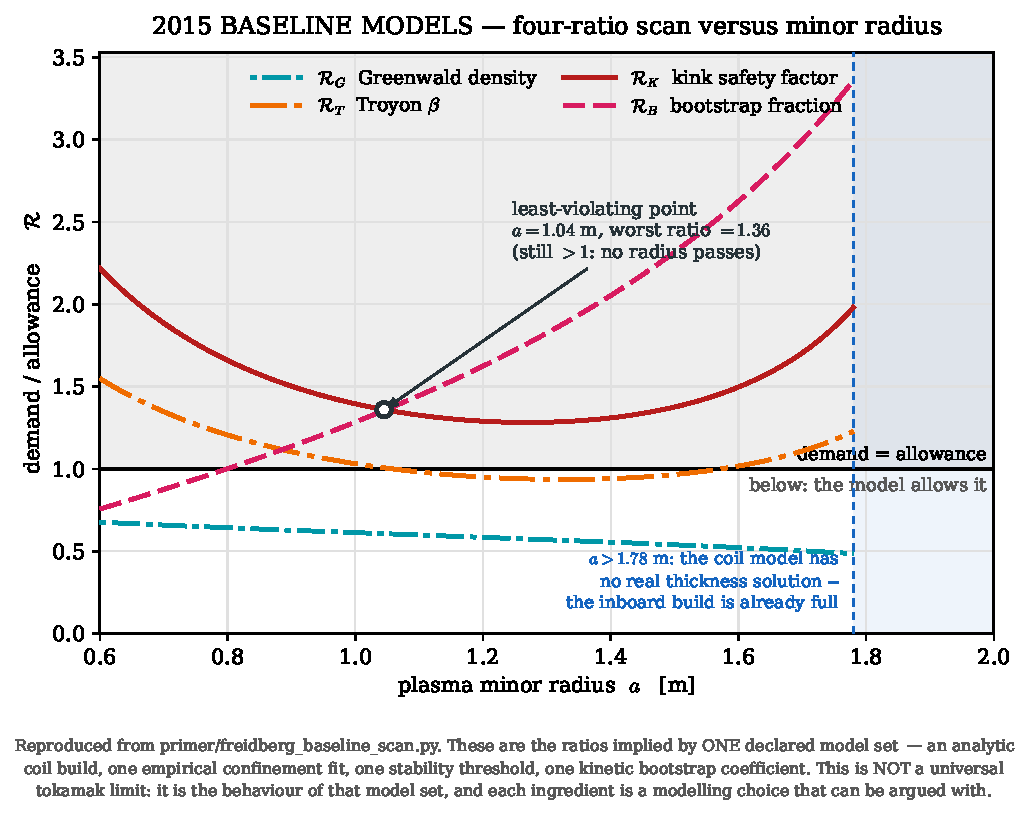
\includegraphics[width=1.0\textwidth]{figures/final/figS75_four_ratio_scan.pdf}
  \caption{Reset plot: reproducible four-ratio scan versus minor radius. \schematicnote}
  \label{fig:figS75_four_ratio_scan}
\end{figure}


% ============================= PAGE 76 ==============================
\newpage
\section*{76. The first conventional conclusion is conditional and specific}

We can now state precisely what has been demonstrated. Within the chosen mission,
wall-loading, blanket, TF-coil, confinement, lower-hybrid-current-drive,
standard-profile, and neoclassical-bootstrap models, changing conventional tokamak
size alone does not close both the kink and steady-state current requirements.

This is a strong result, but it is not a slogan about fusion. It does \emph{not} prove
that conventional tokamaks cannot operate, that advanced scenarios cannot improve
profiles, or that a modern magnet system cannot alter the trade. It identifies the
two demands that any proposed remedy must address: lower the confinement-driven total
current, and/or increase the allowed current and field-line-twist margin without
merely transferring the burden to beta, wall loading, or recirculating power.

The next section of the 2015 paper tests remedies in a disciplined order. First it
asks what improved confinement ($H>1$) buys and what beta margin it costs. Second it
raises the engineering field ceiling $B_{\max}$---the point at which a modern
HTS-enabled magnet discussion becomes relevant. Only after those conventional
trade-offs are visible will the thesis introduce alternative aspect-ratio geometry.

\designconsequence{The conventional baseline has now earned the question ``what
changes the current closure?'' High field and HTS enter next as a response to a
calculated failure, not as an unmotivated technology preference.}

% ============================= PAGE 77 ==============================
\newpage
\section*{77. Remedy one: what an $H$ factor does and does not mean}

The first remedy in the 2015 paper does not add a new piece of hardware. It asks
whether the plasma can lose energy more slowly than the reference H-mode regression
predicts. Write that possibility honestly as
\begin{equation}
 \tau_E=H\tau_{E,\rm ref},\qquad H>1.
 \label{eq:h-factor-definition}
\end{equation}
The symbol $H$ is a measured-performance multiplier relative to the particular
regression on page 58. It is not a new conservation law, a material property, or a
guarantee that a reactor can be run at the stated value.

There is nevertheless a physical picture behind trying it. Turbulent eddies carry
heat and particles down their gradients. Carefully shaped pressure and current
profiles can, in favorable regimes, change the magnetic shear and flow environment
felt by those eddies; an internal or edge transport barrier can then reduce the
effective outward transport. Maintaining such a state requires profile control and
must be demonstrated in the relevant operating regime. In an ignited plasma, alpha
heating also makes that control problem less independent than it is in an
externally heated experiment.

\imagebrief{Reset physics sketch: why an $H$ factor is not a knob on the machine}
{Draw a toroidal plasma cross-section only, with a broad radial temperature profile
on the left and a steeper, protected-gradient region on the right. Show small
outward turbulent heat arrows in the first case and shorter suppressed arrows in the
second. Label the second as a transport-barrier and profile-control empirical
performance change, not a new coil or reactor component. Do not add ST, HTS,
divertor, or a spherical plasma.}

\begin{figure}[htbp]\centering
  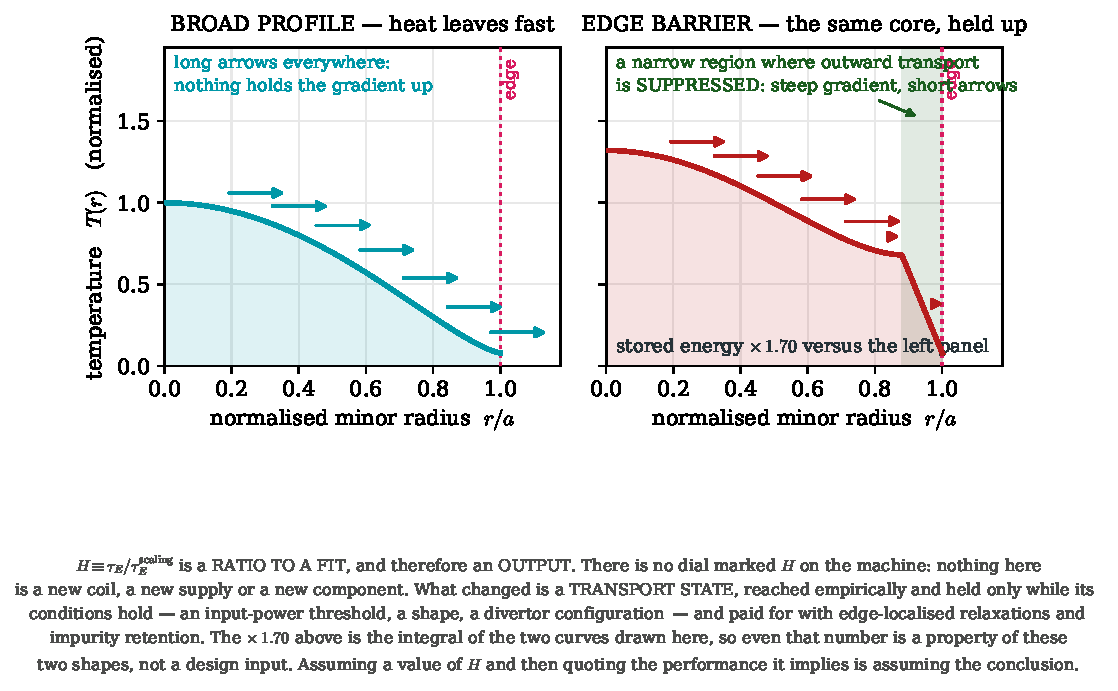
\includegraphics[width=1.0\textwidth]{figures/final/figS_h_factor.pdf}
  \caption{Reset physics sketch: why an $H$ factor is not a knob on the machine. \schematicnote}
  \label{fig:figS_h_factor}
\end{figure}


\model{Raising $H$ means assuming a better-than-reference confinement state and then
testing its consequences. It is a scenario assumption with experimental burden of
proof, not an available design margin.}
% ============================= PAGE 78 ==============================
\newpage
\section*{78. Better confinement lowers current---and moves every coupled test}

Equation~\eqref{eq:ireq-from-confinement} contains $H$ only in the denominator
inside a power $1/0.93$. Holding the other inputs of that equation fixed gives
\begin{equation}
 I_{\rm req}(H)=I_{\rm req}(1)\,H^{-1/0.93}.
 \label{eq:h-current-scaling}
\end{equation}
Thus a larger $H$ lowers the current that the empirical fit demands. Since
$q_*\propto1/I$ at fixed geometry,
\begin{equation}
 q_*(H)=q_*(1)\,H^{1/0.93}.
 \label{eq:h-q-scaling}
\end{equation}
This is the intended benefit: less current produces more field-line twist and hence
more margin in the adopted kink test.

But the same reduced current tightens two allowance ratios. The Greenwald allowance
is proportional to $I$, and the adopted Troyon pressure allowance is also
proportional to $I$. At fixed geometry and fusion pressure,
\begin{equation}
 \mathcal R_G(H)=\mathcal R_G(1)H^{1/0.93},\qquad
 \mathcal R_T(H)=\mathcal R_T(1)H^{1/0.93}.
 \label{eq:h-density-beta-scaling}
\end{equation}
In words: lowering current helps kink safety but makes a fixed density and pressure
look larger relative to current-based operating boundaries.

Bootstrap closure shifts in the helpful direction at fixed geometry. From
Eq.~\eqref{eq:freidberg-bootstrap-fraction}, $f_{\rm NC}\propto p/I^2$, while
$f_B=1-I_{\rm CD}/I$. Lower $I$ both raises the calculated bootstrap fraction and
reduces the required bootstrap share if the current-drive allowance is held fixed.
That is why increasing $H$ can remove the two original current-closure failures.
It cannot be called a solution until the density and beta checks are repeated.

\designconsequence{Improved confinement is not a free improvement. It trades a
current-and-kink problem for reduced current-based density and beta headroom. The
only fair test is a simultaneous recalculation.}

% ============================= PAGE 79 ==============================
\newpage
\section*{79. The $H$ scan: close bootstrap first, then inspect the remaining margins}

For each trial $H$, the 2015 procedure chooses the radius that closes the
steady-state current ledger:
\begin{equation}
 f_B\bigl(a,H\bigr)=f_{\rm NC}\bigl(a,H\bigr).
 \label{eq:h-bootstrap-match}
\end{equation}
This does not make the design acceptable; it simply removes one degree of freedom
before the other ratios are tested. The same transparent calculation file used for
the size scan now evaluates this condition, using the changed current in the
defining safety-factor relation rather than reusing a baseline $q_*$.

\begin{center}
\begin{tabular}{c c c c c c}
$H$ & $a$ (m) & $\mathcal R_G$ & $\mathcal R_T$ & $\mathcal R_K$
& $\mathcal R_B$\\
\hline
1.00 & 0.799 & 0.64 & 1.21 & 1.66 & 1.00\\
1.10 & 0.990 & 0.68 & 1.15 & 1.26 & 1.00\\
1.20 & 1.167 & 0.72 & 1.17 & 1.06 & 1.00\\
1.26 & 1.263 & 0.74 & 1.20 & 1.00 & 1.00\\
1.30 & 1.323 & 0.75 & 1.24 & 0.97 & 1.00\\
1.40 & 1.459 & 0.78 & 1.37 & 0.93 & 1.00
\end{tabular}
\end{center}

The table exhibits the trade directly. Near $H=1.26$, bootstrap and kink closure
are both obtained and the Greenwald ratio remains below one, but the Troyon ratio
is about $1.20$: the selected $2.8\%$ normalized-beta allowance is exceeded. Larger
$H$ only increases that beta demand in this family.

\auditnote{The paper reports the same qualitative conclusion and quotes a still
larger required normalized beta, $3.6\%$ rather than $2.8\%$, at its threshold
case. The printed analytic ledger reproduced here gives approximately $3.37\%$ on a
$10^{-3}\,\mathrm m$ radius grid. Both exceed $2.8\%$. We retain the discrepancy
rather than silently tune a coefficient to reproduce a prose number: the published
paper does not supply the full numerical implementation behind its figure.}

% ============================= PAGE 80 ==============================
\newpage
\section*{80. What the advanced-confinement remedy has established}

The $H$ exercise has sharpened the diagnosis. If an advanced transport state were
reliably available, it could lower the confinement-driven current enough to close
the baseline kink and bootstrap ledgers. In the declared conventional family, it
does so by asking the plasma to operate above the adopted normalized-beta allowance.
The missing quantity is not an unexplained new component; it is MHD pressure margin.

This is a useful result even if future experiments improve that margin. It tells us
exactly what must be supplied together: reproducible confinement enhancement,
profile control, and an MHD-stability basis for the higher normalized beta. Calling
only the first item the solution would conceal the coupled demand.

The next remedy changes a different primitive constraint: the maximum field that the
inboard TF system can bear. Higher field changes the required current, the current
drive efficiency, and the MHD ratios without assuming $H>1$. That is the logical
place to introduce high-temperature superconductors: first establish what a higher
$B_{\max}$ buys in this model, then ask whether an HTS magnet can provide it while
surviving its structural, thermal, and manufacturing constraints.

\designconsequence{The advanced-confinement route is a conditional plasma-physics
remedy, not a completed reactor design. The high-field route will be tested next as
a distinct engineering remedy, with its cost and stress penalties kept visible.}

% ============================= PAGE 81 ==============================
\newpage
\section*{81. Friedberg's second remedy: raise the field ceiling, not the confinement claim}

The preceding remedy changed the empirical confinement multiplier $H$. Friedberg's
second remedy holds $H=1$ and changes an engineering input instead: the maximum
magnetic field allowed at the inboard TF coil, $B_{\max}$. This is a clean
counterfactual. It asks what the already-derived conventional machine would demand if
its coil system could credibly tolerate a higher peak field.

At a fixed trial geometry, the immediate result is already known from
Eq.~\eqref{eq:b0radialbuild}, or from the source convention
Eq.~\eqref{eq:freidberg-b0-scan}:
\begin{equation}
 B_0=B_{\max}(1-\epsilon_B).
 \label{eq:high-field-b0}
\end{equation}
The central field consequently rises in direct proportion to the inboard field
ceiling if the fractional radial build is held fixed. The plasma pressure required by
the mission does not disappear. By the definition of beta,
\begin{equation}
 \beta=\frac{2\mu_0p}{B_0^2}.
 \label{eq:high-field-beta-definition}
\end{equation}
Thus at fixed pressure and geometry, doubling $B_0$ quarters $\beta$. This is the
first reason high field can relieve a pressure-stability problem: it increases the
magnetic pressure available to balance the same plasma pressure.

The reference compact expression for beta had $13\,\mathrm T$ absorbed into its
numerical coefficient. To vary $B_{\max}$ honestly, restore that dependence:
\begin{equation}
 \beta(\%)=
 \frac{1.31}{a^{1/2}(1-\epsilon_B)^2}
 \left(\frac{13\,\mathrm T}{B_{\max}}\right)^2.
 \label{eq:high-field-beta-scan}
\end{equation}
Equation~\eqref{eq:high-field-beta-scan} is not a new plasma law; it is
Eq.~\eqref{eq:high-field-beta-definition} after the 2015 power-and-size relations
have been substituted. Writing the factor explicitly prevents a common audit error:
one must not use a coefficient calibrated at $13\,\mathrm T$ unchanged in a
high-field scan.

\supportingquantity{raised field ceiling $B_{\max}$}{This is an engineering input,
not a new primary Friedberg parameter. It changes the primary central field $B_0$ and
the coil build $c$, then indirectly changes the current, stability, and
current-drive calculations.}

% ============================= PAGE 82 ==============================
\newpage
\section*{82. What field can help---and what it cannot help by itself}

First hold geometry fixed as a thought experiment. The selected confinement regression
gave the compact current requirement
\[
 I_{\rm req}\propto B_0^{-0.16}.
\]
The exponent is weak: a field increase alone reduces the regression's current demand,
but not dramatically. The more consequential changes occur after the current, safety
factor, current-drive, bootstrap, and radial-build relations are recalculated
together.

The safety-factor relation makes one helpful direction visible without any empirical
claim:
\begin{equation}
 q_*\propto\frac{a^2B_0}{R_0I}.
 \label{eq:high-field-q-direction}
\end{equation}
At unchanged geometry and current, a higher toroidal field increases field-line twist.
If the confinement relation also permits a lower current, the two effects both raise
$q_*$. Thus high field can address the same kink failure that improved confinement
addressed, but it does so through a different physical lever.

There is no free magnetic pressure. The field energy density and representative
mechanical stress scale are
\begin{equation}
 u_B=p_B=\frac{B_{\max}^2}{2\mu_0}.
 \label{eq:high-field-stress}
\end{equation}
This is the same result derived on page 47, now applied to the proposed remedy.
Higher field means larger Lorentz loads and, for a fixed allowable stress, more
structure. The source's analytic coil model calculates this response as a larger
$c$, rather than assuming that a better superconductor can make the support material
vanish.

\designconsequence{Raising $B_{\max}$ is physically promising because it lowers beta
and tends to raise $q_*$. It is physically expensive because the very field that
helps the plasma makes the coil's magnetic pressure grow as $B_{\max}^2$. The scan
must retain both statements.}

\imagebrief{Reset physics sketch: a stronger inboard field changes two ledgers}{Show
a conventional inboard midplane radial cut, not a new machine. Left branch:
$B_{\max}\uparrow\Rightarrow B_0\uparrow\Rightarrow\beta=2\mu_0p/B_0^2\downarrow$
and $q_*\propto B_0/I\uparrow$. Right branch:
$B_{\max}\uparrow\Rightarrow p_B=B_{\max}^2/(2\mu_0)\uparrow\Rightarrow$ greater
support demand and coil build $c$. Mark the right branch as a mechanical consequence,
not a drawback that superconductivity erases. No ST or divertor.}

\begin{center}\small\itshape
This brief asks for the two-sided field diagram that Figure~\ref{fig:figS_field_two_sided} already carries; its right branch is identical and its left differs only by two further nodes. Under the standing rule that redundancy is fixed rather than expanded, no second figure is drawn --- the extra nodes belong on that figure, and this brief should be retired.
\end{center}


% ============================= PAGE 83 ==============================
\newpage
\section*{83. Why field also changes the selected current-drive calculation}

The reference current ledger limits externally driven current because wave power is
limited. Its lower-hybrid model does not treat current-drive efficiency as a constant:
\begin{equation}
 \eta_{\rm CD}\simeq\frac{1.2}{n_\parallel^2},\qquad
 I_{\rm CD}=\frac{P_{\rm CD}\eta_{\rm CD}}{R_0\bar n}.
 \label{eq:high-field-current-drive}
\end{equation}
Here $n_\parallel\equiv ck_\parallel/\omega$ is the parallel refractive index of the
launched wave. In the selected outside-launch approximation it contains the ratio
\begin{equation}
 \frac{\omega_{pe}}{\Omega_e},\qquad
 \omega_{pe}^2=\frac{ne^2}{\epsilon_0m_e},\qquad
 \Omega_e=\frac{eB}{m_e}.
 \label{eq:high-field-frequency-ratio}
\end{equation}
The first expression measures the electron-plasma oscillation rate; the second is
the electron cyclotron rate. At fixed density, increasing local $B$ increases
$\Omega_e$ and decreases $\omega_{pe}/\Omega_e$. In this particular lower-hybrid
launch model, the resulting change in $n_\parallel$ improves the available
current-drive efficiency. That improvement reduces the bootstrap share required by
the ledger
\[
 f_B=1-\frac{I_{\rm CD}}{I}.
\]

This is a model-dependent bridge between magnet field and steady-state current. It
must not be generalized into the claim that every wave system becomes more efficient
at higher field. Launch geometry, accessibility, damping, parasitic absorption,
current profile, and the power plant's recirculating-power budget all require a
separate calculation.

\model{For Section 6.2 we keep Friedberg's $40\,\mathrm{MW}$ wave-power allocation,
its lower-hybrid accessibility model, its profiles, and $H=1$. We change only
$B_{\max}$ and then repeat the whole coupled calculation. This isolates what the
high-field proposal actually claims.}

% ============================= PAGE 84 ==============================
\newpage
\section*{84. The high-field scan: one closure condition, then four independent tests}

For every trial $B_{\max}$, retain the mission and wall-loading relations, compute
$R_0(a)$, $B_0(a,B_{\max})$, the analytic TF build $c$, pressure, density,
confinement-demanded current, lower-hybrid drive, and bootstrap fraction. As in the
$H$ scan, choose the remaining radius by the steady-state closure condition
\begin{equation}
 f_B(a,B_{\max})=f_{\rm NC}(a,B_{\max}).
 \label{eq:bmax-bootstrap-match}
\end{equation}
Only after that bookkeeping condition is met do we inspect the Greenwald, Troyon,
kink, and bootstrap ratios. The procedure is implemented directly in
\texttt{code/calculations/freidberg\_baseline\_scan.py}; its radius grid is
$0.001\,\mathrm m$, so the last displayed digit should not be read as a precision
claim.

\begin{center}
\begin{tabular}{c c c c c c c c}
$B_{\max}$ (T) & $a$ (m) & $B_0$ (T) & $c$ (m) & $\mathcal R_G$
& $\mathcal R_T$ & $\mathcal R_K$ & $\mathcal R_B$\\
\hline
13.0 & 0.799 & 10.10 & 1.02 & 0.64 & 1.21 & 1.66 & 1.00\\
15.0 & 0.875 & 11.20 & 1.27 & 0.65 & 1.00 & 1.30 & 1.00\\
17.0 & 0.944 & 12.19 & 1.55 & 0.65 & 0.85 & 1.06 & 1.00\\
17.6 & 0.964 & 12.47 & 1.64 & 0.65 & 0.82 & 1.00 & 1.00\\
18.0 & 0.976 & 12.66 & 1.70 & 0.65 & 0.80 & 0.97 & 1.00\\
20.0 & 1.036 & 13.53 & 2.05 & 0.65 & 0.70 & 0.83 & 1.00
\end{tabular}
\end{center}

The table has a simple reading. Greenwald changes little along this
bootstrap-matched family. Troyon becomes comfortable before the threshold. The kink
ratio is the last ratio to fall to one. On this transparent grid the first all-pass
point is $B_{\max}=17.65\,\mathrm T$; rounding to the precision of the underlying
model gives about $17.6\,\mathrm T$, the threshold reported in the 2015 paper.

\auditnote{This is a conditional result, not a prediction of a built reactor. It says
that the selected 2015 confinement regression, current-drive model, bootstrap model,
and four boundaries overlap when the inboard field ceiling is raised to roughly
$17.6\,\mathrm T$. Changing those models may move the number; it does not remove the
need to test their overlap.}

% ============================= PAGE 85 ==============================
\newpage
\section*{85. The price is measurable: more engineered volume and more exhaust burden}

The increasing $c$ column is already a direct mechanical cost of high field. The
source also records two simple engineering figures of merit. Its engineered-volume
proxy is
\begin{equation}
 \frac{V_I}{P_E}=\frac{V_B+V_{\rm TF}}{P_E},
 \label{eq:freidberg-cost-proxy}
\end{equation}
where $V_B$ is blanket-region volume and $V_{\rm TF}$ is TF-coil volume in its
specified geometry. It is not a literal construction-price quotation. It is a
transparent proxy for how much highly engineered blanket and magnet material must be
provided per electric megawatt.

The source's parallel-heat-flux proxy follows the alpha power along the field:
\begin{equation}
 Q_\parallel=\frac{P_\alpha B_0}{R_0}.
 \label{eq:freidberg-parallel-heat-proxy}
\end{equation}
Its units are $\mathrm{MW\,T\,m^{-1}}$. The relation is a scaling measure, not a
divertor-surface heat-flux calculation; a later chapter must introduce scrape-off
layer width, magnetic expansion, radiation, and material limits before asking what a
plate can survive.

For the source's compared cases, moving from its advanced-confinement case at
$13\,\mathrm T$ to the high-field all-constraint case near $17.6\,\mathrm T$
increases $V_I/P_E$ from $1.07$ to $1.87\,\mathrm{m^3\,MW^{-1}}$ (about a factor
$1.75$) and reports $Q_\parallel=657\,\mathrm{MW\,T\,m^{-1}}$, about $1.30$ times
its advanced-confinement comparison case. These are source-reported model outputs;
we do not reverse-engineer extra precision from a plotted calculation whose full
implementation was not published.

\designconsequence{The high-field branch closes the selected plasma ratios only by
moving difficulty into magnet structure, engineered volume, and exhaust. That is not
a refutation of high field. It is the reason magnet technology and heat exhaust must
be developed as part of the same reactor, not treated as a footnote to plasma
performance.}

% ============================= PAGE 86 ==============================
\newpage
\section*{86. HTS is earned here: an enabler with a mechanical bill}

A superconductor is useful because below its operating critical surface---set by
temperature, magnetic field, current density, field angle, strain, and material
state---it can carry a large current with negligible DC electrical resistance. The
important engineering quantity is therefore not the slogan zero resistance. It is a
measured, margin-bearing critical-current surface
\[
 I_c=I_c(B,T,\theta,\varepsilon,\hbox{conductor architecture}).
\]
The conductor must remain below that surface throughout normal operation and credible
transients, while its stabilizer, insulation, joints where present, cryogenic system,
and protection system handle disturbances.

The $13\,\mathrm T$ reference model was deliberately a conventional-magnet
assumption. The preceding scan has now made a more precise statement: \emph{within
this conventional $H=1$ route and these four declared plasma tests}, its
$B_{\max}=13\,\mathrm T$ ceiling is insufficient, whereas a ceiling near
$17.6\,\mathrm T$ makes the selected constraints overlap. A credible high-field
conductor is therefore necessary for this particular remedy. It is not a theorem that
HTS is necessary for every fusion strategy.

Rare-earth barium copper oxide (REBCO), commonly called an HTS conductor, is a serious
candidate because it can retain useful current capability in fields and temperatures
where a conventional low-temperature-superconductor design is much more constrained.
This is no longer purely aspirational: a representative-scale REBCO TF model coil
was built and tested to $20.1\,\mathrm T$ peak field on conductor at $20\,\mathrm K$.
\footnote{Z. S. Hartwig \emph{et al.}, The SPARC Toroidal Field Model Coil
Program, open preprint, 2023: \url{https://arxiv.org/abs/2308.12301}. The report
also records $40.5\,\mathrm{kA}$ terminal current, large Lorentz loading, and nearly
$1\,\mathrm{GPa}$ structural-case stress.}

That last fact is the corrective to magical thinking. HTS can open a higher
$B_{\max}$ window; it does not repeal Eq.~\eqref{eq:high-field-stress}. A fusion
magnet program must still close stress and strain, quench detection and energy
extraction, radiation tolerance, joint resistance where demountability is desired,
manufacturing yield, cryogenic power, inspection, and replacement. The next sections
remain in Friedberg's conventional design space; only after its closure problem is
fully mapped will the thesis ask whether a changed aspect ratio can solve a different
geometric problem.

\imagebrief{Cumulative high-field design state: the inboard TF system now has a
technology requirement}{Use cumulative state 13, preserving its conventional tokamak
geometry. In the inboard TF-coil bracket $c$, distinguish winding pack, structural
case, insulation/cooling, and the nuclear island $b$. Add a callout:
high-field branch requires a conductor technology whose operating critical-current
margin supports $B_{\max}\gtrsim17.6\,\mathrm T$. Put force arrows on the structural
case and state explicitly that HTS does not remove them. Do not introduce ST geometry
or a divertor.}

\begin{figure}[htbp]\centering
  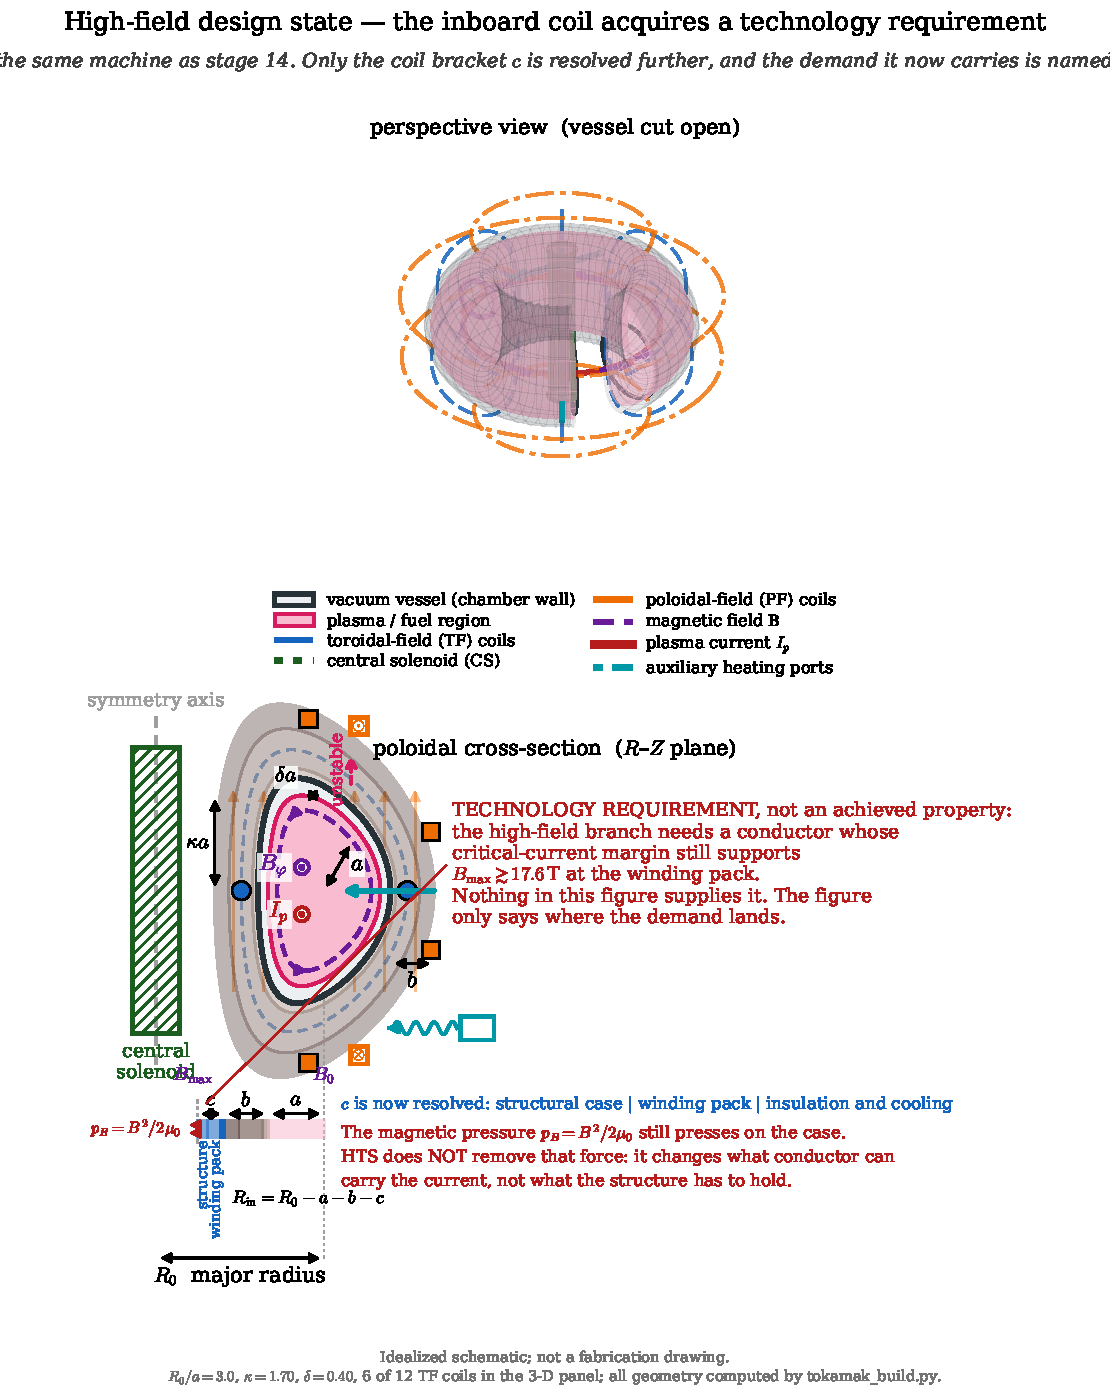
\includegraphics[width=1.0\textwidth]{figures/final/figM15_highfield_tall.pdf}
  \caption{The same machine as the previous state; only the coil bracket $c$ is resolved further, into structural case, winding pack and insulation/cooling. The field threshold is drawn as a REQUIREMENT on a conductor, not as a property the machine now has, and the force arrows stay: HTS changes what carries the current, not what the case must hold.}
  \label{fig:figM15_highfield_tall}
\end{figure}


% ============================= PAGE 87 ==============================
\newpage
\section*{87. Friedberg's third remedy: change the plant scale}

The high-field route changed a magnet limit. The next route changes a mission input:
the requested electric output $P_E$. The reference case chose
$P_E=1000\,\mathrm{MW_e}$. Raising that number may sound like making the problem
harder, because a larger plant must make more fusion power. At fixed allowed neutron
wall loading, however, it first forces a larger wall area:
\begin{equation}
 R_0a=
 7.16\left(\frac{P_E}{1000\,\mathrm{MW}}\right)\mathrm{m^2},
 \label{eq:power-scan-wall-product}
\end{equation}
where the coefficient retains the 2015 blanket, shape, wall-loading, and thermal
conversion assumptions.

The equation has an immediate geometrical meaning. For a chosen $a$, raising output
raises $R_0$ in proportion. The machine gains toroidal length and plasma volume
rather than being asked to generate arbitrarily more power per square metre of first
wall. This is the physical content behind the familiar phrase economy of scale. It
is not an accounting trick and it is not free: the absolute amount of plant,
inventory, construction, and grid-connected power also grows.

For this test Friedberg holds the original plasma and magnet assumptions:
\[
 H=1,\qquad B_{\max}=13\,\mathrm T,\qquad W_n=4\,\mathrm{MW\,m^{-2}},
\]
and again uses $f_B=f_{\rm NC}$ to select the compatible $a$ for each trial output.
The purpose is narrow: discover whether scale alone can make the four chosen
plasma-model constraints overlap without asserting better confinement or a
higher-field magnet.

% ============================= PAGE 88 ==============================
\newpage
\section*{88. More output at fixed wall loading means more volume, not higher pressure}

At the fixed temperature and profiles of the reference model, fusion power has the
form
\begin{equation}
 P_{\rm fus}\propto p^2V.
 \label{eq:power-scan-fusion-scaling}
\end{equation}
For a torus of fixed elongation, $V\propto R_0a^2$. Insert
Eq.~\eqref{eq:power-scan-wall-product}:
\[
 V\propto (R_0a)a\propto P_Ea.
\]
The thermal fusion power is proportional to $P_E$, so
\[
 P_E\propto p^2(P_Ea)
 \quad\Longrightarrow\quad
 p\propto a^{-1/2}.
 \label{eq:power-scan-pressure-cancellation}
\]
The factor $P_E$ cancels. At fixed $a$, the mission asks for a proportionally larger
volume at proportionally larger power, leaving the required average pressure
unchanged. With the fixed $T\simeq14\,\mathrm{keV}$ model and $p=2nT$, the same is
true of the average density:
\[
 n\propto a^{-1/2}.
\]

The confinement time makes the cancellation visible a second way. The stored thermal
energy scales as $W\sim pV\propto P_Ea^{1/2}$, while alpha heating scales as
$P_\alpha\propto P_E$. Thus
\begin{equation}
 \tau_{E,\rm req}=\frac{W}{P_\alpha}\propto a^{1/2},
 \label{eq:power-scan-taue-cancellation}
\end{equation}
again with no direct $P_E$ dependence at fixed $a$.

\designconsequence{Higher output at fixed wall loading does not buy lower pressure
by itself. It buys a larger volume in which to produce the larger total power. The
benefit, if any, must enter through the way that larger $R_0$ changes the
confinement-driven current and the current ledger.}

\imagebrief{Reset physics sketch: scale at fixed neutron wall loading}{Draw two
conventional torus silhouettes at the same labelled wall loading $W_n$. The right
machine has larger $R_0$, larger wall area, and proportionally larger $P_E$; keep the
plasma cross-section and pressure shading comparable. Beside it show the short chain
$P_E\uparrow\Rightarrow R_0a\uparrow\Rightarrow V\uparrow$ and
$P_E\propto p^2V\Rightarrow p$ unchanged at fixed $a$. This is a reset scaling sketch,
not a claim that large plants are automatically economical. No ST, HTS, or divertor.}

\begin{figure}[htbp]\centering
  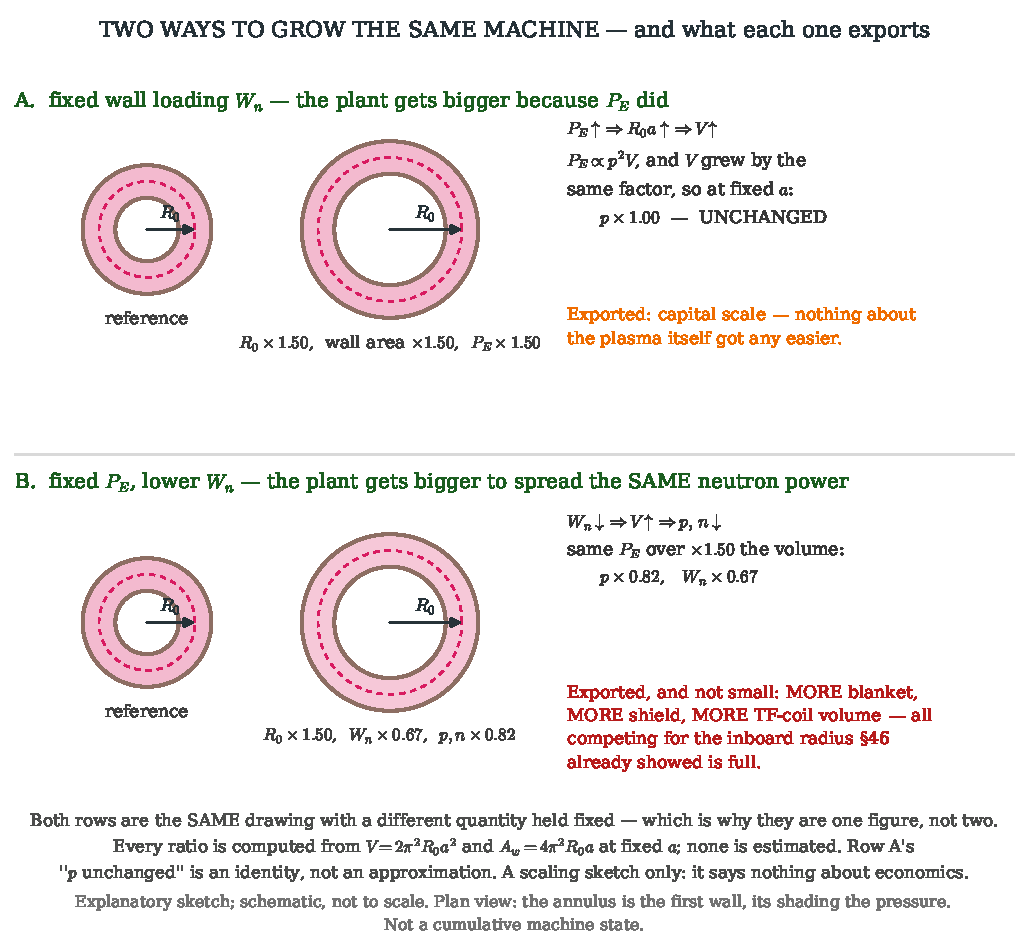
\includegraphics[width=1.0\textwidth]{figures/final/figS_scale_two_ways.pdf}
  \caption{Two ways to grow the same machine. Row A is this brief (fixed $W_n$); row B is the brief on lower wall loading. They are one figure because they are the same drawing with a different quantity held fixed --- and only side by side can the two chains be compared.}
  \label{fig:figS_scale_two_ways}
\end{figure}


% ============================= PAGE 89 ==============================
\newpage
\section*{89. The enlarged machine changes the current requirement}

The selected confinement relation, solved for current on page 59, has the dependence
\[
 I^{0.93}\propto
 \frac{\tau_{E,\rm req}P_\alpha^{0.69}}
 {R_0^{1.39}a^{0.58}n^{0.41}B_0^{0.15}}.
\]
At fixed $a$, the preceding page showed that $\tau_{E,\rm req}$ and $n$ do not carry
a direct power-output factor. In contrast,
\[
 P_\alpha^{0.69}\propto P_E^{0.69},
\qquad
 R_0^{1.39}\propto P_E^{1.39}.
\]
Ignoring for one line the smaller change in $B_0$ caused by the changed radial
geometry, their ratio is $P_E^{-0.70}$. Raising both sides to $1/0.93$ gives
\begin{equation}
 I_{\rm req}\propto P_E^{-0.70/0.93}
\simeq P_E^{-0.75}.
 \label{eq:power-scan-current-direction}
\end{equation}
This is the central mechanism of the power-output remedy. The larger major radius
helps the empirical confinement scaling more strongly than the increased alpha power
hurts it, so the regression asks for less current at a fixed cross-section.

The current-drive budget must be updated at the same time. If the selected
recirculating-power fraction remains fixed, $P_{\rm CD}\propto P_E$. But
\[
 I_{\rm CD}=\frac{P_{\rm CD}\eta_{\rm CD}}{R_0n}
\]
contains the same factor $R_0\propto P_E$ in its denominator. At fixed $a$ its direct
power dependence approximately cancels, leaving field and wave-accessibility changes
to determine the remainder. The required total current, however, falls according to
Eq.~\eqref{eq:power-scan-current-direction}. Therefore the bootstrap fraction
required by the ledger falls:
\[
 f_B=1-\frac{I_{\rm CD}}{I}.
\]
This is why a larger plant can ease both the kink test and steady-state closure in
the stated model. It is not because a large reactor creates bootstrap current from
nothing.

\model{The exponent $-0.75$ is a consequence of the selected empirical confinement
fit, fixed wall loading, fixed temperature/profiles, and a fixed recirculating-power
fraction. It is a transparent model implication, not a size-scaling theorem for all
tokamaks.}

% ============================= PAGE 90 ==============================
\newpage
\section*{90. The power-output scan: the model closes near $1.55\,\mathrm{GW_e}$}

For each $P_E$, the calculation holds $H=1$ and $B_{\max}=13\,\mathrm T$, imposes
$f_B=f_{\rm NC}$, and then tests all four ratios. The output and radius grids are
$1\,\mathrm{MW}$ and $0.001\,\mathrm m$ respectively.

\begin{center}
\begin{tabular}{c c c c c c c c}
$P_E$ (MW) & $a$ (m) & $R_0$ (m) & $B_0$ (T) & $\mathcal R_G$
& $\mathcal R_T$ & $\mathcal R_K$ & $\mathcal R_B$\\
\hline
1000 & 0.799 & 8.96 & 10.10 & 0.64 & 1.21 & 1.66 & 1.00\\
1200 & 1.030 & 8.34 & 9.52 & 0.71 & 1.09 & 1.31 & 1.00\\
1400 & 1.263 & 7.94 & 8.97 & 0.77 & 1.02 & 1.10 & 1.00\\
1550 & 1.436 & 7.73 & 8.57 & 0.81 & 0.99 & 1.00 & 1.00\\
1600 & 1.493 & 7.67 & 8.44 & 0.82 & 0.99 & 0.97 & 1.00\\
1800 & 1.717 & 7.51 & 7.95 & 0.87 & 0.97 & 0.89 & 1.00
\end{tabular}
\end{center}

The kink and Troyon ratios are the last two to close. The script's first all-pass
point is $P_E=1556\,\mathrm{MW}$ on its displayed grids; Friedberg reports
$1550\,\mathrm{MW}$, an agreement appropriate to a simplified model and discrete
scan. Greenwald remains below one with appreciable margin.

\auditnote{This result does not say that a $1.55\,\mathrm{GW_e}$ reactor is preferred,
financeable, grid-compatible, licensable, or buildable. It says only that raising
the output is a third way to make the stated four plasma-model inequalities overlap
while retaining $H=1$ and the paper's $13\,\mathrm T$ magnet assumption.}

% ============================= PAGE 91 ==============================
\newpage
\section*{91. A larger plant trades plasma closure for absolute scale and heat exhaust}

The source's engineered-volume proxy at the $1550\,\mathrm{MW_e}$ case is
\[
 \frac{V_I}{P_E}=1.17\,\mathrm{m^3\,MW^{-1}},
\]
close to its $1.07\,\mathrm{m^3\,MW^{-1}}$ advanced-confinement comparison. That is
the limited sense in which the source identifies an economy of scale: the engineered
volume \emph{per megawatt} need not rise sharply. It does not mean the total
engineering volume or capital required for a $1550\,\mathrm{MW_e}$ plant is small;
both are necessarily larger in absolute terms.

The same source reports its parallel-heat-flux proxy rising to
\[
 Q_\parallel=673\,\mathrm{MW\,T\,m^{-1}}
\]
at the high-output point, compared with $507\,\mathrm{MW\,T\,m^{-1}}$ in its
advanced-confinement comparison case. The proxy is a warning that core
plasma-constraint closure does not settle power exhaust. It is not a divertor design
calculation, and it must not be translated directly into a material surface limit.

\designconsequence{The third remedy establishes a genuine alternative within the
2015 model: conventional field and ordinary confinement can meet the four selected
plasma tests at a sufficiently large output. It also leaves us with a larger,
more-concentrated generating station and a more demanding exhaust proxy. A reactor
is not complete merely because one family of plasma ratios reaches one.}

% ============================= PAGE 92 ==============================
\newpage
\section*{92. Friedberg's fourth remedy: lower the permitted wall loading}

The last single-knob remedy changes the allowed average neutron wall loading $W_n$.
The reference value was $4\,\mathrm{MW\,m^{-2}}$. Lowering it means demanding a
larger first-wall area for the same neutron power:
\begin{equation}
 R_0a=
 7.16\left(\frac{4\,\mathrm{MW\,m^{-2}}}{W_n}\right)\mathrm{m^2}
 \qquad(P_E=1000\,\mathrm{MW_e}).
 \label{eq:wall-scan-wall-product}
\end{equation}
This is not an arbitrary way to make the plasma easier. It represents a conservative
nuclear-material and first-wall design choice: less neutron power is assigned to each
square metre, so more square metres must be built.

The immediate trade is visible before any plasma fit is used. At fixed $a$,
$R_0\propto W_n^{-1}$ and $V\propto R_0a^2\propto W_n^{-1}$. The same fusion output
is produced in a larger volume. That lowers the required power density, pressure, and
density, but it makes the reactor physically larger. Friedberg holds
\[
 P_E=1000\,\mathrm{MW_e},\qquad H=1,\qquad B_{\max}=13\,\mathrm T,
\]
and again imposes bootstrap closure to select $a(W_n)$ before testing the four
ratios.

\designconsequence{A lower wall-loading limit is not a plasma improvement supplied
for free. It is a decision to purchase lower power density with more wall, blanket,
shielding, magnets, and building-scale volume. The next pages quantify how that
engineering choice reaches the current problem.}

% ============================= PAGE 93 ==============================
\newpage
\section*{93. Lower wall loading reduces the required pressure}

At fixed output and temperature, use again
\[
 P_{\rm fus}\propto p^2V.
\]
From Eq.~\eqref{eq:wall-scan-wall-product}, $V\propto W_n^{-1}a$ at fixed
elongation. Holding total fusion power fixed therefore gives
\begin{equation}
 p\propto\left(\frac{W_n}{a}\right)^{1/2},\qquad
 n\propto\left(\frac{W_n}{a}\right)^{1/2}.
 \label{eq:wall-scan-pressure-density}
\end{equation}
Unlike the higher-output case, there is no cancellation: reducing $W_n$ genuinely
reduces the average pressure and density required to make the same total power.

The stored energy scales as
\[
 W\sim pV\propto
\left(\frac{W_n}{a}\right)^{1/2}\left(\frac a{W_n}\right)
=\left(\frac a{W_n}\right)^{1/2}.
\]
The alpha power is unchanged because the total fusion output is unchanged. Hence
\begin{equation}
 \tau_{E,\rm req}\propto\left(\frac a{W_n}\right)^{1/2}.
 \label{eq:wall-scan-taue}
\end{equation}
This longer required confinement time may look like a penalty, but it must be placed
beside the larger $R_0$, lower density, and changed field geometry in the empirical
confinement law before judging the net current demand.

\imagebrief{Reset physics sketch: lower wall loading trades density for machine
scale}{Draw two conventional torus silhouettes at the same $P_E$ and temperature.
The right machine has a larger $R_0$, more first-wall area, lower labelled $W_n$,
and lighter pressure/density shading. Show
$W_n\downarrow\Rightarrow V\uparrow\Rightarrow p,n\downarrow$, then the explicit
warning: more blanket, shield, and TF-coil volume. This is a reset scaling sketch,
not a cumulative machine state. No ST, HTS, or divertor.}

\begin{center}\small\itshape
This brief and the previous one ask for the same drawing with a different quantity held fixed, so they share one figure: see row~B of Figure~\ref{fig:figS_scale_two_ways}.
\end{center}


% ============================= PAGE 94 ==============================
\newpage
\section*{94. The net current direction follows from all terms together}

Use the same selected confinement dependence:
\[
 I^{0.93}\propto
\frac{\tau_{E,\rm req}P_\alpha^{0.69}}
{R_0^{1.39}a^{0.58}n^{0.41}B_0^{0.15}}.
\]
At fixed $a$, Eqs.~\eqref{eq:wall-scan-pressure-density} and
\eqref{eq:wall-scan-taue} give
\[
 \tau_{E,\rm req}\propto W_n^{-1/2},\qquad
 R_0^{-1.39}\propto W_n^{1.39},\qquad
 n^{-0.41}\propto W_n^{-0.205}.
\]
Multiplying the three explicit wall-loading powers gives
\[
 W_n^{-0.500+1.390-0.205}=W_n^{0.685}.
\]
Consequently,
\begin{equation}
 I_{\rm req}\propto W_n^{0.685/0.93}
\simeq W_n^{0.74},
 \label{eq:wall-scan-current-direction}
\end{equation}
apart from the smaller self-consistent change in $B_0$. Lowering wall loading lowers
the current demanded by the selected regression. It also lowers beta directly through
Eq.~\eqref{eq:wall-scan-pressure-density}, while the larger $R_0$ and lower current
improve the kink ratio in the full calculation.

External current drive deserves the same caution as before. With fixed output,
$P_{\rm CD}$ is fixed. As $W_n$ falls, $R_0n\propto W_n^{-1/2}$ grows, which tends to
reduce the externally driven current in the selected efficiency model. Yet
$I_{\rm req}$ falls more rapidly in this family; the required bootstrap share still
decreases after all quantities are recalculated. The conclusion is a coupled result,
not a consequence of holding $I_{\rm CD}$ fixed by hand.

% ============================= PAGE 95 ==============================
\newpage
\section*{95. The wall-loading scan closes near $2.1\,\mathrm{MW\,m^{-2}}$}

The calculation now scans $W_n$ while retaining $P_E=1000\,\mathrm{MW_e}$,
$H=1$, and $B_{\max}=13\,\mathrm T$. At each value it first sets
$f_B=f_{\rm NC}$ and then tests the same four ratios.

\begin{center}
\begin{tabular}{c c c c c c c c}
$W_n$ ($\mathrm{MW\,m^{-2}}$) & $a$ (m) & $R_0$ (m) & $B_0$ (T)
& $\mathcal R_G$ & $\mathcal R_T$ & $\mathcal R_K$ & $\mathcal R_B$\\
\hline
4.00 & 0.799 & 8.96 & 10.10 & 0.64 & 1.21 & 1.66 & 1.00\\
3.50 & 0.890 & 9.19 & 10.04 & 0.65 & 1.11 & 1.49 & 1.00\\
3.00 & 1.009 & 9.46 & 9.96 & 0.67 & 1.00 & 1.32 & 1.00\\
2.50 & 1.171 & 9.78 & 9.85 & 0.68 & 0.89 & 1.14 & 1.00\\
2.10 & 1.349 & 10.11 & 9.72 & 0.69 & 0.80 & 1.00 & 1.00\\
2.00 & 1.403 & 10.21 & 9.68 & 0.70 & 0.78 & 0.97 & 1.00
\end{tabular}
\end{center}

The kink criterion is again the final one to close. The transparent script finds the
largest all-pass wall loading as $2.09\,\mathrm{MW\,m^{-2}}$ on its displayed grids;
the source reports $W_n\lesssim2.1\,\mathrm{MW\,m^{-2}}$. This agreement is a
useful check on the algebra, not validation of every physical assumption beneath the
2015 model.

\auditnote{Lower wall loading can close the selected plasma constraints without
advanced confinement or a higher-field magnet. It does so by selecting a larger,
lower-power-density machine. Any claim that this is the best reactor strategy must
also compare its blanket, shield, coil, construction, maintenance, and financing
burden.}

% ============================= PAGE 96 ==============================
\newpage
\section*{96. The reward is lower exhaust proxy; the price is a much larger plant}

The source reports the low-wall-loading case's engineered-volume proxy as
\[
 \frac{V_I}{P_E}=2.59\,\mathrm{m^3\,MW^{-1}}
\]
near $W_n=2.1\,\mathrm{MW\,m^{-2}}$, compared with
$1.07\,\mathrm{m^3\,MW^{-1}}$ in its advanced-confinement comparison: about a
factor $2.42$ increase. This is qualitatively expected from the enlarged radial and
toroidal dimensions, though the exact number belongs to its specified blanket and
TF-coil geometry.

The reported parallel-heat-flux proxy moves in the favorable direction,
from $507$ to $374\,\mathrm{MW\,T\,m^{-1}}$ in those compared cases. Lower average
power density makes an exhaust problem less severe, but it does not solve it.
Divertor and first-wall design still require a separate calculation of power sharing,
scrape-off-layer transport, radiation, magnetic expansion, detachment, and material
response.

\designconsequence{The four single-variable remedies have now revealed four distinct
currencies: empirical confinement margin, magnet field and structure, plant output,
and neutron-wall area. Each can close the selected plasma ledger under stated
assumptions; each exports difficulty into another part of the reactor. The next task
is to compare the remedies on one honest ledger before moving beyond Friedberg's
conventional baseline.}

% ============================= PAGE 97 ==============================
\newpage
\section*{97. One comparison ledger: which changes actually close the four tests?}

The four options are not four versions of the same physical claim. Each changes one
declared input while retaining the others as closely as the coupled calculation
permits:

\begin{center}
\begin{tabular}{p{0.23\textwidth}p{0.29\textwidth}p{0.33\textwidth}}
\textbf{Option} & \textbf{Changed demand} & \textbf{Result in the stated model}\\
\hline
Improved confinement & $H:1\rightarrow1.26$ & Kink and bootstrap close, but the
Troyon ratio is about $1.20>1$; not a full closure.\\[3pt]
High field & $B_{\max}:13\rightarrow17.6\,\mathrm T$ & All four ratios close;
magnet stress, coil build, and engineered-volume proxy rise.\\[3pt]
Higher output & $P_E:1000\rightarrow1550\,\mathrm{MW_e}$ & All four ratios close;
absolute plant size and heat-exhaust proxy rise.\\[3pt]
Lower wall loading & $W_n:4\rightarrow2.1\,\mathrm{MW\,m^{-2}}$ & All four ratios
close; engineered volume per megawatt rises strongly.
\end{tabular}
\end{center}

The first row is deliberately retained. It teaches the method: finding one
simultaneous equality, such as $f_B=f_{\rm NC}$, is not enough. Every inequality must
be retested at the same state. The remaining three routes pass this particular
four-ratio screen only because the changed input alters the confinement-driven current,
the current ledger, and the pressure/stability ledger together.

\imagebrief{Reset comparison sketch: four ways to move the same current closure}{Draw
one compact causal map with a central block labelled required plasma current from the
empirical confinement fit. Four incoming branches: $H\uparrow$ (empirical transport
assumption); $B_{\max}\uparrow$ (field and structural demand); $P_E\uparrow$ at fixed
$W_n$ (larger plant); and $W_n\downarrow$ at fixed $P_E$ (larger lower-power-density
plant). Each branch must show a distinct exported burden. Mark $H=1.26$ as beta
failure, and the other three as four-ratio closure only within the stated 2015
models. This is a reset causal graphic, not a new machine drawing.}

\begin{figure}[htbp]\centering
  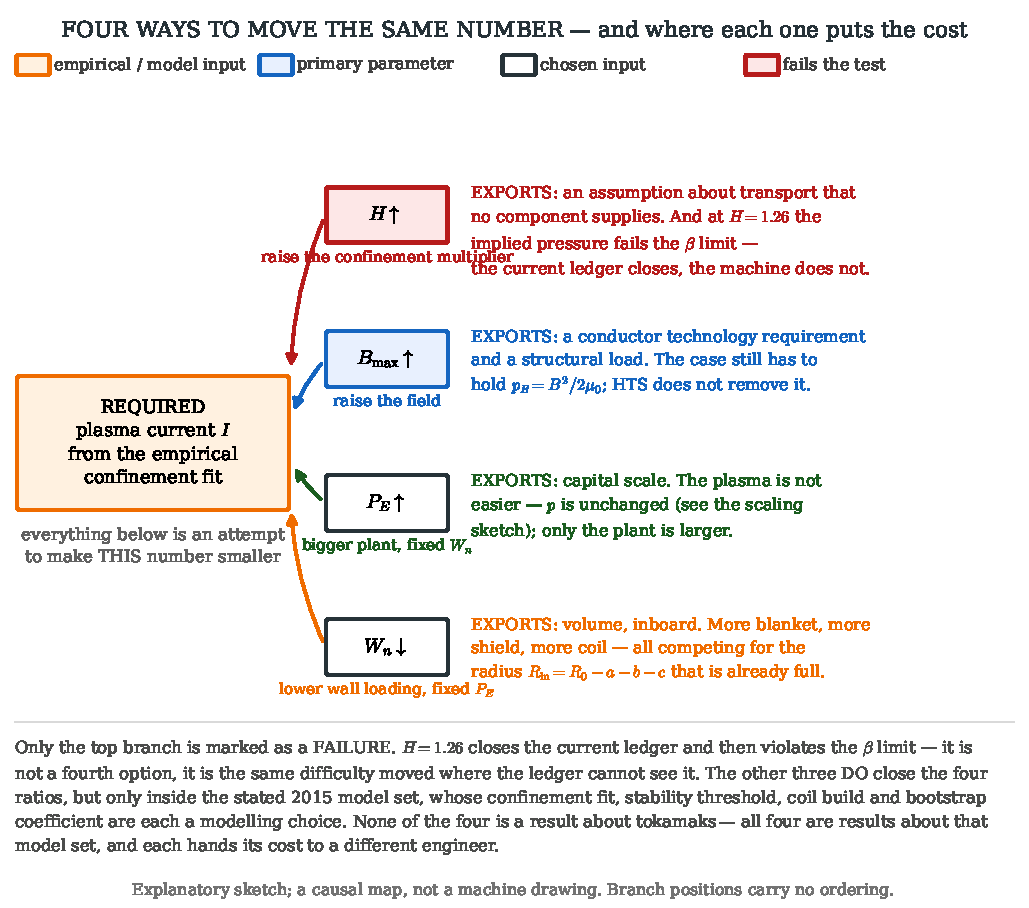
\includegraphics[width=1.0\textwidth]{figures/final/figS_four_ways_to_close.pdf}
  \caption{Reset comparison sketch: four ways to move the same current closure. \schematicnote}
  \label{fig:figS_four_ways_to_close}
\end{figure}


% ============================= PAGE 98 ==============================
\newpage
\section*{98. The source's final cases, stated without pretending to measure reality}

For orientation, the 2015 paper reports the following rounded states. The values are
not independent targets; they are outputs of its coupled equations after the listed
input change. The reference row is shown because it makes the original mismatch
visible.

\begin{center}
\begin{tabular}{c c c c c c}
 & reference & $H=1.26$ & high field & high output & low wall load\\
\hline
$B_{\max}$ (T) & 13 & 13 & 17.6 & 13 & 13\\
$P_E$ (MW) & 1000 & 1000 & 1000 & 1554 & 1000\\
$W_n$ ($\mathrm{MW\,m^{-2}}$) & 4.0 & 4.0 & 4.0 & 4.0 & 2.1\\
$a$ (m) & 1.34 & 1.26 & 0.97 & 1.44 & 1.35\\
$R_0$ (m) & 5.34 & 5.57 & 7.39 & 7.70 & 10.2\\
$I$ (MA) & 14.3 & 10.0 & 7.64 & 11.2 & 8.52\\
$q_K/q_*$ & 1.28 & 1.00 & 1.00 & 1.00 & 1.00\\
$f_B/f_{\rm NC}$ & 1.90 & 1.00 & 1.00 & 1.00 & 1.00\\
$\beta/\beta_T$ & 0.94 & 1.21 & 0.82 & 1.00 & 0.80
\end{tabular}
\end{center}

The table confirms three conceptual lessons. First, the reference failure is
current-centered: its $q_K/q_*$ and bootstrap ratio exceed one. Second, reducing
current is not sufficient if the way it is reduced also tightens the beta allowance,
as the $H=1.26$ row shows. Third, high field, plant scale, and low wall loading are
not interchangeable technologies; they reach current closure through different
geometric and engineering commitments.

\model{This table reproduces rounded values reported in the freely available 2015
source. Our companion script independently reproduces the three closure thresholds
to the resolution stated in the relevant scans. Neither result turns the source's
profile choices, empirical boundaries, or coil model into universally valid reactor
predictions.}

% ============================= PAGE 99 ==============================
\newpage
\section*{99. What Friedberg's calculation has rigorously established}

The word rigorously must be used carefully. The following implication has been
established by transparent substitution and numerical quadrature:
\[
\begin{array}{c}
\text{2015 mission, geometry, coil, profile, confinement, current-drive,}\\
\text{bootstrap, and four-limit assumptions}
\end{array}
\quad\Longrightarrow\quad
\begin{array}{c}
\text{the reference conventional state fails kink and}\\
\text{steady-state bootstrap closure simultaneously.}
\end{array}
\]
The size scan shows that merely choosing another minor radius within that baseline
does not make all four tests pass. The remedy scans then identify which changed
assumptions can restore overlap, and what new burden each imports.

What has \emph{not} been established is equally important. The calculation is not a
proof that every conventional tokamak fails, that any one high-field plant can be
built, or that a ratio below one makes a reactor safe. The Greenwald relation and
the chosen normalized-beta allowance are operational boundaries, not theorems. The
confinement and current-drive laws are empirical/model closures. The bootstrap result
depends on the chosen equilibrium and profiles. The analytic coil model is not a
detailed magnet design.

\designconsequence{The real achievement of the reconstruction is not a slogan about
tokamaks. It is a map of conditional causal failures: which physics assumption or
engineering choice causes each failure, what intervention can remove it in the model,
and what new design obligation is thereby created.}

% ============================= PAGE 100 ==============================
\newpage
\section*{100. Four ratios are not a complete reactor acceptance test}

The 2015 paper intentionally keeps several major reactor questions outside its
four-ratio screen. The most immediate is power exhaust. $Q_\parallel$ is only a
parallel-transport proxy; no scrape-off-layer width, divertor geometry, impurity
radiation, detachment window, transient load, or material lifetime has yet been
calculated. A passing value of $q_K/q_*$ is likewise not a complete disruption-risk
assessment. Vertical stability, control authority, error fields, energetic particles,
resistive walls, and nonlinear evolution are not exhausted by one edge safety factor.

On the engineering side, the radial-build calculation has identified why blanket,
shield, winding pack, and structure consume space, but it has not produced a
maintainable nuclear island. Neutron damage, tritium inventory, remote handling,
cryoplant electricity, joint reliability where relevant, fatigue, and component
replacement remain design problems. On the plant side, net electric output and
recirculating power must eventually be joined to availability, construction schedule,
licensing, fuel cycle, and grid integration.

None of these omissions invalidates the four-ratio argument. They prevent us from
misrepresenting it as a completed reactor design. The correct next move is to retain
the conventional baseline as a reference and ask whether a different aspect-ratio
geometry can improve the current-and-field trade \emph{without} hiding the radial
build and central-stack obligations it creates.

% ============================= PAGE 101 ==============================
\newpage
\section*{101. The conventional baseline is now complete enough to earn the next question}

We began without a tokamak and let the conventional machine reveal itself: a hot
charged fusion plasma required magnetic confinement; the escape direction required a
torus and TF coils; toroidal drifts required current, poloidal field, and shaping;
steady state required a current ledger; fusion neutrons required the nuclear island;
and the field required a finite inboard magnet build. The primary parameter set
\[
 a,\ R_0,\ \kappa,\ b,\ c,\ T,\ n,\ p,\ \tau_E,\ B_0,\ \beta,\ I,\ q_*,\ f_B
\]
has acquired physical meaning before it was used as engineering input.

Friedberg's reference calculation then exposed the conventional current closure:
under its declared assumptions, an ordinary reference machine needs too much current
for both its adopted kink margin and its available steady-state bootstrap share. The
high-field result gives HTS its correct causal position: it is a technology that can
open a needed field window in one closure route, while intensifying structural and
protection demands.

Only now is it legitimate to consider low-aspect-ratio, spherical-tokamak geometry.
It will not be introduced as a compact machine-shaped answer. It must first be asked
what aspect ratio changes in the same equations, which conventional failures it can
relieve, and why its reduced central space creates the central-stack problem. The
next chapter begins that comparison from the already-earned radial-build ledger.

% ============================= PAGE 102 ==============================
\newpage
\section*{102. A spherical tokamak changes one geometric ratio, not the laws of plasma}

Define the plasma aspect ratio by
\begin{equation}
 A\equiv\frac{R_0}{a}.
 \label{eq:aspect-ratio-definition}
\end{equation}
A conventional tokamak has $A$ of order $3$--$4$ or larger. A low-aspect-ratio
tokamak, commonly called a spherical tokamak (ST), has $A$ of order $1$--$2$.
The word spherical describes the compact toroidal shape; the plasma remains a torus,
not a filled sphere. It still needs TF field, poloidal field, equilibrium control,
heating, exhaust, a vacuum boundary, and a nuclear island.

At a fixed fusion mission and wall-loading product $R_0a=C_{\rm wall}$, the two
geometric variables can instead be written in terms of $A$:
\begin{equation}
 R_0=(AC_{\rm wall})^{1/2},\qquad
 a=\left(\frac{C_{\rm wall}}A\right)^{1/2}.
 \label{eq:aspect-ratio-wall-geometry}
\end{equation}
Thus lowering $A$ makes the cross-section larger while bringing the plasma centre
closer to the symmetry axis. It is not simply a uniformly shrunken conventional
machine.

\designconsequence{Aspect ratio is a causal geometric variable. Lowering it can alter
field-line twist, trapped-particle physics, volume, and radial space at once. We must
derive each direction separately before calling low aspect ratio an advantage.}

\imagebrief{Reset geometry sketch: aspect ratio changes the torus, not the physics
inventory}{Show two midplane cuts with the same labelled $R_0a=C_{\rm wall}$:
a conventional $A\simeq4$ plasma and a low-$A\simeq1.5$ plasma. Mark $R_0$, $a$,
and the symmetry axis. Retain only the already-earned plasma, nuclear-island bracket,
and TF-system location as simplified outlines. Make the low-A inboard gap visibly
smaller. Do not label either design as automatically superior and do not yet add an
HTS brand or an ST-specific divertor.}

\begin{figure}[htbp]\centering
  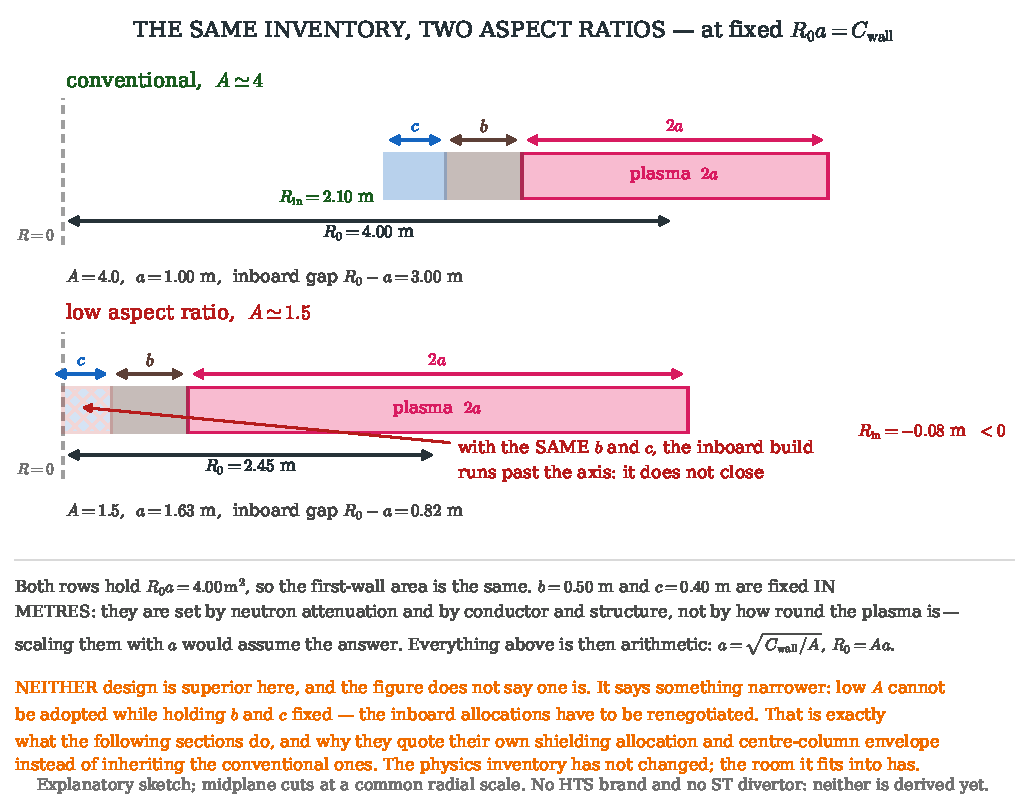
\includegraphics[width=1.0\textwidth]{figures/final/figS_aspect_ratio_geometry.pdf}
  \caption{Reset geometry sketch: aspect ratio changes the torus, not the physics inventory. \schematicnote}
  \label{fig:figS_aspect_ratio_geometry}
\end{figure}


% ============================= PAGE 103 ==============================
\newpage
\section*{103. Low aspect ratio strengthens toroidal field variation and trapping}

The toroidal-field relation remains
\[
 B_\varphi(R)R=B_0R_0.
\]
At the inboard and outboard plasma edges, $R=R_0-a$ and $R=R_0+a$. Hence
\begin{equation}
 \frac{B_{\rm out}}{B_{\rm in}}
 =\frac{R_0-a}{R_0+a}
 =\frac{A-1}{A+1}.
 \label{eq:aspect-ratio-field-variation}
\end{equation}
When $A$ falls, this ratio falls: the inboard field becomes much stronger than the
outboard field. The mirror argument from page 36 then says that a larger fraction of
particles can be trapped. In the simple low-collisionality estimate used earlier,
\begin{equation}
 f_t\simeq
 \left(1-\frac{B_{\min}}{B_{\max}}\right)^{1/2}
 \simeq\left(\frac{2}{A+1}\right)^{1/2}.
 \label{eq:aspect-ratio-trapped-fraction}
\end{equation}
For orientation, this expression gives $f_t\simeq0.63$ at $A=4$ and
$f_t\simeq0.89$ at $A=1.5$.

More trapped particles make a larger bootstrap response physically plausible because
bootstrap current begins with trapped-particle/passing-particle collisional
asymmetry. But Eq.~\eqref{eq:aspect-ratio-trapped-fraction} is not a bootstrap
fraction. The large-aspect-ratio local closure used on pages 67--70 is no longer
controlled at $A\sim1$--$2$. A finite-aspect-ratio kinetic calculation must replace
it before claiming a numerical $f_{\rm NC}$ for an ST.

\model{The direction of the trapping effect follows from the toroidal-field geometry
and magnetic-moment argument. The resulting bootstrap fraction, profile, and
collisionality dependence are finite-aspect-ratio neoclassical physics, not a number
that can be extrapolated from Freidberg's large-aspect-ratio coefficient.}

% ============================= PAGE 104 ==============================
\newpage
\section*{104. Aspect ratio also changes the kink--beta coupling}

The shaped edge safety-factor estimate was
\begin{equation}
 q_*=
\frac{2\pi a^2B_0}{\mu_0R_0I}
\left(\frac{1+\kappa^2}{2}\right)
=\frac{2\pi}{\mu_0}
\left(\frac{1+\kappa^2}{2}\right)
\frac{aB_0}{AI}.
 \label{eq:aspect-ratio-q}
\end{equation}
Normalized beta contains the same dimensional group $aB_0/I$:
\begin{equation}
 \beta_N\equiv
\beta(\%)\frac{aB_0}{I_{\rm MA}}.
 \label{eq:aspect-ratio-beta-n}
\end{equation}
Here $I_{\rm MA}=I/(10^6\,\mathrm A)$ and $\beta(\%)=100\beta$. Substitute
\[
 \frac{aB_0}{I}
=\frac{\beta_N}{10^8\beta}
\]
into Eq.~\eqref{eq:aspect-ratio-q} to obtain
\begin{equation}
 q_*=
\frac{0.05}{A}
\left(\frac{1+\kappa^2}{2}\right)
\frac{\beta_N}{\beta}.
 \label{eq:aspect-ratio-q-beta}
\end{equation}
The numerical $0.05$ comes only from $\mu_0=4\pi\times10^{-7}$ and the conventional
percent--MA units in $\beta_N$.

Equation~\eqref{eq:aspect-ratio-q-beta} is a geometric insight, not a stability
limit. At fixed $\beta$, $\beta_N$, and shape, lower $A$ raises $q_*$. Equivalently,
at a required $q_*$ it permits a larger normalized beta within this relation. This
is the first-principles reason low aspect ratio is a plausible response to the
Friedberg kink--beta coupling: it changes the geometry of the current that produces
the stabilizing poloidal field.

\auditnote{The equation does \emph{not} prove that an ST is stable at a chosen
$\beta_N$. The allowable $\beta_N$ remains an equilibrium, wall, profile, rotation,
and kinetic-MHD question. Low aspect ratio changes the relevant stability physics, so
the conventional Troyon coefficient $2.8$ cannot simply be reused as an ST theorem.}

% ============================= PAGE 105 ==============================
\newpage
\section*{105. What an ST can plausibly relieve in the Friedberg closure}

The conventional reference failed because its required current simultaneously made
$q_*$ too small and made steady-state replacement too demanding. Low aspect ratio
attacks both mechanisms in direction, though not yet in certified magnitude:

\begin{itemize}
\item Equation~\eqref{eq:aspect-ratio-q-beta} shows that smaller $A$ increases
$q_*$ for the same normalized-beta and shape inputs. This can relax the
kink-versus-pressure coupling that was restrictive in the conventional scan.
\item Equation~\eqref{eq:aspect-ratio-trapped-fraction} shows stronger toroidal
trapping. Combined with the pressure gradients already required by fusion, this
creates a physical route to larger bootstrap current and a smaller externally driven
current share.
\item At fixed $R_0a$, Eq.~\eqref{eq:aspect-ratio-wall-geometry} gives a larger
minor radius. That changes volume, current profile, wall area distribution, shaping,
and power-exhaust geometry; none may be held fixed without calculation.
\end{itemize}

This is enough to formulate a responsible test, not to announce its result. The
question immediately next is narrow and mathematical: does a finite-aspect-ratio ST
calculation satisfy the two ratios that failed in Friedberg's conventional baseline,
namely the kink ratio and the non-inductive current ratio? We will use a published
low-$A$ equilibrium and current-drive model, state every replacement assumption, and
evaluate those two ratios. The centre-stack problem is \emph{not} a premise of that
test; it is the separate engineering problem revealed only after the two Friedberg
constraints have been answered.

Integrated ST studies make the same methodological point. Menard \emph{et al.}
report low-aspect-ratio pilot-plant configurations only after free-boundary
equilibrium, detailed device layout, and three-dimensional neutronics are coupled;
their configurations must also meet tritium breeding, divertor, and maintenance
requirements.\footnote{J. E. Menard \emph{et al.}, Fusion nuclear science
facilities and pilot plants based on the spherical tokamak, \emph{Nuclear Fusion}
56 (2016) 106023, freely accessible at
\url{https://iopscience.iop.org/article/10.1088/0029-5515/56/10/106023/pdf}.}

% ============================= PAGE 106 ==============================
\newpage
\section*{106. The ST question is exactly Friedberg's two failed ratios}

Friedberg's conventional reference failed two current-centred tests:
\[
 {\cal R}_{K}=\frac{q_K}{q_*}>1,
 \qquad
 {\cal R}_{B}=\frac{1-I_{\rm CD}/I}{f_{\rm NC}}>1.
\]
The first says that the confinement-demanded current leaves too little safety factor;
the second says that the calculated self-current is smaller than the self-current
share required after permitted external current drive is subtracted. For the
conventional reference, pages 64 and 70 obtained $1.28$ and $1.91$, respectively.

The ST test uses the same accounting, but it must replace the two
large-aspect-ratio inputs rather than reuse them carelessly:
\[
 {\cal R}_{K,\rm ST}=\frac{q_{K,\rm ST}}{q_{*,\rm ST}},
 \qquad
 {\cal R}_{B,\rm ST}=
 \frac{1-I_{\rm CD,allow}/I_{\rm ST}}{f_{\rm BS,ST}}.
 \label{eq:st-friedberg-ratios}
\]
Here $q_{K,\rm ST}$ is an ST-specific kink boundary, $f_{\rm BS,ST}$ is obtained
from an ST finite-aspect-ratio bootstrap model, and $I_{\rm CD,allow}$ is the
external current that the plant can afford to supply under an independently stated
power and efficiency constraint. The logic has not changed. A candidate closes
Friedberg's bootstrap obstruction only when those two inputs are independently
obtained and the ratio is at most one.

\designconsequence{The centre-stack question is not included in
Eq.~\eqref{eq:st-friedberg-ratios}. It must not be used to weaken or postpone the
answer. The task first is to calculate the ST kink ratio and to compare its
finite-$A$ bootstrap prediction with an independently justified current-drive
allowance.}

% ============================= PAGE 107 ==============================
\newpage
\section*{107. The finite-aspect-ratio bootstrap model is declared}

Menard \emph{et al.} use a low-aspect-ratio equilibrium-informed bootstrap closure
of the form
\begin{equation}
 f_{\rm BS}=C_{\rm BS}\sqrt{\epsilon}\,\beta_{\rm pol,th},
 \qquad \epsilon\equiv\frac a{R_0}=\frac1A,
 \label{eq:menard-bootstrap-scaling}
\end{equation}
where $\beta_{\rm pol,th}$ is the thermal poloidal beta and $C_{\rm BS}$ is a
profile/safety-factor coefficient. Their stated parameterization is
\begin{equation}
 C_{\rm BS}=
 \max\!\left(1.2-0.2\frac{q_*}{q_{\min}},\,0.6\right).
 \label{eq:menard-bootstrap-coefficient}
\end{equation}
Here $q_{\min}$ is the minimum safety factor of the assumed equilibrium/current
profile. It is an input to this finite-$A$ closure, not a new universal constant.
\footnote{J. E. Menard \emph{et al.}, cited on page 105, Sec.~2.1.5,
Eqs. and surrounding text on bootstrap/current-drive modeling. They state that this
form is consistent with low-aspect-ratio equilibrium calculations; it is not
deduced from Maxwell's equations alone.}

The definition of poloidal beta makes the physical content visible:
\[
 \beta_{\rm pol,th}\equiv
 \frac{2\mu_0\langle p_{\rm th}\rangle}{B_{\rm pol}^2}.
\]
It increases when thermal pressure rises relative to the poloidal magnetic field.
Equation~\eqref{eq:menard-bootstrap-scaling} then combines the pressure-gradient
source of bootstrap current with the low-$A$ orbit geometry through
$\sqrt{\epsilon}$. This is the finite-$A$ replacement for Friedberg's
large-aspect-ratio local integral on pages 67--70.

\model{The new coefficient and the equilibrium-derived poloidal beta make
Eq.~\eqref{eq:menard-bootstrap-scaling} a model closure. That is acceptable and
necessary: Friedberg's own numerical bootstrap result also required a declared
neoclassical closure. What would be unacceptable is to use the conventional
large-$A$ coefficient at $A\simeq1.7$ and call the extrapolation a proof.}

% ============================= PAGE 108 ==============================
\newpage
\section*{108. A published finite-$A$ candidate supplies every quantity the two tests need}

The following is not a generic ST slogan. It is a specified low-aspect-ratio systems
calculation from Menard \emph{et al.}: $A=1.7$, $\kappa=2.75$,
$B_{T0}=3\,\mathrm T$, ITER-$H_{98}=1.25$, and $80\,\mathrm{MW}$ of neutral-beam
heating/current-drive power. Their density scan at $R_0=1.6\,\mathrm m$ reports
\[
 \beta_N=4.0\text{--}4.7,\qquad q_*\ge3,\qquad
 I=10.8\text{--}12\,\mathrm{MA}.
 \label{eq:menard-st-candidate-range}
\]
At normalized density near $0.8$, their current model gives a bootstrap fraction of
about $f_{\rm BS}=0.76$ and a beam-driven share of about $0.24$.
\footnote{Menard \emph{et al.}, cited on page 105, Secs.~2.1.3--2.1.6 and
Figs.~8--9. Values read from the published scan are shown to two significant figures.
The paper calculates total non-inductive current as the sum of bootstrap and
neutral-beam current.}

These inputs give an ST safety factor and an ST bootstrap/current-drive distribution
at the same operating point. They demonstrate that the authors can construct a
fully non-inductive scenario in their model. They do \emph{not}, by themselves,
state the independently derived current-drive allowance required in the numerator of
Eq.~\eqref{eq:st-friedberg-ratios}. That distinction is the difference between
constructing a current balance and testing Friedberg's economic current-drive
constraint.

\auditnote{The displayed $\beta_N=4.0$--$4.7$ range characterizes this candidate,
but it is not silently used as a passed stability test in the present two-constraint
comparison. Menard \emph{et al.} provide a separate normalized-beta/stability
assessment for their ST equilibria. That analysis must be evaluated explicitly
before this thesis makes any broader high-$\beta_N$ stability claim.}

\imagebrief{Friedberg two-constraint closure: published low-A ST operating point}
{Use a two-column, deliberately non-engineering graphic. Left: the conventional
Friedberg reference with $q_*=1.56<2$ and required/calculated bootstrap
$0.84/0.44$. Right: the specified $A=1.7$ ST model with $q_*\ge3$ against
$q_{K,\rm ST}=2.8$, and current fractions $f_{\rm BS}\simeq0.76$ plus
$f_{\rm NBI}\simeq0.24$. Label the right-hand current sum as an identity imposed by
a fully non-inductive scenario, not as an independently passed Friedberg ratio.
State the resulting required external current explicitly. Do not draw magnets,
centre stacks, HTS, or reactor hardware; this image separates the resolved kink
result from the still-conditional bootstrap question.}

\begin{figure}[htbp]\centering
  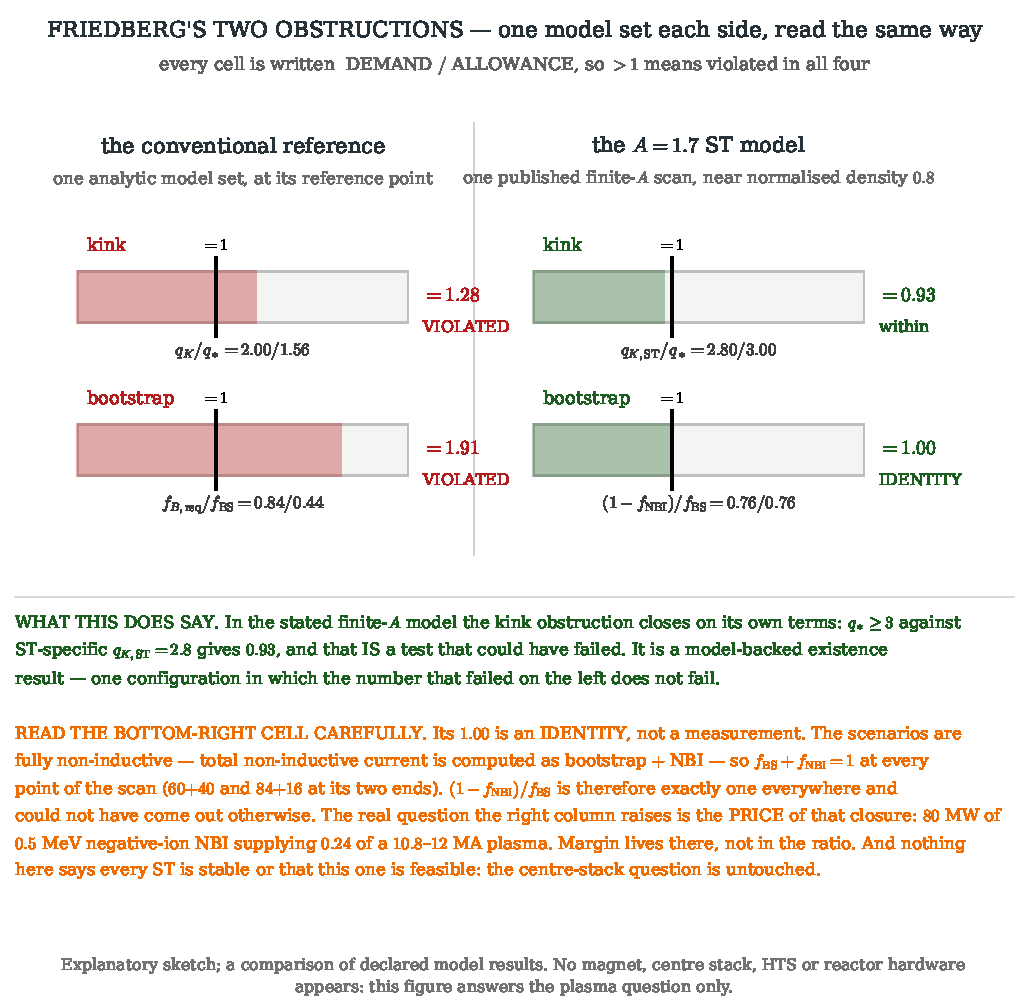
\includegraphics[width=1.0\textwidth]{figures/final/figS_st_closure.pdf}
\caption{Friedberg's two obstructions, read with their required logical inputs visible. The ST kink comparison is an actual threshold test. The ST $0.76/0.24$ current split is an identity of Menard's fully non-inductive scenario, not an independent bootstrap-ratio pass: it identifies the external current the scenario must provide. Both columns are declared model results, not properties of tokamaks or of STs.}
  \label{fig:figS_st_closure}
\end{figure}


% ============================= PAGE 109 ==============================
\newpage
\section*{109. First answer: the ST candidate closes the kink obstruction}

The relevant ST disruption evidence used by Menard \emph{et al.} is more demanding
than Friedberg's conventional reference threshold: NSTX disruption data show a marked
increase in disruptivity below $q_*\simeq2.8$. Their stated ST design requirement is
therefore
\[
 q_{K,\rm ST}=2.8.
\]
\footnote{Menard \emph{et al.}, cited on page 105, Sec.~2.1.3. The numerical boundary
comes from an NSTX data-based stability/disruption criterion and remains profile,
wall, and operating-regime dependent.}
The same candidate scan gives $q_*\ge3$. Substitute these published values:
\begin{equation}
 {\cal R}_{K,\rm ST}=\frac{2.8}{q_*}
\le\frac{2.8}{3.0}=0.93<1.
 \label{eq:st-kink-closure}
\end{equation}

This is an affirmative answer to Friedberg's kink obstruction within the declared
finite-$A$ model. It does not claim that every ST is kink stable; it demonstrates
that the low-$A$ candidate can satisfy a stricter ST-specific safety-factor criterion
than the $q_K=2$ criterion that the conventional reference failed. The geometrical
reason anticipated on page 104 is now joined to an explicit operating-point test.

% ============================= PAGE 110 ==============================
\newpage
\section*{110. The bootstrap result identifies the price; it does not yet test Friedberg's constraint}

The current ledger does not change with aspect ratio:
\[
 I_{\rm ST}=I_{\rm BS}+I_{\rm CD}.
\]
Divide by $I_{\rm ST}$. The Menard candidate gives, to the precision supported by
the published scan,
\[
 \frac{I_{\rm BS}}{I_{\rm ST}}\simeq0.76,\qquad
 \frac{I_{\rm CD}}{I_{\rm ST}}\simeq0.24,
\]
and the two fractions sum to one. This equality is not an independent test. The
Menard scenario is constructed to be fully non-inductive, so
\[
 \frac{I_{\rm BS}}I+\frac{I_{\rm CD}}I=1
\]
by its current-accounting definition. Dividing its own complement by its own
bootstrap fraction produces $1$ identically; it could not reveal a failure.

What the published point does give us is the physical and engineering burden that
an independent Friedberg test must meet:
\begin{equation}
 I_{\rm CD,needed}=(1-f_{\rm BS})I\simeq0.24I
 =2.6\text{--}2.9\,\mathrm{MA}.
 \label{eq:st-current-drive-needed}
\end{equation}
The scenario assumes $80\,\mathrm{MW}$ of $0.5\,\mathrm{MeV}$ neutral-beam
heating/current-drive power to obtain this fully non-inductive balance. It therefore
demonstrates a substantial finite-$A$ bootstrap fraction and states the associated
external-drive burden; it does not independently establish that a plant can afford
that burden.

The proper Friedberg test remains conditional until an economic/recirculating-power
analysis supplies $I_{\rm CD,allow}$ independently:
\begin{equation}
 {\cal R}_{B,\rm ST}=
\frac{1-I_{\rm CD,allow}/I}{f_{\rm BS}}\le1
\quad\Longleftrightarrow\quad
 I_{\rm CD,allow}\ge I_{\rm CD,needed}.
 \label{eq:st-bootstrap-conditional-closure}
\end{equation}
This is the question the next research pass must answer. It is more rigorous than
calling the identity $0.76/0.76=1$ a measured closure.

% ============================= PAGE 111 ==============================
\newpage
\section*{111. Verdict: ST closes the kink obstruction; bootstrap closure has a stated condition}

The published finite-aspect-ratio ST model answers one of Friedberg's two
current-centred obstructions affirmatively:
\[
 {\cal R}_{K,\rm ST}\le0.93<1.
\]
It also demonstrates a large bootstrap fraction, $f_{\rm BS}\simeq0.76$, and makes
the missing condition quantitative: the operating point needs approximately
$2.6$--$2.9\,\mathrm{MA}$ of independently affordable current drive.

We must not call that second result closure until its current-drive allowance has
been obtained independently. Friedberg's conventional comparison was meaningful
because the permitted drive came from a separate recirculating-power calculation
while the bootstrap fraction came from a neoclassical calculation. Reusing the
complement of a fully non-inductive ST current balance would erase that distinction.

\designconsequence{Low aspect ratio has now been shown to close the kink obstruction
in a published finite-$A$ model and to raise the bootstrap fraction to a quantified,
promising level. Whether it closes Friedberg's bootstrap obstruction depends on the
separate question $I_{\rm CD,allow}\ge2.6$--$2.9\,\mathrm{MA}$.}

% ============================= PAGE 112 ==============================
\newpage
\section*{112. Only after that answer does the separate centre-stack problem begin}

The conclusion on page 111 does not say that the ST has no further problems. It says
the kink question is answered affirmatively and the bootstrap question has been
reduced to an explicit independent current-drive requirement. Lowering $A$ simultaneously brings
the plasma closer to the symmetry axis and strengthens the inboard toroidal field.
That creates a new engineering question: can a D--T reactor fit shielding, breeding,
TF conductor, support, cooling, protection, and perhaps current-initiation function
inside the remaining central radius?

That question is logically separate. It cannot retroactively turn the resolved kink
ratio into a failure, any more than it can replace the independent current-drive
analysis still required for bootstrap closure. The remainder of this chapter changes
its subject explicitly: from \emph{what does low-$A$ plasma physics change?} to
\emph{what engineering debt does the low-$A$ solution create, and can HTS help pay
it?}

% ============================= PAGE 113 ==============================
\newpage
\section*{113. The same geometry takes radial space away from the centre stack}

The inboard radial ledger is the unavoidable counterargument. Let $c_{\rm cs}$ denote
the radial build occupied by the centre-stack TF conductor, its structural case,
insulation, cooling, and any allocated central-solenoid function. The innermost
radius available to the toroidal field is
\begin{equation}
 R_{\rm cs}=R_0-a-b-c_{\rm cs}
=R_0\left(1-\frac1A\right)-b-c_{\rm cs}.
 \label{eq:centre-stack-radius}
\end{equation}
The same $BR=\mathrm{constant}$ relation now gives
\begin{equation}
 B_{\rm cs}=\frac{B_0R_0}{R_{\rm cs}},\qquad
 B_0=B_{\rm cs}
\left[1-\frac1A-\frac{b+c_{\rm cs}}{R_0}\right].
 \label{eq:centre-stack-field}
\end{equation}
Every term in the square bracket has a physical meaning. Lowering $A$ subtracts
geometric room; $b$ is demanded by neutrons; $c_{\rm cs}$ is demanded by current,
structure, insulation, cooling, and possibly start-up flux. The bracket must be
positive even before a usable central field can exist.

As $A\rightarrow1$, the purely geometric factor $1-1/A$ tends to zero. No improved
plasma stability can reverse that subtraction. A low-$A$ reactor must instead choose
among a larger $R_0$, thinner-but-credible inboard nuclear and magnet systems, a
higher permissible $B_{\rm cs}$, different start-up/current-drive architecture, or
some combination. This is the centre-stack problem in its most elementary form.

\imagebrief{Cumulative construction state: low aspect ratio reveals the centre stack}
{Start with the complete conventional radial-build state, then reduce $A$ while
preserving the plasma, first wall/nuclear island $b$, and TF function. On the inboard
side show the shrinking interval $R_{\rm cs}=R_0-a-b-c_{\rm cs}$. Split
$c_{\rm cs}$ into conductor, structure, insulation/cooling, and optional central-
solenoid allocation. Label $B_0$ at the plasma and $B_{\rm cs}$ at the central
column. The image must show that low $A$ improves some plasma geometry while making
this physical interval scarce; do not depict a solved reactor.}

\begin{figure}[htbp]\centering
  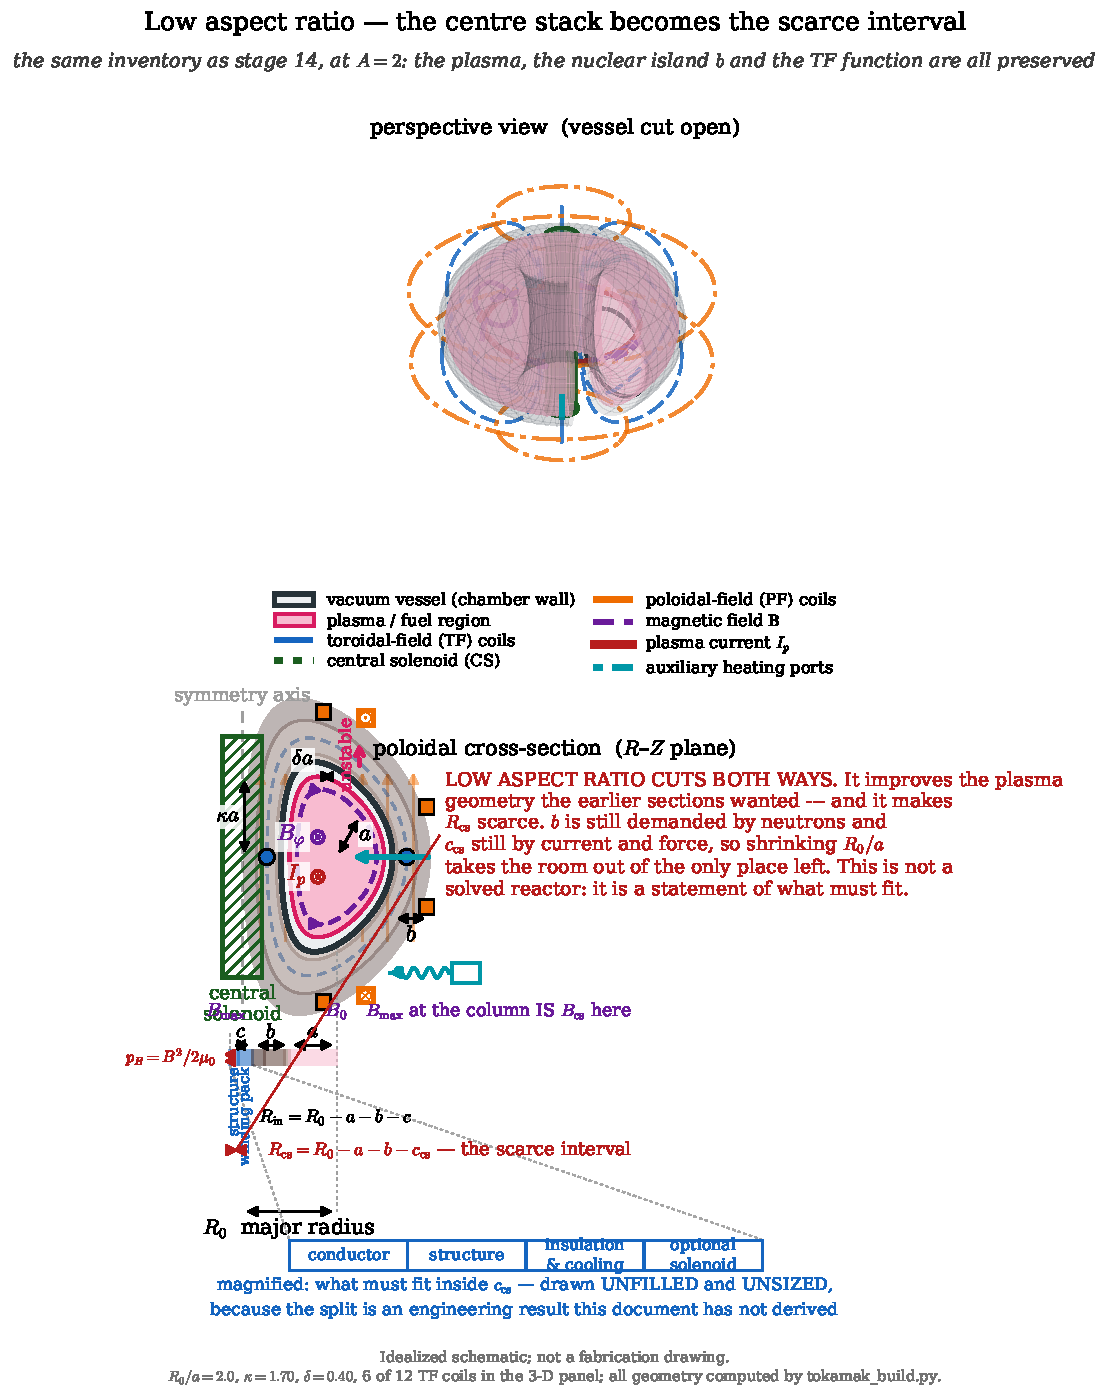
\includegraphics[width=1.0\textwidth]{figures/final/figM16_centrestack_tall.pdf}
  \caption{The same inventory as the complete radial build, at $A=2$: the plasma, the nuclear island $b$ and the TF function are all preserved --- only the aspect ratio changes. What changes with it is the room left for $R_{\rm cs}$. The magnified strip is drawn unfilled and unsized on purpose: that split is an engineering result this document has not derived.}
  \label{fig:figM16_centrestack_tall}
\end{figure}


% ============================= PAGE 114 ==============================
\newpage
\section*{114. HTS is a centre-stack lever, not a centre-stack eraser}

Equation~\eqref{eq:centre-stack-field} explains why HTS becomes especially valuable
in a low-aspect-ratio branch. For fixed desired $B_0$, reducing $A$ raises the
required central-column field $B_{\rm cs}$. A conductor with credible operating
current margin at higher field can make a smaller or more capable centre stack
possible. It may therefore preserve some of the low-$A$ gain that an ordinary
conductor field ceiling would otherwise erase.

But the same equation returns us to page 47:
\[
 p_B=\frac{B_{\rm cs}^2}{2\mu_0}.
\]
The central column must carry that magnetic loading while remaining manufacturable,
cooled, electrically insulated, protected, and maintainable in a neutron environment.
HTS does not turn $c_{\rm cs}$ into zero; its conductor and support still occupy
space, and higher field can increase the structural allocation. The central column
also competes with shielding and tritium-breeding volume, which cannot be dismissed
for a D--T plant.

\designconsequence{HTS can raise the credible field ceiling in the precise radial
interval that low aspect ratio makes scarce. It is a powerful enabling lever for an
ST, but it cannot by itself close the centre-stack equation.}

% ============================= PAGE 115 ==============================
\newpage
\section*{115. What remains after an ST closes Friedberg's two constraints}

The narrowly posed Friedberg result is now established on page 111. It does not
settle every physical or engineering demand placed on a reactor. The following
questions are separate and still require an integrated calculation:

\begin{enumerate}
\item a finite-aspect-ratio equilibrium and stability calculation, rather than the
large-aspect-ratio kink and Troyon closures;
\item a finite-aspect-ratio neoclassical bootstrap and current-drive calculation,
with explicit profiles and collisionality;
\item a transport and confinement basis applicable to the intended ST regime;
\item a radial centre-stack design that makes the bracket in
Eq.~\eqref{eq:centre-stack-field} positive with credible stress, current density,
shielding, cooling, protection, and maintenance margins;
\item a divertor, first-wall, blanket, and tritium-breeding calculation. This includes
the exhaust problem Friedberg's four ratios intentionally did not close.
\end{enumerate}

The centre-stack calculation begins next. Its task is not to reopen the two
Friedberg ratios; those have already been tested. Its task is to measure the exact
geometric and mechanical debt created by the low-$A$ solution. Only then can HTS,
reduced shielding, larger radius, alternative current initiation, or modular
maintenance be discussed as quantified responses rather than wishful labels.

% ============================= PAGE 116 ==============================
\newpage
\section*{116. The central column cannot evade Ampere's law}

The toroidal field outside an axis-enclosing current path obeys
\[
 B_\varphi(R)=\frac{\mu_0NI}{2\pi R}.
\]
Evaluate it at the plasma centre:
\begin{equation}
 NI=\frac{2\pi R_0B_0}{\mu_0}.
 \label{eq:centre-stack-ampere-turns}
\end{equation}
This is a striking centre-stack fact. The required TF ampere-turns are set by the
desired plasma product $R_0B_0$, not by the small radius of the central column. Moving
the current path inward raises the local field so that $RB_\varphi$ remains constant;
it does not make the required enclosed current disappear.

Let $J_{\rm wp,cs}$ be the allowed winding-pack current density after conductor,
stabilizer, insulation, cooling, joints where relevant, and allocated structural
fraction are counted honestly. The current-carrying cross-sectional area has the
necessary lower bound
\begin{equation}
 A_{\rm wp,cs}\ge
\frac{NI}{J_{\rm wp,cs}}
=\frac{2\pi R_0B_0}{\mu_0J_{\rm wp,cs}}.
 \label{eq:centre-stack-winding-area}
\end{equation}
It is a lower bound because a real column also needs support and non-conductor
functions. The equation makes the danger of vague compactness claims visible:
low aspect ratio shrinks the available column, while the TF current-carrying area
is controlled by the plasma field target.

% ============================= PAGE 117 ==============================
\newpage
\section*{117. A first necessary radius inequality for the centre stack}

Even in the unrealistically generous case that the entire circular column were
available to the TF winding pack,
\[
 \pi R_{\rm cs}^2\ge A_{\rm wp,cs}.
\]
Substitute Eq.~\eqref{eq:centre-stack-winding-area}:
\begin{equation}
 R_{\rm cs}\ge
\left(\frac{2R_0B_0}{\mu_0J_{\rm wp,cs}}\right)^{1/2}.
 \label{eq:centre-stack-radius-current-bound}
\end{equation}
This is not a design formula. It is a necessary condition with every real allocation
set to zero except current-carrying area. A credible design needs a stronger
inequality,
\begin{equation}
 \pi R_{\rm cs}^2\ge
 A_{\rm wp,cs}+A_{\rm str}+A_{\rm ins/cool}+A_{\rm sol}
+A_{\rm margin},
 \label{eq:centre-stack-area-ledger}
\end{equation}
where $A_{\rm str}$ carries magnetic load, $A_{\rm ins/cool}$ provides electrical and
thermal function, $A_{\rm sol}$ is any central-solenoid allocation, and the final
term represents manufacturing, protection, and operational margin.

Combine Eq.~\eqref{eq:centre-stack-radius} with
Eq.~\eqref{eq:centre-stack-area-ledger}. Lowering $A$ reduces the left-side geometric
radius, while the right side is set by field, materials, and operating functions.
The centre-stack problem is therefore a geometric inequality test. It can fail before
we ask whether the plasma is stable.

\designconsequence{A proposed ST must publish a centre-stack area ledger, not merely
an aspect ratio and a peak field. Without the conductor, structure, shielding, and
start-up allocations, there is no check that the proposed central column exists.}

% ============================= PAGE 118 ==============================
\newpage
\section*{118. Higher central field helps the plasma only by increasing mechanical demand}

At the centre-stack radius, the local magnetic-pressure scale is
\[
 p_{B,\rm cs}=\frac{B_{\rm cs}^2}{2\mu_0}.
\]
If a representative structural load path of area $A_{\rm load}$ is carried by
material limited to $\sigma_{\rm allow}$, force balance requires
\begin{equation}
 A_{\rm str}\gtrsim
\frac{p_{B,\rm cs}}{\sigma_{\rm allow}}A_{\rm load}.
 \label{eq:centre-stack-structure-bound}
\end{equation}
The detailed geometry determines $A_{\rm load}$ and the actual stress distribution;
the quadratic field dependence is already inescapable. As low $A$ reduces
$R_{\rm cs}$, Eq.~\eqref{eq:centre-stack-field} pushes $B_{\rm cs}$ upward for a
fixed $B_0$. The winding pack and its supporting structure then compete for the same
shrinking area.

HTS can improve the conductor part of the ledger by providing useful current margin
at higher field. It does not make the structural fraction vanish. In fact, if a
design uses the higher field that HTS enables, Eq.~\eqref{eq:centre-stack-structure-bound}
can require more support. That is why a high-field ST must report both conductor
performance and a credible mechanical case.

\model{Equation~\eqref{eq:centre-stack-structure-bound} is a lower-bound scaling,
not a finite-element stress certification. Real centre columns need three-dimensional
load paths, strain limits for the superconductor, cyclic-fatigue analysis, joints and
terminations where used, electrical insulation, quench or fault protection, and
neutron-degraded material properties.}

% ============================= PAGE 119 ==============================
\newpage
\section*{119. The transformer also loses flux swing as the column shrinks}

The transformer argument from page 20 gives a second, independent centre-stack
constraint. A solenoid of effective radius $R_{\rm sol}$ changes linked magnetic flux
by the scale
\begin{equation}
 \Delta\Psi_{\rm sol}\sim\pi R_{\rm sol}^2\Delta B_{\rm sol}.
 \label{eq:centre-stack-flux-swing}
\end{equation}
Faraday's law converts this flux swing into the volt-seconds available to initiate
and ramp plasma current. Since $R_{\rm sol}$ must fit inside the same central column,
$R_{\rm sol}<R_{\rm cs}$, the available inductive flux falls at least quadratically
as the column becomes narrow.

This fact connects directly to the Friedberg current ledger. A pulsed ST cannot
claim steady operation simply because it can make an initial plasma current; it needs
enough flux swing for its chosen pulse or a non-inductive start-up and sustainment
route. Conversely, a steady-state ST with high bootstrap fraction has a second
incentive to develop non-inductive current initiation: it can release central-column
area otherwise reserved for a large solenoid.

The choice is an engineering-plasma co-design decision. Removing solenoid allocation
from Eq.~\eqref{eq:centre-stack-area-ledger} may help the radial ledger, but transfers
an obligation to radio-frequency, neutral-beam, helicity-injection, or other
start-up/current-drive systems. It cannot be deleted from the thesis by a diagram.

% ============================= PAGE 120 ==============================
\newpage
\section*{120. The central-stack test is now ready to be made quantitative}

The equations above turn the phrase centre-stack problem into five checkable
questions:
\begin{enumerate}
\item What $B_0$, $R_0$, and $A$ are demanded by the plasma mission?
\item Does Eq.~\eqref{eq:centre-stack-field} leave positive inboard radius after
the required nuclear build $b$?
\item Does the available $\pi R_{\rm cs}^2$ exceed the full area ledger in
Eq.~\eqref{eq:centre-stack-area-ledger}?
\item Can the structural allocation carry the field-dependent load without exceeding
stress or superconducting-strain limits?
\item If solenoid area is reduced, what explicit non-inductive start-up and current
maintenance system replaces its flux swing?
\end{enumerate}

The next step is not to assign convenient answers. We will define a transparent
reference ST radial ledger and vary its field, radius, shielding, conductor current
density, and solenoid allocation. That will identify whether an HTS-enabled central
stack can close geometrically, where it fails, and which missing technologies would
have to carry the remaining burden.

% ============================= PAGE 121 ==============================
\newpage
\section*{121. A published ST study shows why the ledger must be literal}

It is useful to test the preceding geometry against a published allocation, provided
we do not mistake one study's choices for universal constants. Menard \emph{et al.}
examined an illustrative FNSF configuration with $A=2$, $R_0=1.87\,\mathrm m$, and
a $30\,\mathrm{cm}$ centre-column radius. Their stated inboard nuclear protection
included approximately $60\,\mathrm{cm}$ of water-cooled tungsten-carbide shielding;
the corresponding radial picture also includes a $2\,\mathrm{cm}$ first wall.
Their magnet assessment used a $70\,\mathrm{MA\,m^{-2}}$ winding-pack current-density
assumption and imposed both support-stress and superconducting-strain constraints.
\footnote{Menard \emph{et al.}, cited on page 105, Secs.~2.1 and 5.1,
especially their Figs.~46--47. The numbers in this paragraph are inputs and results
of that particular FNSF study, not universal requirements.}

The first calculation needs no plasma model. At $A=2$,
\[
 a=\frac{R_0}{A}=0.935\,\mathrm m,\qquad R_0-a=0.935\,\mathrm m.
\]
Temporarily subtract only the stated shield and first-wall thickness:
\begin{equation}
 0.935-0.600-0.020=0.315\,\mathrm m.
 \label{eq:menard-geometry-check}
\end{equation}
This rough geometry check is close to the study's $0.30\,\mathrm m$ centre-column
radius. It is not an argument that $15\,\mathrm{mm}$ is spare room: it says that
even before every cable, support, coolant channel, tolerance, and current-initiation
function is drawn, the low-$A$ inboard budget is already measured in centimetres.

\designconsequence{The centre stack is not an abstract penalty applied after plasma
optimization. A realistic neutron shield can consume most of the inboard radius in
an $A\simeq2$ machine. A claimed compact ST must display its own radial ledger with
the same honesty.}

% ============================= PAGE 122 ==============================
\newpage
\section*{122. Why a D--T centre stack begins with shielding, not conductor}

The inboard build $b$ in Eq.~\eqref{eq:centre-stack-radius} is not a decorative
engineering margin. D--T fusion emits $14.1\,\mathrm{MeV}$ neutrons, which are
uncharged. Magnetic confinement does not bend them. They stream into the first wall,
blanket, shield, structural material, and magnets; a reactor must absorb their heat,
breed tritium from lithium, and keep radiation damage to components within their
allowed lifetime.

That is why the $60\,\mathrm{cm}$ shield in the illustrative calculation on page 121
cannot simply be traded for a better magnet. It was a neutron-protection choice for
the study's mission and material assumptions. Changing it demands a new neutronics,
heating, lifetime, and tritium-breeding calculation. The same study found that at
low aspect ratio the inboard side can also be important to a tritium-breeding
solution.\footnote{Menard \emph{et al.}, cited on page 105, discuss the inboard
shielding and breeding allocation in their Sec.~5.3. Their conclusion is
configuration-specific; the general point here is only that breeding and shielding
claim radial space before the magnet is sized.}

This gives the radial order of operations:
\[
\boxed{\text{plasma mission}}
\ \longrightarrow\
\boxed{\text{neutron, heat, and tritium functions}}
\ \longrightarrow\
\boxed{\text{space left for TF conductor, support, and start-up}}.
\]
Reversing that order---choosing a desired tiny centre column first and assigning
the nuclear functions whatever space survives---would be the same category error
as assuming a finished tokamak at page 1. The nuclear build is a design demand that
helps reveal the permitted machine shape.

\imagebrief{Cumulative ST radial ledger: a neutron first, magnet second construction}
{Draw one clean outboard-midplane to inboard-midplane cross-section for the illustrative
$A=2$, $R_0=1.87\,\mathrm m$ state. On the inboard side add components in causal
order: plasma edge, first wall, approximately $0.60\,\mathrm m$ shielding as a
study-specific allocation, then the approximately $0.30\,\mathrm m$ central-column
envelope. Inside that envelope use unfilled subdivisions for TF winding, support,
insulation/cooling, and optional solenoid--do not assert their final sizes. Include
the arithmetic of Eq.~(\ref{eq:menard-geometry-check}) and a clear illustrative
published-allocation, not-universal-reactor-template note.}

\begin{figure}[htbp]\centering
  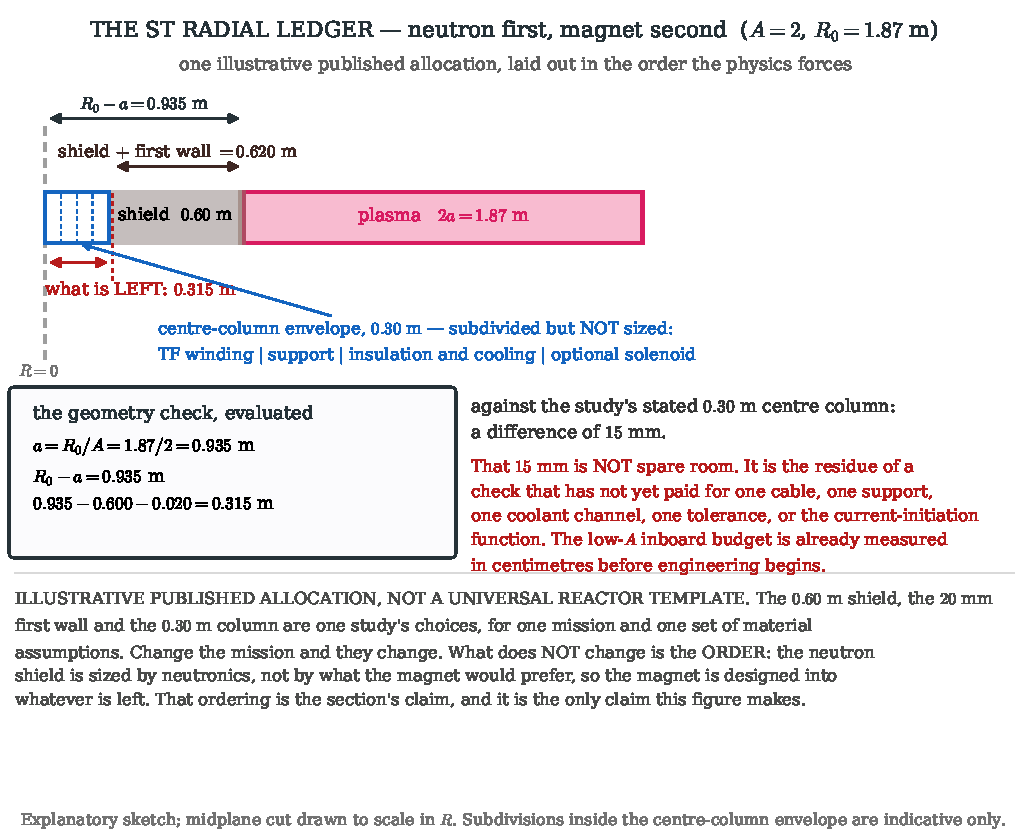
\includegraphics[width=1.0\textwidth]{figures/final/figS_st_radial_ledger.pdf}
  \caption{The published illustrative allocation, laid out in the order the physics forces: shield first, magnet into what is left. The arithmetic is Eq.~\eqref{eq:menard-geometry-check} evaluated. The $15$ mm difference from the study's stated column radius is not spare room --- it is the residue of a check that has not yet paid for one cable, support, coolant channel or tolerance.}
  \label{fig:figS_st_radial_ledger}
\end{figure}


% ============================= PAGE 123 ==============================
\newpage
\section*{123. What HTS changes in this ledger}

HTS changes a specific term: the credible current density and operating field margin
of the TF winding pack. In the necessary bound,
\[
 A_{\rm wp,cs}\ge
\frac{2\pi R_0B_0}{\mu_0J_{\rm wp,cs}},
\]
raising a credibly usable $J_{\rm wp,cs}$ reduces the \emph{minimum} current-carrying
area for a prescribed $R_0B_0$. It can therefore create room that a conventional
conductor cannot. In the field relation
\[
 B_{\rm cs}=\frac{B_0R_0}{R_{\rm cs}},
\]
HTS can also make a larger central field technically plausible without immediately
crossing the conductor's critical surface.

Those are real levers, but neither equation says that the whole right side of
Eq.~\eqref{eq:centre-stack-area-ledger} scales down as $1/J_{\rm wp,cs}$. The support,
insulation, cooling, protection, radiation, and manufacturing terms remain. Moreover,
raising $B_{\rm cs}$ raises $p_{B,\rm cs}\propto B_{\rm cs}^2$, which can enlarge the
structural term. A good HTS design may close the equation; HTS alone is not the
missing calculation.

The published low-$A$ work gives a concrete architectural direction rather than a
shortcut. A later $A=2$, $R_0=3\,\mathrm m$ HTS pilot-plant concept places all
superconducting poloidal-field coils outside the TF system, uses continuous HTS TF
coils, retains only a small central solenoid, and keeps inboard blanket/shield
functions in the radial build.\footnote{Menard \emph{et al.}, cited on page 105,
Sec.~5.4 and Fig.~53. It is a conditional systems study, not a demonstration that
every one of its performance targets has been experimentally achieved.} Each choice
answers one item in the ledger: outside PF coils avoid consuming central volume;
a small solenoid makes non-inductive start-up more important; HTS improves the TF
field option; blanket and shield remain non-negotiable.

\designconsequence{HTS is the enabling material in a co-design, not an exemption
from the co-design. Its success must be reported as a closed area, stress, radiation,
and start-up ledger at the chosen $R_0$, $A$, and $B_0$.}

% ============================= PAGE 124 ==============================
\newpage
\section*{124. What remains after the Friedberg answer}

The causal argument has reached a useful, deliberately narrow conclusion. The
finite-$A$ calculation on pages 106--111 answered Friedberg's two current questions.
The earlier first-principles geometry explains why that answer was possible:
\begin{enumerate}
\item Eq.~\eqref{eq:aspect-ratio-q-beta} changes the current--safety-factor geometry
in the favorable direction for the kink/current coupling.
\item Eq.~\eqref{eq:aspect-ratio-trapped-fraction} strengthens the trapping physics
that underlies a route to bootstrap current.
\end{enumerate}
HTS then supplies a plausible material lever for the adverse inboard field and
winding-area problem created by the same geometry. Published integrated ST studies
show that these ingredients can be put into a serious systems calculation.

That establishes the result relevant here: a specified finite-$A$ ST model closes the
two current-centred constraints that failed in Friedberg's conventional baseline,
whereas merely raising $H$ in that baseline did not. It does not establish a theorem
that every ST or every other reactor constraint is closed; exhaust, blanket, tritium,
radiation, maintenance, and cost remain their own questions.

The next calculation must therefore have two ledgers, evaluated together:
\[
\begin{array}{c|c}
\text{finite-$A$ plasma ledger} & \text{centre-stack reactor ledger}\\ \hline
q,\ \beta_N,\ \text{equilibrium/stability} &
b,\ R_{\rm cs},\ A_{\rm wp},\ A_{\rm str}\\
\text{bootstrap and driven current} &
\text{shield, breeding, stress, start-up}\\
\text{transport and exhaust} &
\text{HTS margin, protection, maintenance}
\end{array}
\]
The next section makes the centre-stack ledger into an explicit, auditable parameter
scan. It does not relabel that separate engineering question as a failed Friedberg
plasma constraint.

% ============================= PAGE 125 ==============================
\newpage
\section*{125. A dimensionless necessary test for a central TF winding}

For a first scan, reserve the inboard nuclear build $b$ before allocating the central
column. The outer radius of the column envelope is then
\begin{equation}
 R_{\rm env}=R_0\left(1-\frac1A\right)-b.
 \label{eq:centre-stack-envelope}
\end{equation}
This is deliberately more generous than a finished design: it gives every remaining
square millimetre to the central column before deciding how much is conductor,
structure, cooling, or solenoid.

Let $f_{\rm wp}$ be the fraction of the envelope's circular cross-sectional area that
the designer has explicitly allocated to the TF winding pack. It is an accounting
input, not a material constant. Equation~\eqref{eq:centre-stack-winding-area} then
requires
\[
 \frac{2\pi R_0B_0}{\mu_0J_{\rm wp,cs}}
\le f_{\rm wp}\pi R_{\rm env}^2.
\]
After cancelling $\pi$, define the dimensionless winding occupancy
\begin{equation}
 \eta_{\rm wp}\equiv
 \frac{2R_0B_0}
 {\mu_0J_{\rm wp,cs}\left[R_0(1-1/A)-b\right]^2}.
 \label{eq:centre-stack-winding-occupancy}
\end{equation}
The necessary test is simply
\begin{equation}
 \eta_{\rm wp}\le f_{\rm wp}<1.
 \label{eq:centre-stack-winding-test}
\end{equation}
If $\eta_{\rm wp}>1$, even a column made entirely of winding pack cannot carry the
required TF current. If $f_{\rm wp}<\eta_{\rm wp}<1$, a central column exists only
on paper because the current pack has consumed space explicitly promised to the
other functions.

\model{This is a necessary electromagnetic-area test. It treats the winding pack as
uniformly current carrying and does not certify field quality, stress, strain,
quench protection, neutron lifetime, joints, penetrations, or manufacturability.
Those omissions make passing the test easier, never harder.}

% ============================= PAGE 126 ==============================
\newpage
\section*{126. Solving the test exposes a lower-aspect-ratio boundary}

The test can be solved for the smallest aspect ratio permitted by the chosen
area allocation. Take the positive square root of
Eq.~\eqref{eq:centre-stack-winding-test}:
\[
 R_0\left(1-\frac1A\right)-b
\ge
\left(\frac{2R_0B_0}{\mu_0J_{\rm wp,cs}f_{\rm wp}}\right)^{1/2}.
\]
Divide by $R_0$ and rearrange:
\begin{equation}
 A\ge A_{\min,\rm wp}\equiv
\left[
1-\frac{b}{R_0}
-\left(\frac{2B_0}
{\mu_0J_{\rm wp,cs}f_{\rm wp}R_0}\right)^{1/2}
\right]^{-1}.
\label{eq:centre-stack-aspect-bound}
\end{equation}
The bracket must be positive. If it is zero or negative, the stated $R_0$, $B_0$,
nuclear build, winding-pack current density, and allocation cannot coexist at
\emph{any} aspect ratio in this simplified central-column arrangement.

Every trend in this equation has a physical reading:
\begin{itemize}
\item Increasing $B_0$ increases the required ampere-turns and raises the minimum
allowed $A$.
\item Increasing $b/R_0$ claims the inboard radius for nuclear function and raises
the minimum allowed $A$.
\item Increasing credible $J_{\rm wp,cs}$ or giving the winding pack a larger
honest fraction $f_{\rm wp}$ lowers the electromagnetic area demand.
\item Increasing $R_0$ helps twice: the nuclear build occupies a smaller fraction
of the radius and the required winding area is less crowded into the column.
\end{itemize}
The last two points identify exactly what HTS and a less compact plant can improve.
They also show why neither word automatically guarantees a viable ST.

% ============================= PAGE 127 ==============================
\newpage
\section*{127. A transparent teaching scan: field makes the low-$A$ limit move}

Use the deliberately declared teaching inputs
\[
 R_0=3.0\,\mathrm m,\quad b=0.65\,\mathrm m,\quad
 J_{\rm wp,cs}=70\,\mathrm{MA\,m^{-2}},\quad f_{\rm wp}=0.40.
\]
The current-density scale is comparable to an assumption used in the illustrative
Menard study on page 121; the radius, nuclear build, and $40\%$ allocation here are
\emph{not} a proposed reactor. They merely make the algebra visible. Substitution in
Eq.~\eqref{eq:centre-stack-aspect-bound} gives:
\[
\begin{array}{c|c|c}
B_0\;(\mathrm T) & A_{\min,\rm wp} & \eta_{\rm wp}\ \text{at }A=2\\ \hline
4 & 1.97 & 0.378\\
6 & 2.24 & 0.567\\
8 & 2.54 & 0.756
\end{array}
\]
At $A=2$, the available envelope radius is
$R_{\rm env}=3(1-1/2)-0.65=0.85\,\mathrm m$. The first row barely clears the
assigned $40\%$ winding allocation. The latter two do not: they require more winding
area than has been allocated even before support, insulation, cooling, or a solenoid
are tested. The table is reproducible from
\texttt{centre\_stack\_ledger.py}; every input is displayed at the top of that file.

This is the exact sense in which HTS is a boost mechanism. If it raises the
\emph{credible system-level} $J_{\rm wp,cs}$ at the relevant field, temperature,
strain, radiation, and protection margin, it can lower $A_{\min,\rm wp}$. If the
design instead spends the HTS benefit to raise $B_0$, the square-root field penalty
pushes $A_{\min,\rm wp}$ upward. The net result is a co-design decision, not a
one-directional law.

\auditnote{Passing the $4\,\mathrm T$ row does not make it a reactor. The table omits
the structure term that grows with central field, the non-winding allocations, the
neutron and tritium calculation behind $b$, and all plasma/stability/exhaust tests.
It is intentionally a failure detector, not a feasibility certificate.}

\end{document}
